\documentclass[a4paper, 11pt]{article}

\usepackage[utf8]{inputenc}

\usepackage{
amssymb, amsmath, amsthm, amstext, amsfonts, amsopn, amscd, amsbsy,comment
}
\usepackage{mathrsfs, dsfont, mathdots}
\usepackage{bm}
\usepackage{accents}

\usepackage{graphicx}
\usepackage[usenames,dvipsnames]{xcolor}

\usepackage[colorlinks=true, linkcolor=black, breaklinks=true, citecolor=blue, urlcolor=red]{hyperref} 
\usepackage{float}
\usepackage{subcaption}
\usepackage{caption}
\usepackage{tikz}

\usepackage[numbers]{natbib}
%\bibliographystyle{natdin}
\bibliographystyle{abbrvnat}
\usepackage{url}
\setlength{\unitlength}{1mm}
\def\bottomfraction{.9}

\newlength{\dinwidth}
\newlength{\dinmargin}


%\usepackage[style=numeric, sorting=nyt, firstinits=true, backend=bibtex, url=false, isbn=false, doi=false, maxnames=10]{biblatex}
%{\small\bibliography{../../../../lib/library}}
%\renewcommand*{\bibfont}{\footnotesize}

\def\qed{{\unskip\nobreak\hfil\penalty50
\hskip2em\hbox{}\nobreak\hfil$\square$
\parfillskip=0pt \finalhyphendemerits=0\par}\medskip}
\def\proof{\trivlist \item[\hskip \labelsep{\bf Proof.\ }]}
\def\endproof{\null\hfill\qed\endtrivlist\noindent}

\renewcommand{\emptyset}{\varnothing}

% ++++ short cuts ++++

% +++++ colors +++++
\newcommand{\pc}{\color{purple}}
\newcommand{\bc}{\color{blue}}
\newcommand{\rc}{\color{red}}
\newcommand{\textb}{\textcolor{blue}}
\newcommand{\textr}{\textcolor{red}}
\newcommand{\texto}{\textcolor{orange}}
\newcommand{\textg}{\textcolor{green}}

% +++++ cal, frak, bold, etc. +++++

\newcommand{\fA}{\mathfrak{A}}\newcommand{\cA}{\mathcal{A}}\newcommand{\dA}{\mathds{A}}\newcommand{\sA}{\mathscr{A}}
\newcommand{\ua}{\textup a}
\newcommand{\fB}{\mathfrak{B}}\newcommand{\cB}{\mathcal{B}}\newcommand{\dB}{\mathds{B}}\newcommand{\sB}{\mathscr{B}}
\newcommand{\fC}{\mathfrak{C}}\newcommand{\cC}{\mathcal{C}}\newcommand{\dC}{\mathds{C}}\newcommand{\sC}{\mathscr{C}}
\newcommand{\fd}{\mathfrak{d}}\newcommand{\ud}{\textup{d}}
\newcommand{\fD}{\mathfrak{D}}\newcommand{\cD}{\mathcal{D}}\newcommand{\dD}{\mathds{D}}\newcommand{\sD}{\mathscr{D}}
\newcommand{\fE}{\mathfrak{E}}\newcommand{\cE}{\mathcal{E}}\newcommand{\dE}{\mathds{E}}\newcommand{\sE}{\mathscr{E}}
\newcommand{\fF}{\mathfrak{F}}\newcommand{\cF}{\mathcal{F}}\newcommand{\dF}{\mathds{F}}\newcommand{\sF}{\mathscr{F}}
\newcommand{\fg}{\mathfrak{g}}
\newcommand{\fh}{\mathfrak{h}}
\newcommand{\fH}{\mathfrak{H}}\newcommand{\cH}{\mathcal{H}}\newcommand{\dH}{\mathds{H}}\newcommand{\sH}{\mathscr{H}}
\newcommand{\fI}{\mathfrak{I}}\newcommand{\cI}{\mathcal{I}}
\newcommand{\fK}{\mathfrak{K}}\newcommand{\cK}{\mathcal{K}}
\newcommand{\fL}{\mathfrak{L}}\newcommand{\cL}{\mathcal{L}}
\newcommand{\fl}{\mathfrak{l}}\newcommand{\cl}{\mathcal{l}}
\newcommand{\fN}{\mathfrak{N}}\newcommand{\cN}{\mathcal{N}}\newcommand{\dN}{\mathds{N}}\newcommand{\sN}{\mathscr{N}}
\newcommand{\fO}{\mathfrak{O}}\newcommand{\cO}{\mathcal{O}}\newcommand{\dO}{\mathds{O}}\newcommand{\sO}{\mathscr{O}}
\newcommand{\fQ}{\mathfrak{Q}}
\newcommand{\fP}{\mathfrak{P}}\newcommand{\cP}{\mathcal{P}}\newcommand{\dP}{\mathds{P}}\newcommand{\sP}{\mathscr{P}}
\newcommand{\fR}{\mathfrak{R}}\newcommand{\cR}{\mathcal{R}}\newcommand{\dR}{\mathds{R}}\newcommand{\sR}{\mathscr{R}}
\newcommand{\fS}{\mathfrak{S}}\newcommand{\cS}{\mathcal{S}}\newcommand{\dS}{\mathds{S}}\newcommand{\sS}{\mathscr{S}}
\newcommand{\fT}{\mathfrak{T}}\newcommand{\cT}{\mathcal{T}}\newcommand{\dT}{\mathds{T}}\newcommand{\sT}{\mathscr{T}}
\newcommand{\fU}{\mathfrak{U}}\newcommand{\cU}{\mathcal{U}}\newcommand{\dU}{\mathds{U}}\newcommand{\sU}{\mathscr{U}}
\newcommand{\fu}{\mathfrak{u}}
\newcommand{\fW}{\mathfrak{W}}\newcommand{\cW}{\mathcal{W}}\newcommand{\dW}{\mathds{W}}\newcommand{\sW}{\mathscr{W}}
\newcommand{\fZ}{\mathfrak{Z}}\newcommand{\cZ}{\mathcal{Z}}\newcommand{\dZ}{\mathds{Z}}\newcommand{\sZ}{\mathscr{Z}}
\newcommand{\CC}{\mathbb{C}}\newcommand{\C}{\mathbb{C}}
\newcommand{\ZZ}{\mathbb{Z}}\newcommand{\Z}{\mathbb{Z}}
\newcommand{\TT}{\mathbb{T}}\newcommand{\T}{\mathbb{T}}\newcommand{\ft}{\mathfrak{t}}
\newcommand{\RR}{\mathbb{R}}\newcommand{\R}{\mathbb{R}}
\newcommand{\NN}{\mathbb{N}}\newcommand{\N}{\mathbb{N}}
\newcommand{\FF}{\mathbb{F}}



% +++++ greek letters +++++

\newcommand{\al}{\alpha}
\newcommand{\be}{\beta}
\newcommand{\ga}{\gamma}\newcommand{\Ga}{\Gamma}
\newcommand{\de}{\delta}\newcommand{\De}{\Delta}
\newcommand{\ep}{\epsilon}\newcommand{\vep}{\varepsilon}
\newcommand{\ka}{\kappa}
\newcommand{\la}{\lambda}\newcommand{\La}{\Lambda}
\newcommand{\rh}{\rho}
\newcommand{\si}{\sigma}
\renewcommand{\th}{\theta}
\newcommand{\om}{\omega} \newcommand{\Om}{\Omega}

% +++++ other stuff +++++

\newcommand{\non}{\nonumber}
\newcommand{\isom}{\cong}
\newcommand{\equi}{\sim}
\newcommand{\ti}{\tilde}
\newcommand{\ch}{\check}
\newcommand{\h}{\hat}
\newcommand{\lan}{\langle}
\newcommand{\ran}{\rangle}
\newcommand{\wh}{\widehat}
\newcommand{\wt}{\widetilde}

\newcommand{\Fock}{\mathcal{F}}
\newcommand{\tFock}{\widetilde{\Fock}}

\newcommand{\ltwo}{\ell^{2}}
\newcommand{\li}{\ell^{\infty}}

\newcommand{\ds}{\displaystyle}


% ++++ math operators ++++

\DeclareMathOperator{\Ad}{Ad}
\DeclareMathOperator{\ad}{ad}
\DeclareMathOperator{\id}{id}
\DeclareMathOperator{\1}{\mathds{1}}
\DeclareMathOperator{\tr}{tr}\DeclareMathOperator{\Tr}{Tr}
\DeclareMathOperator{\Str}{Tr_{s}}
\DeclareMathOperator{\pf}{pf}
\DeclareMathOperator{\vol}{vol}
\DeclareMathOperator{\Vect}{Vect}
\DeclareMathOperator{\Diff}{Diff}
\DeclareMathOperator{\Mob}{Mob}
\DeclareMathOperator{\Ker}{ker}
\DeclareMathOperator{\im}{im}
\DeclareMathOperator{\Ran}{ran}
\DeclareMathOperator{\Stab}{Stab}
\DeclareMathOperator{\Span}{Span}
\DeclareMathOperator{\wlim}{w-lim}
\DeclareMathOperator{\wslim}{w*-lim}
\DeclareMathOperator*{\slim}{s-lim}
\DeclareMathOperator{\Dim}{dim}
\DeclareMathOperator{\Ind}{Ind}
\DeclareMathOperator{\Aut}{Aut}
\DeclareMathOperator{\End}{End}
\DeclareMathOperator{\Hom}{Hom}
\DeclareMathOperator{\fn}{null}
\DeclareMathOperator{\ess}{ess}
\DeclareMathOperator{\supp}{supp}
\DeclareMathOperator{\ac}{\underset{t\to i}{\textnormal {anal.cont.\,}}}
\DeclareMathOperator{\CAR}{\textup{CAR}}
\DeclareMathOperator{\SDC}{\textup{SDC}}
\DeclareMathOperator{\TL}{\textup{TL}}
\DeclareMathOperator{\TIM}{\textup{TIM}}
\DeclareMathOperator{\sign}{\textup{sign}}
\DeclareMathOperator{\sinc}{sinc}
\DeclareMathOperator{\con}{\textup{cont.}}
\DeclareMathOperator{\sd}{sd}
\DeclareMathOperator{\std}{std}
\DeclareMathOperator{\per}{per}
\DeclareMathOperator{\alg}{alg}
\DeclareMathOperator{\Trig}{\textup{Trig}}
\DeclareMathOperator{\act}{\curvearrowright}

% ++++ other definitions ++++ remove unnecessary stuff

\def\aci{\underset{t\to -i}{\textnormal anal.cont.\,}}
\def\acb{\underset{t\to i\beta}{\textnormal {anal.cont.\,}}}
%\def\undertilde#1{\mathord{\vtop{\ialign{##\crcr
%$\hfil\displaystyle{#1}\hfil$\crcr\noalign{\kern1.5pt\nointerlineskip}
%$\hfil\tilde{}\hfil$\crcr\noalign{\kern1.5pt}}}}}

\def\Undertilde#1{\mathord{\vtop{\ialign{##\crcr
$\hfil\displaystyle{#1}\hfil$\crcr\noalign{\kern1.5pt\nointerlineskip}
$\hfil\widetilde{}\hfil$\crcr\noalign{\kern1.5pt}}}}}

\def\res{{\upharpoonright}}
\def\tPoi{\tilde{\cal P}_+^\uparrow}
\def\PSL{{{\rm PSL}(2,\RR)}}
\def\tPSL{{{\rm PSL}(2,\RR)}^{\tilde{}}}
\def\PSL{PSV(1,1)}
\def\Vir{{\rm Vir}}
\def\Svir{{\rm Svir}}
\def\Mob{{\rm\textsf{M\"ob}}}
\def\Mobn{{\rm\textsf{M\"ob}}^{(n)}}
\def\Mobb{{\rm\textsf{M\"ob}}^{(2)}}
\def\Mobi{{\rm\textsf{M\"ob}}^{(\infty)}}
\def\Si{\mathbb S_{\infty}}
\def\Sn{S^{1(n)}}
\def\S2{S^{1(2)}}
\def\Hi{\dH^{\infty}(\dS_{1/2})}
\def\Hp{\dH^{\infty}(\dS_{\pi})}
\def\Ha{\dH^{\infty}(\dS_{a})}
\def\vect{{{\rm Vect}(S^1)}}
\def\sl2{{{\rm SL}(2,\RR)}}
\def\psl2{{{\rm PSL}(2,\RR)}}
\def\u1{{{\rm V}(1)}}
\def\su2{{{\rm SV}(2)}}
\def\suN{{{\rm SV}(N)}}
\def\so3{{{\rm SO}(3)}}
\def\gk {{G_k}}
\def\SO{{\mathrm{SO}}}
\def\SLC{{\mathrm{SL}(2,\CC)}}

%++++ geometry and margins ++++

\setlength{\dinwidth}{21.0cm}
\setlength{\textwidth}{15.3cm}  %14.7
\setlength{\textheight}{23.4cm} %23.0

\setlength{\dinmargin}{\dinwidth}
\addtolength{\dinmargin}{-\textwidth}
\setlength{\dinmargin}{0.5\dinmargin}
\setlength{\oddsidemargin}{-1.0in}
\addtolength{\oddsidemargin}{\dinmargin}
\setlength{\evensidemargin}{\oddsidemargin}
\setlength{\marginparwidth}{0.9\dinmargin}
\setlength{\marginparsep}{8pt}
\setlength{\marginparpush}{5pt}

\setlength{\columnseprule}{0mm}
\setlength{\columnsep}{7mm}

\setlength{\topmargin}{-0.5in}
\setlength{\headheight}{30pt}
\setlength{\headsep}{10pt} 

\setlength{\footskip}{20pt}

%++++ theorem environments ++++

\def\proof{\noindent{\bf Proof. }}
\def\qed{$\Box$\medskip}
%THEOREMLIKE ENVIRONNEMENTS
\newtheorem{letterthm}{Theorem}
\renewcommand{\theletterthm}{\Alph{letterthm}}
\newtheorem{thmchap}{Theorem}
\newtheorem{thm}{Theorem} [section]
\newtheorem{prop}[thm]{Proposition}
%\newtheorem{proposition}[thm]{Proposition}
\newtheorem{lemma}[thm]{Lemma}
%\newtheorem{lemma}[thm]{Lemma}
\newtheorem{defn}[thm]{Definition}
\newtheorem{cor}[thm]{Corollary}
\newtheorem{rem}[thm]{Remark}
\newtheorem{example}[thm]{Example}
\newtheorem{criterion}[thm]{Criterion}
\newtheorem{conjecture}{Conjecture}
\newtheorem{assumption}{Assumption}
\newtheorem{hyp}[thm]{Hypothesis}
\newcommand{\Nop}{\mathsf{N}}
%\newtheorem{conjecture}{Conjecture}
%\newtheorem{criterion}[theoreme]{Criterion}

\newcommand{\sa}{\nin\bf Supporting arguments: \rm}
\newcommand{\bea}{\begin{assumption}}
	\newcommand{\eea}{\end{assumption}}
\newcommand{\beco}{\begin{conjecture} }
	\newcommand{\eeco}{\end{conjecture} }
\newcommand{\beq}{\begin{equation}}
	\newcommand{\eeq}{\end{equation}}
\newcommand{\beqa}{\begin{eqnarray}}
	\newcommand{\eeqa}{\end{eqnarray}}
\newcommand{\ben}{\begin{arabicenumerate}}
	\newcommand{\een}{\end{arabicenumerate}}
\newcommand{\bex}{\begin{example}}
	\newcommand{\eex}{\end{example}}
\newcommand{\ber}{\begin{remark}}
	\newcommand{\eer}{\end{remark}}
\newcommand{\bec}{\begin{corollary}}
	\newcommand{\eec}{\end{corollary}}
\newcommand{\bep}{\begin{proposition}}
	\newcommand{\eep}{\end{proposition}}
\newcommand{\becr}{\begin{criterion}}
	\newcommand{\eecr}{\end{criterion}}



\begin{document}

\tikzset{->-/.style={decoration={
  markings,
  mark=at position #1 with {\arrow{latex}}},postaction={decorate}}}

\title{Conformal field theory from lattice fermions}
\author{Tobias J. Osborne${}^{1}$, Alexander Stottmeister${}^{1}$}
\date{
\small{${}^{1}$ Institut f\"ur Theoretische Physik, Leibniz Universit\"at Hannover
\\Appelstra\ss e 2, 30167 Hannover, Germany} \\[0.5cm]
\today}
\maketitle
\begin{abstract}
We provide a rigorous lattice approximation of conformal field theories given in terms of lattice fermions in 1+1-dimensions, focussing on free fermion models and Wess-Zumino-Witten models. To this end, we utilize a recently introduced operator-algebraic framework for Wilson-Kadanoff renormalization. In this setting, we prove the convergence of the approximation of the Virasoro generators by the Koo-Saleur formula. From this, we deduce the convergence of lattice approximations of conformal correlation functions to their continuum limit. In addition, we show how these results lead to explicit error estimates pertaining to the quantum simulation of conformal field theories.
\end{abstract}

\tableofcontents

\section{Introduction}
\label{sec:intro}

A rigorous mathematical formulation of quantum field theory (QFT) is one the central challenges for the new millennium \cite{seibergNathanSeiberg20152014}. A variety of approaches to build a rigorous theory of QFT have been employed throughout the past decades and have lead to deep results and insights -- from \emph{constructive QFT} \cite{GlimmQuantumFieldTheory, glimmQuantumPhysicsFunctional1987, SummersAPerspectiveOn} to algebraic QFT \cite{HaagAnAlgebraicApproach, LechnerConstructionOfQuantum, BahnsLocalNetOf}, vertex operator algebras (VOAs) \cite{BorcherdsVertexAlgebrasKac, FrenkelVertexOperatorAlgebras, FrenkelBasicRepresentationsOf, TenerGeometricRealizationOf}, and beyond \cite{segalDefinitionConformalField2004, GrosseSolutionOfThe, GubinelliAPDEConstruction}. However, a completely satisfactory mathematical theory of QFT is still yet to be obtained. For this reason a proof of the rigorous existence of (and mass gap for) Yang-Mills theory was selected as one of the Clay maths prize problems. 

Several key difficulties to obtaining a rigorous formulation of QFT are already epitomized by $1+1$-dimensional gapless quantum field theories, in particular, \emph{conformal field theories} (CFTs) where a variety of constructions and classifications results has been obtained \cite{BelavinInfiniteConformalSymmetry, DiFrancescoCFTBook, EvansQuantumSymmetriesOn, WassermannOperatorAlgebrasAnd, BrunettiModularStructureAnd, GabbianiOperatorAlgebrasAnd, BuchholzTheCurrentAlgebra, KawahigashiClassificationOfLocal, CarpiFromVertexOperator}. 

A natural strategy to prove the existence of such a theory is to somehow realize it as the limit of a sequence of \emph{discretized approximations} (see \cite{JonesSomeUnitaryRepresentations, JonesANoGo, JonesScaleInvariantTransfer, BrothierConstructionsOfConformal, KlieschContinuumLimitsOf, OsborneQuantumFieldsFor} for recent attempts in a Hamiltonian setting), or \emph{lattice models}, on finite spatial lattices $\Lambda_{N} = \varepsilon_{N}\{-L_{N}, -L_{N} +1, \ldots, L_{N}-2, L_{N}-1\}\subset\varepsilon_{N}  \mathbb{Z}$, where $L=\varepsilon_N r_N$ is the length of the system. Associated to each lattice site $x\in \Lambda_N$ is a quantum degree of freedom, typically modeled by a Hilbert space $\mathcal{H}_x$, so that one assigns the \emph{total Hilbert space} $\mathcal{H}_{N} \subset \bigotimes_{x\in \Lambda_{N}} \mathcal{H}_x$ to the system\footnote{In the cases considered in this paper the total Hilbert space is provided by fermionic Fock space $\fF_{\ua}(\mathfrak{h}_{N})$ based on a one-particle space $\mathfrak{h}_{N}$ for a particle with spin hopping on $\Lambda_N$, which can be realised as subspace of a direct sum of tensor products of smaller Hilbert spaces.}. One requires, further, a \emph{Hamiltonian} $H_{0}^{(N)}$ for each discretization
\begin{align*}
H^{(N)}_0 = \tfrac{L}{\pi}\varepsilon_N\sum_{x\in\Lambda_N} h_x^{(N)},
\end{align*}
which is a sum of self-adjoint operators $h_x^{(N)}$ on $\mathcal{H}_N$ with finite support centered on $x$. A key additional ingredient that must be specified is a $C^{*}$-algebra $\mathfrak{A}_N$ (considered as a subalgebra of the bounded operators $B(\mathcal{H}_N)$ on $\cH_{N}$) of basic \emph{observables or fields}, corresponding to discretizations of their potential continuum counterparts. Given this data the task is to assign mathematical meaning to the \emph{scaling limit} of $\{\mathfrak{A}_N, \mathcal{H}_N, H^{(N)}_0\}$. 

A multitude of challenges must be overcome to realize this limit, in particular: (a) specifying the mathematical data to compare the discretizations with differing lattice size (and hence the topology for the limit); (b) identifying the correct lattice Hamiltonians for a target QFT; (c) proving the convergence of the sequence; and (d) proving that the requisite symmetry groups of the QFT are realized via projective unitary representations on the limit space. The recovery of expected continuum symmetries, i.e., requirement (d), typically poses severe difficulties (see \cite{SmirnovTowardsConformalInvariance, ChelkakUniversalityInThe, HonglerConformalFieldTheory, DuminilCopinRotationalInvarianceIn} for major advances in two-dimensional critical lattice models in the Euclidean framework).

The recently introduced \emph{operator-algebraic renormalization} (OAR) \cite{StottmeisterOperatorAlgebraicRenormalization, MorinelliScalingLimitsOf, BrothierConstructionsOfConformal} supplies a novel approach to defining, and proving the existence of, the above limit in Hamiltonian approach, thus overcoming the four challenges outlined in the previous paragraph. To do this one introduces the following additional structures:
\begin{itemize}
	\item \emph{Refining quantum channels}, which are unital completely positive (ucp) maps, $\alpha^{N}_{N+1}:\fA_{N}\rightarrow\fA_{N+1}$, connecting the observable algebras between the different scales. These induce dual \emph{coarse-graining} trace-preserving completely positive (tpcp) maps $\cE^{N+1}_{N}$ between the state spaces, or density matrices respectively preduals, $B(\cH_{N+1})_{*}\rightarrow B(\cH_{N})_{*}$, in the ultraweakly continuous case. Here, $B(\cH_{N})_{*}$ denotes the predual on $B(\cH_{N})$, i.e.~the trace-class operators on $\cH_{N}$.
	\item a sequence of initial (bare) states $\omega^{(N)}_{0}$ on the algebras $\mathfrak{A}_N$, possibly given by a density matrix $\rho^{(N)}_{0}\in B(\cH_{N})_{*}$, which are renormalized according to $\omega^{(N)}_{M} = \omega^{(N+M)}_{0}\circ\alpha^{N}_{N+M}$.
\end{itemize}
The scaling limit is then obtained via the Gelf'and-Naimark-Segal (GNS) construction\footnote{Informally, this means that the continuum Hilbert space and its inner product are reconstructed from the correlation functions of the basic observables $\fA_{N}$ in the scaling limit $\omega_{\infty}$.} $\{\cH_{\infty}, \pi_{\infty}, \Omega_{\infty}\}$ applied to the inductive limit $\fA_{\infty} = \varinjlim_{N}\fA_{N}$ and scaling-limit state $\omega^{(N)}_{\infty} = \lim_{M\rightarrow\infty}\omega^{(N)}_{M}$ (the existence of the latter usually requires the imposition of additional \emph{renormalization conditions} on the sequence $\omega^{(N)}_{0}$). The convergence of Hamiltonians $H^{(N)}_{0}\rightarrow H$ is considered in terms convergent operator sequences $\lim_{M\rightarrow\infty}\limsup_{N\rightarrow\infty}\|H^{(N)}_{0}-\alpha^{M}_{N}(H^{(M)}_{0})\|_{*}$ in a suitable operator topology (or their associated unitary respectively automorphism groups) \cite{DuffieldMeanFieldDynamical}. It is important to note that this convergence is a direct extension of the convergence that describes the inductive-limit algebra $\fA_{\infty}$, i.e., each element $O\in\fA_{\infty}$ is the limit of a convergent sequence $O_{N}$ in the sense that:
\begin{align*}
\lim_{M\rightarrow\infty}\limsup_{N\rightarrow\infty}\|O_{N}-\alpha^{M}_{N}(O_{M})\|_{C^{*}} & = 0.
\end{align*}

To obtain a (full) CFT via an OAR scaling limit one needs to realize the infinite-dimensional conformal group of symmetries via projective unitary representations on the limit space. This requires the additional identification of a discretized family of generators corresponding to the \emph{Virasoro algebra with central charge} $c$ \cite{DiFrancescoCFTBook},
\begin{align*}
[L_{k}, L_{k’}] & = \tfrac{L}{\pi}(k-k’)L_{k+k’} + \delta_{k+k’,0}\tfrac{c}{12}(\tfrac{L}{\pi}k)((\tfrac{L}{\pi}k)^2-1), \\ \nonumber 
[\overline{L}_{k}, \overline{L}_{k’}] & = \tfrac{L}{\pi}(k-k’)\overline{L}_{k+k’} + \delta_{k+k’,0}\tfrac{c}{12}(\tfrac{L}{\pi}k)((\tfrac{L}{\pi}k)^2-1), \\ \nonumber
[L_{k}, \overline{L}_{k’}] & = 0.
\end{align*}
Such a family is furnished by the \emph{Koo-Saleur (KS) approximants} \cite{KooRepresentationsOfThe} 
\begin{align*}
L_{k}^{(N)} &\!=\!\tfrac{1}{2}\Big(H_{k}^{(N)}\!+\!\tfrac{\pi\vep_{N}}{2L\sin(\frac{1}{2}\vep_{N}k)}\Big[H_{k}^{(N)}\!,H_0^{(N)}\Big]\Big), & \overline{L}_{k}^{(N)} \!=\!\tfrac{1}{2}\Big(H_{-k}^{(N)}\!+\!\tfrac{\pi\vep_{N}}{2L\sin(\frac{1}{2}\vep_{N}k)}\Big[H_{-k}^{(N)}\!,H_0^{(N)}\Big]\Big),
\end{align*}
where the \emph{lattice hamiltonian Fourier modes} are given by
\begin{align*}
H_k^{(N)} = \tfrac{L}{\pi}\vep_{N}\sum_{x\in \Lambda_{N}} e^{ikx} h^{(N)}_x,
\end{align*}
with $k\in\Gamma_{N}$ in the dual lattice. The inductive family of ucp maps $\alpha_{N+1}^N$ must be carefully chosen to ensure the existence of (meaningful) scaling limits (interestingly the inductive-limit algebra is somewhat insensitive to the specific realization of each map \cite{BlackadarGeneralizedInductiveLimits1}). We focus on two classes (and their combination): a real-space renormalisation group based on wavelets and their scaling functions \cite{DaubechiesTenLecturesOn} which explicitly maintains locality of the algebra and a momentum-space renormalisation group based on a sharp cutoff in momentum space. With this preliminary data in hand we turn now to a summary of the main results. 


\subsection{Main results}
\label{sec:main}
Let us give a brief overview of the results presented in this paper. The main results are presented in abridged form as Theorems \ref{thm:A} to \ref{thm:C} accompanied by references to the appropriate statements in the main text. The basis of our results is a scaling limit construction for free lattice fermions using OAR. This entails that our approximation results for CFTs, i.e.~the convergence of the KS approximants and other current-type fields, are currently restricted to free-fermion CFTs, products thereof and certain CFTs embeddable into those (see below). Although, we phrase all results in terms of complex fermion algebras, fully analogous statements also hold for suitably defined self-dual fermion algebras (Majorana fermions), as explained in the main sections. Specifically, we consider scaling limits $\omega_{\infty}$ of the ground state $\omega^{(N)}_{0}$ of a quadratic lattice Dirac Hamiltonian:
\begin{align*}
H^{(N)}_{0} & = \vep_{N}^{-1}\sum_{x\in\Lambda_{N}}\left(a^{(1)\!\!\ \dagger}_{x+\vep_{N}}a^{(2)}_{x} - a^{(1)\!\!\ \dagger}_{x}a^{(2)}_{x} + \textup{h.c.} + \lambda_{N}\left(a^{(1)\!\!\ \dagger}_{x}a^{(1)}_{x} - a^{(2)\!\!\ \dagger}_{x}a^{(2)}_{x}\right)\right),
\end{align*}
in the massless case $\lambda_{N}=0$. Here, $a_{x}, a^{\dag}_{x}$ are the usual annihilation and creation operators generating a complex fermion algebra $\fA_{N}$ associated with the lattice $\Lambda_{N}$.\\

The first main result of the paper concerns the convergence of the KS approximants to the continuum Virasoro generators in projective unitary positive-energy representations with central charge $c=\tfrac{1}{2},1$ associated with free-fermion scaling limits $\omega_{\infty}$. The convergence holds on the natural domain of finite-energy vectors in Fock space (with respect to the chiral conformal Hamiltonian $L_{\pm,0}$ arising from $H^{(N)}_{0}$) \cite{CarpiOnTheUniqueness}. Here and in the following, $\pm$ denotes the chiral and anti-chiral components defined in Section \ref{sec:ffchiral}. In the main text, this result is stated as Theorem \ref{thm:KSconvc}, where all details can be found.

\begin{letterthm}[Convergence of the Koo-Saleur approximants for $\pi_{\infty}$]
\label{thm:A}
Let $\omega_{\infty}$ be a massless scaling limit of the free-fermion ground state $\omega^{(N)}_{0}$ and $\pi_{\infty}$ its GNS representation. The chiral Koo-Saleur approximants, $L^{(N)}_{k,\pm}$, converge strongly to the continuum Virasoro generators, $L_{k,\pm}$, on the dense, common core $\cD_{\textup{fin}}\subset\cH_{\infty}$ spanned by finite-energy vectors of the chiral conformal Hamiltonian $L_{\pm,0}$:
\begin{align*}
\lim_{N\rightarrow\infty}\|(:\!\pi_{\infty}(\alpha^{N}_{\infty}(L^{(N)}_{\pm,k})\!)\!: - L_{\pm,k})\phi\| & = 0,
\end{align*}
for all $\phi\in\cD_{\textup{fin}}$.
\end{letterthm}
The proof of this theorem is a consequence of the basic Lemma \ref{lem:KSconvc} and exploits the momentum-cutoff renormalization group given in Definition \ref{def:momrg} in combination with known results concerning the implementability of Bogoliubov transformations in quasi-free representations of fermion algebras (see Section \ref{sec:bogoliubov}).

A version of this result for the Fock representation with $c=0$ (not of positive energy) is given in Theorem \ref{thm:KSconv} and another one for smeared Virasoro generators in Theorem \ref{thm:KSconvsmeared}. Moreover, a similar result can be obtained for the lattice approximation of Wess-Zumino-Witten (WZW) currents (see Section \ref{sec:WZWcur} and Theorem \ref{thm:U1cursmearedconv}).

\bigskip

The second major result of our paper concerns correlation functions of fermion operators under the action of conformal transformations generated by Virasoro generators. Informally it states that the finite-scale dynamical correlation function approximate the continuum dynamical correlation functions for arbitrary collections of operators in the (chiral) fermion algebra (especially including trace-class generators of quasi-free derivations as in \cite{WitteveenQuantumCircuitApproximations}). This results is referred to as Theorem \ref{thm:corapprox} together with Corollary \ref{cor:corapprox} in the main text.
\begin{letterthm}[Convergence of fermion correlation functions]
\label{thm:B}
Let $s\in C^{\alpha}(\R)$ be a sufficiently regular, compactly supported orthonormal Daubechies scaling function, and $\pi_{\infty}$ be the scaling limit representation of the fermion algebra $\fA_{\infty}$ associated with the free-fermion scaling limit $\omega_{\infty}$. Then, for any convergent sequences $\{A_{N}\}_{N\in\N_{0}}$, $\{B_{N}\}_{N\in\N_{0}}$ with limits $A, B\in\fA_{\infty}$ and uniformly in $t\in\R$ on compact intervals, we have:
\begin{align*}
\lim_{N\rightarrow\infty}(\Omega^{(N)}_{0},\pi^{(N)}(A_{N})\sigma^{(N)}_{t}(\pi^{(N)}(B_{N}))\Omega^{(N)}_{0}) & = (\Omega_{\infty},\pi_{\infty}(A)\sigma_{t}(\pi_{\infty}(B))\Omega_{\infty})\;,
\end{align*}
where $\Omega^{(N)}_{0}$, $\pi^{(N)}$ are the GNS-vector and -representation of $\omega^{(N)}_{0}$. $\sigma^{(N)}_{t}$ and $\sigma_{t}$ are $1$-parameter (semi-)groups of Bogoliubov transformations generated by a (smeared) Koo-Saleur approximant or a (non-)abelian current and their continuum analogues respectively.
\end{letterthm}
The proof of this theorem is implied the existence of the scaling limit of ground states due to Lemma \ref{lem:stateconv} and Lemmata \ref{lem:KSconv}, \ref{lem:KSconvc} \& \ref{lem:KSconvsmeared} because of the semi-group convergence theorem \cite[Theorem 2.16, p. 504]{KatoPerturbationTheoryFor}, cf.~also \cite[Theorem 1.8, p. 141]{EngelAShortCourse}.

\bigskip

The final major result pertains to the correlation functions of the Virasoro algebra in free-fermion CFTs yielding a result comparable to that presented in \cite{ZiniConformalFieldTheories}. Similar to Theorem \ref{thm:B}, we find that the correlation functions of smeared Virasoro generators respectively their exponentials, which generate local Virasoro nets \cite{BrunettiModularStructureAnd, GabbianiOperatorAlgebrasAnd} (here with central charge $c=\tfrac{1}{2},1$), are obtained as limits of ground state correlation functions of the Koo-Saleur approximants. This results is referred to as Theorem \ref{thm:corapproxvir} in the main text.
\begin{letterthm}[Convergence of Virasoro correlation functions]
\label{thm:C}
Let $s\in C^{\alpha}(\R)$ be a sufficiently regular, compactly supported orthonormal Daubechies scaling function, and $\pi_{\infty}$ be the scaling limit representation of the fermion algebra $\fA_{\infty}$ associated with the free-fermion scaling limit $\omega_{\infty}$. Then, for any $n\in\N$ and convergent sequences of smearing functions $X_{N,p}\stackrel{N\rightarrow\infty}{\rightarrow} X_{p}$, $N\in\N_{0}$ and $p=1,...,n$ with sufficient regularity, we have:
\begin{align*}
\lim_{N\rightarrow\infty}(\Omega_{\infty},\prod_{p=1}^{n}:\!(\pi_{\infty}\circ\alpha^{N}_{\infty})(L^{(N)}_{\pm}(X_{N,p}))\!:\Omega_{\infty}) & = (\Omega_{\infty},\prod_{p=1}^{n}L_{\pm}(X_{p})\Omega_{\infty})\;,
\end{align*}
and similarly,
\begin{align*}
\lim_{N\rightarrow\infty}(\Omega_{\infty},\prod_{p=1}^{n}e^{i:(\pi_{\infty}\circ\alpha^{N}_{\infty})(L^{(N)}_{\pm}(X_{N,p})):}\Omega_{\infty}) & = (\Omega_{\infty},\prod_{p=1}^{n}e^{iL_{\pm}(X_{p})}\Omega_{\infty})\;,
\end{align*}
Moreover, the finite-scale correlation functions of the scaling limit state $\omega_{\infty}$ can be approximated in terms of the renormalized finite-scale states:
\begin{align*}
& (\Omega_{\infty},\prod_{p=1}^{n}:\!\pi_{\infty}(\alpha^{N}_{\infty}(L^{(N)}_{\pm}(X_{N,p})\!)\!)\!:\Omega_{\infty}) = \omega^{(N)}_{\infty}(\prod_{p=1}^{n}(L^{(N)}_{\pm}(X_{N,p})-\omega^{(N)}_{\infty}(L^{(N)}_{\pm}(X_{N,p})\!)\!)\!) \\
& = \lim_{M\rightarrow\infty}\omega^{(N)}_{M}(\prod_{p=1}^{n}(L^{(N)}_{\pm}(X_{N,p})-\omega^{(N)}_{\infty}(L^{(N)}_{\pm}(X_{N,p})\!)\!)\!) \\
& = \lim_{M\rightarrow\infty}\omega^{(N+M)}_{0}\!(\prod_{p=1}^{n}(\alpha^{N}_{N+M}(L^{(N)}_{\pm}\!(X_{N,p})\!)\!-\!\omega^{(N+M)}_{0}\!(\alpha^{N}_{N+M}(L^{(N)}_{\pm}\!(X_{N,p})\!)\!)\!)\!) \;,
\end{align*}
and similarly,
\begin{align*}
& (\Omega_{\infty},\prod_{p=1}^{n}e^{i:\pi_{\infty}(\alpha^{N}_{\infty}(L^{(N)}_{\pm}(X_{N,p})\!)\!):}\Omega_{\infty}) = \omega^{(N)}_{\infty}(\prod_{p=1}^{n}e^{iL^{(N)}_{\pm}(X_{N,p})-i\omega^{(N)}_{\infty}(L^{(N)}_{\pm}(X_{N,p})\!)}) \\
& = \lim_{M\rightarrow\infty}\omega^{(N)}_{M}(\prod_{p=1}^{n}e^{iL^{(N)}_{\pm}(X_{N,p})-i\omega^{(N)}_{M}(L^{(N)}_{\pm}(X_{N,p})\!)}) \\
& = \lim_{M\rightarrow\infty}\omega^{(N+M)}_{0}\!(\prod_{p=1}^{n}e^{i\alpha^{N}_{N+M}(L^{(N)}_{\pm}(X_{N,p})\!)-i\omega^{(N+M)}_{0}\!(\alpha^{N}_{N+M}(L^{(N)}_{\pm}(X_{N,p})\!)\!)}) \;,
\end{align*}
where $\omega^{(N)}_{\infty} = \omega_{\infty}\circ\alpha^{N}_{\infty}$, and $L^{(N)}_{\pm}(X_{N})\!=\!\tfrac{1}{2L_{N}}\!\sum_{k\in\Gamma_{N}}\!\hat{X}_{N|k}L^{(N)}_{\pm,k}$ (similarly for $L_{\pm}(X)$).
\end{letterthm}
The proof of this theorem is a consequence of the convergence of the scaling limit procedure for the ground states stated in Lemma \ref{lem:stateconv} in combination with the extension of Theorem \ref{thm:A} to smeared Koo-Saleur approximants and Virasoro generators given in Theorem \ref{thm:KSconvsmeared}. It equally well applies to WZW currents instead because of Theorem \ref{thm:U1cursmearedconv} and its generalization. 

\bigskip

In view of the seminal work of Koo and Saleur \cite{KooRepresentationsOfThe}, it should be noted that the convergence of the KS approximants for free-fermion CFTs was anticipated therein. Specifically, exact agreement with the Virasoro generators in expectation values with respect to lattice ground states in a formal scaling limit construction was found for central charges $c=0,\tfrac{1}{2},-2$. Thus, our results yield a rigorous justification of the computations in \cite{KooRepresentationsOfThe} for the cases $c=0,\tfrac{1}{2}$. Moreover, our construction of scaling limits $\omega_{\infty}$ using OAR provides a detailed mathematical framework for the scaling limit considered by Koo and Saleur, allowing for the approximation of Virasoro generators in an operator sense (strong operator topology) instead of expectation values (weak operator topology). This is achieved by explicitly constructing a Hilbert space of states via the GNS representation of $\omega_{\infty}$ corresponding to scaling limits of the low-lying excited states relative to the lattice ground state $\omega^{(N)}_{0}$. Interestingly, the exact formal as well as rigorous results for the approximation of the Virasoro generators by the Koo-Saleur formula essentially rely on the definition of the correct scaling limit representation by subtracting vacuum/ground-state expectation values, which corresponds to normal ordering as the Virasoro generators and KS approximants are quadratic expression in free fermions. Therefore, it appears reasonable to assume that the failure of the exact computations in \cite{KooRepresentationsOfThe} for general central charge $c\leq1$, is due, at least in part, to the insufficiency of this procedure in the general case. To allow for a more direct comparison between \cite{KooRepresentationsOfThe}, we translate our formulation in terms of fermions into the language of Temperley-Lieb algebras \cite{TemperleyRelationsBetweenThe, GrimmTheSpin12} in Section \ref{sec:tl}.

\bigskip

We point out that in addition to the treatment of currents of WZW models, our results also cover the scaling limit of the transverse-field Ising model, which is intimately related to the two-dimensional classical Ising model \cite{LiebTwoSolubleModels, SchultzTwoDimensionalIsing}, in the following sense: (1) the lattice ground states converge to their appropriate limit on the subalgebra of even observables (by the Jordan-Wigner isomorphism \cite{EvansQuantumSymmetriesOn}), (2) the Koo-Saleur approximants converge to the correct Virasoro generators in the representation associated with the scaling limit (as also observed in \cite{ZiniConformalFieldTheories}). The convergence with respect to the full observable algebra including odd observables \cite{LashkevichSectorsOfMutually, BostelmannCharacterizationOfLocal} and their conformal covariance requires additional work going beyond the scope of the present paper and will be treated in a separate publication adapting results from \cite{SatoHolonomicQuantumFieldsIV}.

\bigskip

Although, in this paper, we restricted our treatment to scaling limits of fermion systems and their quasi-free representations, or systems based thereon such as WZW models, not least to show the validity of our approach to recover conformal symmetry in the scaling limit via OAR in the clearest possible manner, the general method is not restricted to this setting. But, to handle, for example, arbitrary rational CFTs, it will be necessary to address lattice models involving anyonic chains \cite{FeiguinInteractingAnyonsIn, ZiniConformalFieldTheories}. To employ OAR to such models, we need an appropriate family of refining maps. Such a potential family of such maps is induced by the Jones-Wenzl projection \cite{WenzlOnSequencesOf, KauffmanTemperleyLiebRecoupling}. However, this it is beyond the scope of this paper and will be presented elsewhere.

Furthermore, our current treatment of WZW models only allows for a central charge in the range $r\leq c\leq D$, where $D$ is the number of copies of fermions and $r$ is the rank of Lie algebra of the model. To allow for a central charge $c<1$, a natural next step is to check the compatibility with the coset construction \cite{GoddardSymmetricSpacesSugawara, GoddardUnitaryRepresentationsOf}

In addition, it would be interesting to understand whether the analysis presented here extends to the setting of so-called ``symplectic fermions'' \cite{SaleurPolymersAndPercolation, KauschSymplecticFermions, GaberdielALocalLogarithmic} with $c=-2$ corresponding to one of the case where exact formal results were obtained by Koo and Saleur \cite{KooRepresentationsOfThe}. Such an extension appears to be feasible because the algebraic structure of the continuum chiral algebra generated by the symplectic two-component fermion can be discretized by multi-scale decomposition using the adjoint conditional expectations $\alpha^{M}_{N}$, $M>N$, associated with the refining quantum channels (cp.~Section \ref{sec:comp}). But, it needs to be clarified whether such a discretization of the continuum model can be recovered via the renormalization group flow in OAR from a suitable Hamiltonian lattice model, e.g.~the XX spin chain formulation of dense polymers \cite{SaleurPolymersAndPercolation}. This said, we leave a detailed analysis of this case for future work.

\subsection{Comparison with other approaches}
\label{sec:comp}

The strategy outlined above is by no means the only one may adopt to realize QFTs rigorously. Indeed, tremendous effort and major successes have been obtained by focussing on other approaches where the Hilbert space of the quantum field theory is realized directly in the continuum or by probabilistic Euclidean methods (see \cite{SummersAPerspectiveOn} for an overview), and most recently in the context of stochastic quantization (see, e.g., \cite{GubinelliAPDEConstruction, HairerATheoryOf}). Our approach can be viewed as closely related to the quantum mechanical constructions of Glimm-Jaffe and others \cite{GlimmJaffe1, GlimmJaffe2, GlimmQuantumFieldTheory} in contrast with Euclidean approaches. Moreover, considerable dividends are paid by the discretization approach because, if realized correctly, one obtains a sequence of quantum lattice systems which are directly amenable to \emph{quantum simulation} on quantum computers (we comment on this aspect in Remark \ref{rem:stateapprox}, see also \cite{OsborneCFTsim}). This was emphasized by Zini and Wang, who made the first concerted effort to realize CFTs via limits of Hamiltonian lattice models. Below we summarize their approach to scaling limits in the context of OAR.

\bigskip

Zini and Wang \cite{ZiniConformalFieldTheories} define a \emph{low-energy scaling limit} with the following data:
\begin{itemize}
	\item A nested sequence of (energy-bounded) subspaces $\cH^{E}_{N}\subset\cH^{E'}_{N}$, associated with energy scales $E'\geq E\geq0$,
	\item \emph{connecting unitiaries} $\phi^{E}_{N}:\cH^{E}_{N}\rightarrow\cH^{E}_{N+1}$ for sufficiently large $N$, i.e.~a stabilizing dimension $\dim\cH^{E}_{N} = d_{E}$ for all $N>>0$,
	\item and the extension property: $\phi^{E}_{N} = \phi^{E'}_{|\cH^{E}_{N}}$ for $E'\geq E$.
\end{itemize}
The scaling limit results from an inductive limit $\cH^{E}_{\infty}=\varinjlim_{N}\cH^{E}_{N}$ along the connecting unitaries, and, by the extension property, gives a coherent system of energy-bounded Hilbert spaces $\cH^{E}_{\infty}\subset\cH^{E'}_{\infty}\subset\cH_{\infty}$ for $E\leq E'$. The convergence of Hamiltonians is understood in terms of convergent operator sequences $\lim_{N\rightarrow\infty}\lim_{N'\rightarrow\infty}\|H^{(N')}_{0|E}-\phi^{E}_{N\rightarrow N'}H^{(N)}_{0|E}(\phi^{E}_{N\rightarrow N'})^{*}\|_{*}$, for some suitable semi-norm $\|\!\ .\!\ \|_{*}$, which should determine $H_{|E}$ (e.g.~by the second Trotter-Kato approximation theorem \cite{ReedMethodsOfModern1}). Here, $_{|E}$ indicates the restriction of the Hamiltonians to energies below $E$, and $\phi^{E}_{N\rightarrow N'}$ results from the iteration of the connecting unitaries between scales $N\leq N'$. Again, because of coherence in $E$, this defines $H$ acting on $\cH_{\infty}$.

Zini and Wang also define the notion of \emph{strong scaling limit}, which describes the case, when $\phi^{E}_{N\rightarrow N'}$ results from the restriction of an isometry $\phi_{N}:\cH_{N}\rightarrow\cH_{N+1}$ to the energy-bounded subspace.

For $Q_{N}(\!\ .\!\ ,\!\ .\!\ ) = \langle\!\ .\!\ ,O_{N}\!\ .\!\ \rangle_{\cH_{N}}$, the sesquilinear form associated with $O_{N}\in\fA_{N}$, convergence is defined as convergence,
\begin{align*}
\lim_{N\rightarrow\infty}\lim_{N'\rightarrow}Q_{N'}(\phi^{E}_{N\rightarrow N'}(\!\ .\!\ ),\phi^{E}_{N\rightarrow N'}(\!\ .\!\ )) & = Q^{E},
\end{align*}
on $\cH^{E}_{\infty}$ (similar to the convergence of the Hamiltonians).

Zini and Wang observe \cite[p. 898]{ZiniConformalFieldTheories} that compatible embeddings $\tau_{N}:\fA_{N}\rightarrow\fA_{N+1}$,
\begin{align*}
\phi_{N}\circ O_{N} & = \tau_{N}(O_{N}) \circ \phi_{N},
\end{align*}
 in the special case of a strong scaling limit, yield an (operator-)algebraic scaling limit of the observable algebras $\fA_{\infty} = \varinjlim_{N}\fA_{N}$ along these embeddings. They also conjecture that higher-level anyonic chains have this property. 
 
 We now explain how these scaling limits are recovered via OAR: Assuming that we have constructed the inductive limit algebra $\fA_{\infty}$, together with a scaling limit state $\omega^{(N)}_{\infty}$, we can perform the GNS construction at each scale $N$ resulting in a sequence of triples $\{\cH_{\infty}^{(N)}, \pi_{\infty}^{(N)}, \Omega_{\infty}^{(N)}\}$ together with isometries $V^{N}_{N+1}:\cH_{\infty}^{(N)}\rightarrow\cH_{\infty}^{(N+1)}$ induced by $\alpha^{N}_{N+1}$ such that $V^{N}_{N+1}\Omega_{\infty}^{(N)} = \Omega_{\infty}^{(N+1)}$ and:
\begin{align*}
V^{N}_{N+1}\circ \pi_{\infty}^{(N)}(O_{N}) & = \pi_{\infty}^{(N+1)}(\alpha^{N}_{N+1}(O_{N}))\circ V^{N}_{N+1}.
\end{align*}
Thus, we find that the compatibility condition of Zini and Wang is precisely recovered by the inductive-limit structure of the scaling-limit Hilbert space $\cH_{\infty}$ in the operator-algebraic formulation. Moreover, if the GNS representations $\{\cH_{M}^{(N)}, \pi_{M}^{(N)}, \Omega_{M}^{(N)}\}$ of the finitely renormalized states $\omega^{(N)}_{M}$ are unitarily equivalent, e.g.~assuming a Stone-von Neumann-type result at finite scales, that is, if there are (connecting) unitaries,
\begin{align*}
\phi^{N}_{M} : \cH_{M}^{(N)} & \rightarrow \cH_{M+1}^{(N)},
\end{align*}
we can recover the structure of a low-energy scaling limit (the extension property follows again from the GNS construction because $\omega^{(N)}_{M+1} = \omega^{(N+1)}_{M}\circ\alpha^{N}_{N+1}$), such that $N$ plays the role of the energy scale $E$. The overall structure is illustrated in Figure \ref{fig:Wtree}.


\begin{figure}[ht]
\begin{center}
\scalebox{1}{
\begin{tikzpicture}
	
	\draw (0.25,0.25) node[right]{$\omega^{(N)}_{0}$} (2,0.25) node[right]{$\omega^{(N)}_{1}$} (4,0.25) node[right]{$\omega^{(N)}_{2}$}
	(6.25,0.25) node[right]{$\dots$} (7,0.25) node[right]{$\omega^{(N)}_\infty$} (8.5,0.25) node[right]{$\mathfrak{A}_N$};
	\draw[->] (1.25,0.25) to (1.9,0.25);
	\draw (1.55, 0.25) node[above]{$\phi^{N}_{0}$};
	\draw[->] (3.25,0.25) to (3.9,0.25);
	\draw (3.55, 0.25) node[above]{$\phi^{N}_{1}$};
	\draw[->] (5.25,0.25) to (5.9,0.25);
	\draw (5.55, 0.25) node[above]{$\phi^{N}_{2}$};
	
	\draw (2,1.5) node[right]{$\omega^{(N+1)}_{0}$} (4,1.5) node[right]{$\omega^{(N+1)}_{1}$} (6.25,1.5)
	node[right]{$\dots$} (7,1.5) node[right]{$\omega^{(N+1)}_\infty$}  (8.5,1.5) node[right]{$\mathfrak{A}_{N+1}$};
	\draw[->] (3.25,1.5) to (3.9,1.5);
	\draw (3.75, 1.5) node[above]{$\phi^{N+1}_{0}$};
	\draw[->] (5.25,1.5) to (5.9,1.5);
	\draw (5.75, 1.5) node[above]{$\phi^{N+1}_{1}$};
	
	\draw (2.35,0.975) node[right]{$\mathcal{E}^{N+1}_{N}$} (4.35,0.975) node[right]{$\mathcal{E}^{N+1}_{N}$};
	\draw[->] (2.25,1.2) to (2.25,0.6);
	\draw[->] (4.25,1.2) to (4.25,0.6);
	\draw[<-] (8.75,1.2) to (8.75,0.6); 
	\draw (8.75,0.875) node[right]{$\alpha^{N}_{N+1}$};
	
	\draw (4,2.75) node[right]{$\omega^{(N+2)}_{0}$} (6.25,2.75)
	node[right]{$\dots$} (7,2.75) node[right]{$\omega^{(N+2)}_\infty$} (8.5,2.75) node[right]{$\mathfrak{A}_{N+2}$};
	\draw[->] (5.25,2.75) to (5.9,2.75);
	\draw (5.75, 2.75) node[above]{$\phi^{N+2}_{0}$};
	
	\draw (4.35,2.225) node[right]{$\mathcal{E}^{N+2}_{N+1}$};
	\draw[->] (4.25,2.45) to (4.25,1.85);
	\draw[<-] (8.75,2.45) to (8.75,1.85);
	\draw (8.75,2.125) node[right]{$\alpha^{N+1}_{N+2}$};
	
	\node[right] at (4.75,3.375) {$\iddots$};
	\node[right] at (7.15,3.375) {$\vdots$};
	\node[right] at (8.575,3.375) {$\vdots$};
\end{tikzpicture}
}
\caption{\small Enriched version of Wilson's triangle of renormalization \cite{WilsonTheRenormalizationGroupKondo}: Coarse-graining quantum channels ($\cE$'s) between quantum states, refining quantum channels between observables/fields ($\alpha$'s), and low-energy unitaries ($\phi$'s) between renormalized representations (if existent).}
\label{fig:Wtree}
\end{center}
\end{figure}
(Such structures are also achieved in the operator-algebraic renormalization of a scalar lattice field \cite{MorinelliScalingLimitsOf}.)

It is worth pointing out that such a structure is not immediately available for the operator-algebraic renormalization of (free) massless chiral lattice fermions in 1+1-dimensions considered here, where the finitely renormalized states $\omega^{(N)}_{M}$ are not pure (due to the entanglement of the chiral halves) in contrast with their scaling limit (given by the Hardy projection).

An important difference of our approach with the construction by Zini and Wang is that our renormalized Hilbert spaces $\cH_{M}^{(N)}$ and the connecting unitaries $\phi^{N}_{M}$ are not necessarily associated with energy bounds, and indeed can be far more general, e.g., in the wavelet approach formulated in \cite{StottmeisterOperatorAlgebraicRenormalization} and in Section \ref{sec:waveletrg} the parameter $N$ is associated with a spatial resolution, while energy bounds are similar to the momentum-cutoff approach, see \cite{MorinelliScalingLimitsOf} and Section \ref{sec:momcut}. This flexibility enables us to overcome a major challenge facing the construction of Zini and Wang's strong scaling limit, namely that the addition of irrelevant terms to the lattice discretizations, resulting in lattice-scale artifacts, makes it difficult if not impossible to find connecting unitaries. 

In summary, the core differences between the scaling limit construction of Zini and Wang, and the OAR, may be summarized as follows: 
\begin{itemize}
	\item In the framework of Zini and Wang, the Hilbert space $\cH_{\infty}$ of the scaling limit, in other words the sector of the observables, is fixed from the outset by the specification of the connecting unitaries ($\phi$'s) and the energy-bounded subspaces, or by the connecting isometries in the strong scaling limit. Then, the renormalization of the Hamiltonian and other observables amounts to determining all compatible operators (or sesquilinear forms), i.e.~$\fQ_{\infty}$, on $\cH_{\infty}$. Because the sector is fixed by the provision of the connecting unitaries, quantum states are in essence not renormalized.
	\item In the framework of operator-algebraic renormalization, we fix a minimal set of observables over all scales, i.e.~$\fA_{\infty}$, the consistency of which is described by the refining quantum channels ($\alpha$'s). In turn, the renormalization of states is used to find (all) sensible, compatible states on $\fA_{\infty}$ by starting from initial choices on each scale.
\end{itemize}
In this respect, we observe that the two notions of convergence of Hamiltonians (and observables) relative to the scaling limit $\cH_{\infty}$ can be compared using the GNS isometries, because
\begin{align*}
V^{N}_{N+1}\circ \pi_{\infty}^{(N)}(O_{N})(V^{N}_{N+1})^{*} & \!=\!\pi_{\infty}^{(N+1)}(\alpha^{N}_{N+1}(O_{N}))p_{\im V^{N}_{N+1}}
\end{align*}
where $p_{\im V^{N}_{N+1}}$ is projection onto the image of $V^{N}_{N+1}$.

\bigskip

A second key contribution to the mathematical literature on approximations of CFTs is found in papers building tensor-network approximations via matrix product states \cite{KoenigMatrixProductApproximations1, KoenigMatrixProductApproximations2} in the context of VOAs or wavelets and their scaling functions in a Hamiltonian lattice setup \cite{EvenblyEntanglementRenormalizationAnd, HaegemanRigorousFreeFermion, WitteveenQuantumCircuitApproximations}. Specifically, in the latter group of papers a central role is also played by an inductive system of quantum channels $\alpha^{N}_{M}$, $M>N$, or more precisely their adjoint conditional expectations \cite{EvansCompletelyPositiveQuasi},
\begin{align*}
\alpha^{M}_{N} : \fA_{M} & \longrightarrow \fA_{N}, & M & >N,
\end{align*}
These are used to define coarse-grained fermion fields as well as finite-scale approximants of (trace-class) second-quantized one-particle operators. In that respect, it should be noted that the main theorem of \cite{WitteveenQuantumCircuitApproximations} concerning the approximation of correlation functions of the continuum free fermion field only applies to the insertion of basic fermions in the sense of our Theorem \ref{thm:B}, see \cite[Theorem 4.4, p.~31]{WitteveenQuantumCircuitApproximations}). Thus, more general operators such as Virasoro generators $L_{\pm,k}$ or WZW currents are explicitly excluded. Such restriction do not apply in the OAR approach we adopt here. Another important difference in comparison with the operator-algebraic approach is the need for a continuum model to define the approximants using the conditional expectations $\alpha^{\infty}_{N}$, which is not intrinsically required by our method. It should also be noted that the approximation of correlation functions achieved in \cite{HaegemanRigorousFreeFermion, WitteveenQuantumCircuitApproximations} is deduced from an error bound of the form,
\begin{align*}
|\langle O_{1}\ldots O_{n}\rangle^{(N)}\!-\!\langle O_{1}...O_{n}\rangle_{\text{cont}}|\!\lesssim\!\cO(2^{c N})\!+\!\cO(\vep\log\vep),
\end{align*}
requiring an $\vep$-dependent choice of scaling functions to define the lattice correlation function $\langle O_{1}\dots O_{n}\rangle^{(N)}$, $N = N(\vep)$, and achieve a desired degree of accuracy prohibiting a rigorous proof of convergence in the scaling limit. Although it should be said, that $N$ is expected to decay exponentially with $\vep$, which would entail the aforesaid convergence, according to \cite{WitteveenQuantumCircuitApproximations} and the references therein. Such an adaptation of the chosen scaling functions to the accuracy goal of the approximation is not required by OAR.\\

Finally, let us comment on further results in the literature.\\

In \cite{GransSamuelssonTheActionOf1} (see also \cite{GransSamuelssonTheActionOf2}), there is very interesting work on the KS approximants in the setting of the XXZ spin chain in terms of Temperley-Lieb algebras as in \cite{KooRepresentationsOfThe}. The authors consider a certain ``weak-scaling'' procedure, which we would paraphrase as weak operator convergence of KS approximants and products thereof. Interestingly, the weak convergence is restricted to a certain class of scaling states lattice states, which we believe roughly correspond to the states identified by the GNS representation of the scaling limit $\{\fA_{\infty},\omega_{\infty}\}$ in OAR. Moreover, \cite{GransSamuelssonTheActionOf1} provides a wealth of conjectures, backed by extensive numerics, concerning the limits appearing in the ``weak-scaling'' procedure, and, thus, it would be worthwhile to investigate whether our methods allow for a proof at least further progress, potentially exploiting the connection with the formulation based on Temperley-Lieb algebras for general $c\neq0$ (see Section \ref{sec:tl}). In particular, it would be interesting whether our methods allow to lift the ``weak-scaling'' procedure to a ``strong'' version (in the sense of operator topologies).\\

As mentioned above, there is an ongoing concerted and very successful effort in the Euclidean setting using classical probabilistic methods and, specifically, the concept of \textit{discrete holomorphicity} (see \cite{HonglerConformalFieldTheory, ChelkakCorrelationsOfPrimary, ChelkakConformalInvarianceOf}) and references therein. In \cite{HonglerConformalFieldTheory} it is shown how to explicitly relate discrete holomorphic structures with the continuum Virasoro algebra, thereby establishing a correspondence between correlation functions of lattice local fields and their counterparts in the continuum. As this is analogous to various degrees to what is achieved in the work presented here and the other Hamiltonian frameworks discussed above, it would be interesting to explore potential connections. Concretely, such an analysis could start from the ideas presented \cite{FendleyIntegrabilityAndBraided} and by exploiting the natural connection between Euclidean and Hamiltonian formulation of critical systems via the transfer matrix formalism.

\subsection{Outline of the article}
\label{sec:outline}
In this paper we develop the theory of OAR and apply it to the discrete approximation of conformal symmetries in continuum CFTs. This yields an explicit family of lattice systems and bounds which may be directly exploited to carry out the quantum simulation of CFTs on quantum computers (see our companion paper \cite{OsborneCFTsim}). 

The structure of the paper is as follows: In Section \ref{sec:ffapprox}, we provide a detailed overview of known results on complex and self-dual fermion algebras required for the proofs of our results. Moreover, we introduce the necessary setup for fermions on lattices required for our scaling limit construction. In Section \ref{sec:ffscaling}, we introduce the scaling maps required for OAR: (1) the wavelet renormalization group, (2) the momentum-cutoff renormalization group. In addition, we discuss the compatibility of the wavelet renormalization group with the quasi-local structure of the fermion algebra in the scaling limit, give a basic decay estimate for wavelet approximations, and prove the convergence of the scaling limit of the ground states of the lattice Dirac Hamiltonian. In Section \ref{sec:approxconf}, we discuss Koo-Saleur approximants and their formal scaling limit yielding the Virasoro generators, before we prove their convergence in the scaling limit as alluded to in Theorem \ref{thm:A}. In Section \ref{sec:WZWcur}, we explain the modifications necessary to apply the convergence results to cover WZW currents. Finally, in Section \ref{sec:corr}, we apply the convergence results for the KS approximants to deduce the convergence of (dynamical) correlation functions of various kinds as exemplified by Theorems \ref{thm:B} \& \ref{thm:C}.

\section{Lattice fermions in 1+1-dimensions}
\label{sec:ffapprox}

\subsection{The algebra of canonical anti-commutation relations}
\label{sec:car}
Let us recall some basic structures and results concerning the canonical anti-commutation relations (CAR). For further details we refer to the general references \cite{EvansQuantumSymmetriesOn, BratteliOperatorAlgebrasAnd2}.

The complex CAR algebra $\fA_{\CAR}(\fh)$ of a complex Hilbert space $\fh$, the \textit{one-particle space}, is the universal unital $C^{*}$-algebra generated by anti-linear map,
\begin{align}
\label{eq:annihilation}
a : \fh & \longrightarrow \fA_{\CAR}(\fh),
\end{align}
referred to as \textit{annihilation operators} and subject to,
\begin{align}
\label{eq:car}
\{a(\xi),a^{\dag}(\eta)\} & = \langle\xi,\eta\rangle_{\fh}, & \{a(\xi),a(\eta)\} & = 0 = \{a^{\dag}(\xi),a^{\dag}(\eta)\}, & \xi,\eta & \in\fh,
\end{align}
where $a^{\dag}(\eta) = a(\eta)^{*}$ denotes the adjoint \textit{creation operator}. Each $a(\xi)$ is automatically bounded: $\|a(\xi)\|=\|\xi\|_{\fh}$. We will also refer to the maps $a, a^{\dag}$ as a \textit{complex fermion}. We also recall that there is a $*$-isomorphism $\fA_{\CAR}(\fh)\cong\otimes_{n=1}^{\dim\fh}M_{2}(\C)$ which we come back to in Section \ref{sec:xymodel}.

The irreducible standard \textit{Fock representation} of $\fA_{\CAR}(\fh)$ on the anti-symmetric Fock space $\fF_{\ua}(\fh) = \oplus_{n=0}^{\infty}\wedge^{n}\fh$, with vacuum vector $\Omega_{0}$, is given by:
\begin{align}
\label{eq:fockrep}
a^{\dag}(\xi)\eta_{1}\wedge\dots\wedge\eta_{n} & = \xi\wedge\eta_{1}\wedge\dots\wedge\eta_{n}, & \eta_{1}\wedge\dots\wedge\eta_{n} & \in\wedge^{n}\fh,
\end{align}
where $\eta_{1}\wedge\dots\wedge\eta_{n} = (n!)^{\frac{1}{2}}S_{-}(\eta_{1}\otimes\dots\otimes\eta_{n})$ with the projection, $S_{-}:\fh^{\otimes n}\rightarrow\wedge^{n}\fh$, on the anti-symmetric subspace. Subsequently, we call $P_{\leq n}$ the projection onto the subspace $\oplus_{m=0}^{n}\wedge^{m}\fh$, and $P_{n} = P_{\leq n}-P_{\leq n-1}$. On $\fF_{\ua}(\fh)$, we denote by $(-1)^{F}$ the \textit{parity operator}, i.e.~the unitary operator implementing the grading of $\fA_{\CAR}(\fh)$ defined by: $\alpha_{-1}(a(\xi)) = a(-\xi) = -a(\xi)$, $\xi\in\fh$. We remark that $(-1)^{F}\notin\fA_{\CAR}(\fH)$ unless $\dim\fh<\infty$.

To treat Majorana fermions, we need in addition to $\fA_{\CAR}$ the notion a \textit{self-dual CAR algebra} $\fA_{\SDC}(\fh,C)$ for some (charge) conjugation $C:\fh\rightarrow\fh$. The $C^{*}$-algebra $\fA_{\SDC}(\fH,C)$ is generated by an anti-linear map,
\begin{align}
\label{eq:majorana}
\Psi : \fh & \longrightarrow \fA_{\SDC}(\fh,C),
\end{align}
which we refer to as the \textit{Majorana fermion or operator}, subject to,
\begin{align}
\label{eq:sdc}
\{\Psi(\xi),\Psi(\eta)\} & = \langle\xi,C\eta\rangle_{\fh}, & \Psi(\xi)^{*} & = \Psi(C\xi), & \xi,\eta & \in\fh.
\end{align}
We note that complex and Majorana fermions can be related by a projection, $P:\fh\rightarrow\fh$, such that $CP=(1-P)C$ (called a \textit{basis projection}):
\begin{align}
\label{eq:carsdc}
\fA_{\SDC}(\fh,C) & \cong \fA_{\CAR}(P\fh), & a(\xi) & = \Psi(\xi), & a^{\dag}(\xi) & = \Psi(C\xi), & \xi & \in P\fh.  
\end{align}
For the description of ground states of quadratic Hamiltonians, we need the notion of a quasi-free states $\omega$ on $\fA_{\CAR}(\fh)$ respectively $\fA_{\SDC}(\fh,C)$ (gauge invariant in the first case). In both cases, the state $\omega$ is completely determined by its two-point function, i.e.~$\omega(a(\xi)a^{\dag}(\eta))$ respectively $\omega(\Psi(\xi)\Psi(\eta)^{*})$. 

In the first case, the two-point function defines a positive operator, $0\leq S\leq1$, such that:
\begin{align}
\label{eq:carqfs}
\omega_{S}(a(\xi)a^{\dag}(\eta)) & = \langle\xi,(1-S)\eta\rangle_{\fh}, & \xi,\eta & \in\fh, \\ \nonumber
\omega_{S}(a(\xi_{1})\dots a(\xi_{n})a^{\dag}(\eta_{n+1})\dots a^{\dag}(\eta_{n+m})) & = \delta_{n,m}\det((\langle\xi_{i},(1-S)\eta_{j}\rangle_{\fh})_{i,j=1}^{n}).
\end{align}
Clearly, the vacuum vector $\Omega_{0}$ corresponds to $S=0$. Moreover, $\omega_{S}$ is a pure state if and only if $S$ is a projection.

In the second case, the two-point function also defines a positive operator, $0\leq S\leq 1$, with the additional property $CS = (1-S)C$, such that:
\begin{align}
\label{eq:sdcqfs}
\omega_{S}(\Psi(\xi)\Psi(\eta)^{*}) & = \langle\xi,(1-S)\eta\rangle_{\fh}, & \xi,\eta & \in\fh, \\ \nonumber
\omega_{S}(\Psi(\xi_{1})\dots \Psi(\xi_{n})) & = \pf((\langle\xi_{i},(1-S)C\xi_{j}\rangle_{\fh})_{i,j=1}^{n}),
\end{align}
where $\pf$ denotes the Pfaffian, which we define to vanish for $n$ odd. As before, the state $\omega_{S}$ is pure if and only if $S$ is a (basis) projection.

In both cases, the Gelfand-Naimark-Segal (GNS) representation of pure states, $S^{2}=S$, can be realized on anti-symmetric Fock space by:
\begin{align}
\label{eq:repqfpcar}
\pi_{S}(a(\xi)) & = a((1-S)\xi) + a^{\dag}(JS\xi), & \xi & \in\fh,
\end{align}
for some conjugation $J:\fh\rightarrow\fh$ with $JS = SJ$, respectively,
\begin{align}
\label{eq:repqfpsdc}
\pi_{S}(\Psi(\xi)) & = a((1-S)\xi) + a^{\dag}(CS\xi), & \xi & \in\fh.
\end{align}
Clearly, the notation is consistent with $\pi_{0}$ being the Fock representation \eqref{eq:fockrep}. In the non-pure situation, an analogous realization on the doubled Fock space, $\fF_{a}(\fh^{\oplus 2})=\fF_{a}(\fh)^{\otimes 2}$, via the $\Z_{2}$-twisted tensor product, $\fA_{\CAR}(\fh)^{\otimes_{\Z_{2}}2} = \fA_{\CAR}(\fh^{\oplus 2})$ respectively $\fA_{\SDC}(\fh,C)^{\otimes_{\Z_{2}}2} = \fA_{\SDC}(\fh^{\oplus 2},C\oplus(-C))$, is possible because,
\begin{align}
\label{eq:doubleproj}
P_{S} & = \begin{pmatrix} S & S^{\frac{1}{2}}(1-S)^{\frac{1}{2}} \\ S^{\frac{1}{2}}(1-S)^{\frac{1}{2}} & 1-S \end{pmatrix},
\end{align}
is a (basis) projection \cite{ArakiOnQuasiFree, LundbergQuasiFreeSecond}.

\subsubsection{Implementation of Bogoliubov transformations}
\label{sec:bogoliubov}
Central to our analysis of the recovery of conformal symmetry via lattice approximations is the question of implementability of \textit{Bogoliubov or quasi-free transformations} of the complex and Majorana fermion algebras, $\fA_{\CAR}(\fh)$ respectively $\fA_{\SDC}(\fh, C)$, in quasi-free representations \eqref{eq:repqfpcar} \& \eqref{eq:repqfpsdc}. To this end, we briefly recall some well-known formulas and results and refer to \cite{ArakiOnQuasiFree, LundbergQuasiFreeSecond, RuijsenaarsOnBogolyubovTransformations2, FredenhagenImplementationOfAutomorphisms, CareyOnFermionGauge, EvansQuantumSymmetriesOn} for further details.

In its basic form a Bogoliubov transformation $\alpha_{T}$ is densely defined morphism of the CAR associated with an invertible, bounded operator, $T\in B(\fh)$, on the one-particle space:
\begin{align}
\label{eq:bogmor}
\alpha_{T}(a^{\dag}(\xi)) & = a^{\dag}(T\xi), & \alpha_{T}(a(\xi)) & = a(T^{-1\!\ *}\xi).
\end{align}
Similarly a bounded operator $G\in B(\fh)$ yields a densely defined derivation $\delta_{G}$ by:
\begin{align}
\label{eq:bogder}
\delta_{G}(a^{\dag}(\xi)) & = a^{\dag}(G\xi), & \delta_{G}(a(\xi)) & = -a(G^{*}\xi).
\end{align}
In the Fock representation \eqref{eq:fockrep}, Bogoliubov transformations and their derivations can be implemented as (unbounded) operators on the dense subspace $\cD(\fh) =\!\ _{\alg}\!\oplus_{n=0}^{\infty}\wedge^{n}\fh$ of vectors with finite particle number by multiplicative, $F_{0}$, and additive, $dF_{0}$, second quantization:
\begin{align}
\label{eq:bogmultcar}
\alpha_{T}(a^{\dag}(\xi)) & = \Ad_{F_{0}(G)}(a^{\dag}(\xi)), & \delta_{G}(a^{\dag}(\xi)) & = \ad_{dF_{0}(G)}(a^{\dag}(\xi)),
\end{align}
where
\begin{align}
\label{eq:secondquant}
F_{0}(T)\eta_{1}\wedge\dots\wedge\eta_{n} & = T\eta_{1}\wedge\dots\wedge T\eta_{n}, & F_{0}(T)\Omega_{0} & = \Omega_{0}, \\ \nonumber
dF_{0}(G)\eta_{1}\wedge\dots\wedge\eta_{n} & = \sum_{m=1}^{n}\eta_{1}\wedge\dots\wedge G\eta_{m}\wedge\dots\wedge\eta_{n}, & dF_{0}(G)\Omega_{0} & = 0.
\end{align}
$F_{0}$ and $dF_{0}$ are related by $F_{0} = \exp dF_{0}$ via the identification $T = \exp(G)$, and we have the obvious bound:
\begin{align}
\label{eq:secondquantbound}
\|dF_{0}(G)P_{\leq n}\| & \leq n \|G\|.
\end{align}
Moreover, we can expand $F_{0}$ and $dF_{0}$ in terms of annihilation and creation operators because:
\begin{align}
\label{eq:secondquantaraki}
dF_{0}(G) & = \sum_{i\in\cI}a^{\dag}(G\xi_{i})a(\xi_{i}) = a^{\dag}Ga,
\end{align}
for some orthonormal basis $\{\xi_{i}\}_{i\in\cI}$ of $\fh$, which satisfies:
\begin{align}
\label{eq:secondquantcomm}
[dF_{0}(G_{1}),dF_{0}(G_{2})] & = dF_{0}([G_{1},G_{2}]).
\end{align}
We note that the parity operator is given by $F_{0}(-1) = (-1)^{F}$. 

In the self-dual setting, $\fA_{\SDC}(\fh,C)$, the same ideas apply with further constraints on the admissible one-particle operators. Specifically, with respect to the conjugation $C$, we require:
\begin{align}
\label{eq:sdcconstraints}
CT^{-1\!\ *}C & = T, & CG^{*}C & = -G.
\end{align}
If we write $G = iH$ instead, we will also have $CH^{*}C=-H$. We denote the analogues of $F_{0}$ and $dF_{0}$ by $Q_{0}$ respectively $dQ_{0}$ in this case:
\begin{align}
\label{eq:secondquantarakisdc}
dQ_{0}(G) & = \sum_{i\in\cI}\tfrac{1}{2}\Psi(G\xi_{i})^{*}\Psi(\xi_{i}) = \tfrac{1}{2}\Psi^{*}G\Psi.
\end{align}

Starting from the basic case, it is possible to extend the notion of Bogoliubov transformations and their derivations as well as multiplicative and additive second quantization to larger classes of operators on $\fh$, based on the bound:
\begin{align}
\label{eq:secondquantboundvect}
\|dF_{0}(G)a^{\dag}(\eta_{1})\dots a^{\dag}(\eta_{n})\Omega_{0}\| & \leq \sum_{m=1}^{n}\|\eta_{1}\|\dots\|G\eta_{m}\|\dots\|\eta_{n}\|.
\end{align}
Important examples, that we will make use of, comprise contractions $\|T\|\leq1$ as well as unbounded (essentially) self-adjoint operators $(H,\cD(H))$, such that $G = iH$, or even closed unbounded operators in the case of the generators of the Virasoro algebra.

As pointed out above, we are particularly interested in the implementability of Bogoliubov transformations in the context of quasi-free representations $\pi_{S}$. In this context, a key formula is the additive \textit{normal-ordered second quantization} relative to a pure-state representation $\pi_{S}$, $S^{2}=S$, in analogy with \eqref{eq:secondquantaraki}:
\begin{align}
\label{eq:secondquantarakino}
dF_{S}(G) & = \sum_{i\in\cI}:\pi_{S}(a^{\dag}(G\xi_{i})a(\xi_{i})): \\ \nonumber
 & = \sum_{i\in\cI}\Big(a^{\dag}(S_{+}G\xi_{i})a(S_{+}\xi_{i})) - a^{\dag}(JS_{-}\xi_{i})a(JS_{-}G\xi_{i})) \\[-0.35cm] \nonumber
 &\hspace{1.5cm} + a^{\dag}(S_{+}G\xi_{i})a^{\dag}(JS_{-}\xi_{i}))+a(JS_{-}G\xi_{i}))a(S_{+}\xi_{i}))\Big) \\ \nonumber
 & = a^{\dag}G_{++}a - a^{\dag}G^{t}_{--}a + a^{\dag}G_{+-}a^{\dag}+aG_{-+}a,
\end{align}
with $G^{t} = JG^{*}J$, and similarly,
\begin{align}
\label{eq:secondquantarakinosdc}
dQ_{S}(G) & = \sum_{i\in\cI}:\pi_{S}(\tfrac{1}{2}\Psi(G\xi_{i})^{*}\Psi(\xi_{i})): \\ \nonumber
 & = \tfrac{1}{2}\big(a^{\dag}G_{++}a - a^{\dag}G^{T}_{--}a + a^{\dag}G_{+-}a^{\dag}+aG_{-+}a\big) \\ \nonumber
 & = a^{\dag}G_{++}a + \tfrac{1}{2}\big(a^{\dag}G_{+-}a^{\dag}+aG_{-+}a\big),
\end{align}
with $G^{T} = CG^{*}C$. Here, $S_{-} = S$, $S_{+}=1-S$, and we use block-matrix notation,
\begin{align}
\label{eq:blockmatrix}
G & = S_{+}GS_{+} + S_{+}GS_{-} + S_{-}GS_{+} + S_{-}GS_{-} = \begin{pmatrix} G_{++} & G_{+-} \\ G_{-+} & G_{--} \end{pmatrix},
\end{align}
as well as the standard symbol $:\!\ \cdot\!\ :$ for normal ordering with respect to the Fock vacuum $\Omega_{0}$\footnote{i.e.~creation operators to left and annihilation operators to the right with the appropriate signs due to the CAR.}. These formulas show that $dF_{S}(G)$ and $dQ_{S}(G) $ can be defined as operators on Fock space if the off-diagonal parts $G_{+-}$ and $G_{-+}$ are in the Hilbert-Schmidt class because:
\begin{align}
\label{eq:hilbertschmidt}
\|a^{\dag}G_{+-}a^{\dag}P_{\leq n}\| & \leq (n+2)\|G_{+-}\|_{2}, & \|aG_{-+}aP_{\leq n}\| & \leq n \|G_{-+}\|_{2}.
\end{align}
Notably, the formulas \eqref{eq:secondquantarakino} \& \eqref{eq:secondquantarakinosdc} can be written as:
\begin{align}
\label{eq;vacexpren}
dF_{S}(G) & = \pi_{S}(dF_{0}(G)) - \Tr_{\fh}(G_{--}) = \pi_{S}(dF_{0}(G)) - \omega_{S}(dF_{0}(G)), \\ \nonumber
dQ_{S}(G) & = \pi_{S}(dQ_{0}(G)) - \tfrac{1}{2}\Tr_{\fh}(G_{--}) = \pi_{S}(dQ_{0}(G)) - \omega_{S}(dQ_{0}(G)),
\end{align}
when $G_{--}$ is in the trace class. It is a consequence of these formulas that the commutator identity \eqref{eq:secondquantcomm} acquires an additional central term, called the \textit{Schwinger cocycle} \cite{LundbergQuasiFreeSecond}:
\begin{align}
\label{eq:schwinger}
c_{S}(G_{1},G_{2}) & = \Tr_{\fh}([G_{1},G_{2}]_{--}) = \Tr_{\fh}((G_{1})_{-+}(G_{2})_{+-}-(G_{2})_{-+}(G_{1})_{+-}),
\end{align}
such that
\begin{align}
\label{secondquantcommno}
[dF_{S}(G_{1}),dF_{S}(G_{2})] & = dF_{S}([G_{1},G_{2}]) + c_{S}(G_{1},G_{2}), \\ \nonumber
[dQ_{S}(G_{1}),dQ_{S}(G_{2})] & = dQ_{S}([G_{1},G_{2}]) + \tfrac{1}{2}c_{S}(G_{1},G_{2}).
\end{align}
It precisely the Schwinger cocycle $c_{S}$ that leads to the central charge in the commutation relations of the Virasoro generators. For operators $G_{1}$, $G_{2}$ with off-diagonal parts in the Hilbert-Schmidt class the Schwinger cocycle satisfies the obvious bound:
\begin{align}
\label{eq:schwingerbound}
|c_{S}(G_{1},G_{2})| & \leq \big(\|(G_{1})_{-+}\|_{2}\|(G_{2})_{+-}\|_{2}+\|(G_{2})_{-+}\|_{2}\|(G_{1})_{+-}\|_{2}\big).
\end{align}

\subsection{Lattice fermions at different scales}
\label{sec:latfermi}
We describe spatial fermions\footnote{Or time-zero fermions as opposed to spacetime fermions.} with $s$ components at a (dyadic) resolution $\vep_{N}=2^{-N}\vep_{0}$, $N\in\N_{0}$, for some basic length scale $\vep_{0}$ in a $d$-dimensional hypercubic volume, $\T^{d}_{L} = (S^{1}_{L})^{\times d} = \R^{d}/2L\Z^{d}$, of size $\vol \T^{d}_{L} = (2L)^{d}$, $L>0$, by the one-particle space,
\begin{align}
\label{eq:1psp}
\fh_{N,{\color{blue}\pm}} & = \ltwo(\Lambda_{N})_{{\color{blue}\pm}}\otimes\C^{s}, & \langle\xi,\eta\rangle_{N} & = \sum_{x\in\Lambda_{N}}\langle\xi_{x},\eta_{x}\rangle_{\C^{s}}, 
\end{align}
associated with the lattice,
\begin{align}
\label{eq:latsp}
\Lambda_{N} & = \vep_{N}\{-L_{N},\dots,L_{N}-1\}^{d}\subset\T^{d}_{L}, & \vep_{N}L_{N} & = L.
\end{align}
The subscript ${\color{blue}\pm}$ refers to the unitary action of the translations $\tau^{(N)}_{{\color{blue}\pm}}:\Lambda_{N}\act\fh_{N,{\color{blue}\pm}}$ given by:
\begin{align}
\label{eq:translations}
\tau^{(N)}_{{\color{blue}\pm} |x}(\xi)_{y} & = ({\color{blue}\pm} 1)^{\big[\frac{y-x}{2L}\big]}\xi_{y-x}, & \xi & \in\fh_{N, {\color{blue}\pm}},
\end{align}
where we allow for the occurrence of a non-trivial phase which we also refer to as \textit{boundary condition}\footnote{We restrict attention boundary conditions associated with phases ${\color{blue}\pm} 1$, i.e. unitary representations of the double cover of $\T^{d}_{L}$, because we are interested in translation-invariant quadratic Hamiltonians in the following, but more general phases given by other coverings of $\T^{d}_{L}$ are conceivable.}, because it encodes whether $\xi\in\fh_{N, {\color{blue}\pm}}$ can be considered as periodic (${\color{blue}+} $) or anti-periodic (${\color{blue}-}$) on $\Lambda_{N}$. These two types of boundary conditions are also referred to as \textit{Ramond sector} (${\color{blue}+}$) and \textit{Neveu-Schwarz sector} (${\color{blue}-}$) \cite{DiFrancescoCFTBook, EvansQuantumSymmetriesOn}.

We denote the corresponding algebras of lattice fermions, complex and Majorana, by:
\begin{align}
\label{eq:latfermi}
\fA_{N, {\color{blue}\pm}} & = \fA_{\CAR}(\fh_{N, {\color{blue}\pm}}), & \fB_{N, {\color{blue}\pm}} & = \fA_{\SDC}(\fh_{N, {\color{blue}\pm}},C), 
\end{align}
where $C:\fh_{N, {\color{blue}\pm}}\rightarrow\fh_{N, {\color{blue}\pm}}$ is the charge conjugation that we only specify explicitly in the next subsection. We use the notation,
\begin{align}
\label{eq:rsfermi}
a^{(j)}_{x} & = a(\delta^{(N)}_{x,j}), & \Psi_{x} & = \Psi(\delta^{(N)}_{x,j}),
\end{align}
for the special set of generators of $\fA_{N, {\color{blue}\pm}}$ and $\fB_{N, {\color{blue}\pm}}$ associated with the standard basis of $\fh_{N, {\color{blue}\pm}}$:
\begin{align}
\label{eq:basisrs}
\delta^{(N)}_{x,j} & = \delta^{(N)}_{x}\otimes(0,\dots,\!\!\!\!\!\!\underbrace{1}_{j\textup{th component}}\!\!\!\!\!\!,\dots,0) & x & \in\Lambda_{N}, j=1,...,s.
\end{align}

The lattice Fourier transform,
\begin{align}
\label{eq:lattF}
\hat{\xi}^{(j)}(k) = \sum_{x\in\Lambda_{N}}e^{-ikx}\xi^{(j)}(x) & = \langle e_{k,j},\xi\rangle_{N}, & \xi = (\xi^{(1)},\dots,\xi^{(s)})&\in\ltwo(\Lambda_{N})_{{\color{blue}\pm}}\otimes\C^{s},
\end{align}
provides a unitary identification $\fh_{N, {\color{blue}\pm}}\cong\ltwo(\Gamma_{N,{\color{blue}\pm}},(2L_{N})^{-d})\otimes\C^{s}$ where
\begin{align}
\label{eq:latmom}
\Gamma_{N, {\color{blue}+}} & = \tfrac{\pi}{L}\{-L_{N},...,0,...,L_{N}-1\}^{d}, & \Gamma_{N, {\color{blue}-}} & = \tfrac{\pi}{L}\{-L_{N}+\tfrac{1}{2},...,0,...,L_{N}-\tfrac{1}{2}\}^{d},
\end{align}
is the dual momentum-space lattice $\Lambda_{N}$, and
\begin{align}
\label{eq:basismom}
e_{k,j} & = e^{ik(\!\ .\!\ )}\otimes(0,\dots,\!\!\!\!\!\!\underbrace{1}_{j\textup{th component}}\!\!\!\!\!\!,\dots,0), & k & \in\Gamma_{N, {\color{blue}\pm}}, j=1,\dots,s,
\end{align}
is the plane-wave basis of $\fh_{N, {\color{blue}\pm}}$. 

We extend the Fourier transform and its inverse to $\fA_{N, {\color{blue}\pm}}$ and $\fB_{N, {\color{blue}\pm}}$ by linearity:
\begin{align}
\label{eq:Ffields}
\hat{a}^{(j)}_{k} & = a(e_{k,j}) = \sum_{x\in\Lambda_{N}}e^{-ikx}\phi^{(j)}_{x}, & a^{(j)}_{x} & = \hat{a}(e_{-x,j}) = \tfrac{1}{2L_{N}}\sum_{k\in\Gamma_{N}}e^{ikx}\hat{a}^{(j)}_{k},  \\ \nonumber
\hat{\Psi}^{(j)}_{k} & = \Psi(e_{k,j}) = \sum_{x\in\Lambda_{N}}e^{-ikx}\Psi^{(j)}_{x}, & \Psi^{(j)}_{x} & = \hat{\Psi}(e_{-x,j}) = \tfrac{1}{2L_{N}}\sum_{k\in\Gamma_{N}}e^{ikx}\hat{\Psi}^{(j)}_{k},
\end{align}
for $x\in\Lambda_{N}$, $k\in\Gamma_{N}$, $j =1,\dots,s$. Here, we also introduced the dual plane-wave basis $\{e_{x,j}\ |\ x\in\Lambda_{N}, j=1,\dots,s\}$ by analogy with \eqref{eq:basismom}. Thus, the lattice Fourier transform provides us with $*$-isomorphims,
\begin{align}
\label{eq:Ffermi}
\fA_{N.\pm} &\!\cong\!\fA_{\CAR}(\ltwo(\Gamma_{N,{\color{blue}\pm}},(2L_{N})^{-d})\otimes\C^{s}), & \fB_{N,{\color{blue}\pm}} &\!\cong\!\fA_{\SDC}(\ltwo(\Gamma_{N,{\color{blue}\pm}},(2L_{N})^{-d})\otimes\C^{s},C),
\end{align}
which can be expressed by: $\hat{a}(\hat{\xi}) = a(\xi)$ respectively $\hat{\Psi}(\hat{\xi}) = \Psi(\xi)$ for $\xi\in\fh_{N,{\color{blue}\pm}}$.

In view of the construction of the scaling limit in Section \ref{sec:ffscaling}, we also allow for $N=\infty$, where we put:
\begin{align}
\label{eq:1pcont}
\fh_{\infty,{\color{blue}\pm}} & = L^{2}(\T^{d}_{L})_{{\color{blue}\pm}}\otimes\C^{s}\cong\ltwo(\Gamma_{\infty,{\color{blue}\pm}},(2L)^{-d})\otimes\C^{s}, & \Gamma_{\infty,{\color{blue}+}} & = \tfrac{\pi}{L}\Z^{d}, & \Gamma_{\infty,{\color{blue}-}} & = \tfrac{\pi}{L}(\Z+\tfrac{1}{2})^{d},
\end{align}
with the continuum Fourier transform,
\begin{align}
\label{eq:contF}
\hat{\xi}^{(j)}_{k} & = \cF_{L}[\xi^{(j)}]_{k} = \int_{\T^{d}_{L}}dx\!\ e^{-ikx}\xi^{(j)}_{x} = \langle e_{k,j}, f\rangle_{L^{2}(\T^{d}_{L})}, & k & \in\Gamma_{\infty,{\color{blue}\pm}},
\end{align}
for periodic and anti-periodic functions in $L^{2}(\T^{d}_{L})_{{\color{blue}\pm}}$. As above, we have:
\begin{align}
\label{eq:contfermi}
\fA_{\infty,{\color{blue}\pm}} & = \fA_{\CAR}(\fh_{\infty,{\color{blue}\pm}}), & \fB_{\infty,{\color{blue}\pm}} & = \fA_{\SDC}(\fh_{\infty,{\color{blue}\pm}},C). 
\end{align}

\subsection{The free lattice Dirac Hamiltonian in 1+1-dimensions}
\label{sec:latdirac}
Since our principal interest lies with models that exhibit local conformal symmetries in the scaling limit, we restrict from this point on to one spatial dimension ($d=1$) and two-component fermions ($s=1$). Specifically, we undertake a detailed analysis of a discretized version of the free Dirac Hamiltonian on the lattice $\Lambda_{N}$ as various models of conformal field theory can be realized in terms of free fermions in the continuum \cite{DiFrancescoCFTBook, EvansQuantumSymmetriesOn, XuSomeResultsOn, WassermannOperatorAlgebrasAnd}. In the staggered lattice approximation\footnote{We use the forward and backward difference to approximate the derivative of the two components respectively. This avoids the notorious fermion doubling in lattice approximations of continuum fermion models.} \cite{SusskindLatticeFermions} the massive Dirac-Hamiltonian as an element of $\fA_{N,{\color{blue}\pm}}$ is given by:
\begin{align}
\label{eq:stagH}
H^{(N)}_{0} & = \vep_{N}^{-1}\sum_{x\in\Lambda_{N}}\left(a^{(1)\!\!\ \dagger}_{x+\vep_{N}}a^{(2)}_{x} - a^{(1)\!\!\ \dagger}_{x}a^{(2)}_{x} + \textup{h.c.} + \lambda_{N}\left(a^{(1)\!\!\ \dagger}_{x}a^{(1)}_{x} - a^{(2)\!\!\ \dagger}_{x}a^{(2)}_{x}\right)\right).
\end{align}
Here, $\lambda_{N}\geq0$ is a dimensionless ``lattice mass'' parameter, and ``h.c.'' denotes the hermitean conjugate of the preceding terms. Invoking the lattice Fourier transform, the Hamiltonian \eqref{eq:stagH} can be written in $2\times 2$-matrix notation as a second quantized operator:
\begin{align}
\label{eq:FstagH}
H^{(N)}_{0} & = \tfrac{1}{2L}\sum_{k\in\Gamma_{N,{\color{blue}\pm}}}\begin{pmatrix} \hat{a}^{(1)}_{k} \\ \hat{a}^{(2)}_{k} \end{pmatrix}^{\!\!*} \underbrace{\begin{pmatrix} \lambda_{N} & e^{-ik\vep_{N}}-1 \\ e^{ik\vep_{N}}-1 & -\lambda_{N} \end{pmatrix}}_{= n_{\lambda_{N}}(k)\cdot\sigma = h^{(N)}_{0}(k)} \begin{pmatrix} \hat{a}^{(1)}_{k} \\ \hat{a}^{(2)}_{k} \end{pmatrix} = \vep_{N}^{-1}dF_{0}(h^{(N)}_{0}),
\end{align}
where $n_{\lambda_{N}}(k) = (\cos(\vep_{N}k)-1)e_{x} + \sin(\vep_{N}k)e_{y} + \lambda_{N}e_{z}\in\R^{3}$, and $\sigma$ is the vector of Pauli matrices:
\begin{align}
\label{eq:pauli}
\sigma_{x} & = \begin{pmatrix} 0 & 1 \\ 1 & 0 \end{pmatrix}, & \sigma_{y} & = \begin{pmatrix} 0 & -i \\ i & 0 \end{pmatrix}, & \sigma_{z} & = \begin{pmatrix} 1 & 0 \\ 0 & -1 \end{pmatrix}.
\end{align}
The spectral decomposition of the \textit{one-particle Hamiltonian} $h^{(N)}_{0}(k)$,
\begin{align}
\label{eq:1pHdiag}
h^{(N)}_{0}(k) & = \omega_{\lambda_{N}}(k)\Big(P^{(+)}_{\lambda_{N}}(k)-P^{(-)}_{\lambda_{N}}(k)\Big),
\end{align}
is given in terms of the spectral projections\footnote{Apart from $k=0$ and $\lambda_{N}=0$ where $h^{(N)}_{0}(0)=0$ which is consistent with $P^{(\pm)}_{0}(0) = \tfrac{1}{2}\1_{2}$.},
\begin{align}
\label{eq:1pproj}
P^{(\pm)}_{\lambda_{N}}(k) & = \tfrac{1}{2\omega_{\lambda_{N}}(k)}\big(\omega_{\lambda_{N}}(k)\1_{2}\pm h^{(N)}_{0}(k)\big)
\end{align}
with the lattice dispersion relation:
\begin{align}
\label{eq:lattdisp}
\omega_{\lambda_{N}}(k) & = \left(\lambda_{N}^{2}+4\sin(\tfrac{1}{2}\vep_{N}k)^{2}\right)^{\frac{1}{2}}.
\end{align}
At $k=0$, we have $h^{(N)}_{0}(0)=\lambda_{N}\sigma_{z}$, and we diagonalize $h^{(N)}_{0}(k)$ for all $k\in\Gamma_{N,{\color{blue}\pm}}$ by:
\begin{align}
\label{eq:stagHbog}
\gamma_{\lambda_{N}}(k) & = \Big(\tfrac{1}{2\omega_{\lambda_{N}}(k)}\Big)^{\!\frac{1}{2}}\begin{pmatrix} (\omega_{\lambda_{N}}(k)+\lambda_{N})^{\frac{1}{2}} & i\sign(k)(\omega_{\lambda_{N}}(k)-\lambda_{N})^{\frac{1}{2}}e^{-\frac{i}{2}\vep_{N}k} \\ i\frac{2\sin(\frac{1}{2}\vep_{N}k)}{(\omega_{\lambda_{N}}(k)+\lambda_{N})^{\frac{1}{2}}}e^{\frac{i}{2}\vep_{N}k} & \sign(k)\frac{2\sin(\frac{1}{2}\vep_{N}k)}{(\omega_{\lambda_{N}}(k)-\lambda_{N})^{\frac{1}{2}}} \end{pmatrix} \\ \nonumber
& = \cosh(\vartheta_{k})^{-\frac{1}{2}}\begin{pmatrix} \cosh(\frac{1}{2}\vartheta_{k}) & i\sinh(\frac{1}{2}\vartheta_{k})e^{-\frac{i}{2}\vep_{N}k} \\ i\sinh(\frac{1}{2}\vartheta_{k})e^{\frac{i}{2}\vep_{N}k} & \cosh(\frac{1}{2}\vartheta_{k}) \end{pmatrix},
\end{align}
i.e.~$\gamma_{\lambda_{N}}(k)^{*}h^{(N)}_{0}(k)\gamma_{\lambda_{N}}(k) = \omega_{\lambda_{N}}(k)\sigma_{z}$. In the second line, we introduced lattice rapidities, $2\sin(\tfrac{1}{2}\vep_{N}k)=\lambda_{N}\sinh(\vartheta_{k})$, to exemplify the unitarity of $\gamma_{\lambda_{N}}(k)$ for $\lambda_{N}\neq0$. Thus, the Bogoliubov transformation,
\begin{align}
\label{eq:lattB}
(\hat{c}^{(1)}_{k}, \hat{c}^{(2)}_{k})^{t} & = \gamma_{\lambda_{N}}(k)^{*}(\hat{a}^{(1)}_{k}, \hat{a}^{(2)}_{k})^{t},
\end{align}
diagonalizes the Hamiltonian $H^{(N)}_{0}$:
\begin{align}
\label{eq:diagH}
H^{(N)}_{0} & = \tfrac{1}{2L}\sum_{k\in\Gamma_{N,{\color{blue}\pm}}}\omega_{\lambda_{N}}(k)(\hat{c}^{(1)\!\!\ \dagger}_{k}\hat{c}^{(1)}_{k}-\hat{c}^{(2)\!\!\ \dagger}_{k}\hat{c}^{(2)}_{k}).
\end{align}
The many-body ground state of $H^{(N)}_{0}$, i.e. the lattice vacuum $\Omega^{(N)}_{0,{\color{blue}\pm}}$ at scale $N$, corresponds to the half-filled Fock vacuum (\textit{Fermi sea}):
\begin{align}
\label{eq:Fsea}
\hat{c}^{(1)}_{k}\Omega^{(N)}_{0,{\color{blue}\pm}} & = 0, & \hat{c}^{(2)\!\!\ \dagger}_{k}\Omega^{(N)}_{0,{\color{blue}\pm}} & = 0, & \forall k&\in\Gamma_{N,{\color{blue}\pm}}.
\end{align}
The unitary that implements the Bogoliubov transform \eqref{eq:lattB} and relates the lattice vacuum $\Omega^{(N)}_{0,{\color{blue}\pm}}$ to the Fock vacuum of $\fA_{N,{\color{blue}\pm}}$ is given by:
\begin{align}
\label{eq:lattBimp}
U_{\lambda_{N}}	& \!=\!\prod_{k\in\Gamma_{N,{\color{blue}\pm}}}\!\!\!\!\exp\!\Big(\!\tfrac{1}{2L_{N}}\!\big(\nu_{k}\hat{a}^{(2)}_{k}\hat{a} ^{(1)\!\!\ \dag}_{k}\!\!+\!\mu_{k}\hat{a}^{(1)}_{k}\hat{a}^{(2)\!\!\ \dag}_{k}\big)\!\!\Big)\!=\!\exp\!\Big(\!\tfrac{1}{2L_{N}}\!\!\!\!\sum_{k\in\Gamma_{N,{\color{blue}\pm}}}\!\!\!\!\nu_{k}\hat{a}^{(2)}_{k}\hat{a}^{(1)\!\!\ \dag}_{k}\!\!+\!\mu_{k}\hat{a}^{(1)}_{k}\hat{a}^{(2)\!\!\ \dag}_{k}\Big)
\end{align}
where
\begin{align}
\label{eq:lattBpar}
(\nu_{k}\mu_{k})^{\frac{1}{2}} & = \cosh^{-1} \Big(\tfrac{\cosh(\frac{1}{2}\vartheta_{k})}{\cosh(\vartheta_{k})^{\frac{1}{2}}}\Big),\ \big(\tfrac{\nu_{k}}{\mu_{k}}\big)^{\frac{1}{2}} = -ie^{-\frac{i}{2}\vep_{N}k}.
\end{align}
It is evident from the expression for $U_{\lambda_{N}}$ that the lattice vacuum is of even parity: $(-1)^{F}\Omega^{(N)}_{0,{\color{blue}\pm}}\!=\!\Omega^{(N)}_{0,{\color{blue}\pm}}$. Alternatively, we can invoke another Bogoliubov transformation, commonly used in quantum field theory,
\begin{align}
\label{eq:qftB}
\tilde{c}^{(1)}_{k} & = \hat{c}^{(1)}_{k}, & \tilde{c}^{(2)}_{k} & = \hat{c}^{(2)\!\!\ \dagger}_{k}, & \forall k&\in\Gamma_{N,{\color{blue}\pm}},
\end{align}
to obtain a description of the Fermi sea as a standard Fock vacuum:
\begin{align}
\label{eq:qftvac}
\tilde{c}^{(1)}_{k}\Omega^{(N)}_{0,{\color{blue}\pm}} & = 0, & \tilde{c}^{(2)}_{k}\Omega^{(N)}_{0,{\color{blue}\pm}} & = 0, & \forall k&\in\Gamma_{N,{\color{blue}\pm}}.
\end{align}
The Bogoliubov transformation \eqref{eq:qftB} exemplifies the need for an additive energy renormalization of the Hamiltonian $H^{(N)}_{0}$ in the scaling limit $N\rightarrow\infty$:
\begin{align}
\label{eq:qftH}
H^{(N)}_{0} & = \tfrac{1}{2L}\sum_{k\in\Gamma_{N,{\color{blue}\pm}}}\omega_{\lambda_{N}}(k)(\tilde{c}^{(1)\!\!\ \dagger}_{k}\tilde{c}^{(1)}_{k}+\tilde{c}^{(2)\!\!\ \dagger}_{k}\tilde{c}^{(2)}_{k}) - \vep_{N}^{-1}\sum_{k\in\Gamma_{N,{\color{blue}\pm}}}\omega_{\lambda_{N}}(k).
\end{align}
The lattice vacuum $\Omega^{(N)}_{0,{\color{blue}\pm}}$ determines a quasi-free state on the fermion algebra $\fA_{N,{\color{blue}\pm}}$:
\begin{align}
\label{eq:Fgroundstate}
\omega^{(N)}_{0,{\color{blue}\pm}}(a(\xi)a^{\dag}(\eta)\!) &\!=\!(\Omega^{(N)}_{0,{\color{blue}\pm}}\!,\hat{a}(\hat{\xi})\hat{a}^{\dag}(\hat{\eta})\Omega^{(N)}_{0,{\color{blue}\pm}})\!=\!\tfrac{1}{2 L_{N}}\!\!\!\!\sum_{k\in\Gamma_{N,{\color{blue}\pm}}}\!\!\!\langle\hat{\xi}_{k},\!P^{(+)}_{\lambda_{N}}\!(k)\hat{\eta}_{k}\rangle_{\C^{2}}\!=\!\langle\xi,\!(1\!-\!S^{(N)}_{0})\eta\rangle_{N},
\end{align}
where the one-particle operator is specified in momentum-space by $S^{(N)}_{0}(k) = P^{(-)}_{\lambda_{N}}(k)$.

\bigskip

From this expression it is easy to obtain the massless lattice vacuum in the limit $\lambda_{N}\rightarrow0+$, although the Ramond sector acquires a degeneracy in the zero mode ($k=0$) because $h^{(N)}_{0}(0) = 0$:
\begin{align}
\label{eq:Fmassless}
P^{(+)}_{\lambda_{N}=0}(k) & = \tfrac{1}{2}(\mathds{1}_{2} + \sign(k)(-\sin(\tfrac{1}{2}\vep_{N}k)\sigma_{x} + \cos(\tfrac{1}{2}\vep_{N}k)\sigma_{y})) \\ \nonumber
 & = \tfrac{1}{2}\begin{pmatrix} 1 & -i\sign(k)e^{-\frac{i}{2}k\vep_{N}} \\ i\sign(k)e^{\frac{i}{2}k\vep_{N}} & 1 \end{pmatrix},
\end{align}
with the convention $\sign(0) = 0$. This way, $P^{(+)}_{\lambda_{N}=0}(0) = \tfrac{1}{2}\mathds{1}_{2}$ reflects a uniform probability distribution of the quasi-free state $\omega^{(N)}_{0,{\color{blue}+}}$ at $k=0$ compatible with the chiral decomposition of $\fh_{N,{\color{blue}\pm}}$ (see Section \ref{sec:ffchiral}). But, the state is not pure because $P^{(+)}_{\lambda_{N}=0}$ is not a projection\footnote{Another possibility is to enforce purity by putting $\sign(0) = 1$ to have $P^{(+)}_{\lambda_{N}=0}(0) = \tfrac{1}{2}(\mathds{1}_{2}+\sigma_{y})$ which is also compatible with the chiral decomposition.}.

\subsection{Chiral decomposition}
\label{sec:ffchiral}
The chiral parts of the lattice fermion algebras result from applying the chiral projectors $p_{\pm} = \tfrac{1}{2}(\mathds{1}_{2}\pm\sigma_{y})$\footnote{In our parametrization of the Dirac Hamiltonian $\gamma_{5} = \sigma_{y}$.} to the one-particle space $\fh_{N,{\color{blue}\pm}}$:
\begin{align}
\label{eq:chiral1p}
\fh_{N,{\color{blue}\pm}} & = \ltwo(\Lambda_{N})_{{\color{blue}\pm}}\otimes\CC^{2}= \ltwo(\Lambda_{N})_{{\color{blue}\pm}}\otimes p_{+}\CC^{2}\oplus\ltwo(\Lambda_{N})_{{\color{blue}\pm}}\otimes p_{-}\CC^{2} = \fh^{(+)}_{N,\pm}\oplus\fh^{(-)}_{N,\pm}.
\end{align}
Using the eigenvectors $e_{\pm} = 2^{-\frac{1}{2}}(e_{1}\pm i e_{2})$ of $p_{\pm}$, we can introduce the complex chiral fermions, $\fA^{(\pm)}_{N,{\color{blue}\pm}} = \fA_{\CAR}(\fh^{(\pm)}_{N,{\color{blue}\pm}})$, by
\begin{align}
\label{eq:chiralF}
\psi_{\pm}(\xi) = a(\xi e_{\pm}) & = 2^{-\frac{1}{2}}(a^{(1)}(\xi) \mp i a^{(2)}(\xi)) = \langle e_{\pm}, (a^{(1)}(\xi), a^{(2)}(\xi))^{t}\rangle.
\end{align}
At this point, we also fix the charge conjugation $C$ (for all $N\leq\infty$) as:
\begin{align}
\label{eq:majconj}
C\xi & = \sigma_{z}\overline{\xi}, & \xi & \in\fh_{N,{\color{blue}\pm}},
\end{align}
which acts as complex conjugation with respect to the chiral decomposition:
\begin{align}
\label{eq:chiralconj}
C\xi & = \overline{\xi_{+}}e_{+}+\overline{\xi_{-}}e_{-},
\end{align}
for $\xi_{\pm} = \langle e_{\pm},\xi\rangle$ and, thus, $a(C\xi) = \psi_{+}(\overline{\xi_{+}})+\psi_{-}(\overline{\xi_{-}})$. This should be contrasted with the standard conjugation, $\xi\mapsto\overline{\xi}$, on $\fh_{N}$ that satisfies $a(\overline{\xi}) = \psi_{+}(\overline{\xi_{-}})+\psi_{-}(\overline{\xi_{+}})$.

In contrast with infinite-volume continuum theory, the massless ground-state projector $P^{(+)}_{\lambda_{N}=0}$ does not factorize w.r.t.~the chiral parts, in other words the massless lattice vacuum is entangled relative to the chiral parts:
\begin{align}
\label{eq:chiralentanglement}
p_{\pm}P^{(+)}_{\lambda_{N}=0}(k)p_{\pm} & = \tfrac{1}{2}(1\pm\sign(k)\cos(\tfrac{1}{2}\vep_{N}k))p_{\pm}, \\ \nonumber
p_{\pm}P^{(+)}_{\lambda_{N}=0}(k)p_{\mp} & = \pm\tfrac{i}{2}\sign(k)\sin(\tfrac{1}{2}\vep_{N}k)\underbrace{\tfrac{1}{2}(\sigma_{z}\pm i\sigma_{x})}_{=n_{\pm}}.
\end{align}
In terms of these, the Hamiltonian \eqref{eq:FstagH} takes the form:
\begin{align}
\label{eq:FstagHchiral}
H^{(N)}_{0} & = \tfrac{1}{2L}\!\!\sum_{k\in\Gamma_{N,{\color{blue}\pm}}}\!\!\begin{pmatrix} \hat{\psi}_{+|k} \\ \hat{\psi}_{-|k} \end{pmatrix}^{\dagger}\!\! \begin{pmatrix} \sin(\vep_{N}k) & \!\!\!\!-i(\cos(\vep_{N}k)-1) + \lambda_{N} \\ i(\cos(\vep_{N}k)-1) + \lambda_{N} & -\sin(\vep_{N}k) \end{pmatrix}\!\! \begin{pmatrix} \hat{\psi}_{+|k} \\ \hat{\psi}_{-|k} \end{pmatrix},
\end{align}
which, in the massless case ($\lambda_{N}=0$), is compatible \eqref{eq:sdcconstraints} with the charge conjugation $C$ which allows for the identification of the self-dual components, i.e.~the Majorana fermions $\fB^{(\pm)}_{N,{\color{blue}\pm}}=\fA_{\SDC}(\fh^{(\pm)}_{N,{\color{blue}\pm}},C)$, of the complex massless chiral fields (see Section \ref{sec:sdc}).

\bigskip

Because of the entanglement of the massless lattice vacuum $\omega^{(N)}_{0,{\color{blue}\pm}}$ relative to the chiral decomposition, its restriction to chiral components defines non-pure quasi-free states ($p_{\pm}P^{(+)}_{\lambda_{N}=0}(k)p_{\pm}$ is positive but not a projection):
\begin{align}
\label{eq:chiral2p}
\omega^{(N)}_{0,{\color{blue}\pm}}(\psi_{\pm}(\xi)\psi_{\pm}^{\dagger}(\eta)) & = \tfrac{1}{2 L_{N}}\sum_{k\in\Gamma_{N,{\color{blue}\pm}}}\tfrac{1}{2}(1\pm\sign(k)\cos(\tfrac{1}{2}\vep_{N}k))\overline{\hat{\xi}(k)}\hat{\zeta}(k),
\end{align}
for $\xi,\eta\in\fh^{(\pm)}_{N,{\color{blue}\pm}}\cong\ltwo(\Gamma_{N,{\color{blue}\pm}},(2 L_{N})^{-1})$.

\subsection{The Majorana mass term}
\label{sec:majmass}
As stated above, the Hamiltonian \eqref{eq:stagH} is a discretized version of the massive Dirac Hamiltonian using the algebra $\fA_{N,{\color{blue}\pm}}$, which is only compatible with the Majorana fermions $\fB_{N,{\color{blue}\pm}}$ for vanishing lattice mass $\lambda_{N}=0$. To allow for a massive Hamiltonian in terms of the Majorana fermions $\fB_{N,{\color{blue}\pm}}$, the mass term (proportional to $\lambda_{N}$) needs to be compatible with self-duality \eqref{eq:sdcconstraints}. This is achieved by replacing the Dirac mass term in \eqref{eq:stagH} with:
\begin{align}
\label{eq:majmass}
H^{(N)}_{\textup{mass}} & = \vep_{N}^{-1}\lambda_{N}\sum_{x\in\Lambda_{N}}\!\!\!\left(a^{(2)\!\!\ \dagger}_{x}a^{(1)}_{x} + a^{(1)\!\!\ \dagger}_{x}a^{(2)}_{x}\!\right) = \vep_{N}^{-1}\lambda_{N}\sum_{x\in\Lambda_{N}}\!(-i)\!\left(\psi^{\dagger}_{+|x}\psi_{-|x} - \psi^{\dagger}_{-|x}\psi_{+|x}\right) \\ \nonumber
 & = \tfrac{1}{2L}\!\!\sum_{k\in\Gamma_{N,{\color{blue}\pm}}}\!\!\begin{pmatrix} \hat{\psi}_{+|k} \\ \hat{\psi}_{-|k} \end{pmatrix}^{\dagger}\!\! \begin{pmatrix} 0 & \!\!\!\!-i\lambda_{N} \\ i \lambda_{N} & 0 \end{pmatrix}\!\! \begin{pmatrix} \hat{\psi}_{+|k} \\ \hat{\psi}_{-|k} \end{pmatrix},
\end{align}
which results in the modified spectral projections,
\begin{align}
\label{eq:majproj}
P^{(\pm)}_{\lambda_{N}}(k) = \tfrac{1}{2\omega_{\lambda_{N}}(k)}(\omega_{\lambda_{N}}(k)\mathds{1}_{2} \pm n_{\lambda_{N}}(k)\cdot\sigma),
\end{align}
with $n_{\lambda_{N}}(k) = (\cos(\vep_{N}k)-1)e_{x} + \sin(\vep_{N}k)e_{y} + \lambda_{N}e_{x}$, and the modified dispersion relation,
\begin{align}
\label{eq:majdis}
\omega_{\lambda_{N}}(k) & = \left(\lambda_{N}^{2}+4(1-\lambda_{N})\sin(\tfrac{1}{2}\vep_{N}k)^{2}\right)^{\frac{1}{2}}.
\end{align}
The modified spectral projections satisfy $CP^{(+)}_{\lambda_{N}} = P^{(-)}_{\lambda_{N}}C$, consistent with \eqref{eq:sdcqfs}, and, thus, \eqref{eq:Fgroundstate} defines a quasi-free state, also denoted $\omega^{(N)}_{0,{\color{blue}\pm}}$ by a slight abuse of notation, on $\fB_{N,{\color{blue}\pm}}$.

\subsection{The self-dual components of the lattice Majorana Hamiltonian}
\label{sec:sdc}
The Hamiltonian with the Majorana mass term,
\begin{align}
\label{eq:stagHmaj}
H^{(N)}_{0} & = \vep_{N}^{-1}\sum_{x\in\Lambda_{N}}\left(a^{(1)\!\!\ \dagger}_{x+\vep_{N}}a^{(2)}_{x} - a^{(1)\!\!\ \dagger}_{x}a^{(2)}_{x} + \textup{h.c.} + \lambda_{N}\left(a^{(2)\!\!\ \dagger}_{x}a^{(1)}_{x} + a^{(1)\!\!\ \dagger}_{x}a^{(2)}_{x}\right)\right) \\ \nonumber
 & = \tfrac{1}{2L}\!\!\sum_{k\in\Gamma_{N,{\color{blue}\pm}}}\!\!\begin{pmatrix} \hat{\psi}_{+|k} \\ \hat{\psi}_{-|k} \end{pmatrix}^{\dagger}\!\! \underbrace{\begin{pmatrix} \sin(\vep_{N}k) & \!\!\!\!-i((\cos(\vep_{N}k)-1) + \lambda_{N}) \\ i((\cos(\vep_{N}k)-1) + \lambda_{N}) & -\sin(\vep_{N}k) \end{pmatrix}}_{=h^{(N)}_{\sd}(k)}\!\! \begin{pmatrix} \hat{\psi}_{+|k} \\ \hat{\psi}_{-|k} \end{pmatrix} \\ \nonumber
 & = \vep_{N}^{-1}dF_{0}(h^{(N)}_{\sd}),
\end{align}
is compatible with the charge conjugation \eqref{eq:majconj}. Moreover, the projections on positive and negative momenta (with an appropriate modification in the Ramond sector),
\begin{align}
\label{eq:pmom}
(P^{\pm}\hat{\xi})_{k} & = \left\{\begin{matrix} \theta(\pm k)\hat{\xi}_{k} & k\neq0,-\tfrac{\pi}{\vep_{N}} \\ \Re(e^{\mp\frac{i}{4}\pi}\hat{\xi}_{k})e^{\pm\frac{i}{4}\pi} & k=0,-\tfrac{\pi}{\vep_{N}} \end{matrix} \right., & \xi & \in\fh^{(\pm)}_{N,{\color{blue}\pm}},
\end{align}
are basis projections for $C$ (see \eqref{eq:sdc} and below):
\begin{align}
\label{eq:sdcbasis}
(CP^{\pm}\hat{\xi})(k) & = ((1-P^{\pm})C\hat{\xi})(k).
\end{align}
Therefore, it is possible to formulate $H^{(N)}_{0}$ in terms of four Majorana fermions, $\Psi_{\pm},:\fh^{(\pm)}_{N,{\color{blue}\pm}}\rightarrow\fB^{(\pm)}_{N,{\color{blue}\pm}}$ and $ \tilde{\Psi}_{\pm}:\fh^{(\pm)}_{N,{\color{blue}\pm}}\rightarrow\fB^{(\pm)}_{N,{\color{blue}\pm}}$:
\begin{align}
\label{eq:sdcfermi}
\Psi_{\pm}(\xi) & = \psi_{\pm}(P^{+}\xi) + \psi^{\dag}_{\pm}(CP^{-}\xi), & \tilde{\Psi}_{\pm}(\xi) & = \psi_{\pm}(P^{-}\xi) + \psi^{\dag}_{\pm}(CP^{+}\xi),
\end{align}
for $\xi\in\fh^{(\pm)}_{N,{\color{blue}\pm}}$, which correspond to the restrictions of the complex chiral fermions $\psi_{\pm}$ to positive and negative momenta. Then $H^{(N)}_{0}$ is given by self-dual second quantization:
\begin{align}
\label{eq:stagHmajSQ}
H^{(N)}_{0} & = \vep_{N}^{-1}\big(dQ_{0}(h^{(N)}_{\sd}) + d\tilde{Q}_{0}(h^{(N)}_{\sd})\big), & [dQ_{0}(h^{(N)}_{\sd}),d\tilde{Q}_{0}(h^{(N)}_{\sd})] & = 0,
\end{align}
In view of the diagonalization \eqref{eq:diagH} of $H^{(N)}_{0}$, it is worth noting that the Majorana fermions \eqref{eq:sdcfermi} can be interpreted as the self-dual components of $c^{(1)}, c^{(2)}$ in the (formal) scaling limit $N\rightarrow\infty$ of the massless case $\lambda_{N}=0$:
\begin{align}
\label{eq:sdcfermidiag}
\hat{\Psi}_{\sigma|k} &\!=\!\left\{\begin{matrix} \theta(+k)\hat{c}^{(1)}_{k}+\theta(-k)\hat{c}^{(1)\!\!\ \dag}_{-k} & \sigma\!=\!+ \\[0.1cm] \theta(+k)\hat{c}^{(2)}_{k}+\theta(-k)\hat{c}^{(2)\!\!\ \dag}_{-k} & \sigma\!=\!- \end{matrix}\right., & \hat{\tilde{\Psi}}_{\sigma|k} &\!=\!\left\{\begin{matrix} \theta(-k)\hat{c}^{(2)}_{k}+\theta(+k)\hat{c}^{(2)\!\!\ \dag}_{-k} & \sigma\!=\!+ \\[0.1cm] \theta(-k)\hat{c}^{(1)}_{k}+\theta(+k)\hat{c}^{(1)\!\!\ \dag}_{-k} & \sigma\!=\!- \end{matrix}\right.,
\end{align}
for $k\in\Gamma_{\infty,{\color{blue}\pm}}$. Furthermore, it is evident from \eqref{eq:stagHmajSQ} that $H^{(N)}_{0}$ should decouple into four massless Majorana fermions in this limit.

\subsection{Equivalence with the transverse XY model}
\label{sec:xymodel}
In view of our companion article \cite{OsborneCFTsim} that discusses our results in relation to the quantum simulation of CFTs, we provide some details on how to map the fermion algebra $\fA_{N,{\color{blue}\pm}}$ together with the Dirac Hamiltonian $H^{(N)}_{0}$ to a \textit{Pauli algebra}, $\fP_{N+1,{\color{orange}\pm}}=\otimes_{x\in\Lambda_{N+1}}M_{2}(\C)$, in which each local matrix factor resembles a (logical) qubit, using a Jordan-Wigner isomorphism. Under this mapping the Dirac Hamiltonian becomes that of an XY model with a transverse field.

To begin with, we identify the algebra $\fA_{N,{\color{blue}\pm}}$ of two-component fermion with a one-component fermion algebra, $\fA_{\SDC}(\ltwo(\Lambda_{N+1})_{{\color{blue}\pm}})$, on the doubled lattice $\Lambda_{N+1}$:
\begin{align}
\label{eq:stagfermion}
b_{x} & = a^{(1)}_{x}, & b_{x+\vep_{N+1}} & = a^{(2)\dag}_{x}, & x & \in\Lambda_{N},
\end{align}
which exploits the symmetry of $H^{(N)}_{0}$ given by: $(a^{(1)}_{x},a^{(2)}_{x})\mapsto(a^{(2)\dag}_{x}, a^{(1)\dag}_{x+\vep_{N}})$ for all $x\in\Lambda_{N}$. In terms of $b, b^{\dag}$, the Hamiltonian \eqref{eq:stagH} is mapped to:
\begin{align}
\label{eq:stagH1c}
H^{(N)}_{0} & = \vep_{N}^{-1}\hspace{-0.25cm}\sum_{x\in\Lambda_{N+1}}\hspace{-0.25cm}\big(b_{x}b_{x+\vep_{N+1}}-b^{\dag}_{x}b^{\dag}_{x+\vep_{N+1}}+\lambda_{N}(b^{\dag}_{x}b_{x}-\tfrac{1}{2}\mathds{1}_{2})\big),
\end{align}
with periodic or anti-periodic boundary conditions in accordance with $(a^{(1)},a^{(2)})$. The translation invariance of $H^{(N)}_{0}$ on $\Lambda_{N+1}$ subsumes the translation invariance on $\Lambda_{N}$ and special field-exchange symmetry from above. In the momentum space representation, the relation \eqref{eq:stagfermion} between the single-component fermion $a$ and two-component fermion $(a^{(1)},a^{(2)})$ is given by:
\begin{align}
\label{eq:stagfermionfourier}
\hat{a}^{(1)}_{k} & = \tfrac{1}{2}(\hat{b}_{k}+\hat{b}_{k+\frac{\pi}{\varepsilon_{N+1}}}), & \hat{a}^{(2)}_{k} & = \tfrac{1}{2}e^{i\varepsilon_{N+1}k}(\hat{b}^{\dag}_{-k}-\hat{b}^{\dag}_{-k+\frac{\pi}{\varepsilon_{N+1}}}),
\end{align}
where the two-component fermion can be considered to be periodically extended from $\Gamma_{N,{\color{blue}\pm}}$ to $\Gamma_{N+1,{\color{blue}\pm}}$.

\bigskip

A follow-up \textit{Jordan-Wigner isomorphism},
\begin{align}
\label{eq:JWtrafo}
b_{x} & = \Big(\prod_{\substack{y\in\Lambda_{N+1} \\ -L\leq y<x}}\sigma^{(1)}_{y}\Big)\tfrac{1}{2}(\sigma^{(3)}_{x}+i\sigma^{(2)}_{x}), & x & \in\Lambda_{N+1},
\end{align}
yields a soluble transverse XY model (cp.~\cite{LiebTwoSolubleModels}):
\begin{align}
\label{eq:XYmodel}
H^{(N)}_{0} & = \tfrac{1}{2}\vep_{N}^{-1} \hspace{-0.25cm}\sum_{x\in\Lambda_{N+1}} \hspace{-0.25cm}\big(\sigma^{(3)}_{x}\sigma^{(3)}_{x+\vep_{N+1}}-\sigma^{(2)}_{x}\sigma^{(2)}_{x+\vep_{N+1}}+\lambda_{N}\sigma^{(1)}_{x}\big) \\ \nonumber
& \hspace{0.25cm} -\tfrac{1}{2}\vep_{N}^{-1}(\texto{\pm}1\textr{\pm}(-1)^{F})(\sigma^{(3)}_{-L}\sigma^{(3)}_{L-\vep_{N+1}}-\sigma^{(2)}_{-L}\sigma^{(2)}_{L-\vep_{N+1}}),
\end{align}
where ($\textr{\pm}$) indicates the fermion boundary conditions while ($\texto{\pm}$) labels the complementing spin boundary conditions, such that boundary term in the second line vanishes on the lattice vacuum $\Omega^{(N)}_{0,{\color{blue}\pm}}$.

We can rephrase the diagonalization of $H^{(N)}_{0}$ as given in \eqref{eq:diagH} in terms of the Fourier transform of the one-component fermion $b, b^{\dag}$:
\begin{align}
\label{eq:FstagH1c}
H^{(N)}_{0} & = \tfrac{1}{4L}\hspace{-0.25cm}\sum_{k\in\Gamma_{N+1,-,>0}}\begin{pmatrix} \hat{b}_{k} \\ \hat{b}^{\dag}_{-k} \end{pmatrix}^{\dagger} \begin{pmatrix} \lambda_{N} & -i2\sin(\vep_{N+1}k) \\ i2\sin(\vep_{N+1}k) & -\lambda_{N} \end{pmatrix} \begin{pmatrix} \hat{b}_{k} \\ \hat{b}^{\dag}_{-k} \end{pmatrix}.
\end{align}
The diagonalizing Bogoliubov transformation is completely analogous to \eqref{eq:stagHbog} for $k>0$:
\begin{align}
\label{eq:stagHbog1c}
\gamma_{\lambda_{N}}(k) & = \Big(\tfrac{1}{2\omega_{\lambda_{N}}(k)}\Big)^{-\frac{1}{2}}\begin{pmatrix} (\omega_{\lambda_{N}}(k)+\lambda_{N})^{\frac{1}{2}} & i\sign(k)(\omega_{\lambda_{N}}(k)-\lambda_{N})^{\frac{1}{2}} \\ i\frac{2\sin(\vep_{N+1}k)}{(\omega_{\lambda_{N}}(k)+\lambda_{N})^{\frac{1}{2}}} & \sign(k)\frac{2\sin(\vep_{N+1}k)}{(\omega_{\lambda_{N}}(k)-\lambda_{N})^{\frac{1}{2}}} \end{pmatrix},
\end{align}
which defines the diagonalizing fermion, $(\hat{c}_{k}, \hat{c}^{\dag}_{-k})^{t}=\gamma_{\lambda_{N}}(k)^{\dagger}(\hat{b}_{k}, \hat{b}^{\dag}_{-k})^{t}$,
leading to:
\begin{align}
\label{eq:diagH1c}
H^{(N)}_{0} & = \tfrac{1}{4L}\hspace{-0.25cm}\sum_{k\in\Gamma_{N+1,{\color{blue}\pm}}}\hspace{-0.25cm}\omega_{\lambda_{N}}(k)\hat{c}^{\dag}_{k}\hat{c}_{k} - \tfrac{1}{4}\vep_{N+1}^{-1}\hspace{-0.25cm}\sum_{k\in\Gamma_{N+1,{\color{blue}\pm}}}\hspace{-0.25cm}\omega_{\lambda_{N}}(k).
\end{align}
If we normalize the fermion, $\tilde{c}_{k} = (2L_{N+1})^{-\frac{1}{2}}\hat{c}_{k}$, and subject it to another inverse Jordan-Wigner transform similar to \eqref{eq:JWtrafo}, we can write
\begin{align}
\label{eq:diagH1cnorm}
H^{(N)}_{0} & = \tfrac{1}{2}\vep_{N}^{-1}\sum_{k\in\Gamma_{N+1,{\color{blue}\pm}}}\omega_{\lambda_{N}}(k)\tilde{\sigma}^{(1)}_{k}.
\end{align}
Therefore, it is possible to express the lattice vacuum as a qubit product state: $\Omega^{(N)}_{0,{\color{blue}\pm}}=\otimes_{k\in\Gamma_{N+1,{\color{blue}\pm}}}|\!\leftarrow\rangle$, which allows for the initialization of a quantum simulation of \eqref{eq:XYmodel} in its many-body ground state following \cite{VerstraeteQuantumCircuitsFor}.

\section{Scaling limits of lattice fermions}
\label{sec:ffscaling}
We now explain how to implement the scaling limit, $N\rightarrow\infty$, rigorously by operator-algebraic renormalization \cite{StottmeisterOperatorAlgebraicRenormalization, BrothierAnOperatorAlgebraic} which in turn allows us to give precise statements about the convergence of lattice quantities, e.g.~correlation functions with respect to the lattice vacuum $\omega^{(N)}_{0,{\color{blue}\pm}}$ or finite-scale Bogoliubov transformations and their implementers.
 
Following the recipe in \cite{MorinelliScalingLimitsOf}, we define the scaling limit of lattice fermions, complex and Majorana, by a renormalization group procedure in terms of an inductive system of unital, injective $*$-morphisms,
\begin{align}
\label{eq:rgF}
\alpha^{N}_{N+1} : \fA_{N,{\color{blue}\pm}} & \longrightarrow \fA_{N+1,\pm}, & \alpha^{N+1}_{N+2}\circ\alpha^{N}_{N+1} & = \alpha^{N}_{N+2} , & N & \in\N_{0},
\end{align}
and similarly for $\fB_{N,{\color{blue}\pm}}$. In the following we state the formulas for $\fA_{N,{\color{blue}\pm}}$ only, but they equally apply to $\fB_{N,{\color{blue}\pm}}$.

In present setting, we define the \textit{renormalization group} $\{\alpha^{N}_{N+1}\}_{N\in\N_{0}}$ as Bogoliubov transformations associated with an inductive system of isometries between one-particle spaces,
\begin{align}
\label{eq:rgH}
R^{N}_{N+1} : \fh_{N,{\color{blue}\pm}} & \longrightarrow \fh_{N+1,\pm}, & R^{N+1}_{N+2}\circ R^{N}_{N+1} & = R^{N}_{N+2} & N & \in\N_{0},
\end{align}
with the additional requirement, $R^{N}_{N+1}C = CR^{N}_{N+1}$, in the self-dual case.

Because of the general properties of CAR algebras \cite{BratteliOperatorAlgebrasAnd2, EvansQuantumSymmetriesOn}, we obtain the inductive-limit objects:
\begin{align}
\label{eq:indlimF}
\fA_{\infty,{\color{blue}\pm}} & = \fA_{\CAR}(\fh_{\infty,{\color{blue}\pm}}) = \varinjlim_{N}\fA_{N,{\color{blue}\pm}}, & \fh_{\infty,{\color{blue}\pm}} & = \varinjlim_{N}\fh_{N,{\color{blue}\pm}}.
\end{align}
At the level of states, $\omega^{(N)}\in\fA^{*}_{N,\pm}$, the \textit{renormalization group flow} is defined by:
\begin{align}
\label{eq:rgflow}
\omega^{(N)}_{M} & = \omega^{(N+M)}\circ\alpha^{N}_{N+M}, & N,M\in\NN_{0}.
\end{align}
A scaling limit of a family of lattice states $\{\omega^{(N)}\}_{N\in\N_{0}}$ is defined as:
\begin{align}
\label{eq:sl}
\omega^{(N)}_{\infty} & = \lim_{M\rightarrow\infty}\omega^{(N)}_{M}, & N & \in\N_{0},
\end{align}
which is automatically projectively consistent, $\omega^{N+1}_{\infty}\circ\alpha^{N}_{N+1} = \omega^{N}_{\infty}$, by continuity \cite{MorinelliScalingLimitsOf, BrothierAnOperatorAlgebraic} if it exists as a weak$^{*}$-limit and, thus, defines a state $\omega^{(\infty)}_{\infty}$ on $\fA_{\infty,{\color{blue}\pm}}$. In this sense, the inductive-limit objects \eqref{eq:indlimF} serve as carrier spaces of the scaling limit of a family $\{\omega^{(N)}\}_{N\in\N_{0}}$.

The observation that the inductive-limit objects \eqref{eq:indlimF} can be characterized as the sets of $\alpha$- respectively $R$-convergent sequences \cite{DuffieldMeanFieldDynamical},
\begin{align}
\label{eq:convseq}
\lim_{M\rightarrow\infty}\limsup_{N\rightarrow\infty}\|O_{N}-\alpha^{M}_{N}(O_{M})\| & = 0, & \lim_{M\rightarrow\infty}\limsup_{N\rightarrow\infty}\|\xi_{N}-R^{M}_{N}(\xi_{M})\|_{N} & = 0,
\end{align}
for $O_{N}\in\fA_{N,{\color{blue}\pm}}$ respectively $\xi_{N}\in\fh_{N,{\color{blue}\pm}}$, motivates the following definition of the scaling limit of sequences of composite operators with limits possibly not in $\fA_{\infty,{\color{blue}\pm}}$\footnote{In \cite{DuffieldMeanFieldDynamical} the concept of convergent sequences is discussed for generalized inductive systems of Banach spaces in the context of mean-field limits.}.
\begin{defn}[Convergent sequences of operators]
\label{def:convseq}
Let $\{p_{N}\}_{N\in\N_{0}}$ be a sequence of semi-norms, $p_{N}:\fA_{N,{\color{blue}\pm}}\rightarrow\R_{\geq0}$. A sequence of operators $\{O_{N}\}_{N\in\N_{0}}$ with $O_{N}\in\fA_{N,{\color{blue}\pm}}$ is called $\alpha$-convergent with respect to the family $\{p_{N}\}_{N\in\N_{0}}$ if:
\begin{align*}
\lim_{M\rightarrow\infty}\limsup_{N\rightarrow\infty}p_{N}(O_{N}-\alpha^{M}_{N}(O_{M})) & = 0.
\end{align*}
Similarly, let $\{q_{N}\}_{N\in\N_{0}}$ be a sequence of semi-norms, $q_{N}:B(\fh_{N,{\color{blue}\pm}})\rightarrow\R_{\geq0}$, we call a sequence of operators $\{o_{N}\}_{N\in\N_{0}}$, with $o_{N}\in B(\fh_{N,{\color{blue}\pm}})$, $R$-convergent with respect to the family $\{q_{N}\}_{N\in\N_{0}}$ if:
\begin{align*}
\lim_{M\rightarrow\infty}\limsup_{N\rightarrow\infty}q_{N}(o_{N}-R^{M}_{N}o_{M}R^{M}_{N}{}^{*}) & = 0.
\end{align*}
\end{defn}
Of course, $R$-convergence for one-particle operators is related to $\alpha$-convergence by the observation:
\begin{align}
\label{eq:Ralpha}
\alpha^{N}_{M}(dF_{0}(o_{N})) & = dF_{0}(R^{N}_{M}o_{N}R^{N}_{M}{}^{*}).
\end{align}
In Section \ref{sec:approxconf}, we invoke families of semi-norms that are induced by semi-norms $p_{\infty}$ and $q_{\infty}$ on $B(\fF_{\ua}(\fh_{\infty,{\color{blue}\pm}}))$ respectively $B(\fh_{\infty,{\color{blue}\pm}})$:
\begin{align}
\label{eq:snind}
p_{N} & = p_{\infty}\circ\alpha^{N}_{\infty}, & q_{N} & = q_{\infty}\circ(R^{N}_{\infty}(\!\ \cdot\!\ )R^{N}_{\infty}{}^{*}).
\end{align}
Specific examples are strong operator semi-norms (for $M\in\N_{0}$),
\begin{align}
\label{eq:snex}
p_{\infty}(O) & = \|Oa^{\dag}(R^{M}_{\infty}(\xi_{1}))...a^{\dag}(R^{M}_{\infty}(\xi_{n}))\Omega_{0}\|, & \xi_{j} & \in\fh_{M,{\color{blue}\pm}}, j=1,...,n, \\ \nonumber
q_{\infty}(o) & = \|oR^{M}_{\infty}(\xi)\|_{\infty}, & \xi & \in\fh_{M,{\color{blue}\pm}}, 
\end{align}
for operators $O$ on $\fF_{\ua}(\fh_{\infty,{\color{blue}\pm}})$ or operators $o$ on the one-particle space $\fh_{N,{\color{blue}\pm}}$. This way, we can study the convergence of sequences of operators at finite scales such as the lattice Dirac Hamiltonian $H^{(N)}_{0}$ and its one-particle version $h^{(N)}_{0}$, which should have limits  that are unbounded operators in the scaling limit.

\subsection{Wavelet renormalization group}
\label{sec:waveletrg}
In the following, we make use of a specific realization of the renormalization group using the theory of wavelets by adapting the constructions in \cite{MorinelliScalingLimitsOf} to the fermionic setting.

To this end, we consider a compactly supported orthonormal \textit{scaling function}, $s\in L^{2}(\R)$, $\|s\|_{L^{1}}=1$, associated with a wavelet basis of $L^{2}(\R)$ that satisfies the \textit{scaling equation} \cite{DaubechiesTenLecturesOn, MeyerWaveletsAndOperators}:
\begin{align}
\label{eq:scalingeq}
s(x) & = \sum_{n\in\Z}h_{n} 2^{\frac{1}{2}}s(2x-n), & x & \in\R,
\end{align}
where the coefficients $\{h_{n}\}_{n\in\Z}$ are called a \textit{low-pass filter}\footnote{The compact support of $s$ enforces a that the low-pass filter has only finitely many non-vanishing elements.}. Since our finite-scale fermion algebras, $\fA_{N,{\color{blue}\pm}}$ and $\fB_{N,{\color{blue}\pm}}$, describe quantum systems in the finite volume $S^{1}_{L}$, we denote by,
\begin{align}
\label{eq:rescaledsf}
s^{(\vep_{N})}_{{\color{blue}\pm}}(x) & = \sum_{m\in\Z}\vep_{N}^{-\frac{1}{2}}({\color{blue}\pm}1)^{m}s(\vep_{N}^{-1}(x+2Lm)),
\end{align}
the rescaled and $2L$-(anti)periodized scaling function, which yield a wavelet basis of $L^{2}(S^{1}_{L})$ and satisfy in analogy with \eqref{eq:scalingeq}:
\begin{align}
\label{eq:scalingeqre}
s^{(\vep_{N})}_{{\color{blue}\pm}}(x) & = \sum_{n\in\Z}h_{n}\, s^{(\vep_{N+1})}_{{\color{blue}\pm}}(x-\vep_{N+1}n), & x & \in S^{1}_{L}.
\end{align}
In the following, we will drop the label ``${\color{blue}\pm}$'' on $s^{(\vep_{N})}$ unless it will be necessary to avoid potential confusion. In momentum space, the (anti)periodization of $s$ is implicitly achieved the restriction of $\hat{s}$ to the appropriate lattice $\Gamma_{N,{\color{blue}\pm}}$.

The wavelet renormalization group is now defined as follows:

\begin{defn}[Wavelet renormalization group]
\label{def:waveletrg}
Given a compactly supported orthonormal scaling function $s\in L^{2}(\R)$ with low-pass filter $\{h_{n}\}_{n\in\Z}$, let,
\begin{align}
\label{eq:waveletrg1p}
R^{N}_{N+1}(\xi^{(j)}) & = \sum_{x\in\Lambda_{N}}\xi^{(j)}_{x}\sum_{n\in\vep_{N+1}^{-1}\Lambda_{N+1}}h_{n}\delta^{(N+1)}_{x+\vep_{N+1}n},
\end{align}
and
\begin{align}
\label{eq:waveletrg1pinf}
R^{N}_{\infty}(\xi^{(j)}) & = \sum_{x\in\Lambda_{N}}\xi^{(j)}_{x}\underbrace{s^{(\vep_{N})}(\cdot\!\ -x)}_{:=s^{(\vep_{N})}_{x}} = s^{(\vep_{N})}\ast_{\Lambda_{N}}\xi^{(j)},
\end{align}
for $\xi=(\xi^{(1)},\xi^{(2)})\in\fh_{N,{\color{blue}\pm}}$, where we use the notation $\ast_{\Lambda_{N}}$ to denote the convolution with respect to the lattice $\Lambda_{N}$. The \emph{wavelet renormalization group} is densely defnined by:
\begin{align}
\label{eq:waveletrg}
\alpha^{N}_{N+1}(a(\xi)) & = a(R^{N}_{N+1}(\xi)), & \alpha^{N}_{\infty}(a(\xi)) & = a(R^{N}_{\infty}(\xi)), & \xi & \in\fh_{N,{\color{blue}\pm}}.
\end{align}
\end{defn}

We summarize some important properties of the maps $R^{N}_{N+1}$ that follow immediately from the properties of a (compactly supported) scaling function and its associated wavelet basis, cf.~\cite{MeyerWaveletsAndOperators, DaubechiesTenLecturesOn, MorinelliScalingLimitsOf}:
\begin{prop}
\label{prop:waveletrg}
The one-particle map of the wavelet renormalization group has the following properties: $R^{N}_{N+1}:\fh_{N,{\color{blue}\pm}}\rightarrow\fh_{N+1,\pm}$ is
\begin{itemize}
	\item[1.] well-defined,
	\item[2.] $C$-compatible,
	\item[3.] isometric, i.e.~ $R^{N}_{N+1}{}^{\!\!*}\circ R^{N}_{N+1} = \1_{\fh_{N}}$, 
	\item[4.] asymptotically compatible, i.e.~$R^{N+1}_{\infty}\circ R^{N}_{N+1} = R^{N}_{\infty}$.
\end{itemize}
Moreover, we have $\fh_{\infty,{\color{blue}\pm}}\cong L^{2}(S^{1}_{L})_{{\color{blue}\pm}}\otimes\C^{2}$, and $R^{N}_{\infty}{}^{*}\circ R^{N}_{\infty} = \1_{\fh_{N}}$.
\end{prop}
For our purposes it is convenient to explicitly derive the form of the wavelet renormalization groups in the momentum-space representation via the Fourier transform, cf. \eqref{eq:lattF} \& \eqref{eq:contF}:
\begin{align}
\label{eq:waveletrg1pF}
R^{N}_{N+1}(\hat{\xi})_{k} & = 2^{\frac{1}{2}}m_{0}(\vep_{N+1}k)(\hat{\xi}_{\per})_{k}, & R^{N}_{\infty}(\hat{\xi})_{k} & = \vep_{N}^{\frac{1}{2}}\hat{s}(\vep_{N}k)(\hat{\xi}_{\per})_{k}.
\end{align}
where $m_{0}(\vep_{N+1}k) = 2^{-\frac{1}{2}}\sum_{n\in\Z}h_{n}e^{-ik\vep_{N+1}n}$ (considered as periodic on $\Gamma_{N+1,{\color{blue}\pm}}$), and $\hat{\xi}_{\per}$ denotes the periodic extension of $\hat{\xi}$ from $\Gamma_{N,{\color{blue}\pm}}$ to $\Gamma_{N+1,{\color{blue}\pm}}$ respectively $\Gamma_{\infty,{\color{blue}\pm}}$. The asymptotic compatibility and various convergence results, as we show in Section \ref{sec:approxconf}, turn out to be a consequence of (applying the Fourier transform to \eqref{eq:scalingeq}):
\begin{align}
\label{eq:infprod}
\hat{s}(\vep_{N}\!\ .\!\ ) & = m_{0}(\vep_{N+1}\!\ .\!\ )\hat{s}(\vep_{N+1}\!\ .\!\ ) = \lim_{M\rightarrow\infty}\prod_{n=1}^{M}m_{0}(\vep_{N+n}\!\ .\!\ ),
\end{align}
where the infinite product converges absolutely and uniformly on compact sets \cite{DaubechiesTenLecturesOn}. But, the convergence also holds in arbitrary Sobolev-type subspaces of $L^{2}(S^{1}_{L})$ provided the scaling function is regular enough, $s\in C^{\alpha}(\R)$, $\alpha>0$, e.g.~those of the Daubechies family, see Lemma \ref{lem:convergence} below. 

As we are not only interested in the scaling limit of the fermions, $\fA_{N,{\color{blue}\pm}}$ and $\fB_{N,{\color{blue}\pm}}$, but also that of implementers of Bogoliubov transformations and their generators, such as $dF_{S}(G)$ and $dQ_{S}(Q)$ given in \eqref{eq:secondquantarakino} \& \eqref{eq:secondquantarakinosdc}, we introduce a modified version of the maps $R^{N}_{N+1}$ adapted to the fact that the generators are quadratic in the fermions (i.e.~\textit{currents}). To this end, consider the spaces,
\begin{align}
\label{eq:vectcurrents}
\fl(\Lambda_{N},\C^{D}) & = \{X:\Lambda_{N}\rightarrow\C^{D}\} \cong \fl(\Gamma_{N,{\color{blue}+}},\C^{D}),
\end{align}
of $\C^{D}$-valued differential loops (periodic boundary conditions) together with the obvious extension of the (lattice) Fourier transform.
\begin{defn}[Wavelet renormalization for differential loops]
\label{def:waveletrgcur}
Given a compactly supported orthonormal scaling function $s\in L^{2}(\R)$ as in Definition \ref{def:waveletrg}. The wavelet renormalization group for $\C^{D}$-valued loops is defined by:
\begin{align}
\label{eq:waveletrgcur}
S^{N}_{N+1}(\hat{X}^{(j)})_{k} & = 2 m_{0}(\vep_{N+1}k)(\hat{X}^{(j)}_{\per})_{k}, & S^{N}_{\infty}(\hat{X}^{(j)})_{k} & = \vep_{N}\hat{s}(\vep_{N}k)(\hat{X}^{(j)}_{\per})_{k},
\end{align}
for $X\in\fl(\Lambda_{N},\C^{D})$.
\end{defn}
In view of Proposition \ref{prop:waveletrg}, we note that the wavelet renormalization group for currents also satisfies asymptotic compatibility:
\begin{align}
\label{eq:waveletrgcurcomp}
S^{N+1}_{\infty}\circ S^{N}_{N+1} & = S^{N}_{\infty},
\end{align}
but we refrain from formulating an associated (topological) inductive limit and simply note that $\im S^{N}_{\infty}\subset \fl^{\alpha}(S^{1}_{L},\C^{D})$ is a finite-dimensional subspace of differential $\C^{D}$-valued $C^{\alpha}$-loops associated with the span of $s^{(\vep_{N})}$ and its $\Lambda_{N}$-translates. 

\begin{rem}[Re-centring: an alternative comparison, carried along]
\label{rem:recentring}
The Daubechies scaling functions are markedly asymmetric --- $\supp(\!\ _{K}s) = [0,2K-1]$ --- and their first moment
\begin{align}
\label{eq:comdef}
\mu(s) & := \int_{\R}x\!\ s(x)\!\ dx = \tfrac{1}{\sqrt{2}}\sum_{n\in\Z}n\!\ h_{n}, & \hat{s}(\xi) & = 1-i\mu(s)\xi+\cO(\xi^{2}),
\end{align}
is correspondingly far from zero: $\mu(\!\ _{4}s)\approx5.995$ and $\mu(\!\ _{10}s)\approx16.869$. Since $R^{N}_{\infty}$ sends the degree of freedom at the lattice site $x\in\Lambda_{N}$ to $s^{(\vep_{N})}(\!\ .\!\ -x)$, whose centre of mass sits at $x+\vep_{N}\mu(s)$ rather than at $x$, the wavelet renormalization group carries a built-in offset of size $\vep_{N}\mu(s)$ between the lattice and the continuum.

This offset is invisible in every convergence statement below --- it tends to $0$ --- but it is the leading source of error in every \emph{rate} obtained along the wavelet route, see \eqref{eq:comphase} and Remarks \ref{rem:KSconvrate} and \ref{rem:errorrates}. One may remove it by comparing the renormalized lattice quantities not with the continuum objects themselves but with their translates by $a_{N}:=\vep_{N}\mu(s)$. Writing $(T_{a}\xi)(y):=\xi(y-a)$, so that $T_{a}e_{m}=e^{-ima}e_{m}$, one has
\begin{align}
\label{eq:recentringphase}
T_{a}\!\ \ell_{\pm,k}\!\ T_{a}^{*} & = e^{\pm ika}\!\ \ell_{\pm,k}, & T_{a}C & = CT_{a}, & T_{a}^{*}T_{a} & = \1,
\end{align}
so that on the $k$-th mode the re-centring amounts to the single phase $e^{\pm i\mu(s)\vep_{N}k}\rightarrow1$. It costs nothing and gains one order in $\vep_{N}$ throughout.

We deliberately do \emph{not} absorb this into Definition \ref{def:waveletrg}, for two reasons. First, the re-centred maps $T_{-a_{N}}R^{N}_{\infty}$ are no longer asymptotically compatible in the sense of Proposition \ref{prop:waveletrg}\!\ (4): $T_{-a_{N+1}}R^{N+1}_{\infty}\circ R^{N}_{N+1} = T_{-a_{N+1}}R^{N}_{\infty}\neq T_{-a_{N}}R^{N}_{\infty}$ because $a_{N+1}=\tfrac{1}{2}a_{N}$, so they do not define an inductive system and the whole scaling-limit construction of Section \ref{sec:ffscaling} would have to be redone. Second, one cannot instead re-centre the scaling function: $s(\!\ .\!\ +\mu(s))$ is again orthonormal, but it satisfies a scaling equation with the non-integer shifts $n-\mu(s)$ and is therefore not the scaling function of a dyadic multiresolution analysis. Re-centring is thus a \emph{comparison convention}, not a redefinition, and we carry it along as an option, invoking it only where rates are stated.

Finally, note that the momentum-cutoff renormalization group of Definition \ref{def:momrg} needs no such convention: no scaling function enters its symbol, the multiplier $\chi_{\Gamma_{N}}$ contributing no first moment, and correspondingly the error \eqref{eq:momrgestimates} is $\cO(\vep_{N}^{2})$ from the outset. This is one further, and quite concrete, advantage of that group over the wavelet one, alongside the invariance of $\cD_{\std}$ under the Hardy projections noted in Remark \ref{rem:moeberror}.
\end{rem}

Clearly, the difference between $R^{N}_{\infty}$ and $S^{N}_{\infty}$ is the geometrical scaling factor $\vep_{N}^{\frac{1}{2}}$ respectively $\vep_{N}$ which reflects the fact that fermions are half densities while generators are densities.

\subsubsection{Quasi-local structure}
\label{sec:antiloc}
By analogy with case of lattice scalar fields, the wavelet renormalization group is compatible with the real-space anti-local structure of the fermions on the lattice and in the continuum. The simple reason for this compatibility is the finite length of the low-pass filter $\{h_{n}\}_{n\in\Z}$, which entails that according to \eqref{eq:waveletrg1p} and \eqref{eq:waveletrg} the fermion and Majorana algebras of a single lattice site at a given scale, $\fA_{N,{\color{blue}\pm}}(x)$ and $\fB_{N,{\color{blue}\pm}}(x)$, $x\in\Lambda_{N}$, generated by $a_{x}, a^{\dag}_{x}$ respectively $\Psi_{x}$, are mapped into localized algebras at the successive scale, $\fA_{N+1,\pm}(I_{x})$ and $\fB_{N+1,\pm}(I_{x})$, generated by $a_{y}, a^{\dag}_{y}$ respectively $\Psi_{y}$ for $y\in I_{x}\cap\Lambda_{N+1}$, where $I_{x}\subset S^{1}_{L}$ is an interval determined by the length of the low-pass filter. 

This observation allows for the following definition.
\begin{defn}
\label{def:antiloc}
Let $I\subset S^{1}_{L}$ be an open interval, and denote by $\Lambda_{N}\cap I$, understood as an intersection of subsets of $S^{1}_{L}$, the subset of those $x$ such that $x+\supp(s^{(\vep_{N})})$ does not intersect the boundary $\partial I$. Then, we define the \emph{local one-particle Hilbert spaces} as:
\begin{align*}
\fh_{N,{\color{blue}\pm}}(I) & = \ltwo(\Lambda_{N}\cap I)_{{\color{blue}\pm}}\otimes\C^{2}\subset\fh_{N,{\color{blue}\pm}},
\end{align*}
where the inclusion results from extension by zero. The \emph{twisted-local fermion and Majorana algebras} are, thus, defined as:
\begin{align*}
\fA_{N,{\color{blue}\pm}}(I) & = \fA_{\CAR}(\fh_{N,{\color{blue}\pm}}(I)), & \fB_{N,{\color{blue}\pm}}(I) & = \fB_{\CAR}(\fh_{N,{\color{blue}\pm}}(I),C),
\end{align*}
which are considered to be subalgebras of $\fA_{N,{\color{blue}\pm}}$ and $\fB_{N,{\color{blue}\pm}}$.
\end{defn}
As an immediate consequence of this definition we have the following properties:
\begin{prop}
\label{prop:antilocal}
The local one-particle Hilbert spaces and twisted-local fermion and Majorana algebras form inductive systems with respect to the wavelet renormalization group. Specifically, we have:
\begin{align*}
\fh_{\infty,{\color{blue}\pm}}(I) & = \varinjlim_{N}\fh_{N,{\color{blue}\pm}}(I), & \fA_{\infty,{\color{blue}\pm}}(I) & = \varinjlim_{N}\fA_{N,{\color{blue}\pm}}(I), & \fB_{\infty,{\color{blue}\pm}}(I) & = \varinjlim_{N}\fB_{N,{\color{blue}\pm}}(I).
\end{align*}
Moreover, we recover the (twisted) quasi-local structure of $\fA_{\infty,{\color{blue}\pm}}$ and $\fB_{\infty,{\color{blue}\pm}}$:
\begin{align*}
& \fA_{\infty,{\color{blue}\pm}}(I)\subset\fA_{\infty,{\color{blue}\pm}}(I'), &  & \fB_{\infty,{\color{blue}\pm}}(I)\subset\fB_{\infty,{\color{blue}\pm}}(I'), & I\subset I', \\
& [\fA_{\infty,{\color{blue}\pm}}(I),\fA_{\infty,{\color{blue}\pm}}(I')] = \{0\}, &  & [\fB_{\infty,{\color{blue}\pm}}(I),\fB_{\infty,{\color{blue}\pm}}(I')] = \{0\}, & I\cap I' & = \emptyset, \\
& \fA_{\infty,{\color{blue}\pm}} = \overline{\bigcup_{I\subset S^{1}_{L}}\fA_{\infty,{\color{blue}\pm}}(I)}, &  & \fB_{\infty,{\color{blue}\pm}} = \overline{\bigcup_{I\subset S^{1}_{L}}\fB_{\infty,{\color{blue}\pm}}(I)},
\end{align*}
where $[\!\ ,\!\ ]$ in the second line is the $\Z_{2}$-graded or twisted commutator with respect to the grading given by the parity operator $(-1)^{F}$ \cite{BratteliOperatorAlgebrasAnd1}.
\end{prop}
\begin{rem}[Localisation radius, and the trade-off against regularity]
\label{rem:localisationradius}
The compact support makes the statement of Proposition \ref{prop:antilocal} strictly quantitative. Since $\supp(\!\ _{K}s) = [0,2K-1]$ we have $\supp(s^{(\vep_{N})}(\!\ \cdot\!-\!x)) = x+\vep_{N}[0,2K-1]$, so:
\begin{enumerate}
\item[(i)] $R^{N}_{\infty}$ maps the degree of freedom at a single site $x\in\Lambda_{N}$ into $\fh_{\infty,{\color{blue}\pm}}(I_{x})$ with $I_{x} = (x,x+\vep_{N}(2K\!-\!1))$, an interval of length
\begin{align}
\label{eq:localisationradius}
|I_{x}| & = \vep_{N}(2K-1)\stackrel{N\rightarrow\infty}{\longrightarrow}0,
\end{align}
lying entirely to the \emph{right} of $x$;
\item[(ii)] consequently $\alpha^{N}_{\infty}(\fA_{N,{\color{blue}\pm}}(J))\subset\fA_{\infty,{\color{blue}\pm}}(J^{+})$ for every $J\subset S^{1}_{L}$, where $J^{+}$ is $J$ fattened by $\vep_{N}(2K-1)$ on the right only: the renormalization group has a strict, one-sided light cone of width \eqref{eq:localisationradius}, with no tail whatsoever --- in contrast to the momentum-cutoff group, whose kernel $\overline{\widehat{\chi_{\Gamma_{N}}}}$ decays only like $|x|^{-1}$ (see below \eqref{eq:KSmod});
\item[(iii)] Definition \ref{def:antiloc} discards exactly the last $2K-1$ sites of $I$, so that $\vep_{N}\#(\Lambda_{N}\cap I)\geq|I|-\vep_{N}(2K-1)$ and the fraction of retained degrees of freedom is $1-\cO(\vep_{N}(2K\!-\!1)/|I|)$. This is what makes the last line of Proposition \ref{prop:antilocal} work; it becomes vacuous for a fixed $I$ only below the scale $N\approx\log_{2}((2K-1)/|I|)$.
\end{enumerate}
Comparing \eqref{eq:localisationradius} with the centre-of-mass offset $\vep_{N}\mu(s)$ of Remark \ref{rem:recentring} shows that the two are of the same order: numerically $\mu(\!\ _{K}s)/(2K-1)$ increases from $0.789$ at $K=2$ to $0.891$ at $K=12$, so the mass of the scaling function sits in the right-hand tenth or so of its support. Raising $K$ to buy regularity therefore widens the light cone \emph{and} the re-centring shift proportionally: locality and regularity trade off linearly in $K$, and the thresholds of Remark \ref{rem:regularityvalues} are simultaneously statements about how non-local the renormalization group is allowed to be.
\end{rem}

\subsubsection{A decay estimate}
\label{sec:convergence}
We provide decay estimate on the finite products , $\prod_{n=1}^{M}m_{0}(\vep_{N+n}k)$, that directly implies \eqref{eq:infprod} in Sobolev-type norms for compactly supported Daubechies scaling functions by dominated convergence. The proof adapts a multi-scale decomposition strategy in \cite{DaubechiesTenLecturesOn} used to obtain regularity estimates for such scaling functions to finite products. A similar albeit less general statement can be found in a recent article by one of the authors \cite{MorinelliScalingLimitsOf}.

\begin{lemma}
\label{lem:convergence}
Let $\phi =\!\ _{K}\phi$ be a compactly supported Daubechies scaling function with $K\geq2$, i.e.:
\begin{align}
\label{eq:m0factor}
_{K}m_{0}(l) & = \left(\tfrac{1+e^{-il}}{2}\right)^{K} {}_{K}\cL(l).
\end{align}
where ${}_{K}\cL$ is a certain trigonometric polynomial. Then, for $j\in\N$, and $j^{-1}M\in\N$:
\begin{align}
\label{eq:convergence}
\left|\chi_{[-2^{M}\pi,2^{M}\pi)}(l)\!\prod_{n=1}^{M}\!{}_{K}m_{0}(2^{-n}l)\right| & \!\leq\!\chi_{[-2^{M}\pi,2^{M}\pi)}(l)\!\ e^{C}\!\!\left(\tfrac{|\sin(\frac{1}{2}l)|}{|l|}\right)^{\!K}\!(1+|l|)^{\cK_{j}},
\end{align}
where $\cK_{j} = j^{-1}\log_{2}(q_{j})$, $q_{j}=\sup_{l\in\R}\prod_{n=0}^{j-1}{}_{K}\cL(2^{-n}l)$, and $|{}_{K}\cL(l)|\leq 1+C|l|$.
\end{lemma}
\begin{proof}
Clearly, $_{K}\cL(0)=1$ and, thus, $|{}_{K}\cL(l)|\leq 1+C|l|$. Put, ${}_{K}\cL_{j}(l) \!=\! \prod_{n=0}^{j-1}{}_{K}\cL(2^{-n}l)$ such that $\prod_{m=0}^{j^{-1}M-1}{}_{K}\cL_{j}(2^{-(mj+1)}l) = \prod_{n=1}^{M}{}_{K}\cL(2^{-n}l)$ and $q_{j} = \sup_{l\in\R}|{}_{K}\cL_{j}(l)|$. Now:
\begin{itemize}
	\item[1.] Assume $|l|\leq1$:
	\begin{align*}
	\prod_{m=0}^{j^{-1}M-1}|{}_{K}\cL_{j}(2^{-mj+1}l)| & \leq e^{C(1-2^{-m})|l|}\leq e^{C}.
	\end{align*}
	\item[2.] Assume $2^{j(M'-1)}<|l|\leq2^{jM'}$ for some $M'\leq j^{-1}M$:
	\begin{align*}
	\prod_{m=0}^{j^{-1}M-1}|{}_{K}\cL_{j}(2^{-(mj+1)}l)| & = \prod_{m=0}^{M'-1}|{}_{K}\cL_{j}(2^{-(mj+1)}l)|\prod_{n=M'}^{j^{-1}M-1}|{}_{K}\cL_{j}(2^{-(nj+1)}l)| \\
	& = \prod_{m=0}^{M'-1}|{}_{K}\cL_{j}(2^{-(mj+1)}l)|\prod_{n=0}^{j^{-1}M-M'-1}|{}_{K}\cL_{j}(2^{-(nj+1)}\underbrace{2^{-jM'}l}_{|\!\ \cdot\!\ |\leq1})| \\
	& \leq e^{C} q_{j}^{M'} = e^{C}2^{jM'\cK_{j}} \leq e^{C}(1+|l|)^{\cK_{j}}.
	\end{align*}
	\item[3.] Assume $2^{M}<|l|\leq2^{M}\pi$:
	\begin{align*}
	\prod_{m=0}^{j^{-1}M-1}|{}_{K}\cL_{j}(2^{-(mj+1)}l)| & \leq q_{j}^{j^{-1}M} = 2^{M\cK_{j}}\leq (1+|l|)^{\cK_{j}}\leq e^{C}(1+|l|)^{\cK_{j}},
	\end{align*}
\end{itemize}
where we used $|l|>2^{M}$ in the second and $C>0$ in the third step.
Thus, we have $\prod_{n=1}^{M}|{}_{K}\cL(2^{-n}l)| = \prod_{m=0}^{j^{-1}M-1}|{}_{K}\cL_{j}(2^{-(mj+1)}l)| \leq e^{C}(1+|l|)^{\cK_{j}}$ for $|l|\leq 2^{M}\pi$. In combination with the formula $\prod_{n=1}^{M}\Big|\tfrac{1-e^{-i2^{-n}l}}{2}\Big| = \prod_{n=1}^{M}|\cos(\tfrac{1}{2}2^{-n}l)| = \Big|\tfrac{2\sin(\frac{1}{2}l)}{2^{M+1}\sin(2^{-(M+1)l})}\Big|$ the result follows.
\end{proof}
For later use we record the form in which \eqref{eq:convergence} will be applied. Since $|\sin(\tfrac{1}{2}l)|/|l|\leq\min\{\tfrac{1}{2},|l|^{-1}\}\leq2(1+|l|)^{-1}$, and since $m_{0}$ is $2\pi$-periodic, Lemma \ref{lem:convergence} yields:
\begin{cor}
\label{cor:convergence}
Let $s=\!\ _{K}s$ be as in Lemma \ref{lem:convergence} and put $P_{J}(l):=\prod_{n=1}^{J}|{}_{K}m_{0}(2^{-n}l)|$, $J\in\N_{0}$. Then $P_{J}\leq1$, $P_{J}$ is $2^{J+1}\pi$-periodic, and there is $C_{K}>0$, \emph{independent of $J$}, with:
\begin{align}
\label{eq:convergencecor}
P_{J}(l) & \leq C_{K}(1+|l|)^{-K+\cK_{j}}, & |l| & \leq2^{J}\pi.
\end{align}
Moreover, $|\hat{s}(2^{-J}l)|\!\ P_{J}(l) = |\hat{s}(l)|$ for all $l\in\R$ by \eqref{eq:infprod}.
\end{cor}
We stress that the restriction $|l|\leq2^{J}\pi$ in \eqref{eq:convergencecor} is essential: outside this fundamental domain $P_{J}$ merely repeats periodically and does not decay at all. For this reason the dominated-convergence arguments in Section \ref{sec:KSconvwav} are run over the Brillouin zone $\Gamma_{N,{\color{blue}\pm}}$ and not over all of $\Gamma_{\infty,{\color{blue}\pm}}$.
It is known that $\cK_{2} \leq (K-1)(2-\tfrac{3}{4}\log_{2}(3)$ \cite{DaubechiesTenLecturesOn} implying:
\begin{align}
\label{eq:decay}
-K+\cK_{2} & \leq -(1+(K-1)\underbrace{(\tfrac{3}{4}\log_{2}(3)-1)}_{\sim 0.1887}) \stackrel{K\rightarrow\infty}{\longrightarrow} -\infty.
\end{align}
Thus, the decay in \eqref{eq:convergence} can be made arbitrarily fast in a polynomial sense by increasing $K$, and we note that $K_{j_{2}}\leq\cK_{j_{1}}+C\tfrac{j_{1}}{j_{2}}$ for $j_{1}<j_{2}$

For convenience, we state the following regularity estimate for the scaling function from \cite[Lemma 7.1.2]{DaubechiesTenLecturesOn}:
\begin{lemma}
\label{lem:decay}
Let $\phi =\!\ _{K}\phi$ be a compactly supported Daubechies scaling function with $K\geq2$, then it satisfies the following decay estimate:
\begin{align}
\label{eq:decaysf}
|\hat{s}(l)| & \leq C'(1+|l|)^{-K+\cK}
\end{align}
for $\cK = \inf_{j\in\N}\cK_{j}$. which implies $s\in C^{\alpha}(\R)$ if $\cK < K-(1+\alpha)$.
\end{lemma}

Throughout the article the phrase ``sufficiently regular scaling function'' refers to the following quantitative hypothesis, which we make explicit once and for all because the various convergence statements below require different amounts of regularity.

\begin{defn}[Regularity index]
\label{def:regularity}
For a compactly supported orthonormal Daubechies scaling function $s=\!\ _{K}s$ we write
\begin{align}
\label{eq:sobolevindex}
\sigma_{K} & := \sup\{\sigma\geq0\!\ :\!\ s\in H^{\sigma}(\R)\} = \sup\Big\{\sigma\geq0\!\ :\!\ \int_{\R}\!(1+l^{2})^{\sigma}|\hat{s}(l)|^{2}dl<\infty\Big\}
\end{align}
for its Sobolev exponent. We say that $s$ is \emph{$\rho$-regular} if $\sigma_{K}>\rho$. By Lemma \ref{lem:decay} one always has $\sigma_{K}\geq K-\cK-\tfrac{1}{2}$, but $\sigma_{K}$ is the sharper quantity and it is the one that controls all the $\ltwo$-sums appearing below.
\end{defn}

\begin{rem}[Which $K$ is needed]
\label{rem:regularityvalues}
The Sobolev exponents of the Daubechies family are classical (see \cite[Sec.~7.1]{DaubechiesTenLecturesOn}) and grow asymptotically like $\sim0.2\!\ K$; numerically,
\begin{center}
\begin{tabular}{l|cccccccccc}
$K$ & 2 & 3 & 4 & 5 & 6 & 7 & 8 & 9 & 10 & 11 \\ \hline
$\sigma_{K}$ & $1.000$ & $1.415$ & $1.776$ & $2.098$ & $2.390$ & $2.661$ & $2.917$ & $3.165$ & $3.406$ & $3.641$
\end{tabular}
\end{center}
The thresholds that occur in Section \ref{sec:approxconf} are the following. \emph{(i)} $1$-regularity, i.e.~$s\in h^{1}$, is needed for $\cD_{W}$ to be contained in the domain of $\ell_{\pm,k}$, hence for Lemma \ref{lem:KSconv} to have content; note that $_{2}s$ is exactly borderline ($\sigma_{2}=1$), so that $K\geq3$ is the honest minimum. \emph{(ii)} $\tfrac{3}{2}$-regularity, i.e.~$K\geq4$, is needed in Lemma \ref{lem:KSconvsmeared}. \emph{(iii)} $(1+\delta)$-regularity is needed for the error estimate \eqref{eq:errorscaling}, both for the finiteness of the Sobolev norm $\|\hat{s}(\vep_{M}\!\ .\!\ )\|_{h^{1+\delta}}$ occurring in \eqref{eq:uniformestimateFock} and for the supremum defining $\textup{Error}^{2}(\delta,L,k,N)$ to decay at the rate $2^{-2\delta N}$: the value $\delta=1$ requires $\sigma_{K}>2$, i.e.~$K\geq5$, and the value $\delta=2$ requires $\sigma_{K}>3$, i.e.~$K\geq9$. We have refrained from optimising these thresholds. Two further thresholds are added by Section \ref{sec:KSsmeared}: $\rho>\tfrac{5}{2}$ with $K\beta>\tfrac{3}{2}$ in Theorem \ref{thm:KSreconstruction}, i.e.~$K\geq9$, and $K\beta\geq\tfrac{5}{2}$ for its rate, i.e.~$K\geq10$.

It is worth separating the \emph{two} decay exponents that are in play, because they are not interchangeable and each has its own natural r\^ole. The \emph{pointwise} exponent is the largest $\rho$ with $|\hat{s}(l)|\leq C(1+|l|)^{-\rho}$, which controls $|\hat{s}|$ at a single momentum and which Lemma \ref{lem:decay} bounds below by $K-\cK$ via \eqref{eq:decaysf}; the \emph{$L^{2}$} exponent is $\sigma_{K}$ of \eqref{eq:sobolevindex}, controlling weighted sums $\sum_{l}\langle l\rangle^{2\sigma}|\hat{s}(l)|^{2}$. Numerically they are close, with $\rho$ slightly the larger:
\begin{center}
\begin{tabular}{l|cccccccccc}
$K$ & 2 & 3 & 4 & 5 & 6 & 7 & 8 & 9 & 10 & 11 \\ \hline
$\sigma_{K}$ & $1.000$ & $1.415$ & $1.776$ & $2.098$ & $2.390$ & $2.661$ & $2.917$ & $3.165$ & $3.406$ & $3.641$ \\
$\rho$ (measured) & $1.336$ & $1.634$ & $1.910$ & $2.174$ & $2.431$ & $2.681$ & $2.927$ & $3.170$ & $3.409$ & $3.646$
\end{tabular}
\end{center}
so the implication $\sigma_{K}\geq\rho-\tfrac{1}{2}$ of Definition \ref{def:regularity} gives away half a derivative that is not actually lost --- a discrepancy which matters only at small $K$. As a rule: $\rho$ is the right tool wherever a single value of $\hat{s}$ must be bounded, as in the uniform majorant of Lemma \ref{lem:unifmaj}, in the Brillouin-zone/tail split of \eqref{eq:convergencecor}, and in the aliasing estimate \eqref{eq:aliasingmass}; $\sigma_{K}$ is the right tool wherever a sum against a Sobolev weight must converge, as in every statement of the form ``$s$ is $\rho$-regular'' listed above. Where a result needs both --- Lemma \ref{lem:loopjackson} is the clearest case --- the two enter through different factors and cannot be traded for one another.
\end{rem}

The following lemma is the technical heart of the convergence proof in Section \ref{sec:KSconvwav}. It provides a majorant for the products $\hat{s}(2^{-J}l-h)P_{J}(l)$ that is \emph{uniform in $J$} --- something that neither factor supplies on its own: $\hat{s}(2^{-J}\cdot)$ decays only on the scale $2^{J}$, and $P_{J}$ decays only inside its fundamental domain. The point is that the two decays interlock, because $P_{J}$ can be of order one outside $[-2^{J}\pi,2^{J}\pi)$ only near the multiples of $2^{J+1}\pi$, and there $\hat{s}(2^{-J}l-h)$ sits close to a zero of order $K$ of $\hat{s}$.

\begin{lemma}[Uniform majorant]
\label{lem:unifmaj}
Let $s=\!\ _{K}s$ be a compactly supported orthonormal Daubechies scaling function, let $j\in\N$ and put $\rho:=K-\cK_{j}>0$. There is a constant $C=C(K,j)$ such that
\begin{align}
\label{eq:unifmaj}
|\hat{s}(2^{-J}l-h)|\!\ P_{J}(l) & \leq C\big(1+2^{J\rho}|h|^{K}\big)(1+|l|)^{-\rho},
\end{align}
for all $J\in\N_{0}$, all $l\in\R$ and all $h\in\R$ with $|h|\leq\tfrac{\pi}{2}$.
\end{lemma}
\begin{proof}
We use two consequences of Lemma \ref{lem:convergence}. First, \eqref{eq:convergencecor}, i.e.
\begin{align}
\label{eq:unifmajP}
P_{J}(l) & \leq C_{1}(1+|l|)^{-\rho}, & |l| & \leq2^{J}\pi,
\end{align}
together with $P_{J}\leq1$ and the $2^{J+1}\pi$-periodicity of $P_{J}$ (Corollary \ref{cor:convergence}). Second, inserting $_{K}m_{0}(\xi)=(\tfrac{1+e^{-i\xi}}{2})^{K}{}_{K}\cL(\xi)$ into $\hat{s}=\prod_{n\geq1}{}_{K}m_{0}(2^{-n}\!\ \cdot\!\ )$ and using $\prod_{n\geq1}\tfrac{1+e^{-i2^{-n}\xi}}{2} = e^{-i\frac{\xi}{2}}\tfrac{\sin(\frac{\xi}{2})}{\frac{\xi}{2}}$ gives the factorisation
\begin{align}
\label{eq:shatfactor}
\hat{s}(\xi) & = \Big(e^{-i\frac{\xi}{2}}\tfrac{\sin(\frac{\xi}{2})}{\frac{\xi}{2}}\Big)^{K}\Lambda(\xi), & \Lambda(\xi) & := \prod_{n\geq1}{}_{K}\cL(2^{-n}\xi),
\end{align}
and letting $M\rightarrow\infty$ in the estimate $\prod_{n=1}^{M}|{}_{K}\cL(2^{-n}l)|\leq e^{C}(1+|l|)^{\cK_{j}}$, $|l|\leq2^{M}\pi$, established in the proof of Lemma \ref{lem:convergence}, yields $|\Lambda(\xi)|\leq e^{C}(1+|\xi|)^{\cK_{j}}$ for all $\xi\in\R$. In particular $\hat{s}$ vanishes to order exactly $K$ at every $2\pi\nu$, $\nu\neq0$, and, since $|\sin(\pi\nu+\tfrac{u}{2})|=|\sin(\tfrac{u}{2})|\leq\min\{1,\tfrac{|u|}{2}\}$,
\begin{align}
\label{eq:shatzero}
|\hat{s}(2\pi\nu+u)| & \leq e^{C}\tfrac{\min\{1,\frac{|u|}{2}\}^{K}}{|\pi\nu+\frac{u}{2}|^{K}}(1+2\pi|\nu|+|u|)^{\cK_{j}}, & \nu & \in\Z,\ u\in\R.
\end{align}

\emph{Region (a): $|l|\leq2^{J}\pi$.} Then \eqref{eq:unifmajP} and $|\hat{s}|\leq\|s\|_{L^{1}}=1$ give \eqref{eq:unifmaj} with $C=C_{1}$, the bracket on the right being $\geq1$.

\emph{Region (b): $|l|>2^{J}\pi$.} Let $\nu\in\Z$ be the nearest integer to $l/(2^{J+1}\pi)$ and put $l':=l-2^{J+1}\pi\nu$, so that $|l'|\leq2^{J}\pi$ and, because $|l|>2^{J}\pi$, $\nu\neq0$. Setting $v:=2^{-J}l'$ and $u:=v-h$ we have $|v|\leq\pi$, $|u|\leq\tfrac{3\pi}{2}$ and
\begin{align*}
2^{-J}l & = 2\pi\nu+v, & 2^{-J}l-h & = 2\pi\nu+u.
\end{align*}
By periodicity and \eqref{eq:unifmajP}, $P_{J}(l)=P_{J}(l')\leq C_{1}(1+|l'|)^{-\rho}$. Since $|u|\leq\tfrac{3\pi}{2}$ we have $|\pi\nu+\tfrac{u}{2}|\geq\pi|\nu|-\tfrac{3\pi}{4}\geq\tfrac{\pi}{4}|\nu|$ for $|\nu|\geq1$, so \eqref{eq:shatzero} gives
\begin{align*}
|\hat{s}(2^{-J}l-h)| & \leq C_{2}\min\{1,\tfrac{|u|}{2}\}^{K}|\nu|^{-K+\cK_{j}} = C_{2}\min\{1,\tfrac{|u|}{2}\}^{K}|\nu|^{-\rho}.
\end{align*}
Moreover $|l'|\leq2^{J}\pi$ implies $2^{J}\pi|\nu|\leq|l|\leq3\cdot2^{J}\pi|\nu|$ and hence $(1+|l|)^{-\rho}\geq(1+3\pi)^{-\rho}(2^{J}|\nu|)^{-\rho}$. It therefore suffices to bound
\begin{align*}
\cR & := \min\{1,\tfrac{|u|}{2}\}^{K}\Big(\tfrac{2^{J}}{1+|l'|}\Big)^{\rho}
\end{align*}
by a multiple of $1+2^{J\rho}|h|^{K}$, and we distinguish two cases.

\emph{(b1) $|v|\geq2|h|$.} Then $\tfrac{1}{2}|v|\leq|u|\leq\tfrac{3}{2}|v|$, so $\min\{1,\tfrac{|u|}{2}\}^{K}\leq(\tfrac{3}{4}|v|)^{K}$. If $2^{J}|v|\geq1$, then $|l'|=2^{J}|v|$ gives $\big(\tfrac{2^{J}}{1+|l'|}\big)^{\rho}\leq|v|^{-\rho}$ and hence $\cR\leq(\tfrac{3}{4})^{K}|v|^{K-\rho}=(\tfrac{3}{4})^{K}|v|^{\cK_{j}}\leq(\tfrac{3}{4})^{K}\pi^{\cK_{j}}$, using $|v|\leq\pi$ and $\cK_{j}\geq0$. If $2^{J}|v|<1$, then $\big(\tfrac{2^{J}}{1+|l'|}\big)^{\rho}\leq2^{J\rho}$ and $|v|^{K}<2^{-JK}$, whence $\cR\leq(\tfrac{3}{4})^{K}2^{-J(K-\rho)}=(\tfrac{3}{4})^{K}2^{-J\cK_{j}}\leq(\tfrac{3}{4})^{K}$.

\emph{(b2) $|v|<2|h|$.} Then $|u|\leq|v|+|h|\leq3|h|$ and, using $1+|l'|\geq1$,
\begin{align*}
\cR & \leq \big(\tfrac{3|h|}{2}\big)^{K}2^{J\rho} \leq \big(\tfrac{3}{2}\big)^{K}2^{J\rho}|h|^{K}.
\end{align*}
Collecting the three cases proves \eqref{eq:unifmaj}.
\end{proof}

\begin{cor}
\label{cor:unifmaj}
Let $s$ be as in Lemma \ref{lem:unifmaj} and let $M\in\N_{0}$, $k\in\tfrac{\pi}{L}\Z$. Then, for all $N>M$ with $\vep_{N}|k|\leq\tfrac{\pi}{2}$ and all $m\in\Gamma_{\infty,{\color{blue}\pm}}$,
\begin{align}
\label{eq:unifmajf}
|\hat{s}(\vep_{N}m)|\!\ P_{N-M}(\vep_{M}(m\!+\!k)) & \leq C\big(1+(L|k|)^{K}2^{-M\rho}\big)(1+\vep_{M}|m\!+\!k|)^{-\rho},
\end{align}
with $C=C(K,j)$ as in \eqref{eq:unifmaj}. In particular the function
\begin{align}
\label{eq:majorant}
g_{k}(M,m) & := C\big(1+(L|k|)^{K}2^{-M\rho}\big)\!\ |m+\tfrac{k}{2}|\!\ (1+\vep_{M}|m+k|)^{-\rho}
\end{align}
satisfies $|f^{(N)}_{k}(M,m)|\leq g_{k}(M,m)$ for all $N>M$, and $g_{k}(M,\!\ .\!\ )\in\ltwo(\Gamma_{\infty,{\color{blue}\pm}},(2L)^{-1})$ whenever $\rho>\tfrac{3}{2}$, i.e.~whenever $s$ is $1$-regular in the sense of Definition \ref{def:regularity}.
\end{cor}
\begin{proof}
Apply Lemma \ref{lem:unifmaj} with $l=\vep_{M}(m+k)$, $h=\vep_{N}k$ and $J=N-M$, so that $2^{-J}l-h=\vep_{N}m$; then $2^{J\rho}|h|^{K}=(L|k|)^{K}2^{(N-M)\rho-NK}=(L|k|)^{K}2^{-N\cK_{j}-M\rho}\leq(L|k|)^{K}2^{-M\rho}$ because $K-\rho=\cK_{j}\geq0$. The bound on $f^{(N)}_{k}$ follows from $|\cos(\tfrac{1}{4}\vep_{N}k)^{2}\sin(\vep_{N}(m+\tfrac{k}{2}))/\vep_{N}|\leq|m+\tfrac{k}{2}|$, and the square-summability of $g_{k}(M,\!\ .\!\ )$ from $\sum_{m}|m|^{2}(1+\vep_{M}|m|)^{-2\rho}<\infty\Leftrightarrow2\rho-2>1$.
\end{proof}

\subsection{Momentum-cutoff renormalization group}
\label{sec:momcut}
A second renormalization group that we make heavy use of in Section \ref{sec:approxconf} implements a sharp cutoff in momentum space \cite{MorinelliScalingLimitsOf}: 
\begin{defn}[Momentum-cutoff renormalization group]
\label{def:momrg}
Let $\chi_{\Gamma_{N,{\color{blue}\pm}}}$ be the characteristic function of $\Gamma_{N,{\color{blue}\pm}}\subset\Gamma_{N+1,{\color{blue}\pm}}\subset\Gamma_{\infty,{\color{blue}\pm}}$, and let:
\begin{align}
\label{eq:momrg1p}
R^{N}_{N+1}(\hat{\xi})_{k} & = 2^{\frac{1}{2}}\chi_{\Gamma_{N}}(k)(\hat{\xi}_{\per})_{k}, & R^{N}_{\infty}(\hat{\xi})_{k} & = \vep_{N}^{\frac{1}{2}}\chi_{\Gamma_{N}}(k)(\hat{\xi}_{\per})_{k},
\end{align}
for $\xi=(\xi^{(1)},\xi^{(2)})\in\fh_{N,{\color{blue}\pm}}$. The \emph{momentum-cutoff renormalization group} is densely defined by:
\begin{align}
\label{eq:momrg}
\alpha^{N}_{N+1}(\hat{a}(\hat{\xi})) & = \hat{a}(R^{N}_{N+1}(\hat{\xi})), & \alpha^{N}_{\infty}(\hat{a}(\hat{\xi})) & = \hat{a}(R^{N}_{\infty}(\hat{\xi})).
\end{align}
\end{defn}
The momentum-cutoff renormalization group enjoys the same properties as the wavelet renormalization group, cp.~Proposition \ref{prop:waveletrg}.
\begin{prop}
\label{prop:momrg}
The one-particle map of the momentum-cutoff renormalization group has the following properties: $R^{N}_{N+1}:\fh_{N,{\color{blue}\pm}}\rightarrow\fh_{N+1,{\color{blue}\pm}}$ is
\begin{itemize}
	\item[1.] well-defined,
	\item[2.] $C$-compatible,
	\item[3.] isometric, i.e.~ $R^{N}_{N+1}{}^{\!\!*}\circ R^{N}_{N+1} = \1_{\fh_{N}}$, 
	\item[4.] asymptotically compatible, i.e.~$R^{N+1}_{\infty}\circ R^{N}_{N+1} = R^{N}_{\infty}$.
\end{itemize}
Moreover, the inductive-limit Hilbert space agrees with that of the wavelet renormalization group, $\fh_{\infty,{\color{blue}\pm}}\cong L^{2}(S^{1}_{L})_{{\color{blue}\pm}}\otimes\C^{2}$, and $R^{N}_{\infty}{}^{*}\circ R^{N}_{\infty} = \1_{\fh_{N}}$.
\end{prop}
Let us also state the real-space form of the asymptotic one-particle maps of the momentum-cutoff renormalization group:
\begin{align}
\label{eq:momrg1preal}
R^{N}_{\infty}(\xi) & = \tfrac{1}{2L}\vep_{N}^{\frac{1}{2}}\sum_{x\in\Lambda_{N}}\xi_{x}\!\ e^{i\frac{\pi}{2L}(\!\ .\!\ -x)}\tfrac{\sin(\pi\vep_{N}^{-1}(\!\ .\!\ -x))}{\sin(\frac{\pi}{2L}(\!\ .\!\ -x)},
\end{align}
for $\xi\in\fh_{N,{\color{blue}\pm}}$. This makes it evident that images, $\alpha^{N}_{\infty}(a(\xi))$, of lattice-localized localized operators, $a(\xi)$, $\xi\in\fh_{N,{\color{blue}\pm}}(I)$, are not strictly localized in $I\subset S^{1}_{L}$, in contrast with the wavelet scaling maps.


\subsection{The scaling limit of lattice vacua}
\label{sec:latvaclim}
We are now in a position to determine the scaling limit of the family of lattice vacua $\{\omega^{(N)}_{0,{\color{blue}\pm}}\}_{N\in\N_{0}}$ according to \eqref{eq:rgflow}. Using either the wavelet or the momentum-cutoff renormalization group, we find:
\begin{align}
\label{eq:renvac}
\omega^{(N)}_{M,{\color{blue}\pm}}(a(\xi)a^{\dag}(\eta)) & = \langle R^{N}_{M}(\xi),(1-S^{(N+M)}_{0})R^{N}_{M}(\eta)\rangle_{N+M} \\ \nonumber
& = \tfrac{1}{2L_{N+M}}\sum_{k\in\Gamma_{N+M,{\color{blue}\pm}}}\langle R^{N}_{M}(\hat{\xi})_{k},P^{(+)}_{\lambda_{N+M}}(k)R^{N}_{M}(\hat{\eta})_{k}\rangle_{\C^{2}},
\end{align}
such that the scaling-limit states $\omega^{(N)}_{\infty,{\color{blue}\pm}}$, $N\in\N_{0}$, is well-defined if we impose the \textit{renormalization condition},
\begin{align}
\label{eq:rgcond}
\lim_{N\rightarrow\infty}\vep_{N}^{-1}\lambda_{N} & = m,
\end{align}
for some $m\geq0$ (the \textit{physical mass} of the continuum fermion):
\begin{align}
\label{eq:scalinglim}
\omega^{(N)}_{\infty,{\color{blue}\pm}}(a(\xi)a^{\dag}(\eta)) & = \tfrac{1}{2L}\sum_{k\in\Gamma_{\infty,{\color{blue}\pm}}}\langle R^{N}_{\infty}(\hat{\xi})_{k},P^{(+)}_{m} R^{N}_{\infty}(\hat{\eta})_{k}\rangle_{\C^{2}},
\end{align}
where $P_{m}(k) = (2\omega_{m}(k))^{-1}(\omega_{m}(k)\mathds{1}_{2}+n_{m}(k)\cdot\sigma)$ with $\omega_{m}(k)=(m^{2}+k^{2})^{\frac{1}{2}}$ and $n_{m}(k) = k e_{y} + m e_{z}$.
If we use the Majorana mass term \eqref{eq:majmass} instead of the Dirac mass term, $P^{(+)}_{m}$ instead takes the form:
\begin{align}
\label{eq:majprojlim}
P^{(+)}_{m}(k) = (2\omega_{m}(k))^{-1}(\omega_{m}(k)\mathds{1}_{2} + n_{m}(k)\cdot\sigma),
\end{align}
with  $n_{m}(k) = k e_{y} + m e_{x}$, which satisfies: $CP^{(+)}_{m} = (\mathds{1}-P^{(+)}_{m})C$ for all $m\geq0$. In this case, the scaling limit is also well-defined as a state on $\fB_{\infty,{\color{blue}\pm}}$:
\begin{align}
\label{eq:scalinglimsdc}
\omega^{(N)}_{\infty,{\color{blue}\pm}}(\Psi(\xi)\Psi(\eta)^{*}) & = \tfrac{1}{2L}\sum_{k\in\Gamma_{\infty,{\color{blue}\pm}}}\langle R^{N}_{\infty}(\hat{\xi})_{k},P^{(+)}_{m} R^{N}_{\infty}(\hat{\eta})_{k}\rangle_{\C^{2}}.
\end{align}

The one-particle operator $P^{(+)}_{0}$ of the massless scaling-limit state is directly related to the chiral projections $p_{\pm}$, cp.~\eqref{eq:chiral1p}:
\begin{align}
\label{eq:masslesslimproj}
P^{(+)}_{0}(k) & = \tfrac{1}{2}(\mathds{1}_{2}+\sign(k)\sigma_{y}) = p_{\sign(k)},
\end{align}
which results in the following expression of the scaling limit on the chiral algebra $\fA^{(\pm)}_{N,{\color{blue}\pm}}$ (and again similar for $\fB^{(\pm)}_{N,{\color{blue}\pm}}$),
\begin{align}
\label{eq:chiral2plimit}
\omega^{(N)}_{\infty,{\color{blue}\pm}}(\psi_{\pm}(\xi)\psi_{\pm}^{\dagger}(\eta)) & = \tfrac{1}{2L}\sum_{k\in\Gamma_{\infty,{\color{blue}\pm}}}\tfrac{1}{2}(1\pm\sign(k))\overline{R^{N}_{\infty}(\xi)_{k}}R^{N}_{\infty}(\eta)_{k}, \\ \nonumber
\omega^{(N)}_{\infty,{\color{blue}\pm}}(\psi_{\pm}(\xi)\psi_{\mp}^{\dagger}(\eta)) & = 0,
\end{align}
such that the chiral parts decouple. As expected, we observe that the the scaling limit of the massless lattice splits into independent components relative to the chiral decomposition \eqref{eq:chiral1p}, and \eqref{eq:chiral2plimit} is related to the projection, cf. \eqref{eq:pmom},
\begin{align}
\label{eq:hardyproj}
P^{+} & : L^{2}(S^{1}_{L}) \longrightarrow H^{2}(S^{1}_{L}),
\end{align}
onto Hardy space and its complement $P^{-} = 1-P^{+}$. Inverting the Fourier transform in \eqref{eq:chiral2plimit}, we obtain a real-space expression that is seen to approximate the standard infinite-volume two-point function in the limit $L\rightarrow\infty$ \cite{AbdallaNonPerturbativeMethods}:
\begin{align}
\label{eq:chiral2preal}
\omega^{(N)}_{\infty,{\color{blue}\pm}}(\psi_{\pm}(\xi)\psi_{\pm}^{\dagger}(\zeta)) & = \mp\int_{S^{1}_{L}}dx\!\ \int_{S^{1}_{L}}dx’\!\ (2L)^{-1}\tfrac{\overline{\xi\ast_{\Lambda_{N}}s^{(\vep_{N})}(x)}\zeta\ast_{\Lambda_{N}}s^{(\vep_{N})}(x’)}{e^{i\frac{\pi}{L}(x-x’\pm i0^{+})}-1} \\ \nonumber
& \rightarrow \pm\tfrac{i}{2\pi}\int_{\RR}dx\!\ \int_{\RR}dx’\!\ \frac{\overline{\xi\ast_{\Lambda_{N}}s^{(\vep_{N})}(x)}\zeta\ast_{\Lambda_{N}}s^{(\vep_{N})}(x’)}{x-x’\pm i0^{+}}.
\end{align}

Now that we have established sensible candidates, \eqref{eq:scalinglim} \& \eqref{eq:scalinglimsdc}, for the scaling limits of the families of lattice vacua, we establish the convergence to these limits for the wavelet renormalization group using the results of Section \ref{sec:convergence}.

\begin{lemma}
\label{lem:stateconv}
Let $\{\omega^{(N)}\}_{N\in\N_{0}}$ be a family of quasi-free lattice states, each defined by an operator $0\leq S^{(N)}\leq1$ on $\fh_{N,{\color{blue}\pm}}$ ($CS^{(N)} = (1-S^{(N)})C$ in the self-dual case) whose kernel is diagonal in momentum space, $\langle e_{k,i}, S^{(N)}e_{l,j}\rangle_{N} = 2L_{N}\delta_{k,l}S^{(N)}(k)_{ij}$. Assume that the periodic extensions of these kernels converge point-wise,
\begin{align}
\label{eq:kernelpointlim}
\lim_{N\rightarrow\infty}S^{(N)}_{\per}(k)_{ij} & = S(k)_{ij}, & k & \in\Gamma_{\infty,{\color{blue}\pm}},\ i,j=1,2,
\end{align}
to the kernel of an operator $0\leq S\leq1$ on $\fh_{\infty,{\color{blue}\pm}}$ ($CS = (1-S)C$), where $\langle e_{k,i}, Se_{l,j}\rangle_{\infty}= 2L\delta_{k,l}S(k)_{ij}$. Then, for the wavelet as well as for the momentum-cutoff renormalization group, and \emph{without any regularity assumption on the scaling function $s$}, the renormalization group flow \eqref{eq:rgflow} of $\omega^{(N)}$ converges in norm to $\omega^{(N)}_{S} = \omega_{S}\circ\alpha^{N}_{\infty}$:
\begin{align}
\label{eq:2pconvnorm}
\lim_{M\rightarrow\infty}\|\omega^{(N)}_{M}-\omega^{(N)}_{S}\| & = 0, & N & \in\N_{0}.
\end{align}
More precisely, the renormalized symbols
\begin{align}
\label{eq:pulledbacksymbols}
\hat{S}^{(N)}_{M} & := R^{N\!\ *}_{N+M}S^{(N+M)}R^{N}_{N+M}, & \hat{S}^{(N)}_{\infty} & := R^{N\!\ *}_{\infty}SR^{N}_{\infty},
\end{align}
are again momentum-diagonal, and with
\begin{align}
\label{eq:symboldist}
\delta_{M}(N) & := \max_{l\in\Gamma_{N,{\color{blue}\pm}}}\big\|\hat{S}^{(N)}_{M}(l)-\hat{S}^{(N)}_{\infty}(l)\big\|
\end{align}
one has $\lim_{M\rightarrow\infty}\delta_{M}(N) = 0$ together with the explicit estimates
\begin{align}
\label{eq:2pconvmono}
\big|(\omega^{(N)}_{M}-\omega^{(N)}_{S})(a(\xi_{1})\dots a(\xi_{n})a^{\dag}(\eta_{n+1})\dots a^{\dag}(\eta_{2n}))\big| & \leq n\!\ \delta_{M}(N)\prod_{q=n+1}^{2n}\|\eta_{q}\|_{N}, \\
\label{eq:2pconvnormquant}
\|\omega^{(N)}_{M}-\omega^{(N)}_{S}\| & \leq 2L_{N}\!\ \varpi\big(\delta_{M}(N)\big),
\end{align}
for all orthonormal $\xi_{1},\dots,\xi_{n}\in\fh_{N,{\color{blue}\pm}}$ and all $\eta_{n+1},\dots,\eta_{2n}\in\fh_{N,{\color{blue}\pm}}$, where $\varpi$ denotes a modulus of continuity for the map $T\mapsto\omega_{T}$ on the compact set $\{T\in M_{2}(\C)\!\ :\!\ 0\leq T\leq1\}$.
\end{lemma}
\begin{proof}
\emph{Step 1: the renormalized symbols are convex combinations over aliasing classes.} Both renormalization groups act in momentum space by multiplication with a symbol followed by periodic extension, cf.~\eqref{eq:waveletrg1pF} and \eqref{eq:momrg1p}:
\begin{align*}
\widehat{R^{N}_{N+M}(\xi)}(k) & = \sigma_{M}(k)\hat{\xi}_{\per}(k), & \widehat{R^{N}_{\infty}(\xi)}(k) & = \sigma_{\infty}(k)\hat{\xi}_{\per}(k),
\end{align*}
with $\sigma_{M}(k) = 2^{\frac{M}{2}}\prod_{m=1}^{M}m_{0}(\vep_{N+m}k)$ and $\sigma_{\infty}(k) = \vep_{N}^{\frac{1}{2}}\hat{s}(\vep_{N}k)$ in the wavelet case, respectively $\sigma_{M}(k) = 2^{\frac{M}{2}}\chi_{\Gamma_{N}}(k)$ and $\sigma_{\infty}(k) = \vep_{N}^{\frac{1}{2}}\chi_{\Gamma_{N}}(k)$ in the momentum-cutoff case. Equivalently, in terms of the plane-wave basis,
\begin{align}
\label{eq:waveletrginner}
\langle e_{k,i},R^{N}_{M}(e_{l,j})\rangle_{M} & = \delta_{ij}2^{\frac{M-N}{2}}\Big(\prod_{m=1}^{M-N}m_{0}(\vep_{N+m}k)\Big)\sum_{x\in\Lambda_{N}}e^{-i(k-l)x} \\ \nonumber
& = 2L_{N}\delta_{ij}2^{\frac{M-N}{2}}\Big(\prod_{m=1}^{M-N}m_{0}(\vep_{N+m}k)\Big)\delta_{0,\frac{L}{\pi}(k-l)\!\!\!\!\mod 2L_{N}}, \\ \nonumber
\langle e_{k,i},R^{N}_{\infty}(e_{l,j})\rangle_{\infty} & = \delta_{ij}\vep_{N}^{\frac{1}{2}}\hat{s}(\vep_{N}k)\sum_{x\in\Lambda_{N}}e^{-i(k-l)x} \\ \nonumber
& = 2L_{N}\delta_{ij}\vep_{N}^{\frac{1}{2}}\hat{s}(\vep_{N}k)\delta_{0,\frac{L}{\pi}(k-l)\!\!\!\!\mod 2L_{N}},
\end{align}
for all $k\in\Gamma_{\infty,{\color{blue}\pm}}$ and $l\in\Gamma_{N,{\color{blue}\pm}}$, with $\chi_{\Gamma_{N}}(k)$ in place of the products and of $\hat{s}(\vep_{N}k)$ in the momentum-cutoff case. Writing $k\sim l$ for $\tfrac{L}{\pi}(k-l)\equiv0\!\!\mod 2L_{N}$, i.e.~for $k$ in the aliasing class of $l\in\Gamma_{N,{\color{blue}\pm}}$, a direct computation using $L_{N}\vep_{N}=L$ and $L_{N+M}=2^{M}L_{N}$ gives that $\hat{S}^{(N)}_{M}$ and $\hat{S}^{(N)}_{\infty}$ are momentum-diagonal with
\begin{align}
\label{eq:convexsymb}
\hat{S}^{(N)}_{M}(l) & = \!\!\sum_{k\sim l,\!\ k\in\Gamma_{N+M,{\color{blue}\pm}}}\!\!\!\!\!\!w_{M}(k)\!\ S^{(N+M)}_{\per}(k), & \hat{S}^{(N)}_{\infty}(l) & = \!\!\sum_{k\sim l,\!\ k\in\Gamma_{\infty,{\color{blue}\pm}}}\!\!\!\!\!\!w_{\infty}(k)\!\ S(k),
\end{align}
where $w_{M}(k) := |\prod_{m=1}^{M}m_{0}(\vep_{N+m}k)|^{2}$ and $w_{\infty}(k) := |\hat{s}(\vep_{N}k)|^{2}$ (respectively $w_{M}=w_{\infty}=\chi_{\Gamma_{N}}$). The decisive point is that these weights are \emph{probability weights} on each aliasing class,
\begin{align}
\label{eq:aliasprob}
\sum_{k\sim l}w_{M}(k) & = 1 = \sum_{k\sim l}w_{\infty}(k), & l & \in\Gamma_{N,{\color{blue}\pm}}.
\end{align}
Indeed, for $M=1$ the two aliases of $l$ in $\Gamma_{N+1,{\color{blue}\pm}}$ have arguments $\vep_{N+1}k$ and $\vep_{N+1}k+\pi$, so that \eqref{eq:aliasprob} is the defining relation $|m_{0}(\xi)|^{2}+|m_{0}(\xi+\pi)|^{2}=1$ of a low-pass filter, and the general case follows by iteration; for $w_{\infty}$ it is the orthonormality relation $\sum_{n\in\Z}|\hat{s}(\xi+2\pi n)|^{2}=1$ of the scaling function; and in the momentum-cutoff case it merely says that each aliasing class meets the Brillouin zone $\Gamma_{N,{\color{blue}\pm}}$ exactly once. In particular $0\leq\hat{S}^{(N)}_{M},\hat{S}^{(N)}_{\infty}\leq1$ automatically, and \emph{no decay estimate on $\hat{s}$ is required at any point of the argument.}

\emph{Step 2: $\delta_{M}(N)\rightarrow0$.} Fix $l\in\Gamma_{N,{\color{blue}\pm}}$ and denote by $\mu^{l}_{M}$, $\mu^{l}_{\infty}$ the probability measures on the aliasing class of $l$ defined by $w_{M}$, $w_{\infty}$. By the scaling equation in momentum space \eqref{eq:infprod}, $w_{M}(k)\rightarrow w_{\infty}(k)$ point-wise as $M\rightarrow\infty$, and since both are probability weights, Scheffé's lemma gives convergence in total variation, $\|\mu^{l}_{M}-\mu^{l}_{\infty}\|_{TV}\rightarrow0$. Writing $\Delta_{M}(k) := S^{(N+M)}_{\per}(k)-S(k)$, which satisfies $\|\Delta_{M}(k)\|\leq2$ and $\Delta_{M}(k)\rightarrow0$ by \eqref{eq:kernelpointlim}, we obtain from \eqref{eq:convexsymb}
\begin{align*}
\big\|\hat{S}^{(N)}_{M}(l)-\hat{S}^{(N)}_{\infty}(l)\big\| & \leq \sum_{k\sim l}w_{M}(k)\|\Delta_{M}(k)\| + \sum_{k\sim l}|w_{M}(k)-w_{\infty}(k)|\!\ \|S(k)\| \\
& \leq \sum_{k\sim l}w_{\infty}(k)\|\Delta_{M}(k)\| + 3\|\mu^{l}_{M}-\mu^{l}_{\infty}\|_{TV},
\end{align*}
where we used $\|S(k)\|\leq1$ and $\|\Delta_{M}\|\leq2$. The first term tends to $0$ by dominated convergence with respect to the \emph{fixed} probability measure $\mu^{l}_{\infty}$, with constant majorant $2$; the second tends to $0$ by Scheffé. As $\Gamma_{N,{\color{blue}\pm}}$ is finite, $\delta_{M}(N) = \max_{l}\|\cdot\|\rightarrow0$.

\emph{Step 3: the estimate \eqref{eq:2pconvmono}.} By \eqref{eq:carqfs} the two sides are determinants, $\det\hat{M}_{r}$ with $(\hat{M}_{1})_{pq} = \langle\xi_{p},(1-\hat{S}^{(N)}_{M})\eta_{n+q}\rangle_{N}$ and $(\hat{M}_{2})_{pq} = \langle\xi_{p},(1-\hat{S}^{(N)}_{\infty})\eta_{n+q}\rangle_{N}$. Telescoping over the columns and applying Hadamard's inequality to each of the $n$ resulting determinants,
\begin{align*}
|\det\hat{M}_{1}-\det\hat{M}_{2}| & \leq \sum_{p=1}^{n}\big\|(\hat{M}_{1}-\hat{M}_{2})_{\cdot p}\big\|_{2}\prod_{q<p}\big\|(\hat{M}_{1})_{\cdot q}\big\|_{2}\prod_{q>p}\big\|(\hat{M}_{2})_{\cdot q}\big\|_{2},
\end{align*}
and, the $\xi_{p}$ being orthonormal, $\|(\hat{M}_{r})_{\cdot q}\|_{2}\leq\|(1-\hat{S})\eta_{n+q}\|_{N}\leq\|\eta_{n+q}\|_{N}$ as well as $\|(\hat{M}_{1}-\hat{M}_{2})_{\cdot p}\|_{2}\leq\|\hat{S}^{(N)}_{M}-\hat{S}^{(N)}_{\infty}\|\!\ \|\eta_{n+p}\|_{N} = \delta_{M}(N)\|\eta_{n+p}\|_{N}$, the last equality because both symbols are momentum-diagonal. This gives \eqref{eq:2pconvmono}. We stress that the bound is independent of $L_{N}$, i.e.~of the number of lattice sites.

\emph{Step 4: the norm estimate \eqref{eq:2pconvnormquant}.} Since $\hat{S}^{(N)}_{M}$ and $\hat{S}^{(N)}_{\infty}$ are momentum-diagonal, both states factorize over the momentum modes: under the isomorphism $\fA_{N,{\color{blue}\pm}}\cong\bigotimes_{l\in\Gamma_{N,{\color{blue}\pm}}}M_{4}(\C)$ of Section \ref{sec:car} they are product states with factors the quasi-free states of the $2\times2$ symbols $\hat{S}(l)$. The trace distance is subadditive on product states, so
\begin{align*}
\|\omega^{(N)}_{M}-\omega^{(N)}_{S}\| & \leq \sum_{l\in\Gamma_{N,{\color{blue}\pm}}}\big\|\omega_{\hat{S}^{(N)}_{M}(l)}-\omega_{\hat{S}^{(N)}_{\infty}(l)}\big\|.
\end{align*}
On the \emph{fixed} finite-dimensional algebra $\fA_{\CAR}(\C^{2})\cong M_{4}(\C)$ the map $T\mapsto\omega_{T}$ is continuous, because by \eqref{eq:carqfs} all moments of $\omega_{T}$ are polynomials in the entries of $T$ and a functional on a finite-dimensional algebra depends linearly on finitely many of them. Being continuous on the compact set $\{0\leq T\leq1\}$, it is uniformly continuous with some modulus $\varpi$, and \eqref{eq:2pconvnormquant} follows. Together with Step 2 this proves \eqref{eq:2pconvnorm}.
\end{proof}

\begin{cor}
\label{cor:stateconv}
Assume the renormalization condition \eqref{eq:rgcond}, and, in the Ramond sector with $m=0$, the convention $\sign(0)=0$ of \eqref{eq:Fmassless}. Then the renormalization group flow of the family of lattice vacua $\omega^{(N)}_{0,{\color{blue}\pm}}$ converges to $\omega^{(N)}_{\infty,{\color{blue}\pm}}$ (in norm) at any scale $N$. In the massless case one has, moreover, the exact identity
\begin{align}
\label{eq:vacsymbolerror}
\big\|S^{(N)}_{0}(k)-S(k)\big\| & = \big|\sin(\tfrac{1}{4}\vep_{N}k)\big|, & k & \in\Gamma_{\infty,{\color{blue}\pm}},
\end{align}
and consequently, with $\delta_{M}(N)$ as in \eqref{eq:symboldist},
\begin{align}
\label{eq:vacrate}
\delta_{M}(N) & \leq \tfrac{C_{s}}{\pi}\!\ 2^{-M} + 3\max_{l\in\Gamma_{N,{\color{blue}\pm}}}\|\mu^{l}_{M}-\mu^{l}_{\infty}\|_{TV}, & C_{s} & := \sup_{u\in[-\pi,\pi)}\sum_{n\in\Z}|\hat{s}(u+2\pi n)|^{2}|u+2\pi n| ,
\end{align}
where $C_{s}<\infty$ if and only if $\int_{\R}|\xi||\hat{s}(\xi)|^{2}d\xi<\infty$, i.e.~if and only if $s\in H^{\frac{1}{2}}(\R)$. Both bounds in \eqref{eq:vacrate} are independent of the scale $N$.
\end{cor}
\begin{proof}
For $k\in\Gamma_{\infty,{\color{blue}\pm}}$ with $(m,k)\neq(0,0)$ the renormalization condition gives $n_{\lambda_{N}}(k) = \vep_{N}n_{m}(k)+o(\vep_{N})$ and $\omega_{\lambda_{N}}(k) = \vep_{N}\omega_{m}(k)+o(\vep_{N})$ with $\omega_{m}(k)>0$, whence the point-wise convergence $S^{(N)}_{0}(k) = \1-P^{(+)}_{\lambda_{N}}(k)\rightarrow\1-P^{(+)}_{m}(k) = S(k)$ required in \eqref{eq:kernelpointlim}; for $m=0$ and $k=0$ this is the convention $\sign(0)=0$, see the discussion below. Lemma \ref{lem:stateconv} then applies. For \eqref{eq:vacsymbolerror}, subtract \eqref{eq:masslesslimproj} from \eqref{eq:Fmassless}:
\begin{align*}
S^{(N)}_{0}(k)-S(k) & = \tfrac{\sign(k)}{2}\big(\sin(\tfrac{1}{2}\vep_{N}k)\sigma_{x}-(\cos(\tfrac{1}{2}\vep_{N}k)-1)\sigma_{y}\big),
\end{align*}
whose operator norm is $\tfrac{1}{2}(\sin^{2}(\tfrac{1}{2}\vep_{N}k)+(\cos(\tfrac{1}{2}\vep_{N}k)-1)^{2})^{\frac{1}{2}} = |\sin(\tfrac{1}{4}\vep_{N}k)|$. Since $0\leq S^{(N)}_{0},S\leq1$ forces $\|S^{(N)}_{0}(k)-S(k)\|\leq1$, and since $|\sin(x)|\leq|x|$, \eqref{eq:vacsymbolerror} yields the scale-free bound $\|S^{(N+M)}_{0,\per}(k)-S(k)\|\leq\tfrac{1}{\pi}\vep_{N+M}|k|$, valid both inside and outside the Brillouin zone of $\Gamma_{N+M,{\color{blue}\pm}}$. Inserting this into the first term of Step 2 of the proof of Lemma \ref{lem:stateconv} and substituting $u=\vep_{N}l$, $\vep_{N}k = u+2\pi n$ gives
\begin{align*}
\sum_{k\sim l}w_{\infty}(k)\|S^{(N+M)}_{0,\per}(k)-S(k)\| & \leq \tfrac{\vep_{N+M}}{\pi}\sum_{k\sim l}|\hat{s}(\vep_{N}k)|^{2}|k| = \tfrac{\vep_{N+M}}{\pi\vep_{N}}\sum_{n\in\Z}|\hat{s}(u+2\pi n)|^{2}|u+2\pi n| \leq \tfrac{C_{s}}{\pi}2^{-M},
\end{align*}
which is \eqref{eq:vacrate}. The characterisation of $C_{s}<\infty$ is immediate from $\Gamma_{\infty,{\color{blue}\pm}}$-periodisation of $|\hat{s}|^{2}|\!\ \cdot\!\ |$.
\end{proof}

\begin{rem}[The zero mode in the Ramond sector]
\label{rem:zeromode}
For $m>0$, and for every $k\neq0$, the limit $S(k)$ in Corollary \ref{cor:stateconv} is determined by the renormalization condition \eqref{eq:rgcond} alone. This fails at the single point $(m,k)=(0,0)$, which occurs only in the Ramond sector, $0\in\Gamma_{\infty,+}$, and which is precisely the zero-mode degeneracy noted below \eqref{eq:Fmassless}: $\omega_{m}(0)=0$, so $P^{(+)}_{m=0}(0)$ is not defined by \eqref{eq:scalinglim}, and the massless limit of $P^{(+)}_{\lambda_{N}}(0)$ is direction dependent. The convention $\sign(0)=0$, i.e.~$\lambda_{N}\equiv0$, gives $S(0)=\tfrac{1}{2}\1_{2}$; taking instead $\lambda_{N}>0$ with $\vep_{N}^{-1}\lambda_{N}\rightarrow0$ gives $P^{(+)}_{\lambda_{N}}(0) = \tfrac{1}{2}(\1_{2}+\sigma_{z})$ for \emph{every} $N$ and hence $S(0)=\tfrac{1}{2}(\1_{2}-\sigma_{z})$, a different scaling-limit state.

This is not a harmless ambiguity that could be averaged away, and it is worth recording why. Because $\hat{s}(0)=1$ and $\hat{s}(2\pi n)=0$ for $n\neq0$, the aliasing class of $l=0$ carries \emph{all} of its weight at $k=0$: $w_{\infty}(0)=1$ and $w_{\infty}(k)=0$ for the remaining aliases, and likewise $w_{M}(0)=1$ since $m_{0}(\pi)=0$. Hence \eqref{eq:convexsymb} degenerates at the zero mode to
\begin{align*}
\hat{S}^{(N)}_{M}(0) & = S^{(N+M)}(0), & \hat{S}^{(N)}_{\infty}(0) & = S(0),
\end{align*}
so that a discrepancy at $k=0$ enters $\delta_{M}(N)$ undamped, and by \eqref{eq:2pconvmono} it is visible already in the two-point function. The convention $\sign(0)=0$ is the one consistent with the rest of the article: the doubled projection \eqref{eq:doubleprojR} has the block $\big(\begin{smallmatrix}\frac{1}{2} & \pm\frac{1}{2}\\ \pm\frac{1}{2} & \frac{1}{2}\end{smallmatrix}\big)$ at $k=0$, which is precisely the purification \eqref{eq:doubleproj} of $S(0)=\tfrac{1}{2}\1_{2}$, and it is this zero mode that is responsible for the non-purity of $\omega_{{\color{blue}+}}$ and for the conformal weights $h=\tfrac{1}{8}$ respectively $h=\tfrac{1}{16}$ in \eqref{eq:zeromodeR} and \eqref{eq:scalelimviramajR}.
\end{rem}

\begin{rem}
\label{rem:stateconv}
Two features of Lemma \ref{lem:stateconv} deserve emphasis. First, both renormalization groups are covered by one and the same argument, the only difference being the alias weights: $w_{\infty}=|\hat{s}(\vep_{N}\!\ .\!\ )|^{2}$ in the wavelet case and $w_{\infty}=\chi_{\Gamma_{N}}$ --- a Dirac measure on each aliasing class --- in the momentum-cutoff case, for which \eqref{eq:convexsymb} degenerates to $\hat{S}^{(N)}_{M}(l)=S^{(N+M)}(l)$ and $\hat{S}^{(N)}_{\infty}(l)=S(l)$, so that $\delta_{M}(N)=\max_{l\in\Gamma_{N,{\color{blue}\pm}}}\|S^{(N+M)}_{\per}(l)-S(l)\|$ and \eqref{eq:2pconvmono} becomes an equality-driven estimate with the bare symbol deviation. Second, and in contrast with all convergence statements of Section \ref{sec:approxconf}, \emph{no regularity of the scaling function enters}: the argument uses only $|m_{0}(\xi)|^{2}+|m_{0}(\xi+\pi)|^{2}=1$ and $\sum_{n\in\Z}|\hat{s}(\xi+2\pi n)|^{2}=1$, both of which are equivalent to orthonormality of $\{s(\!\ .\!\ -n)\}_{n\in\Z}$. In particular Lemma \ref{lem:stateconv} holds for the Haar scaling function $_{1}s=\chi_{[0,1)}$, for which $\hat{s}$ decays only like $|\xi|^{-1}$ and the decay estimate \eqref{eq:decaysf} is unavailable. This is as it should be: the convergence of the lattice vacua is a statement about states on the fixed finite-dimensional algebra $\fA_{N,{\color{blue}\pm}}$, and it is only the convergence of the \emph{unbounded} generators in Section \ref{sec:approxconf} that is sensitive to the regularity of $s$.
\end{rem}

\begin{rem}[Where the rate comes from]
\label{rem:staterate}
Step 2 of the proof isolates the two mechanisms that limit the rate at which the lattice vacua converge: the $\mu^{l}_{\infty}$-average $\sum_{k\sim l}w_{\infty}(k)\|S^{(N+M)}_{\per}(k)-S(k)\|$ of the symbol deviation, and the total variation $\|\mu^{l}_{M}-\mu^{l}_{\infty}\|_{TV}$ of the alias weights, i.e.~the convergence of the finite products $\prod_{m=1}^{M}m_{0}(\vep_{N+m}\!\ .\!\ )$ to $\hat{s}(\vep_{N}\!\ .\!\ )$. Note that a supremum over the aliasing class would \emph{not} be small in the first term: $S(k)$ is the continuum symbol and does not become stationary in $k$, so it is essential that $\mu^{l}_{\infty}$ is a fixed probability measure and that dominated convergence is applied with respect to it. This is precisely where the localisation of $\hat{s}$ enters the \emph{rate} --- and only the rate, never the validity of \eqref{eq:2pconvnorm}. In the momentum-cutoff case $\mu^{l}_{\infty}=\delta_{l}$ and the first term collapses to $\|S^{(N+M)}(l)-S(l)\|$, which for the lattice vacua of Corollary \ref{cor:stateconv} is controlled directly by the renormalization condition \eqref{eq:rgcond}.
\end{rem}

\section{Approximation of conformal symmetries}
\label{sec:approxconf}
It follows from \eqref{eq:chiral2plimit} that the chiral subalgebras of the fermion and Majorana algebras, $\fA^{(\pm)}_{\infty,{\color{blue}\pm}}$ and $\fB^{(\pm)}_{\infty,{\color{blue}\pm}}$, together with the scaling limit $\omega_{{\color{blue}\pm}} = \omega^{(\infty)}_{\infty,{\color{blue}\pm}}$ are conformal field theories with central charge $c=1$ respectively $c=\tfrac{1}{2}$ \cite{DiFrancescoCFTBook, EvansQuantumSymmetriesOn}. But, we would like to understand how the $\Diff_{+}(S^{1}_{L})$-covariance arises in its differential form, i.e.~the \textit{Virasoro algebra}, in the scaling limit from the lattice data, $\fA_{N,{\color{blue}\pm}}$, $\fB_{N,{\color{blue}\pm}}$, and $\omega^{(N)}_{0,{\color{blue}\pm}}$.
To this end, we combine the method of operator-algebraic renormalization and its specific realizations introduced in Section \ref{sec:ffscaling} with the well-known results on Bogoliubov transformations and their implementability collected in Section \ref{sec:bogoliubov} to analyze the approximation of conformal symmetries by the so-called \textit{Koo-Saleur formula} \cite{KooRepresentationsOfThe}, see also  \cite{MilstedExtractionOfConformal, ZiniConformalFieldTheories}. 

\subsection{The Koo-Saleur approximants}
\label{sec:KSapprox}
To motivate the Koo-Saleur formula for the lattice analogues of the Virasoro generators, we first introduce some terminology, following \cite{MilstedExtractionOfConformal}. The discussion stays rather formal and assumes that we are given a conformal field theory defined on the circle $S^{1}_{L}$ with Hamiltonian,
\begin{align}
\label{eq:cftH}
H = \int_{S^{1}_{L}} dx\, h(x),
\end{align}
acting on some Hilbert space $\cH$, where $h$ is the Hamiltonian density (a local quantum field on $\cH$). The Hamiltonian density is itself given by the chiral and anti-chiral energy-momentum tensors, $T$ and $\overline{T}$, via
\begin{align}
\label{eq:cftHd}
h(x) = \tfrac{1}{2\pi}\big(T(x)+\overline{T}(x)\big).
\end{align}
The Fourier modes of the energy-momentum tensors,
\begin{align}
\label{eq:vira}
L_k &\!=\!\tfrac{2L}{(2\pi)^2}\int_{S^{1}_{L}}\!dx\, e^{ikx} T(x)\!+\!\tfrac{c}{24}\delta_{k,0}, & \overline{L}_k &\!=\!\tfrac{2L}{(2\pi)^2}\int_{S^{1}_{L}}\!dx\, e^{-ikx} \overline{T}(x)\!+\!\tfrac{c}{24}\delta_{k,0},
\end{align}
for $k\in\Gamma_{\infty,{\color{blue}+}}$, form a representation of the Virasoro algebra with \emph{central charge} $c$ \cite{DiFrancescoCFTBook},
\begin{align}
\label{eq:viralg}
[L_{k}, L_{k’}] & = \tfrac{L}{\pi}(k-k’)L_{k+k’} + \delta_{k+k’,0}\tfrac{c}{12}(\tfrac{L}{\pi}k)((\tfrac{L}{\pi}k)^2-1), \\ \nonumber 
[\overline{L}_{k}, \overline{L}_{k’}] & = \tfrac{L}{\pi}(k-k’)\overline{L}_{k+k’} + \delta_{k+k’,0}\tfrac{c}{12}(\tfrac{L}{\pi}k)((\tfrac{L}{\pi}k)^2-1), \\ \nonumber
[L_{k}, \overline{L}_{k’}] & = 0,
\end{align}
on $\cH$. Thus, the Fourier modes $H_k$ of the Hamiltonian density $h$ correspond to linear combinations of the Virasoro generators:
\begin{align}
\label{eq:fourierH}
H_k & = \tfrac{L}{\pi}\int_{S^{1}_{L}}\!dx\, e^{ikx}h(x) = L_k + \overline{L}_{-k} - \tfrac{c}{12}\delta_{k,0},
\end{align}
with $H_0 = \frac{L}{\pi}H$. In addition to the Virasoro generators, it is useful to consider their smeared versions,
\begin{align}
\label{eq:virasmeared}
L(X) & = \tfrac{1}{2L}\sum_{k\in\Gamma_{\infty,{\color{blue}+}}}\hat{X}_{k}L_{k}, & \overline{L}(X) & = \tfrac{1}{2L}\sum_{k\in\Gamma_{\infty,{\color{blue}+}}}\hat{X}_{k}\overline{L}_{k},
\end{align}
for a sufficiently regular differential loop $X\in\fl^{\alpha}(S^{1}_{L},\C)$ (cf.~Definition \ref{def:waveletrgcur} and below, see, for example, \cite{GoodmanProjectiveUnitaryPositive, CarpiOnTheUniqueness} precise definitions of smeared Virasoro generators).

Now, the Koo-Saleur proposal is to introduce, by analogy, the lattice Fourier modes of a lattice Hamiltonian, for example, $H^{(N)}_{0}$:
\begin{align}
\label{eq:hdfourier}
H_k^{(N)} = \tfrac{L}{\pi}\vep_{N}\sum_{x\in \Lambda_{N}} e^{ikx} h^{(N)}_x,
\end{align}
where $h^{(N)}:\Lambda_{N}\rightarrow\fA_{N,{\color{blue}\pm}}$ or $\fB_{N,{\color{blue}\pm}}$ is a suitable lattice Hamiltonian density. Here, we slightly abuse our notation for the sake of simplicity and denote $H^{(N)}_{k=0}=\tfrac{L}{\pi}H^{(N)}_{0}$ by $H^{(N)}_{0}$ as well. This leads to the following lattice analogues of $L_k$ and $\overline{L}_{k}$:
\begin{defn}[Koo-Saleur approximants]
\label{def:KSapprox}
The \emph{Koo-Saleur (KS) approximants} of a lattice Hamiltonian $H^{(N)}$ with density $h^{(N)}:\Lambda_{N}\rightarrow\fA_{N,{\color{blue}\pm}}$ or $\fB_{N,{\color{blue}\pm}}$ are given by\footnote{The prefactor $\sim k^{-1}$ used in \cite{MilstedExtractionOfConformal} has no intrinsic meaning on the lattice at finite scale and is replaced by $\tfrac{\pi}{2L_{N}}|\sin(\tfrac{1}{2}\vep_{N}k)|^{-1}\sim\tfrac{\pi}{L}k^{-1}$ for small $\vep_{N}$ which also avoids Fermion doublers at the boundary of the Brillouin zone.}:
\begin{align}
\label{eq:latviracpt}
L_{k}^{(N)} & = \tfrac{1}{2}\Big(H_{k}^{(N)}+\tfrac{\pi\vep_{N}}{2L\sin(\frac{1}{2}\vep_{N}k)}\Big[H_{k}^{(N)}\!,H_0^{(N)}\Big]\Big), \\ \nonumber
\overline{L}_{k}^{(N)} & = \tfrac{1}{2}\Big(H_{-k}^{(N)}+\tfrac{\pi\vep_{N}}{2L\sin(\frac{1}{2}\vep_{N}k)}\Big[H_{-k}^{(N)}\!,H_0^{(N)}\Big]\Big),
\end{align}
for $k\in\Gamma_{N,{\color{blue}+}}$. Given a differential loop $X\in\fl(\Lambda_{N},\C)$, we define the smeared KS approximants by:
\begin{align}
\label{eq:latvirasmeared}
L^{(N)}(X) & = \tfrac{1}{2L_{N}}\sum_{k\in\Gamma_{N,{\color{blue}+}}}\hat{X}_{k}L_{k}^{(N)}, & \overline{L}^{(N)}(X) & = \tfrac{1}{2L_{N}}\sum_{k\in\Gamma_{N,{\color{blue}+}}}\hat{X}_{k}\overline{L}_{k}^{(N)}.
\end{align}
\end{defn}
An alternative formula for the Koo-Saleur approximants is obtained by replacing $2\sin(\tfrac{1}{2}\vep_{N}k)$ with the dispersion relation $\omega_{\lambda_{N}=0}(k)$ of the free massless lattice Dirac Hamiltonian $H^{(N)}_{0}$ because $\tfrac{\pi}{2L_{N}}|\sin(\tfrac{1}{2}\vep_{N}k)|^{-1}=\tfrac{\pi}{L_{N}}\omega_{\lambda_{N}=0}(k)^{-1}$:
\begin{align}
\label{eq:latvira}
(1\!+\!\sign(k))L_{k}^{(N)}\!+\!(1\!-\!\sign(k))\overline{L}_{-k}^{(N)} & = H_{k}^{(N)} + \tfrac{\pi}{L_{N} \omega_{\lambda_{N}=0}(k)}\Big[H_{k}^{(N)}\!,H_0^{(N)}\Big], \\ \nonumber
(1\!+\!\sign(k))L_{-k}^{(N)}\!+\!(1\!-\!\sign(k))\overline{L}_{k}^{(N)} & = H_{-k}^{(N)} - \tfrac{\pi}{L_{N} \omega_{\lambda_{N}=0}(k)}\Big[H_{-k}^{(N)}\!,H_0^{(N)}\Big],
\end{align}
In the following we show that the (smeared) KS approximants, $L^{(N)}(X)$ and $\overline{L}^{(N)}(X)$, associated with the free massless lattice Dirac Hamiltonian \eqref{eq:stagH} converge to the (smeared) Virasoro generators, $L(S^{N}_{\infty}(X))$ and $\overline{L}(S^{N}_{\infty}(X))$ in a sense we make precise below.

As a direct consequence, we find that the (unitary\footnote{Note that $L^{(N)}_{k}{}^{*} = L^{(N)}_{-k}$ and $\overline{L}^{(N)}_{k}{}^{*} = \overline{L}^{(N)}_{-k}$.}) exponentials,
\begin{align}
\label{eq:latviraexp}
U^{(N)}(X) & = \exp(iL^{(N)}(X)), & \overline{U}^{(N)}(X) & = \exp(iL^{(N)}(X)),
\end{align}
as well as the (automorphic) dynamics,
\begin{align}
\label{eq:latviradyn}
\sigma^{(N)}_{tX} & =  \Ad_{U^{(N)}(tX)}, & \overline{\sigma}^{(N)}_{tX} & =  \Ad_{\overline{U}^{(N)}(tX)},
\end{align}
for $X\in\fl(\Lambda_{N},\R)$, converge to implementers of localized diffeomorphisms in $\Diff_{+}(S^{1}_{L})$ and their automorphic action on $\fA_{\infty,{\color{blue}\pm}}$ respectively $\fB_{\infty,{\color{blue}\pm}}$.

It is important to note that we have two degrees of freedom in the correspondence between lattice and continuum models: it may be necessary to shift the ground-state energy and scale the energy axis in order to match the two in the scaling limit. That is, we should allow for hamiltonian the following adjustment of the lattice Hamiltonian
\begin{align}
\label{eq:scaleshift}
H^{(N)} & \mapsto a_{N} H^{(N)} + b_{N} \mathds{1},
\end{align}  
where $a_{N}, b_{N}\in\R$ are model-dependent constants.

\subsection{The case of massless free lattice fermions}
\label{sec:ffKS}
We determine the KS approximants for the complex fermion algebra $\fA_{N,{\color{blue}\pm}}$ of the free massless ($\lambda_{N}=0$) Dirac Hamiltonian \eqref{eq:stagH} according to Definition \ref{def:KSapprox} using the following lattice Hamiltonian density\footnote{Note that the expression for $h^{(N)}_{x}$ is chosen to be symmetric with respect to the basic lattice translation $x\mapsto x+\vep_{N}$. A different choice, for example, directly using the summand in \eqref{eq:stagH} corresponds to partial integration in the scaling limit and, thus, a modification by a total divergence.}:
\begin{align}
\label{eq:lathdfermisym}
h^{(N)}_{x} & = \epsilon_{N}^{-2}\tfrac{1}{2}\Big(a^{(1)\!\!\ \dagger}_{x+\vep_{N}}a^{(2)}_{x} - a^{(1)\!\!\ \dagger}_{x}a^{(2)}_{x} +a^{(2)\!\!\ \dagger}_{x-\vep_{N}}a^{(1)}_{x} - a^{(2)\!\!\ \dagger}_{x}a^{(1)}_{x} + \textup{h.c.}\Big)\in\fA_{N,{\color{blue}\pm}}, & x\in\Lambda_{N}
\end{align}
Although we evaluate \eqref{eq:latviracpt} only for $\lambda_{N}=0$, we note that \eqref{eq:stagHmaj}) shows that the lattice approximation effectively generates a contribution that behaves like Majorana mass at finite scales. Similar to  \eqref{eq:FstagH} and the Fourier modes of the lattice Hamiltonian density are given by additive second quantization:
\begin{align}
\label{eq:Flathdfermisym}
H^{(N)}_{k} & = \tfrac{L}{\pi}\vep_{N}^{-1}dF_{0}(h^{(N)}_{k}) = \tfrac{1}{2\pi}\sum_{l\in\Gamma_{N,{\color{blue}\pm}}}\sum_{i,j=1,2}\hat{a}^{(i)\dag}_{l+k}h^{(N)}_{k}(l)_{ij}\hat{a}^{(j)}_{l}, \\ \nonumber
h^{(N)}_{k}(l) & = \begin{pmatrix}\hspace{-1cm} 0 & \hspace{-1cm} e^{-i\vep_{N}(l+\tfrac{k}{2})}\cos(\tfrac{1}{2}\vep_{N}k)-1 \\ e^{i\vep_{N}(l+\tfrac{k}{2})}\cos(\tfrac{1}{2}\vep_{N}k)-1 & 0 \end{pmatrix}.
\end{align}
Now, because of \eqref{eq:secondquantcomm}, the KS approximants are also given by additive second quantization:
\begin{align}
\label{eq:latviraSQ}
L_{k}^{(N)} & = \tfrac{1}{2}\tfrac{L}{\pi}\vep_{N}^{-1}dF_{0}\Big(h_{k}^{(N)}+(2\sin(\tfrac{1}{2}\vep_{N}k))^{-1}\Big[h_{k}^{(N)}\!,h^{(N)}_{0}\Big]\Big), \\ \nonumber
\overline{L}_{k}^{(N)} & = \tfrac{1}{2}\tfrac{L}{\pi}\vep_{N}^{-1}dF_{0}\Big(h_{-k}^{(N)}+(2\sin(\tfrac{1}{2}\vep_{N}k))^{-1}\Big[h_{-k}^{(N)}\!,h^{(N)}_{0}\Big]\Big),
\end{align}
Explicitly, we find for the KS approximants of the complex fermion algebra $\fA_{N,{\color{blue}\pm}}$:
\begin{align}
\label{eq:latviraD}
L^{(N)}_{k} & = \tfrac{L}{\pi}dF_{0}(\ell^{(N)}_{k}) = \tfrac{\vep_{N}}{2\pi}\sum_{l\in\Gamma_{N,{\color{blue}\pm}}}\sum_{i,j=1,2}\!\!\hat{a}^{(i)\dag}_{l+k}\ell^{(N)}_{k}(l)_{ij}\hat{a}^{(j)}_{l},\\ \nonumber
\ell^{(N)}_{k}(l) & = \tfrac{1}{2}\vep_{N}^{-1}\!\!\begin{pmatrix}\hspace{-1cm} -\sin(\vep_{N}(l+\tfrac{k}{2})) & \hspace{-1cm} e^{-i\vep_{N}(l+\tfrac{k}{2})}\cos(\tfrac{1}{2}\vep_{N}k)-1 \\ e^{i\vep_{N}(l+\tfrac{k}{2})}\cos(\tfrac{1}{2}\vep_{N}k)-1 & -\sin(\vep_{N}(l+\tfrac{k}{2})) \end{pmatrix}, \\[0.25cm] \nonumber
\overline{L}^{(N)}_{k} & = \tfrac{L}{\pi}dF_{0}(\overline{\ell}^{(N)}_{k}) = \tfrac{\vep_{N}}{2\pi}\sum_{l\in\Gamma_{N,{\color{blue}\pm}}}\sum_{i,j=1,2}\!\!\hat{a}^{(i)\dag}_{l-k}\overline{\ell}^{(N)}_{k}(l)_{ij}\hat{a}^{(j)}_{l},\\ \nonumber
\overline{\ell}^{(N)}_{k}(l) & = \tfrac{1}{2}\vep_{N}^{-1}\!\!\begin{pmatrix}\hspace{-1cm} \sin(\vep_{N}(l-\tfrac{k}{2})) & \hspace{-1cm} e^{-i\vep_{N}(l-\tfrac{k}{2})}\cos(\tfrac{1}{2}\vep_{N}k)-1 \\ e^{i\vep_{N}(l-\tfrac{k}{2})}\cos(\tfrac{1}{2}\vep_{N}k)-1 & \sin(\vep_{N}(l-\tfrac{k}{2})) \end{pmatrix}.
\end{align}
We find the explicit expressions for the KS approximants in terms of the chiral decomposition \eqref{eq:chiral1p} by applying the chiral projectors $p_{\pm}$ to the one-particle operators $\ell^{(N)}_{k}$, $\overline{\ell}^{(N)}_{k}$:
\begin{align}
\label{eq:latviraDchi}
\ell^{(N)}_{k}(l) & = \vep_{N}^{-1}\!\!\begin{pmatrix}\hspace{-0.25cm} -\sin(\tfrac{1}{4}\vep_{N}k)^{2}\sin(\vep_{N}(l+\tfrac{k}{2})\!) & \hspace{-0.25cm} -i(\sin(\tfrac{1}{2}\vep_{N}l)^{2}+\sin(\tfrac{1}{2}\vep_{N}(l+k)\!)^{2}) \\[0.25cm] i(\sin(\tfrac{1}{2}\vep_{N}l)^{2}+\sin(\tfrac{1}{2}\vep_{N}(l+k)\!)^{2}) & -\cos(\tfrac{1}{4}\vep_{N}k)^{2}\sin(\vep_{N}(l+\tfrac{k}{2})\!) \end{pmatrix},
\end{align}
\begin{align}
\label{eq:latviraDantichi}
\overline{\ell}^{(N)}_{k}(l) & = \vep_{N}^{-1}\!\!\begin{pmatrix}\hspace{-0.25cm} \cos(\tfrac{1}{4}\vep_{N}k)^{2}\sin(\vep_{N}(l-\tfrac{k}{2})\!) & \hspace{-0.25cm} i(\sin(\tfrac{1}{2}\vep_{N}l)^{2}+\sin(\tfrac{1}{2}\vep_{N}(l-k)\!)^{2}) \\[0.25cm] -i(\sin(\tfrac{1}{2}\vep_{N}l)^{2}+\sin(\tfrac{1}{2}\vep_{N}(l-k)\!)^{2}) & \sin(\tfrac{1}{4}\vep_{N}k)^{2}\sin(\vep_{N}(l-\tfrac{k}{2})\!) \end{pmatrix}.
\end{align}
From the latter expressions we can read of the KS approximants of the chiral and anti-chiral subalgebras \eqref{eq:chiralF}, i.e.~$p_{-}\ell^{(N)}_{k}(l)p_{-} = \ell^{(N)}_{-,k}$ respectively $p_{+}\overline{\ell}^{(N)}_{k}(l)p_{+} = \ell^{(N)}_{+,k}$:
\begin{align}
\label{eq:latvirasubchi}
L^{(N)}_{-,k} & = \tfrac{L}{\pi}dF_{0}(\ell^{(N)}_{-,k}) = \tfrac{-1}{2\pi}\sum_{l\in\Gamma_{N,{\color{blue}\pm}}}\cos(\tfrac{1}{4}\vep_{N}k)^{2}\sin(\vep_{N}(l+\tfrac{k}{2}))\hat{\psi}_{-|l+k}^{\dag}\hat{\psi}_{-|l}, \\ \nonumber
L^{(N)}_{+,k} & = \tfrac{L}{\pi}dF_{0}(\ell^{(N)}_{+,k}) = \tfrac{1}{2\pi}\sum_{l\in\Gamma_{N,{\color{blue}\pm}}}\cos(\tfrac{1}{4}\vep_{N}k)^{2}\sin(\vep_{N}(l-\tfrac{k}{2}))\hat{\psi}_{+|l-k}^{\dag}\hat{\psi}_{+|l}.
\end{align}
A direct computation verifies the validity of the lattice analogue of the Virasoro algebra \eqref{eq:viralg} at $c=0$ for $L^{(N)}_{k}$ and $\overline{L}^{(N)}_{k}$ at first order in $\vep_{N}$, with the following explicit expressions for the chiral and anti-chiral subalgebras:
\begin{align}
\label{eq:latviraCRchi}
\left[L^{(N)}_{-,k},L^{(N)}_{-,k’}\right] & = \tfrac{L_{N}}{\pi}2\sin(\tfrac{1}{2}\vep_{N}(k-k’))\frac{\cos(\frac{1}{4}\vep_{N}k)^{2}\cos(\frac{1}{4}\vep_{N}k’)^{2}}{\cos(\frac{1}{4}\vep_{N}(k+k’))^{2}}\left(L^{(N)}_{-,k+k’} + R^{(N)}_{-,k+k’}\right) \\ \nonumber
\left[L^{(N)}_{+,k},L^{(N)}_{+,k’}\right] & = \tfrac{L_{N}}{\pi}2\sin(\tfrac{1}{2}\vep_{N}(k-k’))\frac{\cos(\frac{1}{4}\vep_{N}k)^{2}\cos(\frac{1}{4}\vep_{N}k’)^{2}}{\cos(\frac{1}{4}\vep_{N}(k+k’))^{2}}\left(L^{(N)}_{+,k+k’} + R^{(N)}_{+,k+k’}\right),
\end{align}
where the remainders $R^{(N)}_{k+k’,-}$, $R^{(N)}_{k+k’,+}$ are in $\cO(\vep_{N}^{2})$ and given by:
\begin{align}
\label{eq:latviraR}
R^{(N)}_{-,k+k’} &\!=\!\!\tfrac{-1}{\pi}\!\cos(\tfrac{1}{4}\vep_{N}(k\!+\!k’)\!)^{2}\!\!\!\sum_{l\in\Gamma_{N,{\color{blue}\pm}}}\!\!\!\sin(\vep_{N}(l\!+\tfrac{k+k’}{2}\!)\sin(\tfrac{1}{2}\vep_{N}(l\!+\tfrac{k+k’}{2}\!)\hat{\psi}_{-|l+k+k’}^{\dag}\hat{\psi}_{-|l}, \\ \nonumber
R^{(N)}_{+,k+k’} &\!=\!\!\tfrac{1}{\pi}\!\cos(\tfrac{1}{4}\vep_{N}(k\!+\!k’)\!)^{2}\!\!\!\sum_{l\in\Gamma_{N,{\color{blue}\pm}}}\!\!\!\sin(\vep_{N}(l\!-\tfrac{k+k’}{2}\!)\!)\sin(\tfrac{1}{2}\vep_{N}(l\!-\tfrac{k+k’}{2}\!)\!)\hat{\psi}_{+|l-(k+k’)}^{\dag}\hat{\psi}_{+|l},
\end{align}

A similar computation starting from \eqref{eq:stagHmajSQ} yields the KS approximants for the two copies of the Majorana algebra $\fB_{N,{\color{blue}\pm}}$ making up $\fA_{N,{\color{blue}\pm}}$, which we also denote by $L^{(N)}_{k}$ and $\overline{L}^{(N)}_{k}$ by a slight abuse of notation:
\begin{align}
\label{eq:latviramaj}
L^{(N)}_{k} & = \tfrac{L}{\pi}dQ_{0}(\ell^{(N)}_{k}) = \tfrac{1}{2\pi}\sum_{l\in\Gamma_{N,{\color{blue}\pm}}}\sum_{\sigma,\sigma'=\pm}\!\!\tfrac{1}{2}\hat{\Psi}_{\sigma|-(l+k)}\ell^{(N)}_{k}(l)_{\sigma\sigma'}\hat{\Psi}_{\sigma'|l},\\ \nonumber
\ell^{(N)}_{k}(l) & = \tfrac{\vep_{N}^{-1}}{2}\!\!\left(\begin{matrix} \sin(\vep_{N}(l\!+\!k)\!)(1\!-\!\cos(\vep_{N}(l\!+\!\tfrac{k}{2})\!)\!)\!-\!\sin(\vep_{N}(l\!+\!\tfrac{k}{2}))(1\!-\!\cos(\vep_{N}(l\!+\!\tfrac{k}{2})\!)\cos(\vep_{N}\tfrac{k}{2})\!) &  \\[-0.1cm]  & \!\!\!\dots \\[-0.1cm] -i(\sin(\tfrac{1}{2}\vep_{N}l)^{2}\!+\!\sin(\tfrac{1}{2}\vep_{N}(l\!+\!k)\!)^{2})(1\!-\!\cos(\vep_{N}(l\!+\!\tfrac{k}{2})\!)\!) &  \end{matrix}\right. \\[0.1cm] \nonumber
& \left.\begin{matrix}  & i(\sin(\tfrac{1}{2}\vep_{N}l)^{2}\!+\!\sin(\tfrac{1}{2}\vep_{N}(l\!+\!k)\!)^{2})(1\!+\!\cos(\vep_{N}(l\!+\!\tfrac{k}{2})\!)\!) \\[-0.1cm] \dots &  \\[-0.1cm]  & -\sin(\vep_{N}(l\!+\!k)\!)(1\!+\!\cos(\vep_{N}(l\!+\!\tfrac{k}{2})\!)\!)\!-\!\sin(\vep_{N}(l\!+\!\tfrac{k}{2})\!)(1\!-\!\cos(\vep_{N}(l\!+\!\tfrac{k}{2})\!)\cos(\vep_{N}\tfrac{k}{2})\!)  \end{matrix}\right),
\end{align}
\begin{align}
\label{eq:latviramajanti}
\overline{L}^{(N)}_{k} & = \tfrac{L}{\pi}dQ_{0}(\overline{\ell}^{(N)}_{k}) = \tfrac{1}{2\pi}\sum_{l\in\Gamma_{N,{\color{blue}\pm}}}\sum_{\sigma,\sigma'=\pm}\!\!\tfrac{1}{2}\hat{\Psi}_{\sigma|-(l-k)}\overline{\ell}^{(N)}_{k}(l)_{\sigma\sigma'}\hat{\Psi}_{\sigma'|l},\\ \nonumber
\overline{\ell}^{(N)}_{k}(l) & = \tfrac{\vep_{N}^{-1}}{2}\!\!\left(\begin{matrix} \sin(\vep_{N}(l\!-\!k)\!)(1\!+\!\cos(\vep_{N}(l\!-\!\tfrac{k}{2})\!)\!)\!+\!\sin(\vep_{N}(l\!-\!\tfrac{k}{2})\!)(1\!-\!\cos(\vep_{N}(l\!-\!\tfrac{k}{2})\!)\cos(\vep_{N}\tfrac{k}{2})\!) &  \\[-0.1cm]  & \!\!\!\dots \\[-0.1cm] -i(\sin(\tfrac{1}{2}\vep_{N}l)^{2}\!+\!\sin(\tfrac{1}{2}\vep_{N}(l\!-\!k)\!)^{2})(1\!+\!\cos(\vep_{N}(l\!-\!\tfrac{k}{2})\!)\!) &  \end{matrix}\right. \\[0.1cm] \nonumber
& \left.\begin{matrix}  & i(\sin(\tfrac{1}{2}\vep_{N}l)^{2}\!+\!\sin(\tfrac{1}{2}\vep_{N}(l\!-\!k)\!)^{2})(1\!-\!\cos(\vep_{N}(l\!-\!\tfrac{k}{2})\!)\!) \\[-0.1cm] \dots &  \\[-0.1cm]  & -\sin(\vep_{N}(l\!-\!k)\!)(1\!-\!\cos(\vep_{N}(l\!-\!\tfrac{k}{2})\!)\!)\!+\!\sin(\vep_{N}(l\!-\!\tfrac{k}{2})\!)(1\!-\!\cos(\vep_{N}(l\!-\!\tfrac{k}{2})\!)\cos(\vep_{N}\tfrac{k}{2})\!)  \end{matrix}\right),
\end{align}
with identical expressions for $\tilde{\Psi}_{\pm}$. The analogues of the restrictions \eqref{eq:latvirasubchi} of $L^{(N)}_{k}$ and $\overline{L}^{(N)}_{k}$ to the chiral and anti-chiral subalgebras are (in agreement with \eqref{eq:latvirasubchi}):
\begin{align}
\label{eq:latvirasubchimaj}
L^{(N)}_{-,k} & = \tfrac{L}{\pi}dQ_{0}(\ell^{(N)}_{-,k}) \\ \nonumber
& = \!\tfrac{-1}{4\pi}\!\!\!\sum_{l\in\Gamma_{N,{\color{blue}\pm}}}\!\!\!\!\big(\!\sin(\vep_{N}(l\!+\!k)\!)\cos(\tfrac{1}{2}\vep_{N}(l\!+\!\tfrac{k}{2})\!)^{2} \\[-0.5cm] \nonumber
&\hspace{1.75cm}+\!\tfrac{1}{2}\sin(\vep_{N}(l\!+\!\tfrac{k}{2})\!)(1\!-\!\cos(\vep_{N}(l\!+\!\tfrac{k}{2})\!)\cos(\vep_{N}\tfrac{k}{2})\!)\!\big)\!\hat{\Psi}_{-|-(l+k)}\hat{\Psi}_{-|l} \\ \nonumber
& = \tfrac{-1}{4\pi}\sum_{l\in\Gamma_{N,{\color{blue}\pm}}}\cos(\tfrac{1}{4}\vep_{N}k)^{2}\sin(\vep_{N}(l+\tfrac{k}{2}))\hat{\Psi}_{-|-(l+k)}\hat{\Psi}_{-|l}, \\[0.1cm] \nonumber
L^{(N)}_{+,k} & = \tfrac{L}{\pi}dQ_{0}(\ell^{(N)}_{+,k}) \\ \nonumber
& = \!\tfrac{1}{4\pi}\!\!\!\sum_{l\in\Gamma_{N,{\color{blue}\pm}}}\!\!\!\!\big(\!\sin(\vep_{N}(l\!-\!k)\!)\cos(\tfrac{1}{2}\vep_{N}(l\!-\!\tfrac{k}{2})\!)^{2} \\[-0.5cm] \nonumber
&\hspace{1.75cm}+\!\tfrac{1}{2}\sin(\vep_{N}(l\!-\!\tfrac{k}{2})\!)(1\!-\!\cos(\vep_{N}(l\!-\!\tfrac{k}{2})\!)\cos(\vep_{N}\tfrac{k}{2})\!)\!\big)\hat{\Psi}_{+|-(l-k)}\hat{\Psi}_{+|l} \\ \nonumber
& = \tfrac{1}{4\pi}\sum_{l\in\Gamma_{N,{\color{blue}\pm}}}\cos(\tfrac{1}{4}\vep_{N}k)^{2}\sin(\vep_{N}(l-\tfrac{k}{2}))\hat{\Psi}_{+|-(l-k)}\hat{\Psi}_{+|l},
\end{align}
where we used the identity,
\begin{align}
\label{eq:latviramajantisym}
\sum_{l\in\Gamma_{N,{\color{blue}\pm}}}\tfrac{1}{2}(f_{\pm}(l,k)+f_{\pm}(-(l\pm k),k))\hat{\Psi}_{\pm|-(l\mp k)}\hat{\Psi}_{\pm|l} & = L_{N}\delta_{k,0}\sum_{l\in\Gamma_{N,{\color{blue}\pm}}}f_{\pm}(l,0),
\end{align}
 which is a consequence of the self-dual CAR, to arrive at each of the last lines.

\subsubsection{Relation with Temperley-Lieb algebras}
\label{sec:tl}
In the original work of Koo-Saleur \cite{KooRepresentationsOfThe} an essential step consists in relating the Hamiltonian lattice density $h^{(N)}_{x}$ to generators $e_{x}$ of a Temperley-Lieb algebra $\TL_{\delta}$ with loop parameter $\delta$. Let us briefly explain how such a relation with Temperley-Lieb algebras \cite{TemperleyRelationsBetweenThe, GrimmTheSpin12} arises in our setting, specifically in the case $c=\tfrac{1}{2}$ which is intimately connected with the transverse-field Ising model \cite{SchultzTwoDimensionalIsing}.
Invoking the self-dual formulation involving the Majorana mass term in Section \ref{sec:sdc}, we can rewrite the Hamilton \eqref{eq:stagHmaj} in terms of a pair of anti-commuting complex fermions $c^{(1)}$, $c^{(2)}$ in momentum space,
\begin{align}
\hat{c}^{(1)}_{k} & = \theta(k)\hat{\psi}_{+|k}+\theta(-k)\hat{\psi}^{\dag}_{-|-k}, & \hat{c}^{(2)}_{k} & = \theta(k)\hat{\psi}_{+|-k}+\theta(-k)\hat{\psi}^{\dag}_{-|k}
\end{align}
which yields:
\begin{align}
\label{eq:isingham1}
H^{(N)}_{0} & \!=\!\tfrac{1}{2L}\!\!\!\!\!\sum_{k\in\Gamma_{\textb{-},>0}} \!\!\!\begin{pmatrix} \hat{c}^{(1)}_{k} \\ \hat{c}^{(1)\!\ \dag}_{-k} \end{pmatrix}^{\!\!\dagger}\!\!\!\begin{pmatrix} \sin(\vep_{N}k) & \!\!\!\!-i((\cos(\vep_{N}k)-1) + \lambda_{N}) \\ i((\cos(\vep_{N}k)-1) + \lambda_{N}) & -\sin(\vep_{N}k) \end{pmatrix}\!\! \begin{pmatrix} \hat{c}^{(1)}_{k} \\ \hat{c}^{(1)\!\ \dag}_{-k} \end{pmatrix} \\ \nonumber
& \hspace{0.25cm}+\!\tfrac{1}{2L}\!\!\!\!\!\sum_{k\in\Gamma_{\textb{-},>0}} \!\!\!\begin{pmatrix} \hat{c}^{(2)}_{k} \\ \hat{c}^{(2)\!\ \dag}_{-k} \end{pmatrix}^{\!\!\dagger}\!\!\!\begin{pmatrix} -\sin(\vep_{N}k) & \!\!\!\!-i((\cos(\vep_{N}k)-1) + \lambda_{N}) \\ i((\cos(\vep_{N}k)-1) + \lambda_{N}) & \sin(\vep_{N}k) \end{pmatrix}\!\! \begin{pmatrix} \hat{c}^{(2)}_{k} \\ \hat{c}^{(2)\!\ \dag}_{-k} \end{pmatrix} .
\end{align}
Here, we restricted ourselves to anti-periodic boundary conditions (\textb{-}) for simplicity. Next, we apply additional Bogoliubov transformations,
\begin{align}
\begin{pmatrix} \hat{z}^{(1)}_{k} \\ \hat{z}^{(1)\!\ \dag}_{-k} \end{pmatrix} & = e^{-i\frac{\pi}{4}\sigma_{x}} \begin{pmatrix} \hat{c}^{(1)}_{k} \\ \hat{c}^{(1)\!\ \dag}_{-k} \end{pmatrix}, & \begin{pmatrix} \hat{z}^{(2)}_{k} \\ \hat{z}^{(2)\!\ \dag}_{-k} \end{pmatrix} & = i\sigma_{z}e^{i\frac{\pi}{4}\sigma_{x}} \begin{pmatrix} \hat{c}^{(2)}_{k} \\ \hat{c}^{(2)\!\ \dag}_{-k} \end{pmatrix}
\end{align}
to arrive at two copies of the Hamiltonian of transverse-field Ising model with mixed-sector boundary conditions \cite{SchuetzDualityTwistedBoundary}:
\begin{align}
\label{eq:isingham2}
H^{(N)}_{0} & \!=\!\tfrac{1}{2L}\!\!\!\!\!\sum_{k\in\Gamma_{\textb{-},>0}} \!\!\!\begin{pmatrix} \hat{z}^{(1)}_{k} \\ \hat{z}^{(1)\!\ \dag}_{-k} \end{pmatrix}^{\!\!\dagger} h^{(N)}_{\TIM}(k) \begin{pmatrix} \hat{z}^{(1)}_{k} \\ \hat{z}^{(1)\!\ \dag}_{-k} \end{pmatrix}+\!\tfrac{1}{2L}\!\!\!\!\!\sum_{k\in\Gamma_{\textb{-},>0}} \!\!\!\begin{pmatrix} \hat{z}^{(2)}_{k} \\ \hat{z}^{(2)\!\ \dag}_{-k} \end{pmatrix}^{\!\!\dagger} h^{(N)}_{\TIM}(k) \begin{pmatrix} \hat{z}^{(2)}_{k} \\ \hat{z}^{(2)\!\ \dag}_{-k} \end{pmatrix},
\end{align}
where $h^{(N)}_{\TIM}(k) = -\sin(\vep_{N}k)\sigma_{y}+((\cos(\vep_{N}k)-1)+\lambda_{N})\sigma_{z}$. Now, we are in a position to explicitly spell out the relation with two commuting` copies of the Temperley-Lieb algebra $\TL_{\delta=\sqrt{2}}$ (on $2^{N+2}$ strands). This is achieved by introducing the Majorana fermions on the refined lattice $\Lambda_{N+1}$,
\begin{align}
\label{eq:majising}
\psi^{(j)}_{x} & = z^{(j)}_{x}+z^{(j)\!\ \dag}_{x}, & \psi^{(j)}_{x+\vep_{N+1}} & = (-i)(z^{(j)}_{x}-z^{(j)\!\ \dag}_{x}), & j & = 1,2, & x & \in\Lambda_{N},
\end{align}
and defining the Temperley-Lieb generators:
\begin{align}
\label{eq:tlgen}
e^{(j)}_{x} & = 2^{-\frac{1}{2}}(1+i\psi^{(j)}_{x+\vep_{N+1}}\psi^{(j)}_{x}), & j & = 1,2, & x & \in\Lambda_{N+1}.
\end{align}
This leads to:
\begin{align}
\label{eq:isingham3}
H^{(N)}_{0} & \!=\! \tfrac{i}{4}\vep_{N+1}^{-1}\sum_{j=1}^{2}\sum_{x\in\Lambda_{N}}\big((1-\lambda_{N})\psi^{(j)}_{x+\vep_{N+1}}\psi^{(j)}_{x}+\psi^{(j)}_{x+\vep_{N}}\psi^{(j)}_{x+\vep_{N+1}}\big) \\ \nonumber
& \!=\! \tfrac{1}{2\sqrt{2}}\vep_{N+1}^{-1}\sum_{j=1}^{2}\sum_{x\in\Lambda_{N}}\big((1-\lambda_{N})e^{(j)}_{x} + e^{(j)}_{x+\vep_{N+1}}\big) - (2-\lambda_{N})2^{N}\vep_{N+1}^{-1}
\end{align}
Therefore, the KS approximants at criticality ($\lambda_{N}=0$) can be equivalently computed using the Temperley-Lieb generators $e^{(j)}_{x}$ (see \cite{StottmeisterAnyonBraidingAnd} for further explanations concerning this perspective in the setting of OAR).

\subsubsection{A modification of the Koo-Saleur formula}
\label{sec:KSmod}
In Section \ref{sec:KSconv}, we prove the convergence of the KS approximants in representations with non-trivial central charge $c\neq0$ (see Lemma \ref{lem:KSconvc}). But, this requires a certain modification of the original formula by Koo and Saleur to avoid spurious contributions due to the periodic boundary conditions introduced by the Fourier transform for one-particle functions on the dual momentum-space lattice $\Gamma_{N,{\color{blue}\pm}}$. While this modification has a concise form in terms of one-particle operators, it is also possible to formulate it in terms of the Hamiltonian density \eqref{eq:lathdfermisym}, and, moreover, in terms of Hamiltonians expressed via Temperley-Lieb generators as in Section \ref{sec:tl}.\\
In the formalism of second quantization, the Fourier transform of the Hamiltonian density is given by a one-particle operator $h^{(N)}_{k}$ according to formula  \eqref{eq:Flathdfermisym}. The modification of the Koo-Saleur formula is then given by:
\begin{align}
\label{eq:hdmod1p}
h^{(N)}_{k} & = \tfrac{1}{2L_{N}}\sum_{l\in\Gamma_{N,{\color{blue}\pm}}}h^{(N)}_{k}(l)\chi_{\Gamma_{N}}(l+k)e_{l+k}\otimes \overline{e}_{l} \\ \nonumber
 & = \sum_{x\in\Lambda_{N}}\Big(\tfrac{1}{2L_{N}}\sum_{l'\in\Gamma_{N,{\color{blue}\pm}}}e^{il'x}\chi_{\Gamma_{N}}(l'+k)\Big)\Big(\tfrac{1}{2L_{N}}\sum_{l\in\Gamma_{N,{\color{blue}\pm}}}h^{(N)}_{k}(l)e^{-ilx}e_{l+k}\otimes \overline{e}_{l}\Big) \\ \nonumber
  & = \sum_{x\in\Lambda_{N}}\overline{\widehat{\chi_{\Gamma_{N}}(\cdot+k)}}(x)\underbrace{\Big(\tfrac{1}{2L_{N}}\sum_{l\in\Gamma_{N,{\color{blue}\pm}}}h^{(N)}_{k}(l)e_{l+k}\otimes \overline{\tau^{(N)}_{{\color{blue}\pm} |-x}e_{l}}\Big)}_{=h^{(N)}_{k}(x)} \\ \nonumber
  & = \Big(\overline{\widehat{\chi_{\Gamma_{N}}(\cdot+k)}}\ast_{\Lambda_{N}}h^{(N)}_{k}\Big)(0),
\end{align}
where $\overline{e}_{l}$ is short hand for $\langle e_{l},\!\ \cdot\!\ \rangle_{N}$ for all $l\in\Gamma_{N,{\color{blue}\pm}}$. The characteristic function $\chi_{\Gamma_{N}}$ is understood to remove additional contributions arising from periodic boundary conditions on $\Gamma_{N}$, i.e., $h^{(N)}_{k}$ is not understood to be $\tfrac{2\pi}{\vep_{N}}$-periodic in $k\in\Gamma_{N,{\color{blue}+}}$. This formula together with \eqref{eq:latviraSQ} implies that the modified one-particle KS approximants resulting from the modified $h^{(N)}_{k}$ can be written as:
\begin{align}
\label{eq:KSmod1p}
\ell^{(N)}_{k} & = \Big(\overline{\widehat{\chi_{\Gamma_{N}}(\cdot+k)}}\ast_{\Lambda_{N}}\ell^{(N)}_{k}\Big)(0) \\ \nonumber
& = \sum_{x\in\Lambda_{N}}\overline{\widehat{\chi_{\Gamma_{N}}(\cdot+k)}}(x)\tfrac{1}{2}\vep_{N}^{-1}\Big(h_{k}^{(N)}(x)+(2\sin(\tfrac{1}{2}\vep_{N}k))^{-1}\Big[h_{k}^{(N)}(x),h^{(N)}_{0}\Big]\Big) \\ \nonumber
& = \tfrac{1}{2L_{N}}\sum_{l\in\Gamma_{N,{\color{blue}\pm}}}\ell^{(N)}_{k}(l)\chi_{\Gamma_{N}}(l+k)e_{l+k}\otimes \overline{e}_{l},
\end{align}
with the obvious definition of $\ell^{(N)}_{k}(x)$. An analogous formula holds for $\overline{\ell}^{(N)}_{k}$. At the level of the second-quantized operators, we obtain the following modifications:
\begin{align}
\label{eq:hdmod}
H^{(N)}_{k} & = \Big(\overline{\widehat{\chi_{\Gamma_{N}}(\cdot+k)}}\ast_{\Lambda_{N}}H^{(N)}_{k}\Big)(0), \\ \nonumber
H^{(N)}_{k}(x) & = \tfrac{L}{2\pi}\epsilon_{N}^{-1}\!\!\sum_{y\in\Lambda_{N}}\!\!\!e^{iky}\Big(a^{(1)\!\!\ \dagger}_{y+\vep_{N}}a^{(2)}_{y-x}\!-\!a^{(1)\!\!\ \dagger}_{y}a^{(2)}_{y-x}\!+\!a^{(1)\!\!\ \dagger}_{y}a^{(2)}_{y-\vep_{N}-x}\!-\!a^{(1)\!\!\ \dagger}_{y}a^{(2)}_{y-x} \\[-0.25cm] \nonumber
 & \hspace{2.6cm} \!+\!a^{(2)\!\!\ \dagger}_{y-\vep_{N}}a^{(1)}_{y-x}\!-\!a^{(2)\!\!\ \dagger}_{y}a^{(1)}_{y-x}\!+\!a^{(2)\!\!\ \dagger}_{y-\vep_{N}}a^{(1)}_{y-x}\!-\!a^{(2)\!\!\ \dagger}_{y}a^{(1)}_{y+\vep_{N}-x}\Big),
\end{align}
and
\begin{align}
\label{eq:KSmod}
L^{(N)}_{k} & = \Big(\overline{\widehat{\chi_{\Gamma_{N}}(\cdot+k)}}\ast_{\Lambda_{N}}L^{(N)}_{k}\Big)(0), \\ \nonumber
L^{(N)}_{k}(x) & = \tfrac{1}{2}\Big(H_{k}^{(N)}(x)+\tfrac{\pi\vep_{N}}{2L\sin(\frac{1}{2}\vep_{N}k)}\Big[H_{k}^{(N)}(x),H_0^{(N)}\Big]\Big),
\end{align}
and analogously for $\overline{L}^{(N)}_{k}$. It follows from \eqref{eq:hdmod} and Section \ref{sec:tl} that $H^{(N)}_{k}(x)$ and, thus, $L^{(N)}_{k}(x)$, $\overline{L}^{(N)}_{k}(x)$ can be expressed in terms of Temperley-Lieb generators and the action of the braid group (realized in terms of the Kauffman bracket or Jones representation, cf.~\cite{SchuetzDualityTwistedBoundary, StottmeisterAnyonBraidingAnd}).\\
It is evident from these formulas that we recover the original Koo-Saleur formulas for $N\rightarrow\infty$ because $\chi_{\Gamma_{\infty}}\equiv1$, and $H^{(N)}_{k}(0)$ agrees with the unmodified $H^{(N)}_{k}$ (and similarly all the other modified quantities). The lattice Virasoro relations \eqref{eq:latviraCRchi} and the $\cO(\vep_{N}^{2})$ remainders \eqref{eq:latviraR} were computed for the \emph{unmodified} approximants; their fate under the modification is settled by the following remark. Likewise, $\overline{\widehat{\chi_{\Gamma_{N}}(\cdot+k)}}$ is a Dirichlet kernel and decays only like $|x|^{-1}$, so the modified approximants are quasi-local at scale $N$ only up to such tails. Both points are immaterial for the convergence statements, since the modification affects only momenta of order $\pi/\vep_{N}$, but they should be kept in mind when the finite-scale operators are used as they stand, e.g.~in a quantum simulation.
\begin{rem}[The finite-scale algebra of the modified approximants]
\label{rem:modalgebra}
By \eqref{eq:KSmod1p} the modified one-particle approximant is the \emph{truncated} weighted shift $\ell^{(N)}_{k}: e_{l}\mapsto\ell^{(N)}_{k}(l)\chi_{\Gamma_{N}}(l+k)\!\ e_{l+k}$, where the unmodified one lets the shift wrap around the periodic momentum lattice $\Gamma_{N}$. Composing two of them,
\begin{align}
\label{eq:modcommutator}
[\ell^{(N)}_{k},\ell^{(N)}_{k'}]e_{l} & = \chi_{\Gamma_{N}}(l\!+\!k\!+\!k')\big[\ell^{(N)}_{k'}(l)\ell^{(N)}_{k}(l\!+\!k')\chi_{\Gamma_{N}}(l\!+\!k')-\ell^{(N)}_{k}(l)\ell^{(N)}_{k'}(l\!+\!k)\chi_{\Gamma_{N}}(l\!+\!k)\big]e_{l+k+k'},
\end{align}
so the modified commutator differs from the truncation of the unmodified one by the term $D^{(N)}_{k,k'}$ obtained by replacing the two inner multipliers by $\chi_{\Gamma_{N}}(\!\ \cdot\!\ )-1$. Two observations follow.

First, $D^{(N)}_{k,k'}=0$ \emph{identically} whenever $k$ and $k'$ have the same sign: both partial shifts $l+k$ and $l+k'$ then lie between $l$ and $l+k+k'$, so if the total shift stays inside $\Gamma_{N}$ so does each partial one. The case $k'=0$ is trivial for the same reason, $\chi_{\Gamma_{N}}(l)\equiv1$ on $\Gamma_{N}$; in particular the pair $(k,0)$ governing the energy bound of Lemma \ref{lem:energybound1k} is unaffected. For all such pairs the modified approximants satisfy \eqref{eq:latviraCRchi} and \eqref{eq:latviraR} verbatim.

Second, for opposite signs $D^{(N)}_{k,k'}$ is supported on those $l$ with $l+k+k'\in\Gamma_{N}$ but $l+k\notin\Gamma_{N}$ or $l+k'\notin\Gamma_{N}$, a set of at most $|k|+|k'|$ momenta all lying within $|k|+|k'|$ of the boundary of $\Gamma_{N}$. It is thus of finite rank, uniformly in $N$, but it is \emph{not} small in operator norm: the symbol $\vep_{N}^{-1}\sin(\vep_{N}(l+\tfrac{k}{2}))$ is of order $|k|$ at the zone boundary, so $\|D^{(N)}_{k,k'}\|=\cO(1)$. What is small is its restriction to any fixed Sobolev scale: since $|l|\geq\pi/\vep_{N}-(|k|+|k'|)$ on its support,
\begin{align}
\label{eq:modalgebrarate}
\big\|D^{(N)}_{k,k'}\big\|_{h^{\sigma}\rightarrow h^{0}} & \leq C_{k,k'}\!\ \vep_{N}^{\sigma}, & \sigma & \geq0,
\end{align}
which for $\sigma>2$ is smaller than the $\cO(\vep_{N}^{2})$ remainder \eqref{eq:latviraR} it accompanies. So the modification does not spoil the finite-scale algebra on the domains on which the convergence statements are formulated, and \eqref{eq:modalgebrarate} quantifies the ``affects only momenta of order $\pi/\vep_{N}$'' of the preceding paragraph.
\end{rem}

\subsubsection{The formal scaling limit}
\label{sec:formallim}
Before we turn to the analysis of the convergence of the KS approximants in the scaling limit in the sense of Definition \ref{def:convseq}, we study their formal limit in terms of the asymptotic renormalization group elements $\alpha^{N}_{\infty}$. This allows us to determine candidates for limit operators which should correspond to representatives of the Virasoro algebra \eqref{eq:viralg}.
\paragraph{Complex fermions $\fA_{N,{\color{blue}\pm}}$.}
Let us consider the complex fermion case first. As $L^{(N)}_{k}$, $\overline{L}^{(N)}_{k}$ have convenient expression in momentum space, we first observe that:
\begin{align}
\label{eq:rglimalgFT}
\alpha^{N}_{\infty}(\hat{a}^{(j)}_{k}) & = \sum_{x\in\Lambda_{N}}e^{ikx}\alpha^{N}_{\infty}(a^{(j)}_{x}) = \sum_{x\in\Lambda_{N}}e^{ikx}a^{(j)}(s^{(\vep_{N})}_{x}).
\end{align}
Thus, because $\alpha^{N}_{\infty}$ is $*$-morphism, we find:
\begin{align}
\label{eq:limrglatvira}
\alpha^{N}_{\infty}\left(L^{(N)}_{k}\right) & = \tfrac{\vep_{N}}{2\pi}\sum_{l\in\Gamma_{N,{\color{blue}\pm}}}\sum_{i,j=1,2}\alpha^{N}_{\infty}(\hat{a}^{(i)\dag}_{l+k})\ell^{(N)}_{k}(l)_{ij}\alpha^{N}_{\infty}(\hat{a}^{(j)}_{l}) \\ \nonumber
 & = \tfrac{1}{2\pi}\vep_{N}^{2}\!\!\!\!\sum_{x,y\in\Lambda_{N}}\sum_{i,j=1,2}\!\!\!\!a^{(i)\dag}(\vep_{N}^{-\frac{1}{2}} s^{(\vep_{N})}_{x})\!\!\left(\sum_{l\in\Gamma_{N,{\color{blue}\pm}}} \!\!e^{i(l+k)x}\ell^{(N)}_{k}(l)_{ij}e^{-ily} \!\!\right) \!\!a^{(j)}(\vep_{N}^{-\frac{1}{2}} s^{(\vep_{N})}_{y}),\\ \nonumber
\alpha^{N}_{\infty}\left(\overline{L}^{(N)}_{k}\right) & = \tfrac{\vep_{N}}{2\pi}\sum_{l\in\Gamma_{N,{\color{blue}\pm}}}\sum_{i,j=1,2}\alpha^{N}_{\infty}(\hat{a}^{(i)\dag}_{l-k})\overline{\ell}^{(N)}_{k}(l)_{ij}\alpha^{N}_{\infty}(\hat{a}^{(j)}_{l}) \\ \nonumber
 & = \tfrac{1}{2\pi}\vep_{N}^{2}\!\!\!\!\sum_{x,y\in\Lambda_{N}}\sum_{i,j=1,2}\!\!\!\!a^{(i)\dag}(\vep_{N}^{-\frac{1}{2}} s^{(\vep_{N})}_{x}) \!\!\left(\sum_{l\in\Gamma_{N,{\color{blue}\pm}}} \!\!e^{i(l-k)x}\overline{\ell}^{(N)}_{k}(l)_{ij}e^{-ily} \!\!\right) \!\!a^{(j)}(\vep_{N}^{-\frac{1}{2}} s^{(\vep_{N})}_{y}).
\end{align}
Now, we can formally take the scaling limit $N\rightarrow\infty$ using $\vep_{N}^{2}\sum_{x,y\in\Lambda_{N}}\rightarrow\int_{S^{1}_{L}\times S^{1}_{L}}\!dx\!\ dy$ and $\vep_{N}^{-\frac{1}{2}}s^{(\vep_{N})}_{x}\rightarrow\delta_{x}$ (in the sense of distributions), as well as,
\begin{align}
\label{eq:scalelim1pvira}
 \ell^{(N)}_{k}(l) & \rightarrow \ell_{k}(l) := -(l+\tfrac{k}{2})p_{-}, & \overline{\ell}^{(N)}_{k}(l) & \rightarrow \overline{\ell}_{k}(l) := (l-\tfrac{k}{2})p_{+}.
\end{align}
The latter can equally be expressed as a formal convergence of operators on the one-particle space $\fh_{\infty,{\color{blue}\pm}}$:
\begin{align}
\label{eq:latviraconv1pformal}
\tilde{\ell}^{(N)}_{k} & := R^{N}_{\infty}\ell^{(N)}_{k}R^{N\!\ *}_{\infty} \rightarrow \ell_{k}, & \tilde{\overline{\ell}}^{(N)}_{k} & := R^{N}_{\infty}\overline{\ell}^{(N)}_{k}R^{N\!\ *}_{\infty} \rightarrow \overline{\ell}_{k}.
\end{align}
Therefore, the formal scaling limit of the KS approximants is:
\begin{align}
\label{eq:scalelimvira}
L_{k} & = \tfrac{L}{\pi}dF_{0}(\ell_{k}), & \overline{L}_{k} & = \tfrac{L}{\pi}dF_{0}(\overline{\ell}_{k}) \\ \nonumber
& = \tfrac{1}{2\pi}\sum_{l\in\Gamma_{\infty,{\color{blue}\pm}}}\sum_{i,j=1,2}\hat{a}^{(i)\dag}_{l+k}\ell_{k}(l)_{ij}\hat{a}^{(j)}_{l} &
 & = \tfrac{1}{2\pi}\sum_{l\in\Gamma_{\infty,{\color{blue}\pm}}}\sum_{i,j=1,2}\hat{a}^{(i)\dag}_{l-k}\overline{\ell}_{k}(l)_{ij}\hat{a}^{(j)} _{l} \\ \nonumber
 & = \tfrac{-1}{2\pi}\sum_{l\in\Gamma_{\infty,{\color{blue}\pm}}}(l+\tfrac{k}{2})\hat{\psi}^{\dag}_{-|l+k}\hat{\psi}_{-|l} &  & = \tfrac{1}{2\pi}\sum_{l\in\Gamma_{\infty,{\color{blue}\pm}}}(l-\tfrac{k}{2})\hat{\psi}^{\dag}_{+|l-k}\hat{\psi}_{+|l} \\ \nonumber
 & = \tfrac{L}{\pi}dF_{0}(\ell_{-,k}) = L_{-,k}, &  & = \tfrac{L}{\pi}dF_{0}(\ell_{+,k}) = L_{+,k},
\end{align}
where we invoked the chiral decomposition \eqref{eq:chiralF} in the last line. We give a precise definition of $\ell_{\pm,k}$ as an unbounded operator on one-particle $\fh_{\infty,{\color{blue}\pm}})$ in the next subsection. The definition of its (normal-ordered) second quantization as unbounded operator on Fock space $\fF_{\ua}(\fh_{\infty,{\color{blue}\pm}})$ is consequence of the results provided in Section \ref{sec:bogoliubov}, see especially \cite{CareyOnFermionGauge}. Similarly, a formal computation of the commutators in the scaling limit, again exploiting that $\alpha^{N}_{\infty}$ is a $*$-morphism, yields:
\begin{align}
\label{eq:scalelimviraCRex}
\left[L_{k}, L_{k’}\right] &\!=\!\tfrac{L}{\pi}(k-k’)L_{k+k’}, & \left[\overline{L}_{k}, \overline{L}_{k’}\right] &\!=\!\tfrac{L}{\pi}(k-k’)\overline{L}_{k+k’}, & \left[L_{k}, \overline{L}_{k’}\right] &\!=\!0.
\end{align}
Thus, we formally recover a representation of the Virasoro algebra \eqref{eq:viralg} (with central charge $c=0$) in the scaling limit of complex lattice fermions. The vanishing of the central charge is expected because the computation pertains to $\fA_{\infty,{\color{blue}\pm}}$ itself respectively to the Fock representation of $\fA_{\infty,{\color{blue}\pm}}$ with vacuum $\Omega_{0}$, i.e.~the Schwinger cocycle \eqref{eq:schwinger} vanishes: $c_{S=0} = 0$.

\medskip

It is also possible to recover representations of the Virasoro algebra with non-vanishing central charge ($c\neq0$) in the formal scaling limit by passing to the GNS representations of $\fA_{\infty,{\color{blue}\pm}}$ given by the scaling limits $\omega^{(\infty)}_{\infty,{\color{blue}\pm}} = \omega_{{\color{blue}\pm}}$ of the lattice vacua \eqref{eq:scalinglim} \& \eqref{eq:chiral2plimit}. But, at this point, we are forced to distinguish between (${\color{blue}-}$)- and (${\color{blue}+}$)-boundary conditions as the scaling limit $\omega_{{\color{blue}-}}$ is a pure state while $\omega_{{\color{blue}+}}$ is not because of the degeneracies at zero momentum.

\medskip

Let us first discuss the Neveu-Schwarz sector ((${\color{blue}-}$)-boundary condition). According to \eqref{eq:masslesslimproj}, the scaling limit $\omega_{{\color{blue}-}}$ is a pure quasi-free state on $\fA_{\infty,-}$ determined by the Hardy projection $P^{+}$ and its complement $P^{-} = 1- P^{+}$ given in \eqref{eq:pmom} via $S = P^{-}\oplus P^{+}$. Moreover, by \eqref{eq:chiral2plimit} $\omega_{{\color{blue}-}}$ is compatible with the factorization, $\fA_{\infty,-}\cong\fA^{(+)}_{\infty,{\color{blue}-}}\otimes_{\Z_{2}}\fA^{(-)}_{\infty,-}$, in to chiral components. By \eqref{eq:repqfpcar} the GNS representation $\pi_{{\color{blue}-}}$ of the restrictions of $\omega_{{\color{blue}-}} = \omega^{(+)}_{{\color{blue}-}}\otimes\omega^{(-)}_{{\color{blue}-}}$ can be realized on Fock space, $\fF_{\ua}(\fh_{\infty,{\color{blue}-}})\cong\fF_{\ua}(\fh^{(+)}_{\infty,{\color{blue}-}})\otimes\fF_{\ua}(\fh^{(-)}_{\infty,{\color{blue}-}})$, as:
\begin{align}
\label{eq:cxrepchi}
\pi_{{\color{blue}-}}(\psi_{\pm}(\xi)) & = \psi_{\pm}(P^{\pm}\xi)+\psi^{\dag}_{\pm}(JP^{\mp}\xi), & \xi & \in\fh^{(\pm)}_{\infty,{\color{blue}-}}
\end{align}
where we choose the conjugation $J\hat{\xi} = \overline{\hat{\xi}}$ which satisfies $JP^{\pm} = P^{\pm}J$.

\medskip

By analogy with \eqref{eq:limrglatvira}, we compute the formal limit of $\tfrac{L}{\pi}dF_{{\color{blue}-}}(\tilde{\ell}^{(N)}_{\pm,k})=\!\ :\!\pi_{{\color{blue}-}}(\alpha^{N}_{\infty}(\tfrac{L}{\pi}dF_{0}(\ell^{(N)}_{\pm,k})))$: resulting in:
\begin{align}
\label{eq:viraCRcxrep}
\tfrac{L}{\pi}dF_{{\color{blue}-}}(\tilde{\ell}^{(N)}_{\pm,k}) & \rightarrow \tfrac{L}{\pi}dF_{{\color{blue}-}}(\ell_{\pm,k}) =: L_{\pm,k}, \\ \nonumber
[L_{\pm,k},L_{\pm,k'}] & = \tfrac{L}{\pi}(k-k')L_{\pm,k+k'} + \big(\tfrac{L}{\pi}\big)^{2}c_{P^{\mp}}(\ell_{\pm,k},\ell_{\pm,k'}) \\ \nonumber
& = \tfrac{L}{\pi}(k-k')L_{\pm,k+k'} + \delta_{k+k’,0}\tfrac{1}{12}(\tfrac{L}{\pi}k)((\tfrac{L}{\pi}k)^2-1),
\end{align}
where we used the fact that $\ell_{\pm,k}$ has off-diagonal parts in the Hilbert-Schmidt class. This shows that we formally obtain a representation of the Virasoro algebra with central charge $c=1$ as expected, and the GNS vector of $\omega_{{\color{blue}-}}$ has conformal weight $h=0$, i.e.~$L_{\pm,0}\Omega_{0} = 0$.

\bigskip

In the Ramond sector ((${\color{blue}+}$)-boundary condition), we purify $\omega_{{\color{blue}+}}$ by doubling according to \eqref{eq:doubleproj}. The doubled projections, taking the role of $P^{\pm}$ in the Neveu-Schwarz sector, are explicitly given by,
\begin{align}
\label{eq:doubleprojR}
P_{S_{\pm}} & = \tfrac{1}{2L}\!\!\sum_{k\in\Gamma_{\infty,{\color{blue}+}}\setminus\{0\}}\!\!\begin{pmatrix} \theta(\pm k) & 0 \\ 0 & \theta(\mp k) \end{pmatrix} e_{k}\otimes \langle e_{k},\!\ \cdot\!\ \rangle_{\infty} + \tfrac{1}{2L}\!\!\begin{pmatrix} \tfrac{1}{2} & \pm\tfrac{1}{2} \\ \pm\tfrac{1}{2} & \tfrac{1}{2} \end{pmatrix} e_{0}\otimes \langle e_{0},\!\ \cdot\!\ \rangle_{\infty},
\end{align}
on $\fh^{(\pm)}_{\infty,{\color{blue}+}}\oplus\fh^{(\pm)}_{\infty,{\color{blue}+}}$. The GNS representation $\pi_{{\color{blue}+}}$ of $\omega_{{\color{blue}+}} = \omega^{(+)}_{{\color{blue}+}}\otimes\omega^{(-)}_{{\color{blue}+}}$ is then realized on $\fF_{\ua}(\fh_{\infty,{\color{blue}+}}\oplus\fh_{\infty,{\color{blue}+}})\cong\fF_{\ua}(\fh^{(+)}_{\infty,{\color{blue}+}})^{\otimes 2}\otimes\fF_{\ua}(\fh^{(-)}_{\infty,{\color{blue}+}})^{\otimes 2}$ by:
\begin{align}
\label{eq:cxrepchiR}
\pi_{{\color{blue}+}}(\psi_{\pm}(\xi)) & = \psi_{\pm}(P_{S_{\pm}}(\xi\oplus0))+\psi^{\dag}_{\pm}((J\oplus J)P_{S_{\mp}}(\xi\oplus0)), & \xi & \in\fh^{(\pm)}_{\infty,{\color{blue}+}},
\end{align}
where $\psi_{\pm}$ on the right hand side is the obvious two-component extension.

\medskip

Computing the formal limit as in \eqref{eq:viraCRcxrep} of the KS approximants with respect to $\pi_{{\color{blue}+}}$ leads to:
\begin{align}
\label{eq:viraCRcxrepR}
\tfrac{L}{\pi}dF_{{\color{blue}+}}(\tilde{\ell}^{(N)}_{\pm,k}) & \rightarrow \tfrac{L}{\pi}dF_{{\color{blue}+}}(\ell_{\pm,k}) =: L_{\pm,k}, \\ \nonumber
[L_{\pm,k},L_{\pm,k'}] & = \tfrac{L}{\pi}(k-k')L_{\pm,k+k'} + \big(\tfrac{L}{\pi}\big)^{2}c_{P_{S_{\mp}}}(\ell_{\pm,k},\ell_{\pm,k'}) \\ \nonumber
& = \tfrac{L}{\pi}(k-k')L_{\pm,k+k'} + \delta_{k+k’,0}\tfrac{1}{12}(\tfrac{L}{\pi}k)((\tfrac{L}{\pi}k)^2+2).
\end{align}
We recover the Virasoro algebra \eqref{eq:viralg} with $c=1$ by redefining the limit at zero momentum,
\begin{align}
\label{eq:zeromodeR}
L_{\pm,0} & := \tfrac{L}{\pi}dF_{{\color{blue}+}}(\ell_{\pm,k})+\tfrac{1}{8},
\end{align}
which shows that the GNS vector of $\omega_{{\color{blue}+}}$ has conformal weight $h=\tfrac{1}{8}$, i.e.~$L_{\pm,0}\Omega_{0}\otimes\Omega_{0} = \tfrac{1}{8}\Omega_{0}\otimes\Omega_{0}$.
\paragraph{Majorana fermions $\fB_{N,{\color{blue}\pm}}$.} The computation of the formal limit of the KS approximants in the Majorana case is structurally identical, hinging only on the formal convergence \eqref{eq:latviraconv1pformal} of the one-particle operators \eqref{eq:latviramaj} \& \eqref{eq:latviramajanti}:
\begin{align}
\label{eq:scalelim1pviramaj}
 \ell^{(N)}_{k}(l) & \rightarrow \ell_{k}(l) := -(l+\tfrac{k}{2})\tfrac{1}{2}(\1-\sigma_{z}), & \overline{\ell}^{(N)}_{k}(l) & \rightarrow \overline{\ell}_{k}(l) := (l-\tfrac{k}{2})\tfrac{1}{2}(\1+\sigma_{z}).
\end{align}
Therefore, we only state the final results pertaining to $\fB_{\infty,{\color{blue}\pm}}$ itself,
\begin{align}
\label{eq:scalelimviramaj}
L_{k} & = \tfrac{L}{\pi}dQ_{0}(\ell_{k}), & \overline{L}_{k} & = \tfrac{L}{\pi}dQ_{0}(\overline{\ell}_{k})  \\ \nonumber
 & = \tfrac{-1}{4\pi}\sum_{l\in\Gamma_{\infty,{\color{blue}\pm}}}(l+\tfrac{k}{2})\hat{\Psi}_{-|-(l+k)}\hat{\Psi}_{-|l} &  & = \tfrac{1}{4\pi}\sum_{l\in\Gamma_{\infty,{\color{blue}\pm}}}(l-\tfrac{k}{2})\hat{\Psi}_{+|-(l-k)}\hat{\Psi}_{+|l} \\ \nonumber
 & = \tfrac{L}{\pi}dQ_{0}(\ell_{-,k}) = L_{-,k}, &  & = \tfrac{L}{\pi}dQ_{0}(\ell_{+,k}) = L_{+,k},
\end{align}
and the scaling limits of the lattice vacua $\omega_{{\color{blue}-}}$,
\begin{align}
\label{eq:scalelimviramajNS}
L_{\pm, k} & = \tfrac{L}{\pi}dQ_{{\color{blue}-}}(\ell_{\pm, k}),
\end{align}
and $\omega_{{\color{blue}+}}$,
\begin{align}
\label{eq:scalelimviramajR}
L_{\pm, k} & = \tfrac{L}{\pi}dQ_{{\color{blue}+}}(\ell_{\pm, k}) + \tfrac{1}{16}\delta_{k,0},
\end{align}
both of which have $c=\tfrac{1}{2}$ and conformal weight $h=0$ respectively $h=\tfrac{1}{16}$. The normal-ordered quantizations $dQ_{{\color{blue}+}}$ and $dQ_{{\color{blue}-}}$ are defined with respect to the self-dual analogues of \eqref{eq:cxrepchi}:
\begin{align}
\label{eq:majrepchi}
\pi_{{\color{blue}-}}(\Psi_{\pm}(\xi)) & = \psi_{\pm}(P^{\pm}\xi)+\psi^{\dag}_{\pm}(CP^{\mp}\xi), & \xi & \in\fh^{(\pm)}_{\infty,{\color{blue}-}}, \\
\label{eq:majrepchiR}
\pi_{{\color{blue}+}}(\Psi_{\pm}(\xi)) & = \psi_{\pm}(P_{S_{\pm}}(\xi\oplus0))+\psi^{\dag}_{\pm}((C\oplus (-C))P_{S_{\mp}}(\xi\oplus0)), & \xi & \in\fh^{(\pm)}_{\infty,{\color{blue}+}}.
\end{align}

\subsubsection{Convergence of the KS approximants}
\label{sec:KSconv}
In the computation of the formal scaling limit in Section \ref{sec:formallim}, we have seen that establishing convergence of one-particle operators \eqref{eq:latviraconv1pformal} in a rigorous way is central to deduce the convergence of the KS approximant to the Virasoro generators in the scaling limit. Now, we make this idea precise and argue that such a result shows that $\{L^{(N)}_{k}\}_{N\in\N_{0}}$ and $\{\overline{L}^{(N)}_{k}\}_{N\in\N_{0}}$ are convergent sequences in the sense of Definition \ref{def:convseq} with limits given by $L_{k}$ and $\overline{L}_{k}$. We focus on the convergence of the chiral and anti-chiral components, $\{L^{(N)}_{\pm, k}\}_{N\in\N_{0}}$, to $L_{\pm,k}$ as the convergence of the other components follows along the same line albeit the limits are the zero operators. Moreover, we show that the result extends to smeared KS approximant \eqref{eq:latvirasmeared} and Virasoro generators \eqref{eq:virasmeared}.

\medskip

We explicitly provide the statements for the complex fermion algebra $\fA_{\infty,{\color{blue}\pm}}\cong\fA^{(+)}_{\infty,{\color{blue}\pm}}\otimes_{\Z_{2}}\fA^{(-)}_{\infty,{\color{blue}\pm}}$. The statements in Majorana case $\fB_{\infty,{\color{blue}\pm}}\cong\fB^{(+)}_{\infty,{\color{blue}\pm}}\otimes_{\Z_{2}}\fB^{(-)}_{\infty,{\color{blue}\pm}}$ are completely analogous.

\paragraph{Virasoro generators.} As a preparation for the convergence statement, we need to properly define the one-particle operator $\ell_{\pm,k}$ of the chiral and anti-chiral Virasoro generators as unbounded operators on $\fh^{(\pm)}_{\infty,{\color{blue}\pm}}\cong L^{2}(S^{1}_{L})_{{\color{blue}\pm}}$.

\begin{defn}[One-particle Virasoro generators]
\label{def:vir}
The operators $\ell_{\pm,k}$ associated with $\fA^{(\pm)}_{\infty,{\color{blue}\pm}}$ and $\fB^{(\pm)}_{\infty,{\color{blue}\pm}}$ are given on the standard dense invariant domain $\cD_{\std}\subset L^{2}(S^{1}_{L})_{{\color{blue}\pm}}$ spanned by the plane waves $\{e_{m}\}_{m\in\Gamma_{\infty,{\color{blue}\pm}}}$ by the expressions:
\begin{align}
\label{eq:contvira1p}
\ell_{\pm,k} & = \tfrac{\pm1}{2L}\sum_{l\in\Gamma_{\infty,{\color{blue}\pm}}}(l\mp\tfrac{k}{2})e_{l\mp k}\otimes \overline{e}_{l},
\end{align}
where $\overline{e}_{l}$ is short hand for $\langle e_{l},\!\ \cdot\!\ \rangle_{\infty}$ for all $l\in\Gamma_{\infty,{\color{blue}\pm}}$. Since we are particularly interested in associated unitary groups and,
\begin{align}
\label{eq:contvira1pad}
\ell_{\pm,k}^{*} & = \ell_{\pm,-k},
\end{align}
holds on $\cD_{\std}$, we define the real and imaginary parts of $\ell_{\pm,k}$,
\begin{align}
\label{eq:contvira1pRI}
r_{\pm,k} & = \tfrac{1}{2}(\ell_{\pm,k}+\ell_{\pm,-k}), & \iota_{\pm,k} & = \tfrac{1}{2i}(\ell_{\pm,k}-\ell_{\pm,-k}),
\end{align}
on $\cD_{\std}$ as well.
\end{defn}

\begin{rem}[Normalisation]
\label{rem:normalisation}
The prefactor in \eqref{eq:contvira1p} is fixed by $\langle e_{l},e_{l}\rangle_{\infty}=2L$, so that
\begin{align}
\label{eq:normalisationaction}
\ell_{\pm,k}e_{m} & = \pm(m\mp\tfrac{k}{2})e_{m\mp k}, & (\ell_{\pm,k})_{mn} & = \pm2L\delta_{m,n\mp k}(n\mp\tfrac{k}{2}).
\end{align}
This is exactly the normalisation of the symbols $\ell_{k}(l)$ in \eqref{eq:scalelim1pvira}, so that the bridge to the second-quantised generators is $L_{\pm,k} = \tfrac{L}{\pi}dF_{S}(\ell_{\pm,k})$ throughout, consistently with \eqref{eq:scalelimvira}, \eqref{eq:viraCRcxrep} and \eqref{eq:KShermiteanparts}. Since $\ell_{\pm,k}$ and $\ell_{\pm,-k}$ have Hilbert-Schmidt off-diagonal parts supported on the finite strip $\{n\!\ :\!\ \pm n>0,\ \mp(n\mp k)>0\}$, the Schwinger cocycle \eqref{eq:schwinger} is the finite sum $c_{P^{\mp}}(\ell_{\pm,k},\ell_{\pm,-k}) = (\tfrac{\pi}{L})^{2}\sum_{n}(n\mp\tfrac{k}{2})^{2} = (\tfrac{\pi}{L})^{2}\tfrac{1}{12}\tfrac{L}{\pi}k((\tfrac{L}{\pi}k)^{2}-1)$, which together with the prefactor $(\tfrac{L}{\pi})^{2}$ in \eqref{eq:viraCRcxrep} reproduces $c=1$ (respectively $c=\tfrac{1}{2}$ in the Majorana case) for every $L>0$. We emphasise this because the two normalisations differ by a factor $\tfrac{L}{\pi}$ and agree only for $L=\pi$.
\end{rem}

We note that \eqref{eq:contvira1pad} implies that $\ell_{\pm,k}$ is closable. In view of this definition, we use the following notation for the one-particle KS approximants \eqref{eq:latvirasubchi},
\begin{align}
\label{eq:latvira1p}
\ell^{(N)}_{\pm,k} & = \tfrac{\pm1}{2L}\sum_{l\in\Gamma_{N,{\color{blue}\pm}}}\cos(\tfrac{1}{4}\vep_{N}k)^{2}\sin(\vep_{N}(l\mp\tfrac{k}{2}))e_{l\mp k}\otimes \overline{e}_{l},
\end{align}
and for the real and imaginary parts,
\begin{align}
\label{eq:latvira1pRI}
r^{(N)}_{\pm,k} & = \tfrac{1}{2}(\ell^{(N)}_{\pm,k}+\ell^{(N)}_{\pm,-k}), & \iota^{(N)}_{\pm,k} & = \tfrac{1}{2i}(\ell^{(N)}_{\pm,k}-\ell^{(N)}_{\pm,-k}).
\end{align}
as these evidently satisfy:
\begin{align}
\label{eq:latvira1pad}
\ell^{(N)}_{\pm,k}{}^{*} & = \ell^{(N)}_{\pm,-k}.
\end{align}

The following bounds for all $j\in\N_{0}$ are straightforward:
\begin{align}
\label{eq:analyticvector}
\|\ell_{\pm,k}^{j}e_{m}\|_{\infty}^{2} & \leq 2L\left\{\begin{matrix} |m|^{2j} & k=0 \\ |k|^{2j}\left(\tfrac{\Gamma(|\frac{m}{k}|+\frac{1}{2}+j)}{\Gamma(|\frac{m}{k}|+\frac{1}{2})}\right)^{2} & k\neq0 \end{matrix}\right.,\\ \nonumber
\|r_{\pm,k}^{j}e_{m}\|_{\infty}^{2} & \leq 2L(\tfrac{1}{2})^{2j}\left\{\begin{matrix} |2 m|^{2j} & k=0 \\ \binom{2j}{j}|k|^{2j}\left(\tfrac{\Gamma(|\frac{m}{k}|+\frac{1}{2}+j)}{\Gamma(|\frac{m}{k}|+\frac{1}{2})}\right)^{2} & k\neq0 \end{matrix}\right.,
\end{align}
with an analogous bound for $\|\iota_{\pm,k}^{j}e_{m}\|_{\infty}^{2}$. Here, $\Gamma(x+1) = x\Gamma(x)$ denotes the Gamma function. These bounds are summable with an explicit radius which, for $k\neq0$, does not depend on $m$. Indeed, with $a := |\tfrac{m}{k}|+\tfrac{1}{2}$ one has $\tfrac{\Gamma(a+j)}{\Gamma(a)j!} = \binom{a+j-1}{j}$, so that the binomial series gives \begin{align}
\label{eq:analyticradius}
\sum_{j=0}^{\infty}\tfrac{t^{j}}{j!}\|\ell_{\pm,k}^{j}e_{m}\|_{\infty} & \leq \sqrt{2L}\sum_{j=0}^{\infty}\binom{a+j-1}{j}(|k|t)^{j} = \sqrt{2L}\!\ (1-|k|t)^{-a}, & |k|t & <1,
\end{align}
and the identical bound holds for $r_{\pm,k}$ and $\iota_{\pm,k}$, because $(\tfrac{1}{2})^{j}\binom{2j}{j}^{\frac{1}{2}}\leq1$ by $\binom{2j}{j}\leq4^{j}$. Each plane wave $e_{m}$ is therefore an analytic vector for $\ell_{\pm,k}$, $r_{\pm,k}$ and $\iota_{\pm,k}$, with radius of convergence
\begin{align}
\label{eq:analyticradiusvalue}
t & < \tfrac{1}{|k|}\quad\text{for }\ell_{\pm,k},r_{\pm,k},\iota_{\pm,k}, & t & < \tfrac{\pi}{L|k|}\quad\text{for }\tfrac{L}{\pi}\ell_{\pm,k},\tfrac{L}{\pi}r_{\pm,k},\tfrac{L}{\pi}\iota_{\pm,k},
\end{align}
the second being the normalisation of Remark \ref{rem:normalisation} in which the one-particle operators enter the second-quantized Virasoro generators. What matters below is that this radius is \emph{uniform in} $m$. For $k=0$ the first line of \eqref{eq:analyticvector} yields only the $m$-dependent radius $\tfrac{1}{|m|}$; this is immaterial, since $\ell_{\pm,0}$ is diagonal in $\{e_{m}\}_{m\in\Gamma_{\infty,{\color{blue}\pm}}}$ and hence self-adjoint on $h^{1}(\Gamma_{\infty,{\color{blue}\pm}})$ to begin with. By Nelson’s analytic vector theorem \cite{NelsonAnalyticVectors, ReedMethodsOfModern2} we have:
\begin{cor}
\label{cor:viraesa}
The plane waves $\{e_{m}\}_{m\in\Gamma_{\infty,{\color{blue}\pm}}}\subset\cD_{\std}$ are a total set of analytic vectors for $\ell_{\pm,k}$, $r_{\pm,k}$ and $\iota_{\pm,k}$. Moreover, $r_{\pm,k}$ and $\iota_{\pm,k}$ are essentially self-adjoint on $\cD_{\std}$.
\end{cor}

Because of these observations, we do not distinguish between the $\ell_{\pm,k}$, $r_{\pm,k}$, $\iota_{\pm,k}$ and their closures in what follows.

\begin{rem}[Majorana one-particle Virasoro generators]
\label{rem:impcond}
In the Majorana case the one-particle Virasoro generators need to satisfy the implementability condition \eqref{eq:sdcconstraints} which is met by the one-particle KS approximants \eqref{eq:latvira1p} and the one-particle Virasoro generators \eqref{eq:contvira1p}:
\begin{align}
\label{eq:impcondKS}
C\ell^{(N)}_{\pm,k}{}^{*}C & = -\ell^{(N)}_{\pm,k}, & C\ell_{\pm,k}^{*}C & = -\ell_{\pm,k} \;.
\end{align}
\end{rem}

We are now in a position to establish the convergence of the one-particle KS approximants to the one-particle Virasoro generators in the sense of Definition \ref{def:convseq} using the asymptotic maps $R^{N}_{\infty}:\ltwo(\Gamma_{N,{\color{blue}\pm}},(2L_{N})^{-1})\cong\fh^{(\pm)}_{N,{\color{blue}\pm}}\rightarrow\fh^{(\pm)}_{\infty,{\color{blue}\pm}}\cong L^{2}(S^{1}_{L})_{{\color{blue}\pm}}$, either from the wavelet or the momentum-cutoff renormalization group. In particular, we show the convergence of \eqref{eq:latviraconv1pformal} in the strong operator topology on a dense, common core $\cD\subset\fh^{(\pm)}_{\infty,{\color{blue}\pm}}$, i.e.:
\begin{align}
\label{eq:latviraconv1p}
\lim_{N\rightarrow\infty}\|(\tilde{\ell}^{(N)}_{\pm,k} - \ell_{\pm,k})\xi\|_{\infty} & = 0,
\end{align}
for all $\xi\in\cD$. A similar state holds for the real and imaginary parts \eqref{eq:contvira1pRI} \& \eqref{eq:latvira1pRI}.

\medskip

For the momentum-cutoff renormalization group, we use $\cD=\cD_{\std}$ because:
\begin{align}
\label{eq:momdominv}
R^{N}_{\infty}(e_{k}) & = \vep_{N}^{-\frac{1}{2}}e_{k}, & k&\in\Gamma_{N,{\color{blue}\pm}}\;,
\end{align}
where $e_{k}\in\fh^{(\pm)}_{N,{\color{blue}\pm}}$ on the left but $e_{k}\in\fh^{(\pm)}_{\infty,{\color{blue}\pm}}$ on the right, i.e.~$\bigcup_{N\in\N_{0}}R^{N}_{\infty}(\fh^{(\pm)}_{N,{\color{blue}\pm}})=\cD_{\std}$.

\medskip

For the wavelet renormalization group, we use $\cD=\cD_{W}$ defined as:
\begin{align}
\label{eq:waveletdom}
\cD_{W} = \bigcup_{N\in\N_{0}}R^{N}_{\infty}(\fh^{(\pm)}_{N,{\color{blue}\pm}}),
\end{align}
which agrees with the span of the wavelet basis associated with the scaling function $s^{(\vep_{0})}\in L^{2}(S^{1}_{L})_{+}$ by construction \cite{DaubechiesTenLecturesOn}. That $\cD_{W}$ is dense common core for the one-particle Virasoro generators and their real and imaginary parts is due to the following argument: 

We observe that the graph norms of $\ell_{\pm,k} $, $r_{\pm,k}$ and $\iota_{\pm,k}$ are bounded by the norm of the first-order Sobolev space $h^{1}(\Gamma_{\infty,{\color{blue}\pm}})$:
\begin{align*}
\|\xi\|_{\ell_{\pm,k}}^{2} & = \|\xi\|_{\infty}^{2}+\|\ell_{\pm,k}\xi\|_{\infty}^{2} \leq C_{k,L}\|\xi\|_{h^{1}(\Gamma_{\infty,{\color{blue}\pm}})}^{2},
\end{align*}
for a constant $C_{k,L}$ depending only on $k$ and $L$, and similarly for $\|\xi\|_{r_{\pm,k}}$ and $\|\xi\|_{\iota_{\pm,k}}$. Now $\cD_{\std}$ is dense in $h^{1}(\Gamma_{\infty,{\color{blue}\pm}})$, and so is $\cD_{W}$ \emph{provided $s$ is $1$-regular in the sense of Definition \ref{def:regularity}}, i.e.~$s\in H^{1}(\R)$ \cite{WASA}. We stress that this hypothesis is not automatic: by Remark \ref{rem:regularityvalues} the Daubechies function $_{2}s$ is exactly borderline ($\sigma_{2}=1$), so that $\cD_{W}\not\subset\cD(\ell_{\pm,k})$ in that case and $K\geq3$ is required. It follows that the graph-norm closures of $\cD_{\std}$ and $\cD_{W}$ agree, and we conclude that $\cD_{W}$ is a core for $\ell_{\pm,k}$, $r_{\pm,k}$ and $\iota_{\pm,k}$ \cite{ReedMethodsOfModern1}.

\paragraph{Wavelet renormalization.}
\label{sec:KSconvwav}
In this paragraph $R^{N}_{M}$ and $R^{N}_{\infty}$ as well as $\alpha^{N}_{M}$ and $\alpha^{N}_{\infty}$ denote the wavelet renormalization group of Definition \ref{def:waveletrg}.

We formulate the essential convergence statement \eqref{eq:latviraconv1p} as a lemma:
\begin{lemma}[Convergence of the one-particle KS approximants]
\label{lem:KSconv}
Let $\xi\in D_{W}$ and let $s=\!\ _{K}s$ be a compactly supported orthonormal Daubechies scaling function which is $1$-regular in the sense of Definition \ref{def:regularity}, i.e.~$\sigma_{K}>1$ (equivalently: $K-\cK_{j}>\tfrac{3}{2}$ for some $j$; by Remark \ref{rem:regularityvalues} this holds for $K\geq3$). Then:
\begin{align*}
\lim_{N\rightarrow\infty}\|(\tilde{\ell}^{(N)}_{\pm,k} - \ell_{\pm,k})\xi\|_{\infty} & = 0,
\end{align*}
where $\tilde{\ell}^{(N)}_{\pm,k}:=R^{N}_{\infty}\ell^{(N)}_{\pm,k}R^{N\!\ *}_{\infty}$, and similarly:
\begin{align*}
\lim_{N\rightarrow\infty}\|(\tilde{r}^{(N)}_{\pm,k} - r_{\pm,k})\xi\|_{\infty} & = 0, & \lim_{N\rightarrow\infty}\|(\tilde{\iota}^{(N)}_{\pm,k} - \iota_{\pm,k})\xi\|_{\infty} & = 0.
\end{align*} 
\end{lemma}
\begin{proof}
We only spell out the proof for $\tilde{\ell}^{(N)}_{\pm,k}$ and $\ell_{\pm,k}$. We first observe that:
\begin{align*}
\tilde{\ell}^{(N)}_{\pm,k}(R^{M}_{\infty}(\xi)) & = \tilde{\ell}^{(N)}_{\pm,k}(R^{N}_{\infty}(R^{M}_{N}(\xi))) = R^{N}_{\infty}(\ell^{(N)}_{\pm,k}(R^{M}_{N}(\xi))),
\end{align*}
for $N>M$ and $\xi\in\fh_{M}$ because $(R^{N}_{\infty})^{*}R^{N}_{\infty} = \1_{\fh_{N}}$. Now, the Cauchy-Schwarz inequality implies:
\begin{align*}
& \|R^{N}_{\infty}(\ell^{(N)}_{\pm,k}(R^{M}_{N}(\xi))) - \ell_{\pm,k}(R^{M}_{\infty}(\xi))\|_{\infty}^{2} \\ 
& \leq \|\xi\|_{\fh_{M}}^{2}\tfrac{1}{2L}\sum_{m\in\Gamma_{\infty,{\color{blue}\pm}}}\tfrac{1}{2L_{M}}\sum_{l\in\Gamma_{M,{\color{blue}\pm}}}|\underbrace{\langle e_{m},R^{N}_{\infty}(\ell^{(N)}_{\pm,k}(R^{M}_{N}(e_{l})))\rangle_{\infty}}_{:=f^{(N)}_{k,\pm}(M,m,l)}-\underbrace{\langle e_{m},\ell_{\pm,k}(R^{M}_{\infty}(e_{l}))\rangle_{\infty}}_{:=f_{k,\pm}(M,m,l)}|^{2}.
\end{align*}
Next, we derive explicit expression for $f^{(N)}_{k,\pm}(M,m,l)$ and $f_{k,\pm}(M,m,l)$ to use the dominated convergence theorem with respect to $\ltwo(\Gamma_{\infty,{\color{blue}\pm}},(2L)^{-1})$ to deduce the convergence of the limit $N\rightarrow\infty$:
\begin{align*}
f^{(N)}_{k,\pm}(M,m,l) & = \tfrac{\pm1}{2L}\sum_{n\in\Gamma_{N,{\color{blue}\pm}}}\cos(\tfrac{1}{4}\vep_{N}k)^{2}\sin(\vep_{N}(n\mp\tfrac{k}{2}))\langle e_{m},R^{N}_{\infty}(e_{n\mp k})\rangle_{\infty}\langle e_{n},R^{M}_{N}(e_{l})\rangle_{N}, \\
f_{k,\pm}(M,m,l) & = \tfrac{\pm1}{2L}\sum_{n\in\Gamma_{\infty,{\color{blue}\pm}}}(n\mp\tfrac{k}{2})\underbrace{\langle e_{m},e_{n\mp k}\rangle_{\infty}}_{=2L\delta_{m,n\mp k}}\langle e_{n},R^{M}_{\infty}(e_{l})\rangle_{\infty}.
\end{align*}
Explicitly evaluating the inner product as in \eqref{eq:waveletrginner}, this leads to:
\begin{align*}
f^{(N)}_{k,\pm}\!(M,m,l) &\!=\!\tfrac{\pm1}{4\pi}\vep_{M}^{\frac{1}{2}} \cos(\tfrac{1}{4}\vep_{N}k)^{2}\hat{s}(\vep_{N}m)\!\!\sum_{n\in\Gamma_{N,{\color{blue}\pm}}}\!\!2L_{N}\sin(\vep_{N}(n\mp\tfrac{k}{2}))\delta_{0,\frac{L}{\pi}(m-(n\mp k))\!\!\!\!\mod 2L_{N}} \\
& \hspace{5cm} \times 2L_{M}\delta_{0,\frac{L}{\pi}(n-l)\!\!\!\!\mod 2L_{M}}\prod_{j=1}^{N-M}m_{0}(\vep_{M+j}n) \\
&\!=\!\tfrac{\pm1}{4\pi}\vep_{M}^{\frac{1}{2}} \cos(\tfrac{1}{4}\vep_{N}k)^{2}\hat{s}(\vep_{N}m)\!\!\sum_{n\in\Gamma_{\infty,{\color{blue}\pm}}}\!\!2L_{N}\sin(\vep_{N}(n\mp\tfrac{k}{2}))\delta_{0,\frac{L}{\pi}(m-(n\mp k))\!\!\!\!\mod 2L_{N}} \\
& \hspace{5cm} \times 2L_{M}\delta_{0,\frac{L}{\pi}(n-l)\!\!\!\!\mod 2L_{M}}\chi_{\Gamma_{N}}(n)\prod_{j=1}^{N-M}\!\!\!m_{0}(\vep_{M+j}n) \\
&\!=\!\tfrac{\pm1}{2}2L_{M}\vep_{M}^{\frac{1}{2}} \cos(\tfrac{1}{4}\vep_{N}k)^{2}\hat{s}(\vep_{N}m)\sum_{n\in\Z}\tfrac{\sin(\vep_{N}(m\pm\frac{k}{2})\!)}{\vep_{N}} \delta_{0,\frac{L}{\pi}(m\pm k+\frac{2\pi}{\vep_{N}}n-l)\!\!\!\!\mod 2L_{M}}\\
& \hspace{5.5cm} \times\!\!\chi_{\Gamma_{N}}\!(m\!\pm\!k\!+\!\tfrac{2\pi}{\vep_{N}}n)\!\!\!\prod_{j=1}^{N-M}\!\!\!m_{0}(\vep_{M+j}(m\!\pm\!k\!+\!\tfrac{2\pi}{\vep_{N}}n)\!), \\
f_{k,\pm}\!(M,m,l) &\!=\!\tfrac{\pm1}{2}2L_{M}\vep_{M}^{\frac{1}{2}}\hat{s}(\vep_{M}(m\!\pm\!k))(m\!\pm\!\tfrac{k}{2})\delta_{0,\frac{L}{\pi}(m\pm k-l)\!\!\!\!\mod 2L_{M}},
\end{align*}
where $\chi_{\Gamma_{N}}$ is the indicator function of the sublattice $\Gamma_{N,{\color{blue}\pm}}\subset\Gamma_{\infty,{\color{blue}\pm}}$, and we evaluated the sum over $n\in\Gamma_{\infty,{\color{blue}\pm}}$ using $\delta_{0,\frac{L}{\pi}(m-(n\mp k))\!\!\!\!\mod 2L_{N}}$ form the second to third line. Finally, we use the periodicity, $m_{0}(\vep_{M+j}(m+\tfrac{2\pi}{\vep_{N}}n)) = m_{0}(\vep_{M+j}m)$ for all $m\in\Gamma_{\infty,{\color{blue}\pm}}$, $n\in\Z$ and $j=1,\dots,N-M$, and:
\begin{align*}
\delta_{0,\frac{L}{\pi}(m\pm k+\frac{2\pi}{\vep_{N}}n-l)\!\!\!\!\mod 2L_{M}} & = \delta_{0,\frac{L}{\pi}(m\pm k-l)+2^{N-M}L_{M}n\!\!\!\!\mod 2L_{M}} = \delta_{0,\frac{L}{\pi}(m\pm k-l)\!\!\!\!\mod 2L_{M}}.
\end{align*}
Thus, we arrive at:
\begin{align*}
f^{(N)}_{k,\pm}\!(M,m,l) &\!=\!\tfrac{\pm1}{2}2L_{M}\vep_{M}^{\frac{1}{2}} \cos(\tfrac{1}{4}\vep_{N}k)^{2}\hat{s}(\vep_{N}m)\sum_{n\in\Z}\tfrac{\sin(\vep_{N}(m\pm\frac{k}{2}))}{\vep_{N}} \delta_{0,\frac{L}{\pi}(m\pm k-l)\!\!\!\!\mod 2L_{M}}\\
& \hspace{5.5cm} \times \chi_{\Gamma_{N}}\!(m\!\pm\!k\!+\!\tfrac{2\pi}{\vep_{N}}n)\!\!\prod_{j=1}^{N-M}\!\!\!m_{0}(\vep_{M+j}(m\!\pm\!k)\!) \\
&\!=\!\tfrac{\pm1}{2}2L_{M}\vep_{M}^{\frac{1}{2}} \cos(\tfrac{1}{4}\vep_{N}k)^{2}\hat{s}(\vep_{N}m)\tfrac{\sin(\vep_{N}(m\pm\frac{k}{2})\!)}{\vep_{N}} \delta_{0,\frac{L}{\pi}(m\pm k-l)\!\!\!\!\mod 2L_{M}}\!\!\prod_{j=1}^{N-M}\!\!\!m_{0}(\vep_{M+j}(m\!\pm\!k)\!),
\end{align*}
because $\sum_{n\in\Z}\chi_{\Gamma_{N}}(m\pm k+\tfrac{2\pi}{\vep_{N}}n) = 1$ for any fixed $m\pm k\in\Gamma_{\infty,{\color{blue}\pm}}$. We stress that this finite product must \emph{not} be rewritten as the quotient $\hat{s}(\vep_{M}(m\pm k))/\hat{s}(\vep_{N}(m\pm k))$ suggested by \eqref{eq:infprod}: orthonormality of $s$ forces $\sum_{n\in\Z}|\hat{s}(l+2\pi n)|^{2}=1$ and hence $\hat{s}(2\pi n)=0$ for every $n\neq0$, so that in the Ramond sector the denominator vanishes identically at the admissible momenta $m\pm k = \tfrac{2\pi n}{\vep_{N}}\in\Gamma_{\infty,+}$, $n\neq0$, while the numerator does not. Next, we write:
\begin{align*}
f^{(N)}_{k,\pm}(M,m,l) & = \tfrac{\pm1}{2}2L_{M}\vep_{M}^{\frac{1}{2}}f^{(N)}_{\pm k}(M,m)\delta_{0,\frac{L}{\pi}(m\pm k-l)\!\!\!\!\mod 2L_{M}}, \\
f_{k,\pm}(M,m,l) & =  \tfrac{\pm1}{2}2L_{M}\vep_{M}^{\frac{1}{2}}f_{\pm k}(M,m)\delta_{0,\frac{L}{\pi}(m\pm k-l)\!\!\!\!\mod 2L_{M}}.
\end{align*}
where we defined:
\begin{align*}
f^{(N)}_{k}(M,m) & := \hat{s}(\vep_{N}m)\cos(\tfrac{1}{4}\vep_{N}k)^{2}\tfrac{\sin(\vep_{N}(m+\frac{k}{2})\!)}{\vep_{N}}\!\!\prod_{j=1}^{N-M}\!\!\!m_{0}(\vep_{M+j}(m\!+\!k)\!), \\
f_{k}(M,m) & := \hat{s}(\vep_{M}(m+k)\!)(m\!+\!\tfrac{k}{2}).
\end{align*}
This allows us to conclude that we have pointwise convergence (in $m\in\Gamma_{\infty,{\color{blue}\pm}}$):
\begin{align*}
\lim_{N\rightarrow\infty}f^{(N)}_{k}(M,m) & = f_{k}(M,m),
\end{align*}
for arbitrary $M<N$ and $k\in\tfrac{\pi}{L}\Z$, and, thus, also pointwise (in $m\in\Gamma_{\infty}$):
\begin{align*}
\lim_{N\rightarrow\infty}f^{(N)}_{k,\pm}(M,m,l) & = f_{k,\pm}(M,m,l),
\end{align*}
for arbitrary $l\in\Gamma_{M,{\color{blue}\pm}}$. It remains to show that $\lim_{N\rightarrow\infty}f^{(N)}_{k,\pm}(M,\!\ .\!\ ,l) = f_{k,\pm}(M,\!\ .\!\ ,l)$ in $\ltwo(\Gamma_{\infty,{\color{blue}\pm}},(2L)^{-1})$, which follows from the dominated convergence theorem once a majorant $g_{k}(M,\!\ .\!\ )\in\ltwo(\Gamma_{\infty,{\color{blue}\pm}},(2L)^{-1})$ with $|f^{(N)}_{k}(M,m)|\leq g_{k}(M,m)$ for all $N>M$ is provided. This is exactly the content of Corollary \ref{cor:unifmaj}: for $N\geq N_{0}(k)$, i.e.~$\vep_{N}|k|\leq\tfrac{\pi}{2}$,
\begin{align}
\label{eq:KSconvmaj}
|f^{(N)}_{k}(M,m)| & \leq |\hat{s}(\vep_{N}m)|\!\ P_{N-M}(\vep_{M}(m+k))\!\ |m+\tfrac{k}{2}| \leq g_{k}(M,m),
\end{align}
with $g_{k}(M,\!\ .\!\ )$ as in \eqref{eq:majorant}, which lies in $\ltwo(\Gamma_{\infty,{\color{blue}\pm}},(2L)^{-1})$ because $s$ is $1$-regular. The finitely many scales $M<N<N_{0}(k)$ are irrelevant for the limit.

Let us emphasise where the difficulty in \eqref{eq:KSconvmaj} lies, since it is easy to overlook. Rewriting the finite product as $\hat{s}(\vep_{M}(m+k))/\hat{s}(\vep_{N}(m+k))$ and bounding the quotient is not an option, for the reason given above. Bounding $P_{N-M}$ by \eqref{eq:convergencecor} alone is not an option either, because that estimate is available only on the fundamental domain $|\vep_{M}(m+k)|\leq2^{N-M}\pi$, i.e.~only for momenta in the $N$-th Brillouin zone, while $m$ ranges over all of $\Gamma_{\infty,{\color{blue}\pm}}$; outside, $P_{N-M}$ merely repeats periodically and does not decay. What makes \eqref{eq:KSconvmaj} true is that the two factors decay in an interlocked fashion: $P_{N-M}$ is of order one outside the Brillouin zone only near the multiples of $2^{N-M+1}\pi$, and precisely there $\hat{s}(\vep_{N}m)$ is close to a zero of order $K$ of $\hat{s}$. This is what Lemma \ref{lem:unifmaj} makes quantitative.

\emph{Extension to the full domain.} The convergence in fact holds on all of $h^{1}(\Gamma_{\infty,{\color{blue}\pm}})$, not merely on $\cD_{W}$, because the operators involved are uniformly bounded from $h^{1}$ to $\fh^{(\pm)}_{\infty,{\color{blue}\pm}}$. Indeed, by \eqref{eq:aliasprob} and the Cauchy-Schwarz inequality,
\begin{align}
\label{eq:coisometrysobolev}
\big|\widehat{(R^{N}_{\infty})^{*}\xi}(l)\big|^{2} & = \vep_{N}^{-1}\Big|\sum_{k\sim l}\overline{\hat{s}(\vep_{N}k)}\hat{\xi}(k)\Big|^{2} \leq \vep_{N}^{-1}\!\!\sum_{k\sim l}|\hat{\xi}(k)|^{2},
\end{align}
and $|l|\leq|k|$ for every $k$ in the aliasing class of $l\in\Gamma_{N,{\color{blue}\pm}}$, whence $\|(R^{N}_{\infty})^{*}\xi\|_{h^{\sigma}(\Gamma_{N,{\color{blue}\pm}})}\leq\|\xi\|_{h^{\sigma}(\Gamma_{\infty,{\color{blue}\pm}})}$ for every $\sigma\geq0$. Together with $|\!\cos(\tfrac{1}{4}\vep_{N}k)^{2}\sin(\vep_{N}(l\mp\tfrac{k}{2}))/\vep_{N}|\leq|l\mp\tfrac{k}{2}|$ and the isometry of $R^{N}_{\infty}$ this gives
\begin{align}
\label{eq:unifh1bound}
\|\tilde{\ell}^{(N)}_{\pm,k}\xi\|_{\infty} & \leq C_{k,L}\|\xi\|_{h^{1}(\Gamma_{\infty,{\color{blue}\pm}})}, & \|\ell_{\pm,k}\xi\|_{\infty} & \leq C_{k,L}\|\xi\|_{h^{1}(\Gamma_{\infty,{\color{blue}\pm}})},
\end{align}
with $C_{k,L}$ independent of $N$. Since $\cD_{W}$ is $h^{1}$-dense (see the discussion preceding this paragraph) and $h^{1}(\Gamma_{\infty,{\color{blue}\pm}}) = \cD(\ell_{\pm,k})$, an $\tfrac{\vep}{3}$-argument extends the convergence from $\cD_{W}$ to the whole domain of $\ell_{\pm,k}$.
\end{proof}

\begin{rem}[Sharp rate in the Sobolev scale]
\label{rem:KSconvrate}
Estimate \eqref{eq:unifh1bound} cannot be improved to norm convergence at $\sigma=1$: the operators $\tilde{\ell}^{(N)}_{\pm,k}-\ell_{\pm,k}$ do \emph{not} converge to $0$ in $\cB(h^{1},\fh^{(\pm)}_{\infty,{\color{blue}\pm}})$. Taking for $\xi$ the plane wave $e_{n}$ with $n\in\Gamma_{\infty,{\color{blue}\pm}}$ closest to $\tfrac{\pi}{\vep_{N}}$, one has $\vep_{N}n = \pi+O(\vep_{N})$ and therefore $\|\ell_{\pm,k}e_{n}\|_{\infty} = |n\mp\tfrac{k}{2}|\!\ \|e_{n}\|_{\infty}\sim\tfrac{\pi}{\vep_{N}}\|e_{n}\|_{\infty}$, whereas the symbol of $\ell^{(N)}_{\pm,k}$ satisfies $|\!\sin(\vep_{N}(n\mp\tfrac{k}{2}))|/\vep_{N} = |\!\sin(\pi+O(\vep_{N}))|/\vep_{N} = O(1)$, so that $\|\tilde{\ell}^{(N)}_{\pm,k}e_{n}\|_{\infty} = O(\|e_{n}\|_{\infty})$ by \eqref{eq:coisometrysobolev}, and hence
\begin{align}
\label{eq:KSratelower}
\big\|\tilde{\ell}^{(N)}_{\pm,k}-\ell_{\pm,k}\big\|_{h^{1+\delta}\rightarrow h^{0}} & \geq c_{k,L}\!\ \vep_{N}^{\delta}, & \delta & \geq0.
\end{align}
This is the Brillouin-zone edge, i.e.~the same mechanism that the prefactor $\tfrac{\pi}{2L_{N}}|\!\sin(\tfrac{1}{2}\vep_{N}k)|^{-1}$ of Definition \ref{def:KSapprox} was designed to control. Conversely, for $0<1+\delta<\sigma_{K}$ one has
\begin{align}
\label{eq:KSrateupper}
\big\|\tilde{\ell}^{(N)}_{\pm,k}-\ell_{\pm,k}\big\|_{h^{1+\delta}\rightarrow h^{0}} & \leq C_{k,L,\delta}\!\ \vep_{N}^{\min\{\delta,1\}},
\end{align}
which follows from the splitting $\tilde{\ell}^{(N)}_{\pm,k}-\ell_{\pm,k} = R^{N}_{\infty}\big[\ell^{(N)}_{\pm,k}-(R^{N}_{\infty})^{*}\ell_{\pm,k}R^{N}_{\infty}\big](R^{N}_{\infty})^{*}+\big[P_{N}\ell_{\pm,k}P_{N}-\ell_{\pm,k}\big]$, $P_{N}:=R^{N}_{\infty}(R^{N}_{\infty})^{*}$ being the orthogonal projection onto the multiresolution space $\im R^{N}_{\infty}$: the second bracket is $O(\vep_{N}^{\delta})$ by the Jackson estimate $\|(1-P_{N})\|_{h^{1+\delta}\rightarrow h^{1}}\leq C\vep_{N}^{\delta}$ together with the $h^{1+\delta}$-stability of $P_{N}$ \cite{DaubechiesTenLecturesOn}, while the first bracket is a Fourier multiplier on $\Gamma_{N,{\color{blue}\pm}}$ whose symbol deviates from $\pm(l\mp\tfrac{k}{2})$ by $O(\vep_{N}(|l|+|k|)^{2})$, the leading contribution being once more the centre-of-mass phase \eqref{eq:comphase}. Consequently the exponents in \eqref{eq:KSratelower} and \eqref{eq:KSrateupper} match for $0<\delta\leq1$, and under the re-centred comparison of Remark \ref{rem:recentring} the upper exponent improves to $\min\{\delta,2\}$. Numerically (with $L=\pi$, $k=2$, $_{4}s$) the operator norm is $1.365, 1.824, 1.107, 1.036, 1.035$ for $N=3,\dots,7$ at $\delta=0$, confirming that no convergence takes place there, while the measured rates after re-centring are $1.00$, $1.50$ and $2.00$ at $\delta=1,\tfrac{3}{2},\tfrac{5}{2}$, i.e.~exactly $\min\{\delta,2\}$; the constant in \eqref{eq:unifh1bound} is $C_{k,L}=1$ for $L=\pi$, approached from below.
\end{rem}

The lemma implies the convergence of the KS approximants in the standard Fock space representation ($c=0$).
\begin{thm}[Covergence of the KS approximants]
\label{thm:KSconv}
Let $s$ be a compactly supported orthonormal Daubechies scaling function which is $1$-regular in the sense of Definition \ref{def:regularity}. The KS approximants, $L^{(N)}_{\pm,k}$, converge strongly to the continuum Virasoro generators, $L_{\pm,k}$, on the dense, common core $\fF^{\alg}_{\ua}(\cD_{W})\subset\fF_{\ua}(\fh^{(\pm)}_{\infty,{\color{blue}\pm}})$ spanned by anti-symmetric Fock vectors with finitely many one-particle excitations in $\cD_{W}$ (finite $\cD_{W}$-particle number), i.e.:
\begin{align}
\label{eq:latviraconv}
\lim_{N\rightarrow\infty}\|(\alpha^{N}_{\infty}(L^{(N)}_{\pm,k}) - L_{\pm,k})a^{\dagger}(\xi_{1})\dots a^{\dagger}(\xi_{n})\Omega_{0}\| & = 0,
\end{align}
for all $n\in\N_{0}$ and $\xi_{1},\dots,\xi_{n}\in\cD_{W}$. In fact the convergence holds for all $\xi_{1},\dots,\xi_{n}\in h^{1}(\Gamma_{\infty,{\color{blue}\pm}}) = \cD(\ell_{\pm,k})$, and for $0<1+\delta<\sigma_{K}$ with the rate
\begin{align}
\label{eq:latviraconvrate}
\big\|(\alpha^{N}_{\infty}(L^{(N)}_{\pm,k}) - L_{\pm,k})\Phi\big\| & \leq \tfrac{L}{\pi}C_{k,L,\delta}\!\ \vep_{N}^{\min\{\delta,1\}}\big\|d\Gamma(\langle\!\ \cdot\!\ \rangle^{1+\delta})\Phi\big\|, & \langle m\rangle & := 1+\tfrac{L}{\pi}|m|,
\end{align}
for all $\Phi$ in the domain of the second quantization $d\Gamma(\langle\!\ \cdot\!\ \rangle^{1+\delta})$ of the Sobolev weight. In particular \eqref{eq:latviraconv} holds on all of $\cD(d\Gamma(\langle\!\ \cdot\!\ \rangle))$, a domain which, unlike $\fF^{\alg}_{\ua}(\cD_{W})$, does not depend on the choice of scaling function.
\end{thm}
\begin{proof}
We have by the definition of second quantization:
\begin{align*}
dF_{0}(o)a^{\dagger}(\xi_{1})\dots a^{\dagger}(\xi_{n})\Omega_{0} & = \sum^{n}_{k=1}a^{\dagger}(\xi_{1})\dots a^{\dagger}(o\xi_{k})\dots a^{\dagger}(\xi_{n})\Omega_{0},
\end{align*}
for any one-particle operator $o$ on $\cD_{o}\subset\fh^{(\pm)}_{\infty,{\color{blue}\pm}}$ such that $\xi_{1},...,\xi_{n}\in\cD_{o}$. Thus, because of \eqref{eq:secondquantboundvect}, we know that \eqref{eq:latviraconv} is implied by \eqref{eq:latviraconv1p}. For the extension to $h^{1}(\Gamma_{\infty,{\color{blue}\pm}})$ and for \eqref{eq:latviraconvrate} we combine \eqref{eq:secondquantboundvect} with \eqref{eq:KSrateupper}: for orthonormal $\xi_{1},\dots,\xi_{n}$,
\begin{align*}
\big\|(\alpha^{N}_{\infty}(L^{(N)}_{\pm,k})-L_{\pm,k})a^{\dagger}(\xi_{1})\dots a^{\dagger}(\xi_{n})\Omega_{0}\big\| & \leq \tfrac{L}{\pi}\sum_{p=1}^{n}\big\|(\tilde{\ell}^{(N)}_{\pm,k}-\ell_{\pm,k})\xi_{p}\big\|_{\infty}\prod_{q\neq p}\|\xi_{q}\|_{\infty} \\
& \leq \tfrac{L}{\pi}C_{k,L,\delta}\vep_{N}^{\min\{\delta,1\}}\sum_{p=1}^{n}\|\xi_{p}\|_{h^{1+\delta}}\prod_{q\neq p}\|\xi_{q}\|_{\infty},
\end{align*}
and the last sum is precisely $\|d\Gamma(\langle\!\ \cdot\!\ \rangle^{1+\delta})a^{\dagger}(\xi_{1})\dots a^{\dagger}(\xi_{n})\Omega_{0}\|$ up to the normalisation of the $\xi_{p}$. The general case follows by linearity and density, using $\sum_{p}\langle m_{p}\rangle^{1+\delta}\leq(\sum_{p}\langle m_{p}\rangle)^{1+\delta}$, i.e.~$d\Gamma(\langle\!\ \cdot\!\ \rangle^{1+\delta})\leq(d\Gamma(\langle\!\ \cdot\!\ \rangle))^{1+\delta}$ for $\delta\geq0$.
\end{proof}

The lemma also implies the convergence of the unitary Bogoliubov transformations associated with the KS approximants to those of the Virasoro generators (a more general statement for smeared KS approximant and Virasoro generators is stated below). Let us note that a quasi-free representation $\pi_{S}$ admits an implementation of the Virasoro generators $L_{\pm,k}$ by normal-ordered second quantization \eqref{eq:secondquantarakino} provided the one-particle operators $\ell_{\pm,k}$ satisfy the off-diagonal Hilbert-Schmidt bounds \eqref{eq:hilbertschmidt}, for example, the representations $\pi_{{\color{blue}\pm}}$ of the scaling limit states \eqref{eq:cxrepchi} \& \eqref{eq:cxrepchiR}. Thus, for admissible quasi-free representations, we have:
\begin{align}
\label{eq:KSconvgroup}
\tilde{\sigma}^{(N)}_{t} & = \Ad_{e^{it dF_{S}(\tilde{r}^{(N)}_{\pm,k})}}(\pi_{S}(a^{\dagger}(\xi)\!)\!) = \pi_{S}(a^{\dagger}(e^{it \tilde{r}^{(N)}_{\pm,k}}\xi)\!), \\ \nonumber
\sigma_{t} & = \Ad_{e^{it dF_{S}(r_{\pm,k})}}(\pi_{S}(a^{\dagger}(\xi)\!)\!) = \pi_{S}(a^{\dagger}(e^{it r_{\pm,k}}\xi)\!),
\end{align}
where the unitary $e^{it dF_{S}(r_{\pm,k})}$ is well-defined by essential self-adjointness of $dF_{S}(r_{\pm,k})$ (see below Theorem \ref{thm:KSconvc}), and similarly for $\tilde{\iota}^{(N)}_{\pm,k}$ and $\iota_{\pm,k}$ by Corollary \ref{cor:viraesa}. By construction the relation with the KS approximants is:
\begin{align}
\label{eq:KShermiteanparts}
\tfrac{L}{\pi}dF_{S}(\tilde{\ell}^{(N)}_{k,\pm}) & =\ :\pi_{S}(\alpha^{N}_{\infty}(\tfrac{L}{\pi}dF_{0}(\ell^{(N)}_{k,\pm}))):\ =\ :\pi_{S}(\alpha^{N}_{\infty}(L^{(N)}_{k,\pm})):. 
\end{align}
The analogous statements hold in the Majorana setting, for example, for the scaling limit representations \eqref{eq:majrepchi} \& \eqref{eq:majrepchiR}.

\begin{cor}[Convergence of KS Bogoliubov transformations]
\label{cor:KSconvbog}
Let $s\in C^{\alpha}(\R)$ be a sufficiently regular, compactly supported orthonormal Daubechies scaling function. In any admissible quasi-free representation $\pi_{S}$, we have:
\begin{align*}
\lim_{N\rightarrow\infty}\|\tilde{\sigma}^{(N)}_{t}(\pi_{S}(A)) - \sigma_{t}(\pi_{S}(A))\| & = 0, & \forall A\in\fA^{(\pm)}_{\infty,{\color{blue}\pm}},
\end{align*}
and uniformly on compact intervals in $t\in\R$.
\end{cor}
\begin{proof}
It is sufficient to prove the statement for $a = a^{\dagger}(\xi)$ with $\xi\in\fh^{(\pm)}_{\infty,{\color{blue}\pm}}$, because the multinomials $A = a^{\dagger}(\xi_{1})\dots a^{\dagger}(\xi_{n})a(\xi_{n+1})\dots a(\xi_{n+m})$ form a norm total set in $\fA^{(\pm)}_{\infty,{\color{blue}\pm}}$ and we have:
\begin{align*}
\|\tilde{\sigma}^{(N)}_{t}(AB) - \sigma_{t}(AB)\| & \leq \|\tilde{\sigma}^{(N)}_{t}(A)-\sigma_{t}(A)\|\|B\| +\|A\|\|\tilde{\sigma}^{(N)}_{t}(B)-\sigma_{t}(B)\|,
\end{align*}
for all $A,B\in\pi_{S}(\fA^{(\pm)}_{\infty,{\color{blue}\pm}})$. Now, let $o = r_{\pm,k}, \iota_{\pm,k}$ and $\tilde{o}^{(N)} = r^{(N)}_{\pm,k}, \tilde{\iota}^{(N)}_{\pm,k}$. Then, because of \eqref{eq:KSconvgroup}, we have:
\begin{align*}
\|\tilde{\sigma}^{(N)}_{t}(\pi_{S}(a^{\dagger}(\xi))) - \sigma_{t}(\pi_{S}(a^{\dagger}(\xi)))\| & = \|\pi_{S}(a^{\dagger}(e^{it \tilde{o}^{(N)}}\xi)) - \pi_{S}(a^{\dagger}(e^{ito}\xi))\|\\
& \leq \|(e^{it \tilde{o}^{(N)}} - e^{it o})\xi\|_{\infty}.
\end{align*}
Now, $\lim_{N\rightarrow\infty}\|(e^{it \tilde{o}^{(N)}} - e^{it o})\xi\|_{\infty} = 0$ uniformly on compact intervals in $t\in\R$ because $\lim_{N\rightarrow\infty}\|(\tilde{o}^{(N)} - o)\xi\|_{\infty} = 0$ for all $\xi\in\mathcal{D}_{W}$ by Lemma \ref{lem:KSconv} which entails strong resolvent convergence \cite{ReedMethodsOfModern1}.
\end{proof}

\begin{rem}
\label{rem:KSunitaryconv}
For multinomials $A = a^{\dagger}(\xi_{1})\dots a^{\dagger}(\xi_{n})a(\xi_{n+1})\dots a(\xi_{n+m})$ we have the estimate:
\begin{align}
\label{eq:KSmultiestimate}
\|\tilde{\sigma}^{(N)}_{t}(\pi_{S}(A)) - \sigma_{t}(\pi_{S}(A))\| & \leq \left(\prod_{l=1}^{n+m}\|\xi_{l}\|_{\infty}\right)\sum_{k=1}^{n+m}\frac{\|(e^{it \tilde{o}^{(N)}} - e^{it o})\xi_{k}\|_{\infty}}{\|\xi_{k}\|_{\infty}}.
\end{align}
\end{rem}

The convergence in Corollary \ref{cor:KSconvbog} is not quantitative, because the passage from $\tilde{o}^{(N)}\rightarrow o$ to $e^{it\tilde{o}^{(N)}}\rightarrow e^{ito}$ was made via strong resolvent convergence. Since \eqref{eq:KSrateupper} is a bound in the Sobolev scale, Duhamel's formula converts it into an explicit rate, provided the flow generated by $o$ does not destroy Sobolev regularity too quickly. This is the content of the following lemma, which is the one-particle counterpart of Lemma \ref{lem:duhamel} below and applies verbatim to all the approximating sequences of this section.

\begin{lemma}[One-particle energy growth and Duhamel]
\label{lem:duhamel1p}
Let $k\in\Gamma_{\infty,{\color{blue}\pm}}$ and let $o = r_{\pm,k},\iota_{\pm,k}$ be as in \eqref{eq:contvira1pRI}. Then:
\begin{enumerate}
\item[(i)] for every $\sigma\geq0$ there is $c_{\sigma,k}\geq0$, with $c_{\sigma,0}=0$ and $c_{\sigma,k}\leq C_{L}\!\ \sigma|k|\langle k\rangle^{\sigma+2}$, such that the unitary group generated by $o$ increases the Sobolev norms at most exponentially,
\begin{align}
\label{eq:sobolevgrowth1p}
\|e^{i\tau o}\xi\|_{h^{\sigma}} & \leq e^{c_{\sigma,k}|\tau|}\|\xi\|_{h^{\sigma}}, & \xi & \in h^{\sigma}(\Gamma_{\infty,{\color{blue}\pm}}),\ \tau\in\R;
\end{align}
\item[(ii)] consequently, if $\sigma\geq1$ and $\{\tilde{o}^{(N)}\}_{N\in\N_{0}}$ is a sequence of self-adjoint operators with $\|\tilde{o}^{(N)}-o\|_{h^{\sigma}\rightarrow h^{0}}\leq\varkappa_{N}$, then
\begin{align}
\label{eq:duhamel1p}
\big\|(e^{it\tilde{o}^{(N)}}-e^{ito})\xi\big\|_{\infty} & \leq \varkappa_{N}\!\ \lambda_{\sigma,k}(t)\!\ \|\xi\|_{h^{\sigma}}, & \lambda_{\sigma,k}(t) & := \tfrac{e^{c_{\sigma,k}|t|}-1}{c_{\sigma,k}}\quad\big(=|t|\ \text{for}\ k=0\big),
\end{align}
for all $\xi\in h^{\sigma}(\Gamma_{\infty,{\color{blue}\pm}})$ and all $t\in\R$.
\end{enumerate}
\end{lemma}
\begin{proof}
(i) By \eqref{eq:contvira1p} the operator $\ell_{\pm,k}$ is a weighted shift on the dual momentum lattice, with matrix elements $(\ell_{\pm,k})_{mn}\propto\delta_{m,n\mp k}(n\mp\tfrac{k}{2})$ as in \eqref{eq:latvirachi1pmommat}, and $h^{\sigma}(\Gamma_{\infty,{\color{blue}\pm}})$ is the weighted $\ell^{2}$-space with weight $\langle\!\ \cdot\!\ \rangle^{\sigma}$. For $\rho\in(0,1]$ put $w_{\rho}(l) := \langle l\rangle^{\sigma}(1+\rho\langle l\rangle)^{-\sigma}$ and let $W_{\rho}$ be the associated (bounded, diagonal) multiplication operator; note $w_{\rho}\leq\langle\!\ \cdot\!\ \rangle^{\sigma}$ and $w_{\rho}\uparrow\langle\!\ \cdot\!\ \rangle^{\sigma}$ as $\rho\downarrow0$. Then $[W_{\rho},\ell_{\pm,k}]$ is again a shift by $\mp k$, with weight $(w_{\rho}(l\mp k)-w_{\rho}(l))(l\mp\tfrac{k}{2})$ at site $l$. Writing $w_{\rho} = u_{\rho}^{\sigma}$ with $u_{\rho} := \langle\!\ \cdot\!\ \rangle(1+\rho\langle\!\ \cdot\!\ \rangle)^{-1}$ we have $|u_{\rho}'|\!\ u_{\rho}^{-1} = |\langle\!\ \cdot\!\ \rangle'|\!\ \langle\!\ \cdot\!\ \rangle^{-1}(1+\rho\langle\!\ \cdot\!\ \rangle)^{-1}\leq\langle\!\ \cdot\!\ \rangle^{-1}$, and hence $|w_{\rho}'|\leq\sigma\!\ w_{\rho}\langle\!\ \cdot\!\ \rangle^{-1}$. Moreover $u_{\rho}(l')\!\ u_{\rho}(l)^{-1}\leq\max\{1,\langle l'\rangle\langle l\rangle^{-1}\}\leq\langle k\rangle$ and $\langle l\rangle\leq\langle k\rangle\langle l'\rangle$ whenever $|l-l'|\leq|k|$, uniformly in $\rho$, by Peetre's inequality. The mean value theorem therefore gives $|w_{\rho}(l\mp k)-w_{\rho}(l)|\leq\sigma|k|\langle k\rangle^{\sigma+1}w_{\rho}(l)\langle l\rangle^{-1}$, while $|l\mp\tfrac{k}{2}|\leq\langle k\rangle\langle l\rangle$, so that
\begin{align}
\label{eq:sobolevcomm1p}
\|[W_{\rho},o]\xi\|_{\infty} & \leq c_{\sigma,k}\|W_{\rho}\xi\|_{\infty}, & c_{\sigma,k} & \leq C_{L}\!\ \sigma|k|\langle k\rangle^{\sigma+2},
\end{align}
uniformly in $\rho\in(0,1]$, for $o = r_{\pm,k},\iota_{\pm,k}$ by \eqref{eq:contvira1pRI}. Now let $\xi\in h^{\sigma+1}$, set $\xi_{\tau} = e^{i\tau o}\xi$ and $f_{\rho}(\tau) = \|W_{\rho}\xi_{\tau}\|_{\infty}^{2}$. Since $\cD(o) = h^{1}(\Gamma_{\infty,{\color{blue}\pm}})$ is invariant under both $e^{i\tau o}$ and the diagonal operator $W_{\rho}$, and since $\tau\mapsto\xi_{\tau}$ is differentiable in $\fh^{(\pm)}_{\infty,{\color{blue}\pm}}$, the function $f_{\rho}$ is differentiable with
\begin{align*}
f_{\rho}'(\tau) & = 2\Re\langle W_{\rho}\xi_{\tau},W_{\rho}\!\ io\!\ \xi_{\tau}\rangle_{\infty} = 2\Re\langle W_{\rho}\xi_{\tau},i[W_{\rho},o]\xi_{\tau}\rangle_{\infty},
\end{align*}
because $\langle W_{\rho}\xi_{\tau},o\!\ W_{\rho}\xi_{\tau}\rangle_{\infty}$ is real by symmetry of $o$. Hence $|f_{\rho}'|\leq2c_{\sigma,k}f_{\rho}$ by \eqref{eq:sobolevcomm1p}, and Gr\"onwall's inequality yields $f_{\rho}(\tau)\leq e^{2c_{\sigma,k}|\tau|}f_{\rho}(0)\leq e^{2c_{\sigma,k}|\tau|}\|\xi\|^{2}_{h^{\sigma}}$, uniformly in $\rho$. Letting $\rho\downarrow0$ gives \eqref{eq:sobolevgrowth1p} for $\xi\in h^{\sigma+1}$ by monotone convergence, and then for all $\xi\in h^{\sigma}$ by density of $h^{\sigma+1}$ in $h^{\sigma}$ together with Fatou's lemma. If $k=0$, then $\ell_{\pm,0}$ is diagonal, so $[W_{\rho},o]=0$ and $c_{\sigma,0}=0$.

(ii) By \eqref{eq:unifh1bound} we have $h^{\sigma}\subset h^{1}\subset\cD(o)\cap\cD(\tilde{o}^{(N)})$ for $\sigma\geq1$, and $h^{\sigma}$ is invariant under $e^{i\tau o}$ by (i). Hence Duhamel's formula
\begin{align*}
e^{it\tilde{o}^{(N)}}-e^{ito} & = i\int_{0}^{t}e^{i(t-\tau)\tilde{o}^{(N)}}(\tilde{o}^{(N)}-o)e^{i\tau o}\!\ d\tau
\end{align*}
holds strongly on $h^{\sigma}$. Estimating the integrand by $\varkappa_{N}\|e^{i\tau o}\xi\|_{h^{\sigma}}\leq\varkappa_{N}e^{c_{\sigma,k}|\tau|}\|\xi\|_{h^{\sigma}}$ and integrating gives \eqref{eq:duhamel1p}.
\end{proof}
Inserting \eqref{eq:KSrateupper} into \eqref{eq:duhamel1p} with $\sigma = 1+\delta$, and the result into \eqref{eq:KSmultiestimate}, makes Corollary \ref{cor:KSconvbog} quantitative: for $0<1+\delta<\sigma_{K}$ and $A = a^{\dagger}(\xi_{1})\dots a^{\dagger}(\xi_{n})a(\xi_{n+1})\dots a(\xi_{n+m})$ with $\xi_{1},\dots,\xi_{n+m}\in h^{1+\delta}(\Gamma_{\infty,{\color{blue}\pm}})$,
\begin{align}
\label{eq:KSconvbograte}
\|\tilde{\sigma}^{(N)}_{t}(\pi_{S}(A)) - \sigma_{t}(\pi_{S}(A))\| & \leq C_{k,L,\delta}\!\ \vep_{N}^{\min\{\delta,1\}}\lambda_{1+\delta,k}(t)\Big(\prod_{l=1}^{n+m}\|\xi_{l}\|_{\infty}\Big)\sum_{q=1}^{n+m}\tfrac{\|\xi_{q}\|_{h^{1+\delta}}}{\|\xi_{q}\|_{\infty}},
\end{align}
with $\lambda_{1+\delta,k}$ as in \eqref{eq:duhamel1p}. In particular the error is linear in $t$ for $k=0$, and the only $t$-dependence for $k\neq0$ is the exponential $\lambda_{1+\delta,k}(t)$, which reflects the exponential growth of the Sobolev norms along the flow of a Virasoro generator and is unavoidable in this scale.

\begin{rem}[Smeared generators]
\label{rem:duhamel1psmeared}
Lemma \ref{lem:duhamel1p} extends to the smeared generators $\ell_{\pm}(Y) = \tfrac{1}{2L}\sum_{k\in\Gamma_{\infty,{\color{blue}+}}}\hat{Y}_{k}\ell_{\pm,k}$ of \eqref{eq:virasmeared} without change: summing the shift weights of \eqref{eq:sobolevcomm1p} over $k$ with the coefficients $\hat{Y}_{k}$ gives \eqref{eq:sobolevgrowth1p} and \eqref{eq:duhamel1p} with
\begin{align}
\label{eq:sobolevgrowthsmeared}
c_{\sigma,Y} & \leq C_{L}\!\ \sigma\sum_{k\in\Gamma_{\infty,{\color{blue}+}}}|\hat{Y}_{k}|\!\ |k|\langle k\rangle^{\sigma+2}
\end{align}
in place of $c_{\sigma,k}$. For $Y = S^{M}_{\infty}(X)$ with $X\in\fl(\Lambda_{M},\C)$ the coefficients are $\hat{Y}_{k} = \hat{s}(\vep_{M}k)\hat{X}_{\per|k}$ with $\hat{X}_{\per}$ periodic, hence bounded, so \eqref{eq:sobolevgrowthsmeared} is finite as soon as $\rho>\sigma+4$ by \eqref{eq:decaysf}, with $\rho$ the pointwise decay exponent of Remark \ref{rem:regularityvalues}. Together with \eqref{eq:smearedrate} this makes Corollary \ref{cor:KSconvbogsmeared} quantitative, with $\lambda_{1+\delta,S^{M}_{\infty}(X)}$ in place of $\lambda_{1+\delta,k}$ in \eqref{eq:KSconvbograte}. We stress that $K$ enters here only through the summability of \eqref{eq:sobolevgrowthsmeared}, that is, through the constant in front of the rate and not through the rate itself. The exponent $\sigma+2$ in \eqref{eq:sobolevgrowthsmeared} comes from the crude comparison of $w_{\rho}$ at neighbouring sites in the proof of Lemma \ref{lem:duhamel1p} and is not optimal --- a more careful estimate of the shift weights gives $\langle k\rangle$ in its place --- so the condition on $K$ stated here is sufficient but far from sharp.
\end{rem}

\begin{cor}[Convergence of KS Bogoliubov derivations]
\label{cor:KSderivationconv}
With the same assumptions and notation as in Corollary \ref{cor:KSconvbog}, we have the convergence of the quasi-free derivations,
\begin{align*}
\tfrac{d}{dt}_{|t=0}\tilde{\sigma}^{(N)}_{t}(\pi_{S}(a(\xi))) & = i[:\!dF_{S}(\tilde{o}^{(N)})\!:,a(\xi)] = a(i\tilde{o}^{(N)}\xi), \\
\tfrac{d}{dt}_{|t=0}\sigma_{t}(\pi_{S}(a(\xi))) & = i[:\!dF_{S}(o)\!:,a(\xi)] = a(io\xi),
\end{align*}
for $A\in\fA^{(\pm)}_{\infty,{\color{blue}\pm}}$ in the algebraic span of $a^{\dag}(\xi), a(\xi)$ with $\xi\in\cD_{W}$. Moreover, we have:
\begin{align}
\label{eq:KSmultiestimatederivation}
\|[:\!dF_{S}(\tilde{o}^{(N)})\!:,A] - [:\!dF_{S}(o)\!:,A]\| & \leq \left(\prod_{l=1}^{n+m}\|\xi_{l}\|_{\infty}\right)\sum_{k=1}^{n+m}\frac{\|(\tilde{o}^{(N)} - o)\xi_{k}\|_{\infty}}{\|\xi_{k}\|_{\infty}}\;
\end{align}
for $A = a^{\dagger}(\xi_{1})\dots a^{\dagger}(\xi_{n})a(\xi_{n+1})\dots a(\xi_{n+m})$.
\end{cor}

\paragraph{Momentum-cutoff renormalization.}
\label{sec:momconv}
The convergence results for the wavelet renormalization group lead to the convergence of the KS approximants to the Virasoro generators in the standard Fock representation ($c=0$). Clearly, we would like to achieve a similar statement for non-vanishing central charge ($c\neq 0$). Specifically, we would like to deduce the convergence of the KS approximants in the representations $\pi_{{\color{blue}\pm}}$ of the scaling limit states \eqref{eq:cxrepchi} \& \eqref{eq:cxrepchiR} as well as \eqref{eq:majrepchi} \& \eqref{eq:majrepchiR}. Such a result is achieved by using the momentum-cutoff renormalization group of Definition \ref{def:momrg}. Although, we initially lose the compatibility with the quasi-local structure (see Proposition \ref{prop:antilocal}) in this way, we explain in the next paragraph of this subsection how to remedy this issue by combining the wavelet renormalization group with the momentum-cutoff renormalization group for smeared KS approximants and Virasoro generators.

Moreover, it is necessary to slightly modify the KS approximants \eqref{eq:latvira1p},
\begin{align}
\label{eq:latvirachi1pmommod}
\ell^{(N)}_{k,\pm} & = \tfrac{\pm1}{2L}\sum_{l\in\Gamma_{N,{\color{blue}\pm}}} \cos(\tfrac{1}{4}\vep_{N}k)^{2}\sin(\vep_{N}(l\mp\tfrac{k}{2}))\chi_{\Gamma_{N}}(l\mp k)e_{l\mp k}\otimes \overline{e}_{l}\;,
\end{align}
where the additional factor $\chi_{\Gamma_{N}}$ has been introduced to avoid spurious contributions due to the periodic boundary conditions for one-particle functions on the dual momentum-space lattice $\Gamma_{N}$. As the scale $N$ can be chosen large compared to intrinsic scale of any fixed $k\in\Gamma_{M,{\color{blue}+}}$, i.e., $N\gg M$, this modification does not affect the asymptotic properties of $\ell^{(N)}_{k,\pm}$. A direct computation shows that the modified KS approximants still satisfy the adjointness relations \eqref{eq:latvira1pad} and implementability conditions \eqref{eq:impcondKS}\footnote{In the Ramond sector some additional care is necessary, i.e., $\chi_{\Gamma_{N}}$ needs to be defined as $\chi_{(-\frac{\pi}{\vep_{N}},\frac{\pi}{\vep_{N}})\cap \Gamma_{N}}$ to ensure is invariance under reflections about $0$.}. We note that the modification of the KS approximants at the one-particle level can also be translated into modification of the formula of the KS approximants in Definition \ref{def:KSapprox}.

\bigskip

Denoting by $R^{N}_{M}$ and $R^{N}_{\infty}$ as well as $\alpha^{N}_{M}$ and $\alpha^{N}_{\infty}$ the momentum-cutoff renormalization group throughout this paragraph, the one-particle operators $\tilde{\ell}^{(N)}_{k,\pm}$ are now given by:
\begin{align}
\label{eq:latvirachi1pmom}
\tilde{\ell}^{(N)}_{k,\pm} & = \tfrac{\pm1}{2L}\sum_{l\in\Gamma_{N,{\color{blue}\pm}}} \cos(\tfrac{1}{4}\vep_{N}k)^{2}\tfrac{\sin(\vep_{N}(l\mp\frac{k}{2}))}{\vep_{N}}\chi_{\Gamma_{N}}(l\mp k)e_{l\mp k}\otimes \overline{e}_{l}\;.
\end{align}
To prove the analogue of Theorem \ref{thm:KSconv} for $\pi_{{\color{blue}\pm}}$ (with $c=1,\tfrac{1}{2}$), we need to compare the matrix elements of $\tilde{\ell}^{(N)}_{\pm,k}$ with those of $\ell_{\pm,k}$:
\begin{align}
\label{eq:latvirachi1pmommat}
(\tilde{\ell}^{(N)}_{\pm,k})_{mn} &\!=\!\pm2L\delta_{m,n\mp k}\cos(\tfrac{1}{4}\vep_{N}k)^{2}\tfrac{\sin(\vep_{N}(n\mp\frac{k}{2}))}{\vep_{N}}\chi_{\Gamma_{N}(n\!\mp\!k)}\chi_{\Gamma_{N}}(n), \\ \nonumber
(\ell_{\pm,k})_{mn} &\!=\!\pm2L\delta_{m,n\mp k}(n\!\mp\!\tfrac{k}{2}).
\end{align}
If we have an approximating sequence $\{o^{(N)}\}_{N\in\N_{0}}$ of $o$ on the one-particle space $\fh^{(\pm)}_{\infty,{\color{blue}\pm}}$, the convergence of their normal-ordered second quantizations can be analyzed using the following estimate because of \eqref{eq:secondquantbound} \& \eqref{eq:hilbertschmidt}:
\begin{align}
\label{eq:noquantconv} \nonumber
\|dF_{S}(\tilde{o}^{(N)}\!-\!o)a^{\dag}\!(R^{M}_{\infty}(\eta_{1})\!)...a^{\dag}\!(R^{M}_{\infty}(\eta_{n})\!)\Omega_{0}\| &\!\leq\!\!\Big(\!\sum_{k=1}^{n}\!\Big\{\!\tfrac{\|(\tilde{o}^{(N)} - o)_{++}R^{M}_{\infty}(\eta_{k})\|_{\infty}+\|(\tilde{o}^{(N)} - o)^{t}_{- -}R^{M}_{\infty}(\eta_{k})\|_{\infty}}{\|\eta_{k}\|_{M}}\!\Big\} \\ \nonumber
 & \hspace{1cm} +\!(n\!+\!2)\|(\tilde{o}^{(N)}\!-\!o)_{+-}\|_{2}\!+\!n\|(\tilde{o}^{(N)}\!-\!o)_{-+}\|_{2}\!\Big) \\
 & \hspace{0.5cm} \times \prod_{l=1}^{n}\|\eta_{l}\|_{M}.
\end{align}
For $\tilde{o}^{(N)}=\tilde{\ell}^{(N)}_{\pm,k}$ and $o = \ell_{\pm,k}$, we find ($N>M$):
\begin{align}
\label{eq:momrgestimates}
& \|((\tilde{\ell}^{(N)}_{k,\pm}-\ell_{k,\pm})_{\pm\pm})^{(t)}R^{M}_{\infty}(\eta)\|_{\infty}^{2} \\ \nonumber
& \leq \|\eta\|_{\fh_{M}}^{2}\!\!\!\sum_{n\in\Gamma_{\infty,{\color{blue}\pm}}}\!\!\!\chi_{\Gamma_{M}}(n)\theta(\pm(n\!\mp\!k))\theta(\pm n)\Big|\!\cos(\tfrac{1}{4}\vep_{N}k)^{2}\tfrac{\sin(\vep_{N}(n\mp\frac{k}{2}))}{\vep_{N}}\chi_{\Gamma_{N}(n\!\mp\!k)}\!-\!(n\!\mp\!\tfrac{k}{2})\Big|^{2}, \\ \nonumber
& \|(\tilde{\ell}^{(N)}_{k,\pm}-\ell_{k,\pm})_{\pm\mp}\|_{2}^{2} \\ \nonumber
& \leq \!\!\!\sum_{n\in\Gamma_{\infty,{\color{blue}\pm}}}\!\!\theta(\pm(n\!\mp\!k))\theta(\mp n)\Big|\cos(\tfrac{1}{4}\vep_{N}k)^{2}\tfrac{\sin(\vep_{N}(n\mp\frac{k}{2}))}{\vep_{N}}\chi_{\Gamma_{N}(n\!\mp\!k)}\chi_{\Gamma_{N}}(n)\!-\!(n\!\mp\!\tfrac{k}{2})\Big|^{2}.
\end{align}
The sums in these estimates are finite (for fixed $M$) which entails convergence for $N\rightarrow\infty$. It is evident from \eqref{eq:momrgestimates}, that we have the analogue of Lemma \ref{lem:KSconv}:
\begin{lemma}
\label{lem:KSconvc}
Let $\xi\in D_{\std}$. Then:
\begin{align*}
\lim_{N\rightarrow\infty}\|(\tilde{\ell}^{(N)}_{\pm,k}\!-\!\ell_{\pm,k})\xi\|_{\infty} & = 0, & \lim_{N\rightarrow\infty}\|(\tilde{\ell}^{(N)}_{\pm,k}\!-\!\ell_{\pm,k})_{\pm\pm}\xi\|_{\infty} & = 0, \lim_{N\rightarrow\infty}\|(\tilde{\ell}^{(N)}_{\pm,k}\!-\!\ell_{\pm,k})_{\pm\mp}\|_{2} & = 0,
\end{align*}
where $\tilde{\ell}^{(N)}_{\pm,k}:=R^{N}_{\infty}\ell^{(N)}_{\pm,k}R^{N\!\ *}_{\infty}$, and similarly:
\begin{align*}
\lim_{N\rightarrow\infty}\|(\tilde{r}^{(N)}_{\pm,k}\!-\!r_{\pm,k})\xi\|_{\infty} & = 0, & \lim_{N\rightarrow\infty}\|(\tilde{r}^{(N)}_{\pm,k}\!-\!r_{\pm,k})_{\pm\mp}\xi\|_{\infty} & = 0, & \lim_{N\rightarrow\infty}\|(\tilde{r}^{(N)}_{\pm,k}\!-\!r_{\pm,k})_{\pm\mp}\|_{\infty} & = 0, \\
\lim_{N\rightarrow\infty}\|(\tilde{\iota}^{(N)}_{\pm,k}\!-\!\iota_{\pm,k})\xi\|_{\infty} & = 0, & \lim_{N\rightarrow\infty}\|(\tilde{\iota}^{(N)}_{\pm,k}\!-\!\iota_{\pm,k})_{\pm\pm}\xi\|_{\infty} & = 0, & \lim_{N\rightarrow\infty}\|(\tilde{\iota}^{(N)}_{\pm,k}\!-\!\iota_{\pm,k})_{\pm\mp}\|_{\infty} & = 0.
\end{align*} 
Moreover, all three statements hold for every $\xi\in h^{1}(\Gamma_{\infty,{\color{blue}\pm}}) = \cD(\ell_{\pm,k})$, and with the sharp rate
\begin{align}
\label{eq:momrgrate}
\big\|\tilde{\ell}^{(N)}_{\pm,k}-\ell_{\pm,k}\big\|_{h^{1+\delta}\rightarrow h^{0}} & \asymp \vep_{N}^{\min\{\delta,2\}}, & \big\|(\tilde{\ell}^{(N)}_{\pm,k}-\ell_{\pm,k})_{\pm\mp}\big\|_{2} & \leq \sqrt{C_{k}}\!\ \vep_{N}^{2},
\end{align}
for every $\delta>0$, with $C_{k}$ the explicit finite sum in \eqref{eq:momrgestimates}.
\end{lemma}
\begin{proof}
All assertions are immediate from \eqref{eq:latvirachi1pmommat}, because for the momentum-cutoff renormalization group $\tilde{\ell}^{(N)}_{\pm,k}-\ell_{\pm,k}$ is the Fourier multiplier with shift
\begin{align*}
d^{(N)}_{k}(n) & = \pm\Big(\cos(\tfrac{1}{4}\vep_{N}k)^{2}\tfrac{\sin(\vep_{N}(n\mp\frac{k}{2}))}{\vep_{N}}\chi_{\Gamma_{N}}(n\!\mp\!k)\chi_{\Gamma_{N}}(n) - (n\mp\tfrac{k}{2})\Big),
\end{align*}
so that $\|\tilde{\ell}^{(N)}_{\pm,k}-\ell_{\pm,k}\|_{h^{1+\delta}\rightarrow h^{0}} = \sup_{n}|d^{(N)}_{k}(n)|\langle n\rangle^{-(1+\delta)}$ exactly. Inside the Brillouin zone $|d^{(N)}_{k}(n)| = |n\mp\tfrac{k}{2}|\!\ |\!\cos(\tfrac{1}{4}\vep_{N}k)^{2}\sinc(\vep_{N}(n\mp\tfrac{k}{2}))-1| \leq |n\mp\tfrac{k}{2}|(\tfrac{\vep_{N}^{2}(n\mp\frac{k}{2})^{2}}{6}+\tfrac{(\vep_{N}k)^{2}}{16})$, which gives $\vep_{N}^{2}$ for $|n| = \cO(1)$ and $\vep_{N}^{\delta}$ at the zone boundary $|n|\sim\tfrac{\pi}{\vep_{N}}$; outside it $d^{(N)}_{k}(n) = \mp(n\mp\tfrac{k}{2})$ and the quotient is $\cO(|n|^{-\delta})\leq\cO(\vep_{N}^{\delta})$. The lower bound of the same order is the zone-boundary vector of Remark \ref{rem:KSconvrate}. The Hilbert-Schmidt estimate is \eqref{eq:momrgestimates}, whose index set $\{n:\pm n>0,\ \mp(n\mp k)>0\}$ is finite and contained in $|n|<|k|$, so that the same Taylor bound applies termwise. Finally $\|\tilde{\ell}^{(N)}_{\pm,k}\|_{h^{1}\rightarrow h^{0}}\leq\sup_{n}|n\mp\tfrac{k}{2}|\langle n\rangle^{-1}\leq C_{k,L}$ uniformly in $N$, and $\cD_{\std}$ is $h^{1}$-dense, which gives the extension to $h^{1}$ as in the proof of Lemma \ref{lem:KSconv}.
\end{proof}
We stress two points of contrast with the wavelet case. No regularity of the scaling function is assumed --- indeed no scaling function occurs in \eqref{eq:latvirachi1pmommat} at all --- and the exponent in \eqref{eq:momrgrate} is $\min\{\delta,2\}$ rather than $\min\{\delta,1\}$, because the momentum cutoff carries no centre-of-mass defect, cf.~Remark \ref{rem:recentring}. Numerically, for $L=\pi$ and $k=2$ the measured rates of $\|\tilde{\ell}^{(N)}_{\pm,k}-\ell_{\pm,k}\|_{h^{1+\delta}\rightarrow h^{0}}$ are $0.00, 0.50, 1.00, 2.00, 2.00$ at $\delta = 0,\tfrac{1}{2},1,2,3$, the value at $\delta=0$ being exactly $1$ for every $N$; the Hilbert-Schmidt norms decay at rate $2.00$ for $k=2,4,8$.

Because of Remark \ref{rem:impcond}, similar estimates as \eqref{eq:noquantconv} and \eqref{eq:momrgestimates} also hold for $dQ_{S}$ in Majorana setting. Applying the lemma, we have:
\begin{thm}[Covergence of the KS approximants for $\pi_{{\color{blue}\pm}}$]
\label{thm:KSconvc}
The KS approximants, $L^{(N)}_{\pm,k}$, converge strongly to the continuum Virasoro generators, $L_{\pm,k}$, on the dense, common core $\fF^{\alg}_{\ua}(\cD_{\std})\subset\fF_{\ua}(\fh^{(\pm)}_{\infty,{\color{blue}\pm}})$ spanned by anti-symmetric Fock vectors with finitely many one-particle excitations in $\cD_{\std}$ (finite $\cD_{\std}$-particle number):
\begin{align}
\label{eq:latviraconvc}
\lim_{N\rightarrow\infty}\|(:\!\pi_{{\color{blue}\pm}}(\alpha^{N}_{\infty}(L^{(N)}_{\pm,k})\!)\!: - L_{\pm,k})a^{\dagger}(\xi_{1})\dots a^{\dagger}(\xi_{n})\Omega_{0}\| & = 0,
\end{align}
for all $n\in\N_{0}$ and $\xi_{1},\dots,\xi_{n}\in\cD_{\std}$. Moreover, for every $\delta>0$ the convergence holds on all of $\cD(d\Gamma(\langle\!\ .\!\ \rangle^{1+\delta}))$ with the rate
\begin{align}
\label{eq:latviraconvcrate}
\big\|(:\!\pi_{{\color{blue}\pm}}(\alpha^{N}_{\infty}(L^{(N)}_{\pm,k})\!)\!: - L_{\pm,k})\Phi\big\| & \leq \tfrac{L}{\pi}\Big(C_{k,L,\delta}\!\ \vep_{N}^{\min\{\delta,2\}}\big\|d\Gamma(\langle\!\ .\!\ \rangle^{1+\delta})\Phi\big\| + \sqrt{C_{k}}\!\ \vep_{N}^{2}\big\|(\Nop+2)\Phi\big\|\Big).
\end{align}
\end{thm}
\begin{proof}
By \eqref{eq:KShermiteanparts}, $:\!\pi_{{\color{blue}\pm}}(\alpha^{N}_{\infty}(L^{(N)}_{\pm,k}))\!:-L_{\pm,k} = \tfrac{L}{\pi}dF_{{\color{blue}\pm}}(\tilde{\ell}^{(N)}_{\pm,k}-\ell_{\pm,k})$, so it suffices to insert $\tilde{o}^{(N)} = \tilde{\ell}^{(N)}_{\pm,k}$ and $o = \ell_{\pm,k}$ into \eqref{eq:noquantconv}. The two diagonal terms on the right-hand side of \eqref{eq:noquantconv} tend to $0$ by the second assertion of Lemma \ref{lem:KSconvc}, and the two Hilbert-Schmidt terms by its third assertion; this gives \eqref{eq:latviraconvc}. For \eqref{eq:latviraconvcrate} one inserts \eqref{eq:momrgrate} into \eqref{eq:noquantconv} instead, bounds $\sum_{p}\|\eta_{p}\|_{h^{1+\delta}}\prod_{q\neq p}\|\eta_{q}\|$ by $\|d\Gamma(\langle\!\ .\!\ \rangle^{1+\delta})\Phi\|$ and $(n+2)$ by $\Nop+2$ exactly as in the proof of Theorem \ref{thm:KSconv}, and extends from $\fF^{\alg}_{\ua}(\cD_{\std})$ by linearity and density.
\end{proof}

Before turning to the associated unitary groups we record an energy bound which is uniform in the scale and which will be used repeatedly; for the smeared approximants it is extended in Proposition \ref{hyp:energybound} below. Recall the one-particle Sobolev weight $A:=\langle\!\ .\!\ \rangle$, $\langle m\rangle = 1+\tfrac{L}{\pi}|m|$, of \eqref{eq:latviraconvrate}.

\begin{lemma}[Uniform energy bound at fixed $k$]
\label{lem:energybound1k}
Let $G$ be any of $\tilde{\ell}^{(N)}_{\pm,k}$, $\ell_{\pm,k}$ and their real and imaginary parts \eqref{eq:contvira1pRI}, \eqref{eq:latvira1pRI}. Then
\begin{align}
\label{eq:relbound1k}
\big\|A^{-\frac{1}{2}}GA^{-\frac{1}{2}}\big\| & \leq C\langle k\rangle^{\frac{1}{2}}, & \big\|G_{+-}\big\|_{2}+\big\|G_{-+}\big\|_{2} & \leq \gamma_{k} < \infty,
\end{align}
with $C$ and $\gamma_{k}$ independent of $N$, and consequently
\begin{align}
\label{eq:energybound1k}
\big\|\tfrac{L}{\pi}dF_{{\color{blue}\pm}}(G)\Psi\big\| & \leq C_{k}\big\|(\1+L_{\pm,0})\Psi\big\|, & \pm\tfrac{L}{\pi}dF_{{\color{blue}\pm}}(\Re\!\ G) & \leq C_{k}(\1+L_{\pm,0}),
\end{align}
for all $\Psi\in\cD(L_{\pm,0})$ and all $N$, and likewise for $\Im\!\ G$. No regularity of the scaling function is required.
\end{lemma}
\begin{proof}
By \eqref{eq:latvirachi1pmommat} the matrix elements of $\tilde{\ell}^{(N)}_{\pm,k}$ and of $\ell_{\pm,k}$ are supported on $m=n\mp k$ and bounded in modulus by $|n\mp\tfrac{k}{2}|$, so that
\begin{align*}
\big\|A^{-\frac{1}{2}}GA^{-\frac{1}{2}}\big\| & \leq \sup_{n\in\Gamma_{\infty,{\color{blue}\pm}}}\tfrac{|n\mp\frac{k}{2}|}{\langle n\mp k\rangle^{\frac{1}{2}}\langle n\rangle^{\frac{1}{2}}} \leq C\langle k\rangle^{\frac{1}{2}}:
\end{align*}
the quotient tends to $1$ as $|n|\rightarrow\infty$, vanishes at $n=\pm\tfrac{k}{2}$, and is largest --- of order $|k|^{\frac{1}{2}}$ --- near $n=0$ and $n=\pm k$, as follows from $|n\mp\tfrac{k}{2}|\leq\tfrac{1}{2}(|n|+|n\mp k|)$ and $|n|\leq|n\mp k|+|k|$. The second estimate in \eqref{eq:relbound1k} holds because $\|(\ell_{\pm,k})_{\pm\mp}\|_{2}^{2}$ is the finite sum in \eqref{eq:momrgestimates}, the index set $\{n:\pm n>0,\ \mp(n\mp k)>0\}$ being contained in $|n|<|k|$, while $\|(\tilde{\ell}^{(N)}_{\pm,k})_{\pm\mp}\|_{2}$ converges to it by Lemma \ref{lem:KSconvc}, hence is bounded uniformly in $N$. The passage to real and imaginary parts is immediate from $\ell^{*}_{\pm,k}=\ell_{\pm,-k}$ and $\|A^{-\frac{1}{2}}G^{*}A^{-\frac{1}{2}}\| = \|A^{-\frac{1}{2}}GA^{-\frac{1}{2}}\|$.

For \eqref{eq:energybound1k} we split $dF_{{\color{blue}\pm}}(G)$ as in \eqref{eq:secondquantarakino}. Since $A$ commutes with the conjugation $J$ and compressions preserve the operator order, the first estimate in \eqref{eq:relbound1k} gives $\pm(\Re\!\ G)_{++}\leq C\langle k\rangle^{\frac{1}{2}}A$ and likewise for $(\!\ .\!\ )^{t}_{--}$, whence by monotonicity of $d\Gamma$
\begin{align*}
\big\|\big(a^{\dag}G_{++}a-a^{\dag}G^{t}_{--}a\big)\Psi\big\| & \leq 4\!\ C\langle k\rangle^{\frac{1}{2}}\big\|d\Gamma(A)\Psi\big\|,
\end{align*}
and separately $\pm(\Re\!\ G)_{++}\leq C\langle k\rangle^{\frac12}A$ yields the stated form bound. The pair terms are controlled by \eqref{eq:hilbertschmidt}, $\|(a^{\dag}G_{+-}a^{\dag}+aG_{-+}a)\Psi\|\leq2\gamma_{k}\|(\Nop+2)\Psi\|$ with $\Nop$ the number operator. Finally the representations $\pi_{{\color{blue}\pm}}$ have positive energy: by \eqref{eq:viraCRcxrep} respectively \eqref{eq:viraCRcxrepR}, $L_{\pm,0}=\tfrac{L}{\pi}dF_{{\color{blue}\pm}}(\ell_{\pm,0})$ is the second quantization of $|m|$ relative to the particle/hole decomposition determined by $S$, so that $d\Gamma(A)=\Nop+L_{\pm,0}$. In the Neveu-Schwarz sector $|m|\geq\tfrac{\pi}{2L}$ on $\Gamma_{\infty,{\color{blue}-}}$, whence $\Nop\leq2L_{\pm,0}$ and $d\Gamma(A)\leq3L_{\pm,0}$; in the Ramond sector the zero mode spans a two-dimensional subspace of the doubled one-particle space \eqref{eq:doubleprojR} and can be occupied at most twice by the Pauli principle, so that $\Nop\leq2\!\ \1+L_{\pm,0}$ and $d\Gamma(A)\leq2\!\ \1+2L_{\pm,0}$. Collecting the three estimates gives \eqref{eq:energybound1k}.
\end{proof}

For the passage to the associated unitary groups one needs the real and imaginary parts of $L_{\pm,k}$ to be essentially self-adjoint on $\fF^{\alg}_{\ua}(\cD_{\std})$. Corollary \ref{cor:viraesa} provides this at the one-particle level, but in $\pi_{{\color{blue}\pm}}$ the pair terms $a^{\dag}G_{+-}a^{\dag}$, $aG_{-+}a$ of \eqref{eq:secondquantarakino} raise the particle number, and iterating \eqref{eq:hilbertschmidt} together with \eqref{eq:analyticvector} produces a factor $(j!)^{2}$ after $j$ steps, so that the plane-wave Fock vectors cannot be shown to be \emph{analytic} vectors in this way. We therefore replace Nelson's analytic vector theorem by his commutator theorem \cite[Theorem X.37]{ReedMethodsOfModern2}, which is available because of Lemma \ref{lem:energybound1k}.

\begin{cor}[Essential self-adjointness in $\pi_{{\color{blue}\pm}}$]
\label{cor:viraesac}
Let $T$ be the closure of $\tfrac{L}{\pi}dF_{{\color{blue}\pm}}(r_{\pm,k})$ or of $\tfrac{L}{\pi}dF_{{\color{blue}\pm}}(\iota_{\pm,k})$, and put $\cN:=\1+L_{\pm,0}$. Then $T$ is essentially self-adjoint on every core for $\cN$, in particular on $\fF^{\alg}_{\ua}(\cD_{\std})$ and on $\cD(L_{\pm,0})$.
\end{cor}
\begin{proof}
$\cN$ is self-adjoint with $\cN\geq\1$, since the representations $\pi_{{\color{blue}\pm}}$ have positive energy, and $\fF^{\alg}_{\ua}(\cD_{\std})$ is a core for $\cN$ because $L_{\pm,0}$ is diagonal in the plane-wave occupation basis. Condition (i) of \cite[Theorem X.37]{ReedMethodsOfModern2}, $\|T\Phi\|\leq c\|\cN\Phi\|$, is the first estimate of \eqref{eq:energybound1k}. For condition (ii) we use the Virasoro relation \eqref{eq:viraCRcxrep}, $[L_{\pm,0},L_{\pm,k}] = -\tfrac{L}{\pi}k\!\ L_{\pm,k}$, which gives $[\cN,\tfrac{L}{\pi}dF_{{\color{blue}\pm}}(r_{\pm,k})] = -i\tfrac{L}{\pi}k\cdot\tfrac{L}{\pi}dF_{{\color{blue}\pm}}(\iota_{\pm,k})$ and the analogous identity with $r$ and $\iota$ interchanged. Hence
\begin{align*}
\big|\langle T\Phi,\cN\Phi\rangle-\langle\cN\Phi,T\Phi\rangle\big| & = \big|\langle\Phi,[\cN,T]\Phi\rangle\big| \leq \tfrac{L}{\pi}|k|\!\ \big|\langle\Phi,T'\Phi\rangle\big| \leq 3\!\ c\!\ \tfrac{L}{\pi}|k|\!\ \big\|\cN^{\frac{1}{2}}\Phi\big\|^{2},
\end{align*}
where $T'$ is the partner operator and the last step is the \emph{form} bound $\pm T'\leq C_{k}(\1+L_{\pm,0}) = C_{k}\cN$ supplied by the second estimate of \eqref{eq:energybound1k}.
\end{proof}
Corollary \ref{cor:viraesac} together with Theorem \ref{thm:KSconvc} implies strong resolvent convergence of the KS approximants and, therefore \cite{ReedMethodsOfModern1}, the convergence of the associated unitary groups. That argument is however not quantitative. Since the energy bound of Lemma \ref{lem:energybound1k} is at our disposal, we can instead obtain the convergence of the unitary groups --- and with it of all the Bogoliubov transformations of this section --- with an explicit rate and an explicit dependence on $t$, valid for all $t\in\R$ rather than only for small $t$ as in \eqref{eq:conformalerror}. The mechanism is Duhamel's formula combined with the fact that the energy grows at most exponentially along the flow.

\begin{lemma}[Energy growth and Duhamel]
\label{lem:duhamel}
Let $T$, $T_{N}$ be the closures of $\tfrac{L}{\pi}dF_{{\color{blue}\pm}}(o)$ and $\tfrac{L}{\pi}dF_{{\color{blue}\pm}}(\tilde{o}^{(N)})$ for $o=r_{\pm,k},\iota_{\pm,k}$ and $\tilde{o}^{(N)}=\tilde{r}^{(N)}_{\pm,k},\tilde{\iota}^{(N)}_{\pm,k}$, let $\cN:=\1+L_{\pm,0}$ and let $p\in\N$. Then:
\begin{enumerate}
\item[(i)] there is $c_{k}\geq0$, with $c_{0}=0$, such that
\begin{align}
\label{eq:energygrowth}
\big\|\cN^{p}e^{i\tau T}\Phi\big\| & \leq e^{p\!\ c_{k}|\tau|}\big\|\cN^{p}\Phi\big\|, & \Phi & \in\cD(\cN^{p}),\ \tau\in\R;
\end{align}
\item[(ii)] if $\|(T_{N}-T)\Psi\|\leq\varkappa_{N}\|\cN^{p}\Psi\|$ for all $\Psi\in\cD(\cN^{p})$, then
\begin{align}
\label{eq:duhamel}
\big\|(e^{itT_{N}}-e^{itT})\Phi\big\| & \leq \varkappa_{N}\!\ \Lambda_{k,p}(t)\!\ \big\|\cN^{p}\Phi\big\|, & \Lambda_{k,p}(t) & := \tfrac{e^{p\!\ c_{k}|t|}-1}{p\!\ c_{k}} \ \big(=|t|\textup{ for }k=0\big),
\end{align}
for all $\Phi\in\cD(\cN^{p})$ and all $t\in\R$.
\end{enumerate}
\end{lemma}
\begin{proof}
(i) By the Virasoro relations \eqref{eq:viraCRcxrep}, $[L_{\pm,0},L_{\pm,k}]=-\tfrac{L}{\pi}k L_{\pm,k}$, so $i[T,\cN]$ is $\tfrac{L}{\pi}k$ times the partner operator $T'$ ($T'=\iota$-part if $T=r$-part and conversely), and $\pm T'\leq C_{k}\cN$ in the form sense by the second estimate of \eqref{eq:energybound1k}. Hence $\pm i[T,\cN]\leq c_{k}\cN$ with $c_{k}:=\tfrac{L}{\pi}|k|C_{k}$, and $c_{0}=0$ because $L_{\pm,0}$ commutes with itself. Writing $\Phi_{\tau}:=e^{i\tau T}\Phi$ and $f(\tau):=\|\cN^{\frac{p}{2}}\Phi_{\tau}\|^{2}$ we get $|f'(\tau)| = |\langle\Phi_{\tau},i[T,\cN^{p}]\Phi_{\tau}\rangle|\leq p\!\ c_{k}f(\tau)$, and \eqref{eq:energygrowth} follows by Gr\"onwall's inequality after replacing $p$ by $2p$.
(ii) By the energy bound $\cD(\cN^{p})\subset\cD(T_{N})\cap\cD(T)$, and by (i) $e^{i\tau T}$ leaves $\cD(\cN^{p})$ invariant, so Duhamel's formula
\begin{align*}
e^{itT_{N}}-e^{itT} & = i\int_{0}^{t}e^{i(t-\tau)T_{N}}(T_{N}-T)e^{i\tau T}\!\ d\tau
\end{align*}
holds strongly on $\cD(\cN^{p})$. Estimating the integrand with the hypothesis and \eqref{eq:energygrowth} gives $\|(e^{itT_{N}}-e^{itT})\Phi\|\leq\varkappa_{N}\int_{0}^{|t|}e^{p\!\ c_{k}\tau}d\tau\!\ \|\cN^{p}\Phi\|$, which is \eqref{eq:duhamel}.
\end{proof}
Combining Lemma \ref{lem:duhamel} with the rates of Theorem \ref{thm:KSconvc} --- note that $d\Gamma(\langle\!\ .\!\ \rangle^{1+\delta})\leq d\Gamma(\langle\!\ .\!\ \rangle)^{1+\delta}\leq C\cN^{p}$ for $p\geq1+\delta$ by Step 3 of the proof of Lemma \ref{lem:energybound1k} --- we obtain the quantitative form of the convergence of the unitary groups.
\begin{cor}[Convergence of KS unitaries]
\label{cor:KSunitariesc}
Consider the unitaries,
\begin{align*}
U^{(N)}_{t} & = e^{it dF_{{\color{blue}\pm}}(\tilde{o}^{(N)})}, & U_{t} & = e^{it dF_{{\color{blue}\pm}}(o)},
\end{align*}
for $o^{(N)} = \tilde{r}^{(N)}_{\pm,k}, \tilde{\iota}^{(N)}_{\pm,k}$ and $o = r_{\pm,k}, \iota_{\pm,k}$. Then,
\begin{align*}
\lim_{N\rightarrow\infty}\|(U^{(N)}_{t}-U_{t})\phi\| & = 0,
\end{align*}
for all $\phi\in\fF_{\ua}(\fh^{(\pm)}_{\infty,{\color{blue}\pm}})$ uniformly on compact intervals in $t\in\R$. Quantitatively, for every $\delta>0$ and every integer $p\geq1+\delta$,
\begin{align}
\label{eq:KSunitariescrate}
\big\|(U^{(N)}_{t}-U_{t})\Phi\big\| & \leq \tfrac{L}{\pi}\big(C_{k,L,\delta}\!\ \vep_{N}^{\min\{\delta,2\}}+\sqrt{C_{k}}\!\ \vep_{N}^{2}\big)\!\ \Lambda_{k,p}(t)\!\ \big\|(\1+L_{\pm,0})^{p}\Phi\big\|
\end{align}
for all $\Phi\in\cD((\1+L_{\pm,0})^{p})$ and all $t\in\R$, with $\Lambda_{k,p}$ as in \eqref{eq:duhamel}; in particular $\Lambda_{0,p}(t)=|t|$ for the chiral time evolution, so that the error grows only linearly in $t$ there.
\end{cor}
The same argument, with \eqref{eq:latviraconvsmearedrate} in place of \eqref{eq:latviraconvcrate} and Proposition \ref{hyp:energybound} in place of Lemma \ref{lem:energybound1k}, gives the corresponding explicit bounds for the smeared unitaries of Corollary \ref{cor:KSconvsmeared}. The Bogoliubov transformations of Corollaries \ref{cor:KSconvbog} and \ref{cor:KSconvbogc} are one-particle statements by \eqref{eq:KSmultiestimate} and have already been made quantitative in \eqref{eq:KSconvbograte} --- in the present, momentum-cutoff case the exponent $\min\{\delta,1\}$ there improves to $\min\{\delta,2\}$ by \eqref{eq:momrgrate} --- and the smeared case is Remark \ref{rem:duhamel1psmeared}. For the derivations of Corollary \ref{cor:KSderivationconv} no $t$-dependence occurs at all: \eqref{eq:KSmultiestimatederivation} together with \eqref{eq:momrgrate} gives directly
\begin{align}
\label{eq:KSconvbogderrate}
\big\|[:\!dF_{S}(\tilde{o}^{(N)})\!:,A]-[:\!dF_{S}(o)\!:,A]\big\| & \leq C_{k,L,\delta}\!\ \vep_{N}^{\min\{\delta,2\}}\Big(\prod_{l=1}^{n+m}\|\xi_{l}\|_{\infty}\Big)\sum_{q=1}^{n+m}\tfrac{\|\xi_{q}\|_{h^{1+\delta}}}{\|\xi_{q}\|_{\infty}}
\end{align}
for $A=a^{\dagger}(\xi_{1})\dots a(\xi_{n+m})$.
As in the previous section, Lemma \ref{lem:KSconvc} implies the following convergence statement for the Bogoliubov transformations \eqref{eq:KSconvgroup}:
\begin{cor}[Convergence of KS Bogoliubov transformations for $\pi_{{\color{blue}\pm}}$]
\label{cor:KSconvbogc}
In the quasi-free representations $\pi_{{\color{blue}\pm}}$, we have:
\begin{align*}
\lim_{N\rightarrow\infty}\|\tilde{\sigma}^{(N)}_{t}(\pi_{{\color{blue}\pm}}(A)) - \sigma_{t}(\pi_{{\color{blue}\pm}}(A))\| & = 0, & \forall A\in\fA^{(\pm)}_{\infty,{\color{blue}\pm}},
\end{align*}
and uniformly on compact intervals in $t\in\R$.
\end{cor}

\begin{rem}[Moebius group in the Neveu-Schwarz sector]
\label{rem:moeberror}
We note that the Hilbert-Schmidt norms in \eqref{eq:momrgestimates} vanish in the Neveu-Schwarz sector ((${\color{blue}-}$)-boundary condition) for $k=0,\pm\tfrac{\pi}{L}$, i.e.~$\|(\tilde{\ell}^{(N)}_{k,\pm}-\ell_{k,\pm})_{\pm\mp}\|_{2}^{2}=0$ for the approximation of the Virasoro generators corresponding to the Moebius group. This does \emph{not} immediately reduce Theorem \ref{thm:KSconvc} to Lemma \ref{lem:KSconv} for the wavelet renormalization group, however: the estimate \eqref{eq:KSmultiestimate} also involves the diagonal blocks $(\tilde{o}^{(N)}-o)_{\pm\pm} = S_{\pm}(\tilde{o}^{(N)}-o)S_{\pm}$ applied to $R^{M}_{\infty}(\eta)$, i.e.~the convergence is needed on the Hardy-projected vectors $P^{\mp}\xi$, and $P^{\pm}$ does not map $\cD_{W}$ into $\cD_{W}$ (a non-zero element of $V_{M}$ has $\hat{\xi} = \vep_{M}^{\frac{1}{2}}\hat{s}(\vep_{M}\!\ .\!\ )\hat{\eta}_{\per}$ with $\hat{\eta}_{\per}$ periodic and can therefore not be supported on positive momenta alone). What does close the argument is the following density remark, which we shall use again below: $\ell_{\pm,k}$ and $\tilde{\ell}^{(N)}_{\pm,k}$ are bounded from $h^{1}(\Gamma_{\infty,{\color{blue}\pm}})$ to $\fh^{(\pm)}_{\infty,{\color{blue}\pm}}$ \emph{uniformly in $N$}, since their symbols are bounded by $|n\mp\tfrac{k}{2}|$ and $(R^{N}_{\infty})^{*}$ is bounded on $h^{1}$ by Lemma \ref{lem:decay}; as $\cD_{W}$ is $h^{1}$-dense and $P^{\pm}$ is a Fourier multiplier preserving $h^{1}$, the convergence of Lemma \ref{lem:KSconv} extends from $\cD_{W}$ to all of $h^{1}(\Gamma_{\infty,{\color{blue}\pm}})\ni P^{\mp}\xi$. In the momentum-cutoff setting this issue does not arise, because $P^{\pm}$ is diagonal in the plane-wave basis and therefore leaves $\cD_{\std}$ invariant --- a further, and independent, reason for passing to Definition \ref{def:momrg}.
\end{rem}

\paragraph{Smeared KS approximants.}
\label{sec:KSsmeared}
We combine the wavelet and momentum-cutoff renormalization groups to analyze the convergence of the smeared KS approximants \eqref{eq:latvirasmeared} to the smeared Virasoro generators \eqref{eq:virasmeared}. In this way, it is possible to exploit the convergence of the KS approximants in the non-trivial quasi-free representations $\pi_{{\color{blue}\pm}}$ while, at the same time, keeping the \emph{smearing functions} localized in real space at the resolution scale $\vep_{M}$, as they lie in $\im S^{M}_{\infty}$, the span of $s^{(\vep_{M})}$ and its $\Lambda_{M}$-translates (see Definition \ref{def:waveletrgcur}). We emphasise that this is weaker than the quasi-local structure of Proposition \ref{prop:antilocal}: the fermion algebra is transported by the momentum-cutoff maps $\alpha^{N}_{\infty}$, which by \eqref{eq:momrg1preal} do not preserve strict localization, and the approximants entering below are the modified ones \eqref{eq:KSmod} carrying $\chi_{\Gamma_{N}}$, whose real-space form is a convolution with the kernel $\overline{\widehat{\chi_{\Gamma_{N}}(\cdot+k)}}$. The technical role of the wavelet renormalization group for loops in the proof of Lemma \ref{lem:KSconvsmeared} below is correspondingly not locality but the summability of the $k$-sum, through the decay of $\hat{s}(\vep_{M}k)$.

\bigskip

Throughout this paragraph we denote by $R^{N}_{M}$ and $R^{N}_{\infty}$ as well as $\alpha^{N}_{M}$ and $\alpha^{N}_{\infty}$ the momentum-cutoff renormalization group, while $S^{N}_{M}$ and $S^{N}_{\infty}$ denote the wavelet renormalization group for differential loops (see Definition \ref{def:waveletrgcur}).
\begin{lemma}[Convergence of smeared one-particle KS approximants]
\label{lem:KSconvsmeared}
Let $s$ be a compactly supported orthonormal Daubechies scaling function which is $\tfrac{3}{2}$-regular in the sense of Definition \ref{def:regularity}, and $\tfrac{5}{2}$-regular for the rate \eqref{eq:smearedrate}.  For $M\in\N_{0}$ and $X\in\fl(\Lambda_{M},\C)$, we consider,
\begin{align*}
\tilde{\ell}^{(N)}_{\pm}(S^{M}_{N}(X)) & = \tfrac{1}{2L_{N}}\sum_{k\in\Gamma_{N,{\color{blue}+}}}S^{M}_{N}(\hat{X})_{k}\tilde{\ell}^{(N)}_{\pm,k}, & \ell_{\pm}(S^{M}_{\infty}(X)) & = \tfrac{1}{2L}\sum_{k\in\Gamma_{\infty,{\color{blue}+}}}S^{M}_{\infty}(\hat{X})_{k}\ell_{\pm,k},
\end{align*}
for any $N\geq M$.Then,
\begin{align*}
\lim_{N\rightarrow\infty}\|(\tilde{\ell}^{(N)}_{\pm}(S^{M}_{N}(X)\!)\!-\!\ell_{\pm}(S^{M}_{\infty}(X)\!)\!)_{\pm\pm}\xi\|_{\infty} & = 0, & \lim_{N\rightarrow\infty}\|(\tilde{\ell}^{(N)}_{\pm}(S^{M}_{N}(X)\!)\!-\!\ell_{\pm}(S^{M}_{\infty}(X)\!)\!)\xi\|_{\infty} & = 0,
\end{align*}
for $\xi\in\cD_{\std}$, and,
\begin{align*}
\lim_{N\rightarrow\infty}\|(\tilde{\ell}^{(N)}_{\pm}(S^{M}_{N}(X)\!)\!-\!\ell_{\pm}(S^{M}_{\infty}(X)\!)\!)_{\pm\mp}\|_{2} & = 0.
\end{align*}
\end{lemma}
\begin{proof}
For sufficiently regular $s$, we know that,
\begin{align*}
\ell_{\pm}(S^{M}_{\infty}(X)) & = \tfrac{1}{2L_{M}}\sum_{k\in\Gamma_{\infty,{\color{blue}+}}}\hat{s}(\vep_{M}k)\hat{X}_{\per|k}\ell_{\pm,k},
\end{align*}
is well-defined on $\cD_{\std}$ because of \eqref{eq:decay}. Now, we use,
\begin{align*}
\tilde{\ell}^{(N)}_{\pm}(S^{M}_{N}(X)\!)\!-\!\ell_{\pm}(S^{M}_{\infty}(X)\!) & \!=\!\tilde{\ell}^{(N)}_{\pm}(S^{M}_{N}(X)\!-\!\chi_{\Gamma_{N}}S^{M}_{\infty}(X)\!)\!+\!\tilde{\ell}^{(N)}_{\pm}(\chi_{\Gamma_{N}}S^{M}_{\infty}(X)\!)\!-\!\ell_{\pm}(S^{M}_{\infty}(X)\!),
\end{align*}
to write:
\begin{align*}
\|(\tilde{\ell}^{(N)}_{\pm}(S^{M}_{N}(X)\!)\!-\!\ell_{\pm}(S^{M}_{\infty}(X)\!)\!)_{\pm\pm}\xi\|_{\infty} & \!\leq\!\|\tilde{\ell}^{(N)}_{\pm}(S^{M}_{N}(X)\!-\!\chi_{\Gamma_{N}}S^{M}_{\infty}(X)\!)_{\pm\pm}\xi\|_{\infty} \\
& \hspace{0.5cm} + \|(\tilde{\ell}^{(N)}_{\pm}(\chi_{\Gamma_{N}}S^{M}_{\infty}(X)\!)\!-\!\ell_{\pm}(S^{M}_{\infty}(X)\!)\!)_{\pm\pm}\xi\|_{\infty}, \\[0.25cm]
\|(\tilde{\ell}^{(N)}_{\pm}(S^{M}_{N}(X)\!)\!-\!\ell_{\pm}(S^{M}_{\infty}(X)\!)\!)\xi\|_{\infty} & \!\leq\!\|\tilde{\ell}^{(N)}_{\pm}(S^{M}_{N}(X)\!-\!\chi_{\Gamma_{N}}S^{M}_{\infty}(X)\!)\xi\|_{\infty} \\
& \hspace{0.5cm} + \|(\tilde{\ell}^{(N)}_{\pm}(\chi_{\Gamma_{N}}S^{M}_{\infty}(X)\!)\!-\!\ell_{\pm}(S^{M}_{\infty}(X)\!)\!)\xi\|_{\infty}, \\[0.25cm]
\|(\tilde{\ell}^{(N)}_{\pm}(S^{M}_{N}(X)\!)\!-\!\ell_{\pm}(S^{M}_{\infty}(X)\!)\!)_{\pm\mp}\|_{2} & \!\leq\!\|\tilde{\ell}^{(N)}_{\pm}(S^{M}_{N}(X)\!-\!\chi_{\Gamma_{N}}S^{M}_{\infty}(X)\!)_{\pm\mp}\|_{2} \\
& \hspace{0.5cm} + \|(\tilde{\ell}^{(N)}_{\pm}(\chi_{\Gamma_{N}}S^{M}_{\infty}(X)\!)\!-\!\ell_{\pm}(S^{M}_{\infty}(X)\!)\!)_{\pm\mp}\|_{2}
\end{align*}
Now, let $\xi = R^{K}_{\infty}(\eta)$ for $\eta\in\fh_{K}$. By the Cauchy-Schwarz inequality we have:
\begin{align*}
 & \|\tilde{\ell}^{(N)}_{\pm}(S^{M}_{N}(X)\!-\!\chi_{\Gamma_{N}}S^{M}_{\infty}(X)\!)_{\pm\pm}R^{K}_{\infty}(\eta)\|_{\infty}^{2} \\
 & \leq \|\eta\|_{K}^{2}\tfrac{1}{2L_{K}}\!\!\!\sum_{l\in\Gamma_{K,{\color{blue}\pm}}}\!\|\tfrac{1}{2L}\!\!\sum_{k\in\Gamma_{N,{\color{blue}+}}}\!\!\vep_{M}\Bigg(\prod_{j=1}^{N-M}m_{0}(\vep_{M+j}k)\!-\!\hat{s}(\vep_{M}k)\Bigg)\hat{X}_{\per|k}(\tilde{\ell}^{(N)}_{\pm,k})_{\pm\pm}R^{K}_{\infty}(e_{l})\|_{\infty}^{2} \\
 & \leq \|\eta\|_{K}^{2}\tfrac{1}{2L_{K}}\!\!\!\sum_{l\in\Gamma_{K,{\color{blue}\pm}}}\!\!\!\Bigg(\tfrac{1}{2L}\!\!\sum_{k\in\Gamma_{N,{\color{blue}+}}}\!\!\!\big(1\!+\!|\vep_{M}k|\big)^{2\delta}\Big|\vep_{M}\Bigg(\!\prod_{j=1}^{N-M}m_{0}(\vep_{M+j}k)\!-\!\hat{s}(\vep_{M}k)\!\Bigg)\hat{X}_{\per|k}\Big|^{2}\!\Bigg) \\
 &\hspace{2.4cm} \times\Bigg(\!\tfrac{1}{2L}\!\!\sum_{k\in\Gamma_{N,{\color{blue}+}}}\!\!\!\big(1\!+\!|\vep_{M}k|\big)^{-2\delta}\|(\tilde{\ell}^{(N)}_{\pm,k})_{\pm\pm}R^{K}_{\infty}(e_{l})\|_{\infty}^{2}\!\!\Bigg),
\end{align*}
and,
\begin{align*}
 & \|(\tilde{\ell}^{(N)}_{\pm}(\chi_{\Gamma_{N}}S^{M}_{\infty}(X)\!)\!-\!\ell_{\pm}(S^{M}_{\infty}(X)\!)\!)_{\pm\pm}R^{K}_{\infty}(\eta)\|_{\infty}^{2} \\
 & \leq \|\eta\|_{K}^{2}\tfrac{1}{2L_{K}}\!\!\!\sum_{l\in\Gamma_{K,{\color{blue}\pm}}}\!\|\tfrac{1}{2L}\!\!\sum_{k\in\Gamma_{\infty,{\color{blue}+}}}\!\!\vep_{M}\hat{s}(\vep_{M}k)\hat{X}_{\per|k}(\chi_{\Gamma_{N}}(k)(\tilde{\ell}^{(N)}_{\pm,k})\!-\!(\ell_{\pm,k})\!)_{\pm\pm}R^{K}_{\infty}(e_{l})\|_{\infty}^{2} \\
 & \leq \|\eta\|_{K}^{2}\tfrac{1}{2L_{K}}\!\!\!\sum_{l\in\Gamma_{K,{\color{blue}\pm}}}\!\!\!\Bigg(\tfrac{1}{2L}\!\!\sum_{k\in\Gamma_{\infty,{\color{blue}+}}}\!\!\!\big(1\!+\!|\vep_{M}k|\big)^{2\delta}\Big|\vep_{M}\hat{s}(\vep_{M}k)\hat{X}_{\per|k}\Big|^{2}\!\Bigg) \\
 &\hspace{2.4cm} \times\Bigg(\!\tfrac{1}{2L}\!\!\sum_{k\in\Gamma_{\infty,{\color{blue}+}}}\!\!\!\big(1\!+\!|\vep_{M}k|\big)^{-2\delta}\|(\chi_{\Gamma_{N}}(k)(\tilde{\ell}^{(N)}_{\pm,k})\!-\!(\ell_{\pm,k})\!)_{\pm\pm}R^{K}_{\infty}(e_{l})\|_{\infty}^{2}\!\!\Bigg).
\end{align*}
For sufficiently large $\delta>0$ and $\alpha>0$, this implies the first convergence statement because of \eqref{eq:momrgestimates}, Lemma \ref{lem:convergence}, and the polynomial boundedness of $\|\tilde{\ell}^{(N)}_{\pm, k}R^{K}_{\infty}(e_{l})\|_{\infty}$ and $\|\ell_{\pm,k}R^{K}_{\infty}(e_{l})\|_{\infty}$ in $k\in\Gamma_{\infty,{\color{blue}\pm}}$ due to \eqref{eq:analyticvector}.

The case without the restriction to the diagonal parts $(\!\ \cdot\!\ )_{\pm\pm}$ of the block-diagonal decomposition \eqref{eq:blockmatrix} is analogous. Similarly, we find:
\begin{align*}
\|\tilde{\ell}^{(N)}_{\pm}\!(S^{M}_{N}\!(X)\!-\!\chi_{\Gamma_{N}}S^{M}_{\infty}\!(X)\!)_{\pm\mp}\|_{2}^{2} & \!\leq\!\!\Bigg(\!\!\tfrac{1}{2L}\!\!\!\!\sum_{k\in\Gamma_{N,{\color{blue}+}}}\!\!\!\!\!\big(1\!+\!|\vep_{M}k|\big)^{2\delta}\!\vep_{M}\Big|\!\!\!\!\prod_{j=1}^{\ N-M}\!\!\!\!m_{0}(\vep_{M+j}k)\!-\!\hat{s}(\vep_{M}k)\Big|^{2}\!|\hat{X}_{\per|k}|^{2}\!\Bigg) \\
 &\hspace{1cm} \times\Bigg(\!\tfrac{1}{2L}\!\!\!\!\!\sum_{k\in\Gamma_{N,{\color{blue}\pm}}}\!\!\!\big(1\!+\!|\vep_{M}k|\big)^{-2\delta}\|(\tilde{\ell}^{(N)}_{\pm,k})_{\pm\mp}\|_{2}^{2}\!\!\Bigg),
\end{align*}
and,
\begin{align*}
\|(\tilde{\ell}^{(N)}_{\pm}(\chi_{\Gamma_{N}}S^{M}_{\infty}(X)\!)\!-\!\ell_{\pm}(S^{M}_{\infty}(X)\!)\!)_{\pm\mp}\|_{2}^{2} & \!\leq\!\!\Bigg(\tfrac{1}{2L}\!\!\sum_{k\in\Gamma_{\infty,{\color{blue}+}}}\!\!\!\big(1\!+\!|\vep_{M}k|\big)^{2\delta}\Big|\vep_{M}\hat{s}(\vep_{M}k)\hat{X}_{\per|k}\Big|^{2}\!\Bigg) \\
 &\hspace{0.25cm}\times\!\!\Bigg(\!\tfrac{1}{2L}\!\!\!\!\!\sum_{k\in\Gamma_{\infty,{\color{blue}+}}}\!\!\!\!\!\big(1\!+\!|\vep_{M}k|\big)^{-2\delta}\|(\chi_{\Gamma_{N}}\!(k)\tilde{\ell}^{(N)}_{\pm,k}\!-\!\ell_{\pm,k})_{\pm\mp}\|_{2}^{2}\!\!\Bigg).
\end{align*}
Again for sufficiently large $\delta>0$ and $\alpha>0$, the convergence of the second statement follows using \eqref{eq:momrgestimates}, the observation that $\|(\tilde{\ell}^{(N)}_{\pm,k})_{\pm\mp}\|_{2}$ and $\|(\ell_{\pm,k})_{\pm\mp}\|_{2}$ are polynomially bounded in $k\in\Gamma_{\infty,{\color{blue}\pm}}$:
\begin{align*}
\|(\tilde{\ell}^{(N)}_{\pm,k})_{\pm\mp}\|_{2}^{2} & = \!\!\!\!\sum_{n\in\Gamma_{N,{\color{blue}\pm}}}\!\!\!\!\theta(\pm n\!-\!k)\theta(\mp n)\cos(\tfrac{1}{4}\vep_{N}k)^{4}\Big(\tfrac{\sin(\vep_{N}(n\mp\frac{k}{2}))}{\vep_{N}}\Big)^{2}\chi_{\Gamma_{N}(n\!\mp\!k)}, \\
\|(\ell_{\pm,k})_{\pm\mp}\|_{2}^{2} & = \!\!\!\!\sum_{n\in\Gamma_{\infty,{\color{blue}\pm}}}\!\!\!\!\theta(\pm n\!-\!k)\theta(\mp n)(n\!\mp\!\tfrac{k}{2})^{2}.
\end{align*}

\emph{Structure of the two errors, uniform bounds, and rates.} It is worth isolating what the two brackets above actually contain. Using $\tfrac{1}{2L_{N}}2^{N-M}=\tfrac{1}{2L_{M}}=\tfrac{\vep_{M}}{2L}$ and Definition \ref{def:waveletrgcur}, both smeared operators carry the same prefactor,
\begin{align}
\label{eq:smearedweights}
\tilde{\ell}^{(N)}_{\pm}(S^{M}_{N}(X)) & = \tfrac{1}{2L_{M}}\!\!\!\sum_{k\in\Gamma_{N,+}}\!\!\!w^{(N)}_{k}\hat{X}_{\per}(k)\!\ \tilde{\ell}^{(N)}_{\pm,k}, & \ell_{\pm}(S^{M}_{\infty}(X)) & = \tfrac{1}{2L_{M}}\!\!\!\sum_{k\in\Gamma_{\infty,+}}\!\!\!w^{(\infty)}_{k}\hat{X}_{\per}(k)\!\ \ell_{\pm,k},
\end{align}
with the \emph{loop weights} $w^{(N)}_{k}:=\prod_{j=1}^{N-M}m_{0}(\vep_{M+j}k)$ and $w^{(\infty)}_{k}:=\hat{s}(\vep_{M}k)$. The scaling relation \eqref{eq:infprod} gives them in closed form relative to one another,
\begin{align}
\label{eq:smearweightid}
w^{(N)}_{k}-w^{(\infty)}_{k} & = w^{(N)}_{k}\big(1-\hat{s}(\vep_{N}k)\big),
\end{align}
so that the first bracket --- the \emph{smearing} error --- is governed by the deviation of $\hat{s}$ from $1$ at the \emph{fine} scale, and is of first order, $|1-\hat{s}(\vep_{N}k)|\leq\|\hat{s}'\|_{\infty}\vep_{N}|k|$. The second bracket --- the \emph{generator} error --- is of order $\vep_{N}^{\min\{\delta,2\}}$ by Lemma \ref{lem:KSconvc}, the fermions being renormalized with the momentum cutoff. Since $\|\tilde{\ell}^{(N)}_{\pm,k}\|_{h^{1}\rightarrow h^{0}}\leq\sup_{n}|n\mp\tfrac{k}{2}|\langle n\rangle^{-1}\leq C\langle k\rangle$ uniformly in $N$, and since $|w^{(N)}_{k}|\leq C_{K}(1+\vep_{M}|k|)^{-\rho}$ on $\Gamma_{N,+}$ by Corollary \ref{cor:convergence}, we obtain
\begin{align}
\label{eq:smearedunifbound}
\sup_{N>M}\big\|\tilde{\ell}^{(N)}_{\pm}(S^{M}_{N}(X))\big\|_{h^{1}\rightarrow h^{0}} & \leq C_{X,M} < \infty
\end{align}
as soon as $s$ is $\tfrac{3}{2}$-regular, and correspondingly all three statements of the lemma extend from $\cD_{\std}$ to all of $h^{1}(\Gamma_{\infty,{\color{blue}\pm}})$ by density, as in the proof of Lemma \ref{lem:KSconv}. Combining the two brackets,
\begin{align}
\label{eq:smearedrate}
\big\|\tilde{\ell}^{(N)}_{\pm}(S^{M}_{N}(X))-\ell_{\pm}(S^{M}_{\infty}(X))\big\|_{h^{1+\delta}\rightarrow h^{0}} & \leq C_{X,M,\delta}\!\ \vep_{N}^{\min\{\delta,1\}},
\end{align}
for every $\delta>0$ for which $s$ is $\tfrac{5}{2}$-regular, the exponent $1$ coming from \eqref{eq:smearweightid} alone.
\end{proof}
\begin{rem}[The smearing error is a phase]
\label{rem:smearphase}
The first-order term in \eqref{eq:smearweightid} is once more the centre-of-mass offset of Remark \ref{rem:recentring}, and here the structure is particularly transparent. Orthonormality gives $|m_{0}(\xi)|^{2}+|m_{0}(\xi+\pi)|^{2}=1$, while $m_{0}$ has a zero of order $K$ at $\pi$; hence $|m_{0}(\xi)|=1+\cO(\xi^{2K})$ and therefore
\begin{align}
\label{eq:shatflat}
|\hat{s}(\xi)| & = \prod_{j\geq1}|m_{0}(2^{-j}\xi)| = 1+\cO(\xi^{2K}).
\end{align}
Thus $\hat{s}(\xi)=e^{i\varphi(\xi)}(1+\cO(\xi^{2K}))$ with $\varphi$ real and odd, $\varphi(\xi)=-\mu(s)\xi+\cO(\xi^{3})$: \emph{the entire smearing error is a phase}, and the re-centred comparison of Remark \ref{rem:recentring} reduces \eqref{eq:smearweightid} from first to \emph{third} order,
\begin{align*}
1-e^{i\mu(s)\vep_{N}k}\hat{s}(\vep_{N}k) & = \cO((\vep_{N}k)^{3}).
\end{align*}
Consequently the exponent in \eqref{eq:smearedrate} improves to $\min\{\delta,2\}$ under re-centring --- the generator error of Lemma \ref{lem:KSconvc} then being the only remaining source --- so that the smeared wavelet route loses nothing against the momentum-cutoff one. Numerically, $|1-\hat{s}(\vep_{N}k)|$ decays at rate $1.00$ and its re-centred counterpart at rate $3.00$ for $_{4}s$ and $_{8}s$ alike, while the measured rates of \eqref{eq:smearedrate} for $_{8}s$ are $0.95$ at $\delta=1$ and $1.86$ at $\delta=2$ after re-centring, approaching $\min\{\delta,2\}$. The flatness \eqref{eq:shatflat} is directly visible for $_{2}s$, where the measured order is $4.00=2K$; for $K\geq4$ it lies below machine precision.
\end{rem}
As before, we use the preceding lemma to deduce the following result on the convergence of the KS approximants (cf.~\eqref{eq:noquantconv}).
\begin{thm}[Convergence of smeared KS approximants for $\pi_{{\color{blue}\pm}}$]
\label{thm:KSconvsmeared}
Let $s$ be a compactly supported orthonormal Daubechies scaling function which is $\tfrac{3}{2}$-regular in the sense of Definition \ref{def:regularity} --- by Remark \ref{rem:regularityvalues} this holds for $K\geq4$ --- and $\tfrac{5}{2}$-regular for the rate \eqref{eq:latviraconvsmearedrate}, i.e.~$K\geq6$; and let $X\in\fl(\Lambda_{M},\C)$ for some $M\in\N_{0}$. Then, the smeared KS approximants, $L^{(N)}_{\pm}(S^{M}_{N}(X))$, converge strongly to the continuum Virasoro generators, $L_{\pm}(S^{M}_{\infty}(X))$, on the dense domain $\fF^{\alg}_{\ua}(\cD_{\std})\subset\fF_{\ua}(\fh^{(\pm)}_{\infty,{\color{blue}\pm}})$ spanned by anti-symmetric Fock vectors with finitely many one-particle excitations in $\cD_{\std}$ (finite $\cD_{\std}$-particle number):
\begin{align}
\label{eq:latviraconvsmeared}
\lim_{N\rightarrow\infty}\|(:\!\pi_{{\color{blue}\pm}}(\alpha^{N}_{\infty}(L^{(N)}_{\pm}(S^{M}_{N}(X)))\!)\!: - L_{\pm}(S^{M}_{\infty}(X)))a^{\dagger}(\xi_{1})\dots a^{\dagger}(\xi_{n})\Omega_{0}\| & = 0,
\end{align}
for all $n\in\N_{0}$ and $\xi_{1},\dots,\xi_{n}\in\cD_{\std}$. Moreover, exactly as in Theorem \ref{thm:KSconvc}, the convergence holds on all of $\cD(d\Gamma(\langle\!\ .\!\ \rangle^{1+\delta}))$ with the rate
\begin{align}
\label{eq:latviraconvsmearedrate}
& \big\|(:\!\pi_{{\color{blue}\pm}}(\alpha^{N}_{\infty}(L^{(N)}_{\pm}(S^{M}_{N}(X)))\!)\!: - L_{\pm}(S^{M}_{\infty}(X)))\Phi\big\| \\ \nonumber
& \hspace{2cm} \leq \tfrac{L}{\pi}\Big(C_{X,M,\delta}\!\ \vep_{N}^{\min\{\delta,1\}}\big\|d\Gamma(\langle\!\ .\!\ \rangle^{1+\delta})\Phi\big\| + \gamma^{(N)}_{X}\big\|(\Nop+2)\Phi\big\|\Big),
\end{align}
where $\gamma^{(N)}_{X}:=\|(\tilde{\ell}^{(N)}_{\pm}(S^{M}_{N}(X))-\ell_{\pm}(S^{M}_{\infty}(X)))_{+-}\|_{2}+\|(\!\ .\!\ )_{-+}\|_{2}\rightarrow0$ by the third statement of Lemma \ref{lem:KSconvsmeared}, and where the exponent improves to $\min\{\delta,2\}$ under the re-centred comparison of Remark \ref{rem:smearphase}.
\end{thm}
By the results in \cite{CarpiOnTheUniqueness}, $\fF^{\alg}_{\ua}(\cD_{\std})$ is a domain of essential self-adjointness of $L_{\pm}(X)$ for real smearing functions $X\in\fl^{\frac{3}{2}}(S^{1},\R)$ (the representations $\pi_{{\color{blue}\pm}}$ have positive energy and $c>0$, see also \cite{GoodmanProjectiveUnitaryPositive}). Thus, the preceding theorem implies strong resolvent convergence of the smeared KS approximants and, therefore \cite{ReedMethodsOfModern1}:
\begin{cor}[Convergence of smeared KS unitaries]
\label{cor:KSconvsmeared}
For $X\in\fl(\Lambda_{M},\R)$, consider the unitaries,
\begin{align*}
U^{(N)}_{t}(S^{M}_{N}(X)) & = e^{it:\pi_{{\color{blue}\pm}}(\alpha^{N}_{\infty}(L^{(N)}_{\pm}(S^{M}_{N}(X)))):}, & U_{t}(X) & = e^{itL_{\pm}(S^{M}_{\infty}(X))},
\end{align*}
Then,
\begin{align*}
\lim_{N\rightarrow\infty}\|(U^{(N)}_{t}(X)-U_{t}(X))\phi\| & = 0,
\end{align*}
for all $\phi\in\fF_{\ua}(\fh^{(\pm)}_{\infty,{\color{blue}\pm}})$ uniformly on compact intervals in $t\in\R$.
\end{cor}
\begin{rem}
\label{rem:KSconvsmeared}
We can lift the restriction to sequences $\{S^{M}_{N}(X)\}_{N\in\N_{0}}$ with $X\in\fl(\Lambda_{M},\C)$ (called basic sequences in \cite{DuffieldMeanFieldDynamical}) by:
\begin{align*}
\tilde{\ell}^{(N)}_{\pm}(X_{N})\!-\!\ell_{\pm}(X) & \!=\!\tilde{\ell}^{(N)}_{\pm}(X_{N}\!-\!S^{M}_{N}(X_{M})\!)\!+\!\tilde{\ell}^{(N)}_{\pm}(S^{M}_{N}(X_{M})\!)\!-\!\ell_{\pm}(S^{M}_{\infty}(X)\!)\!+\!\ell_{\pm}(S^{M}_{\infty}(X)\!-\!X),
\end{align*}
for $X_{N}\in\fl(\Lambda_{N},\C)$ and $X\in\fl^{\alpha}(S^{1}_{L},\C)$ ($\alpha>0$). Then, assuming we have a $S$-convergent sequence of smearing functions $X_{N}\stackrel{N\rightarrow\infty}{\rightarrow} X$ in the sense of Definition \ref{def:convseq} for a suitable sequence of Wiener-type semi-norms $\{p_{N,m}\}_{N\in\N_{0}}$ as in \eqref{eq:loopseminorms} below,
\begin{align*}
\lim_{M\rightarrow\infty}\limsup_{N\rightarrow\infty}p_{N,\delta}(X_{N}-S^{M}_{N}(X_{M})\!) & = 0,
\end{align*}
we conclude the convergence of the KS approximants as in \eqref{eq:latviraconvsmeared}. The first and the third term of the splitting can in fact be controlled explicitly, so that this is a statement rather than a hope: we carry it out in Lemma \ref{lem:loopjackson} and Theorem \ref{thm:KSreconstruction}, which reconstruct the smeared Virasoro generators for every smooth smearing function $X\in\fl^{\infty}(S^{1}_{L},\C)$.
\end{rem}

For the first and the third term of the splitting we use the Wiener-type semi-norms
\begin{align}
\label{eq:loopseminorms}
p_{N,m}(Y) & := \tfrac{1}{2L_{N}}\!\!\!\sum_{k\in\Gamma_{N,{\color{blue}+}}}\!\!\!\langle k\rangle^{m}|\hat{Y}_{k}|, & p_{\infty,m}(Z) & := \tfrac{1}{2L}\!\!\!\sum_{k\in\Gamma_{\infty,{\color{blue}+}}}\!\!\!\langle k\rangle^{m}|\hat{Z}_{k}|,
\end{align}
for $Y\in\fl(\Lambda_{N},\C)$ and $Z\in\fl(S^{1}_{L},\C)$, which are finite for every $m\geq0$ if $Z\in\fl^{\infty}(S^{1}_{L},\C)$. They dominate the three quantities occurring in Lemma \ref{lem:KSconvsmeared}, uniformly in $N$: the matrix elements \eqref{eq:latvirachi1pmommat} give $\|\tilde{\ell}^{(N)}_{\pm,k}\|_{h^{1}\rightarrow h^{0}}\leq C_{L}\langle k\rangle$ and, the off-diagonal block being supported on the $\cO(|k|)$ momenta between $0$ and $\pm k$, also $\|(\tilde{\ell}^{(N)}_{\pm,k})_{\pm\mp}\|_{2}\leq C_{L}\langle k\rangle^{\frac{3}{2}}$, both uniformly in $N$ and both equally for $\ell_{\pm,k}$. Since $\langle k\rangle\leq\langle k\rangle^{\frac{3}{2}}$, one and the same semi-norm controls both; by the triangle inequality,
\begin{align}
\label{eq:loopseminormbound}
\big\|\tilde{\ell}^{(N)}_{\pm}(Y)\big\|_{h^{1}\rightarrow h^{0}}+\big\|(\tilde{\ell}^{(N)}_{\pm}(Y))_{\pm\mp}\big\|_{2} & \leq C_{L}\!\ p_{N,\frac{3}{2}}(Y),
\end{align}
and correspondingly $\|\ell_{\pm}(Z)\|_{h^{1}\rightarrow h^{0}}+\|(\ell_{\pm}(Z))_{\pm\mp}\|_{2}\leq C_{L}\!\ p_{\infty,\frac{3}{2}}(Z)$.

The third term compares the wavelet-smeared loop $S^{M}_{\infty}(X_{M})$ with $X$ itself and is therefore a Jackson-type approximation estimate. Its proof rests on one exact identity: by orthonormality of $s$ the aliasing mass at $\xi$ is $1-|\hat{s}(\xi)|^{2}$, which by \eqref{eq:shatflat} vanishes to order $2K$.

\begin{lemma}[Jackson estimate for the loop renormalization group]
\label{lem:loopjackson}
Let $s$ be a compactly supported orthonormal Daubechies scaling function whose pointwise decay exponent $\rho$ of Remark \ref{rem:regularityvalues} satisfies $\rho>m+1$, let $m\geq0$, and let $\beta\in(0,1-\tfrac{m+1}{\rho})$. Then, for every $X\in\fl^{\infty}(S^{1}_{L},\C)$ with restrictions $X_{M}:=X_{|\Lambda_{M}}$ and every $q>0$,
\begin{align}
\label{eq:loopjackson}
p_{\infty,m}(S^{M}_{\infty}(X_{M})-X) & \leq C\big(\vep_{M}\!\ p_{\infty,m+1}(X)+\vep_{M}^{K\beta-m}p_{\infty,m+K\beta}(X)+\vep_{M}^{q}\!\ p_{\infty,2m+q}(X)\big),
\end{align}
with $C$ depending only on $s$, $m$, $\beta$ and $q$. In particular $p_{\infty,m}(S^{M}_{\infty}(X_{M})-X)\rightarrow0$ as $M\rightarrow\infty$ whenever $K\beta>m$, and the rate is the first-order term $\cO(\vep_{M})$ as soon as $K\beta\geq m+1$. The exponent $K\beta$ is produced by a H\"older split in the proof and is not optimal: every individual aliasing coefficient is $\cO(|\xi|^{K})$ while the sum over the replicas converges by polynomial decay alone, so the true order of \eqref{eq:aliasingmass} is $K$. The resulting conditions on $K$ are therefore sufficient but far from necessary.
\end{lemma}
\begin{proof}
By Definition \ref{def:waveletrgcur} the Fourier coefficients of $S^{M}_{\infty}(X_{M})$ are $\hat{s}(\vep_{M}k)\!\ (\vep_{M}\hat{X}_{\per|k})$, and Poisson summation identifies the sampled transform as $\vep_{M}\hat{X}_{\per|k} = \sum_{i\in\Z}\hat{X}_{k+2\pi i/\vep_{M}}$. Adding and subtracting $\hat{s}(\vep_{M}k)\hat{X}_{k}$ therefore gives
\begin{align*}
2L\!\ p_{\infty,m}(S^{M}_{\infty}(X_{M})-X) & \leq \underbrace{\sum_{k}\langle k\rangle^{m}|\hat{s}(\vep_{M}k)-1||\hat{X}_{k}|}_{=:\ \mathrm{I}}+\underbrace{\sum_{k}\langle k\rangle^{m}|\hat{s}(\vep_{M}k)|\!\!\sum_{i\neq0}\!|\hat{X}_{k+2\pi i/\vep_{M}}|}_{=:\ \mathrm{II}},
\end{align*}
the sums running over $\Gamma_{\infty,{\color{blue}+}}$.

\emph{Term} $\mathrm{I}$ is the smearing error and is of first order: $\hat{s}$ is smooth with $\|\hat{s}'\|_{\infty}\leq\int_{\R}|x\!\ s(x)|dx<\infty$ by compact support, so $|\hat{s}(\vep_{M}k)-1|\leq\|\hat{s}'\|_{\infty}\vep_{M}|k|$ by \eqref{eq:comdef} and $\mathrm{I}\leq\|\hat{s}'\|_{\infty}\vep_{M}\!\ 2L\!\ p_{\infty,m+1}(X)$. This is the centre-of-mass offset of Remark \ref{rem:recentring} once more, and it is the only first-order contribution.

\emph{Term} $\mathrm{II}$ is the aliasing error. Substituting $l = k+2\pi i/\vep_{M}$ and using $\langle k\rangle\leq\langle l\rangle\langle2\pi i/\vep_{M}\rangle\leq C\vep_{M}^{-1}\langle l\rangle\langle i\rangle$,
\begin{align*}
\mathrm{II} & \leq C\vep_{M}^{-m}\sum_{l}\langle l\rangle^{m}|\hat{X}_{l}|\sum_{i\neq0}\langle i\rangle^{m}|\hat{s}(\vep_{M}l-2\pi i)|.
\end{align*}
We claim that
\begin{align}
\label{eq:aliasingmass}
\sum_{i\neq0}\langle i\rangle^{m}|\hat{s}(\xi-2\pi i)| & \leq C|\xi|^{K\beta}, & |\xi| & \leq\pi.
\end{align}
Indeed, orthonormality of $\{s(\!\ \cdot\!-\!n)\}_{n\in\Z}$ is equivalent to $\sum_{i\in\Z}|\hat{s}(\xi-2\pi i)|^{2}=1$, whence
\begin{align*}
\delta(\xi) & := \sum_{i\neq0}|\hat{s}(\xi-2\pi i)|^{2} = 1-|\hat{s}(\xi)|^{2} = \cO(\xi^{2K})
\end{align*}
by \eqref{eq:shatflat}. In particular \emph{every single} aliasing coefficient obeys $|\hat{s}(\xi-2\pi i)|\leq\delta(\xi)^{\frac{1}{2}}$ for $i\neq0$, while $|\hat{s}(\xi-2\pi i)|\leq C\langle i\rangle^{-\rho}$ for $|\xi|\leq\pi$ by \eqref{eq:decaysf}. Splitting each factor accordingly,
\begin{align*}
\sum_{i\neq0}\langle i\rangle^{m}|\hat{s}(\xi-2\pi i)| & = \sum_{i\neq0}\langle i\rangle^{m}|\hat{s}(\xi-2\pi i)|^{\beta}|\hat{s}(\xi-2\pi i)|^{1-\beta} \leq \delta(\xi)^{\frac{\beta}{2}}C^{1-\beta}\!\!\sum_{i\neq0}\!\langle i\rangle^{m-\rho(1-\beta)},
\end{align*}
and the remaining sum converges precisely because $\beta<1-\tfrac{m+1}{\rho}$. With $\delta(\xi)^{\frac{1}{2}}=\cO(|\xi|^{K})$ this is \eqref{eq:aliasingmass}. Applying \eqref{eq:aliasingmass} with $\xi = \vep_{M}l$ to the momenta with $|\vep_{M}l|\leq\pi$ bounds their contribution to $\mathrm{II}$ by $C\vep_{M}^{K\beta-m}2L\!\ p_{\infty,m+K\beta}(X)$. For $|\vep_{M}l|>\pi$ we use instead $\sum_{i}\langle i\rangle^{m}|\hat{s}(\xi-2\pi i)|\leq C\langle\xi\rangle^{m}$, which again follows from \eqref{eq:decaysf} with the term $i\approx\tfrac{\xi}{2\pi}$ dominating, together with $1\leq(\vep_{M}\langle l\rangle/\pi)^{q}$; this contributes $C\vep_{M}^{q}2L\!\ p_{\infty,2m+q}(X)$.
\end{proof}

\begin{thm}[Reconstruction of the smeared Virasoro generators]
\label{thm:KSreconstruction}
Let $s$ be a compactly supported orthonormal Daubechies scaling function which is $\tfrac{5}{2}$-regular in the sense of Definition \ref{def:regularity} and whose pointwise decay exponent $\rho$ of Remark \ref{rem:regularityvalues} satisfies $\rho>\tfrac{5}{2}$, and let $\beta\in(0,1-\tfrac{5}{2\rho})$ with $K\beta>\tfrac{3}{2}$; by the values of Remark \ref{rem:regularityvalues} this holds from $K=9$ on, and $K\beta\geq\tfrac{5}{2}$ --- which by Lemma \ref{lem:loopjackson} upgrades the third term below to the first-order rate $\cO(\vep_{M})$ --- from $K=10$ on. Let $X\in\fl^{\infty}(S^{1}_{L},\C)$ with restrictions $X_{M} = X_{|\Lambda_{M}}$, and let $\{X_{N}\}_{N\in\N_{0}}$, $X_{N}\in\fl(\Lambda_{N},\C)$, be $S$-convergent to $X$ in the sense that
\begin{align}
\label{eq:Sconvloops}
\lim_{M\rightarrow\infty}\limsup_{N\rightarrow\infty}p_{N,\frac{3}{2}}(X_{N}-S^{M}_{N}(X_{M})) & = 0.
\end{align}
Then the smeared one-particle KS approximants converge to the smeared one-particle Virasoro generators,
\begin{align}
\label{eq:KSreconstruction}
\lim_{N\rightarrow\infty}\big\|\big(\tilde{\ell}^{(N)}_{\pm}(X_{N})-\ell_{\pm}(X)\big)\xi\big\|_{\infty} & = 0, & \lim_{N\rightarrow\infty}\big\|\big(\tilde{\ell}^{(N)}_{\pm}(X_{N})-\ell_{\pm}(X)\big)_{\pm\mp}\big\|_{2} & = 0,
\end{align}
for all $\xi\in h^{1}(\Gamma_{\infty,{\color{blue}\pm}})$, and consequently, exactly as in Theorem \ref{thm:KSconvsmeared},
\begin{align*}
\lim_{N\rightarrow\infty}\big\|\big(:\!\pi_{{\color{blue}\pm}}(\alpha^{N}_{\infty}(L^{(N)}_{\pm}(X_{N}))\!)\!:-L_{\pm}(X)\big)\Phi\big\| & = 0,
\end{align*}
for all $\Phi\in\cD(d\Gamma(\langle\!\ \cdot\!\ \rangle))$. Thus every smeared Virasoro generator $L_{\pm}(X)$ with smooth $X$ is a scaling limit of Koo-Saleur approximants, and not only those of the form $L_{\pm}(S^{M}_{\infty}(X))$.
\end{thm}
\begin{proof}
Insert the splitting of Remark \ref{rem:KSconvsmeared}. Its first term is bounded, uniformly in $N$, by $C_{L}\!\ p_{N,\frac{3}{2}}(X_{N}-S^{M}_{N}(X_{M}))$ according to \eqref{eq:loopseminormbound}. Its second term tends to $0$ as $N\rightarrow\infty$ for each fixed $M$ by Lemma \ref{lem:KSconvsmeared}, with the rate \eqref{eq:smearedrate}. Its third term is bounded by $C_{L}\!\ p_{\infty,\frac{3}{2}}(S^{M}_{\infty}(X_{M})-X)$, again by \eqref{eq:loopseminormbound}, and therefore tends to $0$ as $M\rightarrow\infty$ by Lemma \ref{lem:loopjackson} applied with $m=\tfrac{3}{2}$, which is admissible because $\rho>\tfrac{5}{2}$ and $K\beta>\tfrac{3}{2}$. Taking $\limsup_{N\rightarrow\infty}$ at fixed $M$ and then letting $M\rightarrow\infty$ gives \eqref{eq:KSreconstruction}; the second-quantized statement follows from \eqref{eq:noquantconv} as in the proof of Theorem \ref{thm:KSconvsmeared}.
\end{proof}
\begin{rem}[Two-scale rate, and the basic sequences]
\label{rem:reconstructionrate}
The proof gives more than the limit: for every $M\leq N$,
\begin{align}
\label{eq:reconstructionrate}
\big\|\tilde{\ell}^{(N)}_{\pm}(X_{N})-\ell_{\pm}(X)\big\|_{h^{1+\delta}\rightarrow h^{0}} & \leq C_{L}\!\ p_{N,\frac{3}{2}}(X_{N}-S^{M}_{N}(X_{M}))+C_{X,M,\delta}\!\ \vep_{N}^{\min\{\delta,1\}}+C_{X}\!\ \vep_{M},
\end{align}
by \eqref{eq:loopseminormbound}, \eqref{eq:smearedrate} and \eqref{eq:loopjackson}. The three terms are the price of the sequence, of the generator approximation at the fine scale $N$, and of the smearing at the coarse scale $M$; only the middle one improves to $\min\{\delta,2\}$ under the re-centring of Remark \ref{rem:smearphase}; the last one is first order for the same centre-of-mass reason once $K\geq10$, and is $o(1)$ without a rate for $K=9$. The basic sequences of \cite{DuffieldMeanFieldDynamical} are the special case $X_{N} = S^{M}_{N}(X_{M})$ at fixed $M$, where the first term vanishes identically for $N\geq M$ and \eqref{eq:reconstructionrate} reduces to \eqref{eq:smearedrate} plus the fixed smearing offset.
\end{rem}
In analogy with the Corollaries \ref{cor:KSconvbog} \& \ref{cor:KSconvbogc}, Lemma \ref{lem:KSconvsmeared} implies the convergence of the Bogoliubov transformation with smeared generators, see \eqref{eq:latviradyn}:
\begin{cor}[Convergence of smeared KS Bogoliubov transformations]
\label{cor:KSconvbogsmeared}
Let $s\in C^{\alpha}(\R)$ be a sufficiently regular, compactly supported orthonormal Daubechies scaling function. In the quasi-free representations $\pi_{{\color{blue}\pm}}$, we have:
\begin{align*}
\lim_{N\rightarrow\infty}\|\tilde{\sigma}^{(N)}_{tS^{M}_{N}(X)}(\pi_{{\color{blue}\pm}}(A)) - \sigma_{tS^{M}_{\infty}(X)}(\pi_{{\color{blue}\pm}}(A))\| & = 0, & \forall A\in\fA^{(\pm)}_{\infty,{\color{blue}\pm}},
\end{align*}
uniformly on compact intervals in $t\in\R$, for any $M\in\N_{0}$ and $X\in\fl(\Lambda_{M},\R)$.
\end{cor}

\paragraph{Error estimates.}
In this paragraph, we discuss some basic estimates of the approximation errors occurring in the proofs of Theorems \ref{thm:KSconv} \& \ref{thm:KSconvc}. Explicit control of the approximation errors is particularly interesting in view of the potential simulation of conformal field theories on quantum computers using a lattice discretization.

\bigskip

Let us begin with a discussion of the approximation error in Lemma \ref{lem:KSconv}. Put
\begin{align*}
Q_{N}(m) & := \prod_{j=1}^{N-M}m_{0}(\vep_{M+j}(m+k)), & c_{N}(m) & := \cos(\tfrac{1}{4}\vep_{N}k)^{2}\tfrac{\sin(\vep_{N}(m+\frac{k}{2}))}{\vep_{N}},
\end{align*}
so that $f^{(N)}_{k}(M,m) = \hat{s}(\vep_{N}m)c_{N}(m)Q_{N}(m)$ and, by \eqref{eq:infprod}, $f_{k}(M,m) = \hat{s}(\vep_{N}(m+k))Q_{N}(m)(m+\tfrac{k}{2})$. This yields the \emph{exact}, division-free splitting
\begin{align}
\label{eq:uniformestimate}
f^{(N)}_{k}(M,m)-f_{k}(M,m) & = \underbrace{\hat{s}(\vep_{M}(m\!+\!k))\big[c_{N}(m)-(m\!+\!\tfrac{k}{2})\big]}_{=:\ \textup{(A)},\ \textup{discretization}}\ +\ \underbrace{Q_{N}(m)\big[\hat{s}(\vep_{N}m)-\hat{s}(\vep_{N}(m\!+\!k))\big]c_{N}(m)}_{=:\ \textup{(B)},\ \textup{centre-of-mass mismatch}} .
\end{align}
The two terms are of different order in $\vep_{N}$. For (A) one has, with $x=\vep_{N}(m+\tfrac{k}{2})$ and $|\cos(\tfrac{1}{4}\vep_{N}k)^{2}\sinc(x)-1|\leq|\sinc(x)-1|+\sin(\tfrac{1}{4}\vep_{N}k)^{2}$,
\begin{align}
\label{eq:errortermA}
|\textup{(A)}| & \leq |\hat{s}(\vep_{M}(m\!+\!k))|\!\ |m\!+\!\tfrac{k}{2}|\Big(\big|\sinc(\vep_{N}(m\!+\!\tfrac{k}{2}))-1\big|+\tfrac{(\vep_{N}k)^{2}}{16}\Big),
\end{align}
which is $O(\vep_{N}^{2})$ and, crucially, carries the decaying factor $\hat{s}(\vep_{M}(m+k))$. For (B) we use that $\hat{s}$ is entire with $\|\hat{s}'\|_{\infty}\leq\int_{\R}|x||s(x)|dx<\infty$, $s$ being compactly supported, so that
\begin{align}
\label{eq:errortermB}
|\textup{(B)}| & \leq \|\hat{s}'\|_{\infty}\!\ \vep_{N}|k|\!\ |m+\tfrac{k}{2}|,
\end{align}
which is only $O(\vep_{N})$.

\medskip

\noindent\emph{The case $k=0$.} Here (B) vanishes identically and \eqref{eq:uniformestimate} closes completely:
\begin{align}
\label{eq:errordecay}
\sum_{m\in\Gamma_{\infty,{\color{blue}\pm}}}\!\!\!|f^{(N)}_{0}(M,m)-f_{0}(M,m)|^{2} & = \!\!\!\sum_{m\in\Gamma_{\infty,{\color{blue}\pm}}}\!\!\!|\hat{s}(\vep_{M}m)|^{2}m^{2}\big|\sinc(\vep_{N}m)-1\big|^{2} \\ \nonumber
& \leq \textup{Error}^{2}(\delta,L,0,N)\!\ \|\hat{s}(\vep_{M}\!\ .\!\ )\|^{2}_{h^{1+\delta}},
\end{align}
where, for $\delta\in[0,2]$,
\begin{align}
\label{eq:errordecayexp0}
\textup{Error}^{2}(\delta,L,0,N) & := 2L\!\!\sup_{m\in\Gamma_{\infty,{\color{blue}\pm}}}\!\!(1+\tfrac{L}{\pi}|m|)^{-2(1+\delta)}m^{2}|\sinc(\vep_{N}m)-1|^{2} \\ \nonumber
& \leq 2L(\tfrac{\pi}{L})^{2(1+\delta)}\vep_{N}^{2\delta}\sup_{x\in\R}\tfrac{|\sinc(x)-1|^{2}}{|x|^{2\delta}}\ =\ \tfrac{2L}{36}(\tfrac{\pi}{L})^{6}\vep_{N}^{4}\quad(\delta=2),
\end{align}
using $1-\tfrac{x^{2}}{6}\leq\sinc(x)\leq1$, whence $\sup_{x}|x|^{-4}|\sinc(x)-1|^{2}=\tfrac{1}{36}$. The Sobolev norm $\|\hat{s}(\vep_{M}\!\ .\!\ )\|^{2}_{h^{1+\delta}}=\tfrac{1}{2L}\sum_{m}(1+\tfrac{L}{\pi}|m|)^{2(1+\delta)}|\hat{s}(\vep_{M}m)|^{2}$ is finite precisely when $s$ is $(1+\delta)$-regular in the sense of Definition \ref{def:regularity}; by Remark \ref{rem:regularityvalues} the value $\delta=2$ requires $K\geq9$. Thus
\begin{align}
\label{eq:errorscaling}
\textup{Error}^{2}(\delta,L,0,N) & \lesssim C_{\delta,L}\!\ 2^{-2\delta N},
\end{align}
with an explicitly computable proportionality factor $C_{\delta,L}$.

According to the proof of Theorem \ref{thm:KSconv} this controls the Fock-space error: since $\|(\tilde{\ell}^{(N)}_{\pm,k}-\ell_{\pm,k})R^{M}_{\infty}(\xi)\|^{2}_{\infty}\leq\tfrac{1}{4}\|\xi\|_{\fh_{M}}^{2}\sum_{m}|f^{(N)}_{k}(M,m)-f_{k}(M,m)|^{2}$ (the sum over $l\in\Gamma_{M,{\color{blue}\pm}}$ in the proof of Lemma \ref{lem:KSconv} contains a single non-vanishing term, and $L_{M}\vep_{M}=L$), the bound \eqref{eq:secondquantboundvect} gives, for $\xi_{p}=R^{M}_{\infty}(\eta_{p})$, $p=1,\dots,n$, and $M<N$\footnote{Note that the states $a^{\dagger}(\xi_{1})\dots a^{\dagger}(\xi_{n})\Omega_{0}$ have the norm $\|a^{\dagger}(\xi_{1})\dots a^{\dagger}(\xi_{n})\Omega_{0}\| = \prod_{p=1}^{n}\|\xi_{p}\|_{\infty}$, for $\xi_{1},\dots,\xi_{n}$ orthogonal.}:
\begin{align}
\label{eq:uniformestimateFock}
\|(\alpha^{N}_{\infty}(L^{(N)}_{0,\pm})\!-\!L_{0,\pm})a^{\dagger}(\xi_{1})...a^{\dagger}(\xi_{n})\Omega_{0}\| & \!\!\leq\!\!\tfrac{nL}{2\pi}\textup{Error}(\delta,L,0,N)\|\hat{s}(\vep_{M}\!\ .\!\ )\|_{h^{1+\delta}}\!\!\prod_{p=1}^{n}\!\|\eta_{p}\|_{M}.
\end{align}

\medskip

\noindent\emph{The case $k\neq0$: the centre-of-mass mismatch.} For $k\neq0$ the term (B) is genuinely present and of first order in $\vep_{N}$. Its origin is elementary: writing $\mu(s):=\int_{\R}x\!\ s(x)dx$ for the first moment of the scaling function, one has $\hat{s}(0)=1$, $\hat{s}'(0)=-i\mu(s)$ and hence, for each fixed $m$,
\begin{align}
\label{eq:comphase}
\tfrac{\hat{s}(\vep_{N}m)}{\hat{s}(\vep_{N}(m+k))} & = 1+i\mu(s)\vep_{N}k+O(\vep_{N}^{2}) = e^{i\mu(s)\vep_{N}k}+O(\vep_{N}^{2}).
\end{align}
The leading deviation from $1$ is thus $m$-independent and is exactly the phase picked up by the $k$-th Virasoro mode under the translation $T_{a}$ by $a=\vep_{N}\mu(s)$, since $T_{a}\ell_{\pm,k}T_{a}^{*}=e^{\pm ika}\ell_{\pm,k}$. In other words, (B) records nothing but the offset between the lattice origin and the centre of mass of $s^{(\vep_{N})}$, which for the Daubechies family is far from zero: $\mu(\!\ _{K}s)=\tfrac{1}{\sqrt{2}}\sum_{n}n\!\ h_{n}$, e.g.~$\mu(\!\ _{4}s)\approx5.995$ and $\mu(\!\ _{10}s)\approx16.869$ (with $\supp(\!\ _{K}s)=[0,2K-1]$). Consequently, the re-centred comparison of Remark \ref{rem:recentring} --- i.e.~comparing $\alpha^{N}_{\infty}(L^{(N)}_{\pm,k})$ not with $L_{\pm,k}$ but with its translate $T_{a_{N}}L_{\pm,k}T_{a_{N}}^{*} = e^{\pm i\mu(s)\vep_{N}k}L_{\pm,k}$, $a_{N}=\vep_{N}\mu(s)$ --- removes (B) to leading order and restores the $O(\vep_{N}^{2})$ behaviour of the $k=0$ case. This affects only the rate, never the limit, since $e^{\pm i\mu(s)\vep_{N}k}\rightarrow1$; and, as explained in Remark \ref{rem:recentring}, it is a comparison convention which we carry along rather than build into Definition \ref{def:waveletrg}.

We can now give the complete estimate for $k\neq0$, splitting $\Gamma_{\infty,{\color{blue}\pm}}$ into the $N$-th Brillouin zone and its complement. Throughout, $\rho=K-\cK_{j}>\tfrac{3}{2}$ and $N\geq N_{0}(k)$.

\emph{(i) The Brillouin zone $|m+k|\leq\pi/\vep_{N}$.} Here \eqref{eq:convergencecor} applies to $Q_{N}$ directly, so \eqref{eq:errortermA} and \eqref{eq:errortermB} give, with $C_{1}$ as in \eqref{eq:unifmajP},
\begin{align}
\label{eq:errorBZ}
& \sum_{|m+k|\leq\frac{\pi}{\vep_{N}}}\!\!\!\!|f^{(N)}_{k}(M,m)-f_{k}(M,m)|^{2} \\ \nonumber
& \leq 2\|\hat{s}'\|_{\infty}^{2}C_{1}^{2}k^{2}\vep_{N}^{2}\!\!\!\sum_{m\in\Gamma_{\infty,{\color{blue}\pm}}}\!\!\!|m\!+\!\tfrac{k}{2}|^{2}(1\!+\!\vep_{M}|m\!+\!k|)^{-2\rho} \\ \nonumber
& \hspace{1.5cm} +\tfrac{1}{2}\vep_{N}^{4}\!\!\!\sum_{|m+k|\leq\frac{\pi}{\vep_{N}}}\!\!\!\!|\hat{s}(\vep_{M}(m\!+\!k))|^{2}\big(\tfrac{1}{6}|m\!+\!\tfrac{k}{2}|^{3}+\tfrac{k^{2}}{16}|m\!+\!\tfrac{k}{2}|\big)^{2}\!\!,
\end{align}
where the first sum converges precisely because $\rho>\tfrac{3}{2}$. The second sum is $O(1)$ if $s$ is $3$-regular and is $O(\vep_{N}^{2\rho-7})$ otherwise, so that the second line of \eqref{eq:errorBZ} is $O(\vep_{N}^{\min\{4,\!\ 2\rho-3\}})$. The first line is the centre-of-mass term and is $O(\vep_{N}^{2})$; it is absent for $k=0$ and, after the re-centring described below, is replaced by a term of the same order as the second.

\emph{(ii) The tail $|m+k|>\pi/\vep_{N}$.} Here Corollary \ref{cor:unifmaj} bounds $f^{(N)}_{k}$ and Lemma \ref{lem:decay} bounds $f_{k}$ by the same expression, so with $C_{2}:=C(1+(L|k|)^{K}2^{-M\rho})+C'$,
\begin{align}
\label{eq:errortail}
\sum_{|m+k|>\frac{\pi}{\vep_{N}}}\!\!\!\!|f^{(N)}_{k}(M,m)-f_{k}(M,m)|^{2} & \leq 2C_{2}^{2}\!\!\!\sum_{|n|>\frac{\pi}{\vep_{N}}}\!\!\!(|n|+\tfrac{|k|}{2})^{2}(1+\vep_{M}|n|)^{-2\rho} \\ \nonumber
& \leq \tfrac{C_{3}}{2\rho-3}\!\ \vep_{M}^{-2\rho}\Big(\tfrac{\pi}{\vep_{N}}\Big)^{3-2\rho} = \tfrac{C_{3}\pi^{3-2\rho}}{(2\rho-3)\vep_{M}^{3}}\!\ 2^{-(2\rho-3)(N-M)},
\end{align}
$n=m+k$ running over the shifted lattice $\Gamma_{\infty,{\color{blue}\pm}}+k$ of spacing $\tfrac{\pi}{L}$, and the sum being compared with the corresponding integral (legitimate since the summand is eventually decreasing, for $\pi/\vep_{N}\geq\max\{1,|k|\}$). Note that \eqref{eq:errortail} is finite, and exponentially small in $N$, for exactly the same reason that $g_{k}(M,\!\ .\!\ )\in\ltwo$, namely $\rho>\tfrac{3}{2}$.

Adding \eqref{eq:errorBZ} and \eqref{eq:errortail}, we obtain for all $k$ and all $N\geq N_{0}(k)$:
\begin{align}
\label{eq:errortotal}
\sum_{m\in\Gamma_{\infty,{\color{blue}\pm}}}\!\!\!\!|f^{(N)}_{k}(M,m)-f_{k}(M,m)|^{2} & \leq A_{1}\!\ \vep_{N}^{2}+A_{2}\!\ \vep_{N}^{\min\{4,\!\ 2\rho-3\}},
\end{align}
with $A_{1},A_{2}$ explicit and $A_{1}=0$ for $k=0$ (and after re-centring). Thus the wavelet renormalization group yields an explicit rate for every $k$, the exponent being limited by the regularity of $s$ through $\rho$.

\begin{rem}[The rate at $k\neq0$ is not an artefact of the estimate]
\label{rem:errorrates}
Numerically, $\sum_{m}|f^{(N)}_{k}(M,m)-f_{k}(M,m)|^{2}$ decays like $2^{-2N}$ for $k\neq0$ and like $2^{-4N}$ for $k=0$, and the re-centred comparison of Remark \ref{rem:recentring} restores the rate $2^{-4N}$ for $k\neq0$ while reducing the constant by four to five orders of magnitude, so that neither the order $\vep_{N}^{2}$ of the first term in \eqref{eq:errortotal} nor its removal by re-centring is an artefact of the estimate. Separating the two regions of \eqref{eq:errorBZ} and \eqref{eq:errortail} numerically confirms the structure of \eqref{eq:errortotal}: the tail decays at the rate $2\sigma_{K}-2$ (observed $1.55$, $3.83$, $4.81$ for $_{4}s$, $_{8}s$, $_{10}s$, against $2\sigma_{K}-2 = 1.55$, $3.83$, $4.81$), while the Brillouin-zone part decays at the rate $\min\{4,2\sigma_{K}-2\}$ for $k=0$ and at the rate $2$ for $k\neq0$. In particular the exponent $\min\{4,2\rho-3\}$ in \eqref{eq:errortotal}, which is what the pointwise estimate \eqref{eq:unifmaj} yields, is off by one from the sharp exponent $\min\{4,2\sigma_{K}-2\}$; this is the usual loss incurred by using the pointwise decay \eqref{eq:decaysf} of $\hat{s}$ in place of its $L^{2}$-averaged decay. For $_{4}s$ one therefore observes only $2^{-1.55N}$ and for $_{8}s$ $2^{-3.8N}$, the predicted $2^{-4N}$ being attained from $_{10}s$ on, in agreement with Remark \ref{rem:regularityvalues}.
\end{rem}

\begin{rem}[Why the sup must be taken with care]
\label{rem:noquotient}
It is tempting to factor $|\hat{s}(\vep_{M}(m+k))(m+\tfrac{k}{2})|^{2}$ out of $\sum_{m}|f^{(N)}_{k}-f_{k}|^{2}$ and to estimate the remaining supremum of $|\cos(\tfrac{1}{4}\vep_{N}k)^{2}\sinc(\vep_{N}(m+\tfrac{k}{2}))\hat{s}(\vep_{N}m)/\hat{s}(\vep_{N}(m+k))-1|$ against a Sobolev norm of $\hat{s}$, in analogy with \eqref{eq:errordecay}. For $k\neq0$ this is not available: as noted in the proof of Lemma \ref{lem:KSconv}, $\hat{s}$ vanishes on $2\pi\Z\setminus\{0\}$, so in the Ramond sector the quotient has poles at the admissible momenta $m+k\in\tfrac{2\pi}{\vep_{N}}\Z\setminus\{0\}$ and the corresponding supremum is $+\infty$ for every $N$; relaxing $\sup_{m\in\Gamma_{\infty,{\color{blue}\pm}}}$ to $\sup_{x\in\R}$ makes it $+\infty$ in both sectors. This is why we have based the discussion on the division-free splitting \eqref{eq:uniformestimate}. The tail $|m+k|>\pi/\vep_{N}$, where \eqref{eq:convergencecor} is unavailable, is handled by the uniform majorant of Lemma \ref{lem:unifmaj}, see \eqref{eq:errortail}. An unconditional and completely explicit error estimate, valid without any regularity assumption on $s$, is available in the momentum-cutoff setting, see Remark \ref{rem:timeerror} below.
\end{rem}


\begin{rem}[CFT simulation]
\label{rem:stateapprox}
Concerning the simulation of the a free-fermion CFT on a quantum computer, the scale parameter $N$ reflects the number of qubits used in the simulation because it determines the size of the real-space lattice $\Lambda_{N}$ which forms the basis for the Hilbert space on which the KS approximant $L^{(N)}_{\pm,k}$ acts. The second scale parameter $M$ reflects the resolution at which the Fock states $a^{\dagger}(\xi_{1})\dots a^{\dagger}(\xi_{n})\Omega_{0}$ are resolved. It should, therefore, be strictly less than $N$ reflecting at least a doubling of the sampling frequency in accordance with the Nyquist-Shannon theorem. At the same time, if we fix the length scale $L$ of the spatial circle $S^{1}_{L}$ on which the CFT is supposed to live, we are forced to choose $M$ in accordance with the regularity parameter $K\geq 2$ of the Daubechies scaling function $s=\!\ _{K}s$ since $\supp(\!\ _{K}s)=[0,2K-1]$. This suggest a lower bound on $M$ in terms of $K$ according to $\vep_{M}(2K-1)\sim L$ to ensure that $s^{(\vep_{M})}$ is well-localized in $S^{1}_{L}$.

The choice, $\xi_{p}=R^{M}_{\infty}(\eta_{p})$, $p=1,\dots,n$, for the one-particle states means that an arbitrary $n$-particle state $a^{\dagger}(\xi_{1})\dots a^{\dagger}(\xi_{n})\Omega_{0}$ is approximated by projecting its one-particle amplitudes onto the subspace generated by the wavelet basis determined by the scaling function $s$ up to a resolution scale $\vep_{M} = 2^{-M}\vep_{0}$, i.e.:
\begin{align*}
\eta_{p} & = R^{M}_{\infty}{}^{*}\xi_{p} = \sum_{x\in\Lambda_{M}}\langle s^{(\vep_{M})}(\!\ .\!\ -x),\xi_{p}\rangle s^{(\vep_{M})}(\!\ .\!\ -x) \\ 
& = \sum_{x\in\Lambda_{0}}\langle s(\!\ .\!\ -x),\xi_{p}\rangle s(\!\ .\!\ -x) + \sum_{j=0}^{M}\sum_{x\in\Lambda_{j}}\langle \psi^{(\vep_{j})}(\!\ .\!\ -x),\xi_{p}\rangle \psi^{(\vep_{j})}(\!\ .\!\ -x),
\end{align*}
where $\psi$ is the wavelet associated with $s$.

The inner products of the states $\pi_{{\color{blue}\pm}}(a^{\dagger}(\xi_{1}))...\pi_{{\color{blue}\pm}}(a^{\dagger}(\xi_{n}))\Omega_{0}$ are accessible according to Lemma \ref{lem:stateconv} in terms of the lattice correlation functions of $\omega^{(N)}_{0,{\color{blue}\pm}}$:
\begin{align*}
\langle \pi_{{\color{blue}\pm}}(a^{\dagger}(R^{M}_{\infty}(\eta)))\Omega_{0},\pi_{{\color{blue}\pm}}(a^{\dagger}(R^{M}_{\infty}(\eta')))\Omega_{0}\rangle & = \lim_{N\rightarrow\infty}\langle a^{\dagger}_{N}(R^{M}_{N}(\eta))\omega^{(N)}_{0,{\color{blue}\pm}},a^{\dagger}_{N}(R^{M}_{N}(\eta'))\omega^{(N)}_{0,{\color{blue}\pm}}\rangle,
\end{align*}
where we explicitly indicated that the creation operators $a^{\dagger}_{N}$ are to be realized by the quantum simulation at scale $N$.

The full error budget assembled from these constraints, together with the explicit bound of Proposition \ref{prop:corapproxrate}, is given in Remark \ref{rem:simulationbudget}; the upshot is that $\#\textup{qubits}=\cO(2^{M}\sqrt{d(1+T)/\eta})$ for chiral observables, and that this square root is lost --- and the cost becomes linear in $(1+T)/\eta$ --- both on the full two-component algebra and along the wavelet route without the re-centring of Remark \ref{rem:recentring}.
\end{rem}

Let us continue with a few remarks on the estimation of errors occurring in Lemma \ref{lem:KSconvc} using the momentum-cutoff renormalization group.	
\begin{rem}[Error of time-evolution]
\label{rem:timeerror}
The error bound on the one-particle generators directly translates to an error bound on the unitary implementer of time evolution ($k=0$) by the fundamental theorem of calculus since $[\tilde{\ell}^{(N)}_{\pm,0},\exp(it\ell_{\pm,0})]=0$ implies:
\begin{align}
\label{eq:momrgestimatetime}
\|(e^{it\tilde{\ell}^{(N)}_{\pm,0}}-e^{it\ell_{\pm,0}})R^{M}_{\infty}(\eta_{p})\|_{\infty} & \leq t \|(\tilde{\ell}^{(N)}_{\pm,0}-\ell_{\pm,0})R^{M}_{\infty}(\eta_{p})\|_{\infty}.
\end{align}
Thus, we can explicitly estimate the error for the analogue of \eqref{eq:KSmultiestimate} as well as the approximation of time-dependent correlation functions as in Theorem \ref{thm:corapprox} below. For the same reason, we can estimate the approximation of correlation functions involving $U_{t}=\exp(itL_{\pm,0})$ by those involving $U^{(N)}_{t}=\exp(itdF_{{\color{blue}-}}(\tilde{\ell}^{(N)}_{\pm,0}))$, cf.~Corollary \ref{cor:KSunitariesc}. By a similar reasoning that leads to \eqref{eq:errorscaling}, we have for $\delta\in[0,2]$:
\begin{align}
\label{eq:momrgtimeerrorscaling}
\|((\tilde{\ell}^{(N)}_{\pm,0}\!-\!\ell_{\pm,0})^{(t)}_{\pm\pm}R^{M}_{\infty}(\eta_{p})\|_{\infty}^{2} & \!\leq\!\vep_{N}^{2\delta}\underbrace{(\sup_{x\in\R}\tfrac{|\sinc(x)\!-\!1|^{2}}{|x|^{2\delta}})}_{=\frac{1}{36}\textup{ for }\delta=2}\|\eta\|_{M}^{2}\!\!\!\!\sum_{n\in\Gamma_{M,{\color{blue}\pm}}}\!\!\!\!\theta(\pm n)|n|^{2(1+\delta)},
\end{align}
which shows that the asymptotic approximation error for the time-evolution behaves as $\sim 2^{-2N}$ for fixed $M$ ($\delta=2$).
\end{rem}

\begin{rem}[Error estimates for $k\neq0$]
\label{rem:conformalerror}
For $k\neq 0$, the error bound on the generators can be used to obtain an error bound (asymptotic in the time $t$) for the associated unitary groups acting on analytic vectors $\{e_{m}\}_{m\in\N_{0}}$ which are in the image of $R^{M}_{\infty}$. To this end, we observe that:
\begin{align*}
\|(e^{it\tilde{o}^{(N)}}-e^{ito})\xi\|_{\infty} & \leq t \|(\tilde{o}^{(N)}-o)\xi\|_{\infty}+\sum_{j=2}^{\infty}\tfrac{t^{j}}{j!}\|((\tilde{o}^{(N)})^{j}-o^{j})\xi\|_{\infty},
\end{align*}
which is convergent for some $t>0$ whenever $\xi$ is analytic for $\tilde{o}^{(N)}$, $o$. Thus, we can, for example, consider $\tilde{o}^{(N)}=\tilde{r}^{(N)}_{\pm,k}$ and $o = r_{\pm,k}$ and exploit \eqref{eq:analyticvector} to deduce for $k\neq0$:
\begin{align*}
\|((\tilde{r}^{(N)}_{\pm,k})^{j}-r_{\pm,k}^{j})e_{m}\|_{\infty} & \leq 4L(\tfrac{1}{2})^{j}\binom{2j}{j}^{\frac{1}{2}}|k|^{j}\tfrac{\Gamma(|\frac{m}{k}|+\frac{1}{2}+j)}{\Gamma(|\frac{m}{k}|+\frac{1}{2})}.
\end{align*}
This immediately implies (for sufficiently small $t>0$ if $k\neq 0$):
\begin{align}
\label{eq:conformalerror}
\|(e^{it\tilde{r}^{(N)}_{\pm,k}}-e^{itr_{\pm,k}})e_{m}\|_{\infty} & \leq t \|(\tilde{r}^{(N)}_{\pm,k}-r_{\pm,k})e_{m}\|_{\infty} + 4L\frac{(2(|m|+\frac{1}{2}|k|)t)^{2}}{1-2(|m|+\frac{1}{2}|k|)t} ,
\end{align}
because $\binom{2j}{j}^{\frac{1}{2}}|k|^{j}\tfrac{\Gamma(|\frac{m}{k}|+\frac{1}{2}+j)}{\Gamma(|\frac{m}{k}|+\frac{1}{2})} \leq (4(|m|+\tfrac{1}{2}|k|))^{j}j!$. An analogous bound holds for the approximation of the unitary group associated with $\iota_{\pm,k}$.

This last step is lossy, and it is worth separating the two mechanisms. The factor $\binom{2j}{j}^{\frac{1}{2}}\leq2^{j}$ is sharp up to $(\pi j)^{-\frac{1}{4}}$ and costs nothing, being exactly compensated by the $(\tfrac{1}{2})^{j}$ in \eqref{eq:analyticvector}. What is lossy is the replacement of
\begin{align*}
|k|^{j}\tfrac{\Gamma(a+j)}{\Gamma(a)} & = \prod_{i=0}^{j-1}\big(|m|+\tfrac{1}{2}|k|+i|k|\big), & a & = |\tfrac{m}{k}|+\tfrac{1}{2},
\end{align*}
by $(2(|m|+\tfrac{1}{2}|k|))^{j}j!$, which is crude precisely in the regime $|k|\ll|m|$ relevant for the conformal limit, where the product stays close to $(|m|+\tfrac{1}{2}|k|)^{j}$. Retaining the Gamma-quotient and summing the binomial series as in \eqref{eq:analyticradius} instead of estimating it termwise gives
\begin{align}
\label{eq:conformalerrorsharp}
\|(e^{it\tilde{r}^{(N)}_{\pm,k}}-e^{itr_{\pm,k}})e_{m}\|_{\infty} & \leq t\|(\tilde{r}^{(N)}_{\pm,k}-r_{\pm,k})e_{m}\|_{\infty}+4L\big[(1-|k|t)^{-a}-1-a|k|t\big],
\end{align}
valid on the whole interval $t<\tfrac{1}{|k|}$ of \eqref{eq:analyticradiusvalue}, whose length does not depend on $m$, whereas \eqref{eq:conformalerror} is confined to $t<\tfrac{1}{2|m|+|k|}$ and thus degenerates for high momenta. For small $t$ the second term of \eqref{eq:conformalerrorsharp} is $2L\!\ a(a+1)(|k|t)^{2}+\cO(t^{3})\approx2L(|m|t)^{2}$, smaller than the $16L(|m|t)^{2}$ of \eqref{eq:conformalerror} by a factor of $8$.

\medskip

Thus, we find that for small $t>0$ (independent of $N$) the approximation error (in the limit $N\rightarrow\infty$) for the unitary groups can be explicitly estimated in terms of the error given for the generators.

\medskip

Being less explicit about the one-particle vectors used in \eqref{eq:momrgestimates} (or \eqref{eq:KSmultiestimate} in general), we can always get the following bound for the approximation error, valid for all $t>0$, when restricting to a spectral subspace $\fh_{\infty,{\color{blue}\pm}}^{\leq M} = P_{[M,-M]}\fh^{(\pm)}_{\infty,{\color{blue}\pm}}$ of $o$ for some finite cut-off $M<\infty$, 
\begin{align*}
\|(e^{it\tilde{o}^{(N)}}\!-\!e^{ito})\xi\|_{\infty} & \!\leq\! t \|(\tilde{o}^{(N)}\!-\!o)\xi\|_{\infty}\!+\!(1\!+\!a)(e^{M t}\!-\!(1\!+\!M t))\|\xi\|_{\infty}\!+\!b(e^{t}\!-\!(1\!+\!t))\|\xi\|_{\infty},
\end{align*}
with $\xi\in\fh_{\infty,{\color{blue}\pm}}^{\leq M}$, and assuming the powers of the approximants $(\tilde{o}^{(N)})^{j}$ are constructed as uniformly $o^{j}$-bounded operators, i.e.~$\|(\tilde{o}^{(N)})^{j}\xi\|_{\infty}\leq a\|o^{j}\xi\|_{\infty}+b\|\xi\|_{\infty}$.
\end{rem}

\subsubsection{Koo-Saleur approximants of the equivalent XY model}
\label{sec:latvirastag}
For completeness and in view of our companion article \cite{OsborneCFTsim}, we also provide the expressions for the KS approximants in terms of the single-component fermion $b$ using \eqref{eq:stagfermionfourier}:
\begin{align}
\label{eq:latvirastag}
L_k^{(N)} & = \tfrac{1}{8\pi}\sum_{l,l’\in\Gamma_{N+1,{\color{blue}\pm}}} \!\!\! \begin{pmatrix} \hat{b}_{l’} \\ \hat{b}^{\dag}_{-l’} \end{pmatrix}^{\dag} e^{-\frac{i}{4}\varepsilon_{N}k} \delta_{k,l’-l\!\!\!\!\mod\frac{2\pi}{\varepsilon_{N}}}  \ell^{(N)}_{k}(l’,l) \begin{pmatrix} \hat{b}_{l} \\ \hat{b}^{\dag}_{-l} \end{pmatrix}, \\ \nonumber
\ell^{(N)}_{k}(l’,l) & = \tfrac{1}{2}\begin{pmatrix} \hspace{-2cm} -e^{\frac{i}{4}\varepsilon_{N}k}\sin(\varepsilon_{N}(l+\tfrac{k}{2})) & \hspace{-2cm} -i(e^{\frac{i}{4}\varepsilon_{N}k}\sin(\varepsilon_{N}\tfrac{l}{2})+e^{-\frac{i}{4}\varepsilon_{N}k}\sin(\varepsilon_{N}\tfrac{l+k}{2})) \\[0.1cm] i(e^{\frac{i}{4}\varepsilon_{N}k}\sin(\varepsilon_{N}\tfrac{l’-k}{2})+e^{-\frac{i}{4}\varepsilon_{N}k}\sin(\varepsilon_{N}\tfrac{l’}{2})) & -e^{-\frac{i}{4}\varepsilon_{N}k}\sin(\varepsilon_{N}\tfrac{l+l’}{2}) \end{pmatrix}, \\ \nonumber
\overline{L}_k^{(N)} & = \tfrac{1}{8\pi}\sum_{l,l’\in\Gamma_{N+1,{\color{blue}\pm}}} \!\!\! \begin{pmatrix} \hat{b}_{l’} \\ \hat{b}^{\dag}_{-l’} \end{pmatrix}^{\dag} e^{\frac{i}{4}\varepsilon_{N}k}\delta_{-k,l’-l\!\!\!\!\mod\frac{2\pi}{\varepsilon_{N}}} \overline{\ell}^{(N)}_{k}(l’,l) \begin{pmatrix} \hat{b}_{l} \\ \hat{b}^{\dag}_{-l} \end{pmatrix}, \\ \nonumber
\overline{\ell}^{(N)}_{k}(l’,l) & = \tfrac{1}{2}\begin{pmatrix} \hspace{-2cm} e^{-\frac{i}{4}\varepsilon_{N}k}\sin(\varepsilon_{N}(l-\tfrac{k}{2})) & \hspace{-2cm} -i(e^{-\frac{i}{4}\varepsilon_{N}k}\sin(\varepsilon_{N}\tfrac{l}{2})+e^{\frac{i}{4}\varepsilon_{N}k}\sin(\varepsilon_{N}\tfrac{l-k}{2})) \\[0.1cm] i(e^{-\frac{i}{4}\varepsilon_{N}k}\sin(\varepsilon_{N}\tfrac{l’+k}{2})+e^{\frac{i}{4}\varepsilon_{N}k}\sin(\varepsilon_{N}\tfrac{l’}{2})) & e^{\frac{i}{4}\varepsilon_{N}k}\sin(\varepsilon_{N}\tfrac{l+l’}{2}) \end{pmatrix}.
\end{align}
Alternatively, we may derive the KS approximants directly in terms of the single-component fermion on the doubled lattice $\Lambda_{N+1}$, which results in:
\begin{align}
\label{eq:latvirastag1c}
L_k^{(N)} & = \tfrac{1}{4\pi}\sum_{l,l’\in\Gamma_{N+1}} \!\!\! \begin{pmatrix} \hat{b}_{l’} \\ \hat{b}^{\dag}_{-l’} \end{pmatrix}^{\dag} \ell^{(N)}_{k}(l’,l) \begin{pmatrix} \hat{b}_{l} \\ \hat{b}^{\dag}_{-l} \end{pmatrix}, \\ \nonumber
\ell^{(N)}_{k}(l’,l) & = \delta_{k,l’-l} \begin{pmatrix} -\sin(\varepsilon_{N+1}(l+l’)) & e^{-i\varepsilon_{N+1}(l+\frac{k}{2})}\cos(\tfrac{1}{2}\vep_{N+1}k) \\ e^{i\varepsilon_{N+1}(l’-\frac{k}{2})}\cos(\tfrac{1}{2}\vep_{N+1}k) & -\sin(\varepsilon_{N+1}(l+l’)) \end{pmatrix}, \\ \nonumber
\overline{L}_k^{(N)} & = \tfrac{1}{4\pi}\sum_{l,l’\in\Gamma_{N+1}} \!\!\! \begin{pmatrix} \hat{b}_{l’} \\ \hat{b}^{\dag}_{-l’} \end{pmatrix}^{\dag} \overline{\ell}^{(N)}_{k}(l’,l) \begin{pmatrix} \hat{b}_{l} \\ \hat{b}^{\dag}_{-l} \end{pmatrix}, \\ \nonumber
\overline{\ell}^{(N)}_{k}(l’,l) & = \delta_{-k,l’-l} \begin{pmatrix} \sin(\varepsilon_{N+1}(l+l’)) & e^{-i\varepsilon_{N+1}(l-\frac{k}{2})}\cos(\tfrac{1}{2}\vep_{N+1}k) \\ e^{i\varepsilon_{N+1}(l’+\frac{k}{2})}\cos(\tfrac{1}{2}\vep_{N+1}k) & \sin(\varepsilon_{N+1}(l+l’)) \end{pmatrix}.
\end{align}
But, it should be noted that these alternative expressions are not directly comparable to those in \eqref{eq:latvirastag} because they arise through the Fourier transform on $\Lambda_{N+1}$, not $\Lambda_{N}$, and, therefore, refer to the (symmetrized) Hamiltonian density 
\begin{align*}
\tilde{h}^{(N)}_{x} & = \tfrac{1}{2}\vep_{N+1}^{-2}(b_{x}b_{x+\vep_{N+1}}-b^{\dag}_{x}b^{\dag}_{x+\vep_{N+1}}+b_{x-\vep_{N+1}}b_{x}-b^{\dag}_{x-\vep_{N+1}}b^{\dag}_{x}),
\end{align*}
of the single-component fermion, which is related to the Hamiltonian density of the two-component fermion by the half-shift $x\mapsto x+\vep_{N+1}$:
\begin{align}
\label{eq:hdstag1c}
h^{(N)}_{x} & = \tilde{h}^{(N)}_{x} + \tilde{h}^{(N)}_{x+\vep_{N+1}}, & x & \in\Lambda_{N}.
\end{align}
This is more than a caveat: \eqref{eq:hdstag1c} determines the discrepancy exactly. Splitting the sum \eqref{eq:hdfourier} over $\Lambda_{N}$ according to \eqref{eq:hdstag1c}, using $\Lambda_{N}\!\ \dot\cup\!\ (\Lambda_{N}+\vep_{N+1}) = \Lambda_{N+1}$ and $\vep_{N}=2\vep_{N+1}$, and writing the resulting two-valued weight as
\begin{align*}
\begin{cases} 1, & y\in\Lambda_{N} \\ e^{-ik\vep_{N+1}}, & y\in\Lambda_{N+1}\!\setminus\!\Lambda_{N}\end{cases} & = e^{-\frac{i}{4}\vep_{N}k}\big(\cos(\tfrac{1}{4}\vep_{N}k)+i\sin(\tfrac{1}{4}\vep_{N}k)\!\ e^{i\pi y/\vep_{N+1}}\big),
\end{align*}
where $e^{i\pi y/\vep_{N+1}} = \pm1$ is the staggering sign on $\Lambda_{N+1}$, we obtain
\begin{align}
\label{eq:halfshiftmodes}
H^{(N)}_{k} & = 2\!\ e^{-\frac{i}{4}\vep_{N}k}\Big(\cos(\tfrac{1}{4}\vep_{N}k)\!\ \tilde{H}^{(N)}_{k}+i\sin(\tfrac{1}{4}\vep_{N}k)\!\ \tilde{H}^{(N)}_{k+\pi/\vep_{N+1}}\Big),
\end{align}
with $\tilde{H}^{(N)}_{q} := \tfrac{L}{\pi}\vep_{N+1}\sum_{y\in\Lambda_{N+1}}e^{iqy}\tilde{h}^{(N)}_{y}$ the modes of $\tilde{h}^{(N)}$ on the doubled lattice. Thus the two-component mode at $k$ is a combination of the single-component mode at $k$ \emph{and} of the umklapp mode at the zone-boundary momentum $k+\pi/\vep_{N+1}$, with mixing amplitude $\sin(\tfrac{1}{4}\vep_{N}k) = \cO(\vep_{N}k)$. This is the precise sense in which \eqref{eq:latvirastag} and \eqref{eq:latvirastag1c} are not directly comparable: they agree to leading order in $\vep_{N}$, and differ at first order by an umklapp contribution. It also accounts for the prefactor of \eqref{eq:latvirastag}: the phase $e^{\mp\frac{i}{4}\vep_{N}k}$ there is exactly the one appearing in \eqref{eq:halfshiftmodes}, so it originates in the half-shift and not in the Koo-Saleur combination \eqref{eq:latviracpt} --- note that the latter contributes no further phase, since $\tilde{H}^{(N)}_{0}$ enters \eqref{eq:halfshiftmodes} with $\cos0=1$. The same trigonometric factor $\cos(\tfrac{1}{4}\vep_{N}k)$ pervades the chiral symbols \eqref{eq:latvirasubchi}, as one expects given that both it and \eqref{eq:halfshiftmodes} arise from the sublattice structure; we do not track the precise power through the chiral projection here, as \eqref{eq:latviraDchi} computes it directly.

\section{Approximation of Wess-Zumino-Witten currents}
\label{sec:WZWcur}
We use the same approach that shows the convergence of the KS approximants to the Virasoro generators in the scaling limit to approximate the currents of some Wess-Zumino-Witten models. Similar to the Virasoro generators and the KS approximants the currents of these WZW models can be obtained as normal-ordered second quantizations of certain one-particle operators \cite{DiFrancescoCFTBook, EvansQuantumSymmetriesOn, WassermannOperatorAlgebrasAnd}, i.e.~normal-ordered fermion bilinears.

\bigskip

\paragraph{The $U(1)$-current.}
For simplicity, we describe the adaptation of the procedure for the (chiral) $U(1)$-current,
\begin{align}
\label{eq:U1cur}
J_{{\color{blue}-}}(x) & = :\pi_{{\color{blue}-}}(\psi_{+|x}^{\dag})\pi_{{\color{blue}-}|x}(\psi_{\pm}):, & x & \in S^{1}_{L},
\end{align}
in the Neveu-Schwarz sector of $\fA^{(+)}_{\infty,{\color{blue}-}}$ first. $J_{{\color{blue}-}}(x)$ is a local bosonic field on $\fF_{\ua}(\fh^{(+)}_{\infty,{\color{blue}-}})$ with the following commutation relations \cite{RehrenCFTLectures}:
\begin{align}
\label{eq:U1curcom}
[J_{{\color{blue}-}}(x),J_{{\color{blue}-}}(y)] = \tfrac{i}{2\pi}\delta'_{0}(x-y)\;,
\end{align}
which reflect the presence of a non-trivial central charge $c=1$. At finite scales, the direct analogue of $J_{{\color{blue}-}}(x)$ is given by the \emph{lattice current}:
\begin{align}
\label{eq:U1curfinite}
J^{(N)}(x) & = \psi_{+|x}^{\dag}\psi_{+|x}, & x & \in\Lambda_{N}, 
\end{align}
as an element of $\fA^{(+)}_{N,{\color{blue}-}}$. As for the Virasoro generators, $J_{{\color{blue}-}}$ can be approximated by $J^{(N)}$ in the scaling limit representation $\pi_{{\color{blue}-}}$ on $\fF_{\ua}(\fh^{(+)}_{\infty,{\color{blue}-}})$ using the asymptotic maps $\alpha^{N}_{\infty}:\fA^{(+)}_{N,{\color{blue}-}}\rightarrow\fA^{(+)}_{\infty,{\color{blue}-}}$ as in the Theorem \ref{thm:KSconv} using the wavelet renormalization group, 
\begin{align}
\label{eq:U1curapprox}
:\pi_{{\color{blue}-}}(\alpha^{N}_{\infty}(J^{(N)}(x)\!)\!):\!\ & =\ :\!\pi_{{\color{blue}-}}(\psi_{+}^{\dag}(s^{(\vep_{N})}_{x})\!)\pi_{{\color{blue}-}}(\psi_{+}(s^{(\vep_{N})}_{x})\!):\;,
\end{align}
and similar for the momentum-cutoff renormalization group as in Theorems \ref{thm:KSconvc} and \ref{thm:KSconvsmeared}.

We infer from \eqref{eq:U1curapprox} that the approximants for the wavelet renormalization group are localized operators in the even subalgebra of $\fA^{(+)}_{\infty,{\color{blue}-}}$ with a localization region determined by the support of the scaling function $s^{(\vep_{N})}_{x}$. 

\bigskip

In momentum space, we have the following picture:
\begin{align}
\label{eq:U1curFourier}
\hat{J}_{{\color{blue}-},k} & =\ :\!dF_{{\color{blue}-}}(j_{k})\!:\ = \tfrac{1}{2L}\!\!\!\sum_{l\in\Gamma_{\infty,{\color{blue}-}}}\!\!\!:\!\pi_{{\color{blue}-}}(\hat{\psi}^{\dag}_{+|l+k})\pi_{{\color{blue}-}}(\hat{\psi}_{+|l})\!:, \\ \nonumber
\hat{J}^{(N)}_{k} & = dF_{0}(j^{(N)}_{k}) = \tfrac{1}{2L_{N}}\!\!\!\sum_{l\in\Gamma_{N,{\color{blue}-}}}\!\hat{\psi}^{\dag}_{+|l+k}\hat{\psi}_{+|l},
\end{align}
such that $:\!\pi_{{\color{blue}-}}(\alpha^{N}_{\infty}(J^{(N)}_{k}))\!:\ =\ :\!dF_{C}(\tilde{j}^{(N)}_{k})\!:$ with $\tilde{j}^{(N)}_{k} = R^{N}_{\infty}j^{(N)}_{k}(R^{N}_{\infty})^{*}$.
The one-particle operators $j^{(N)}_{k}$, $j_{k}$ are the (unitary) momentum-space translations on $\fh^{(+)}_{N,{\color{blue}-}}$ respectively $\fh^{(+)}_{\infty,{\color{blue}-}}$:
\begin{align}
\label{eq:U1cur1p}
 (j^{(N)}_{k}\hat{\xi})_{m} & = \hat{\xi}_{m-k}, & (j_{k}\hat{\xi})_{m} & = \hat{\xi}_{m-k},
\end{align}
for $\xi\in\fh^{(+)}_{N,{\color{blue}-}}$ or $\fh^{(+)}_{\infty,{\color{blue}-}}$, satisfying the implementability condition \eqref{eq:sdcconstraints} and with matrix elements:
\begin{align}
\label{eq:U1cur1pmatrix}
(j^{(N)}_{k})_{mn} & = 2L_{N} \delta^{(N)}_{m,n+k}, & (j_{k})_{mn} & = 2L \delta_{m,n+k}.
\end{align}
Since the off-diagonal parts of $j_{k}$ satisfy the Hilbert-Schmidt condition,
\begin{align}
\label{eq:U1curimp}
\|(j_{k})_{\pm\mp}\|_{2}^{2} & = \sum_{n\in\Gamma_{\infty,{\color{blue}-}}}\theta(\pm n)\theta(\mp(n-k)) < \infty,
\end{align}
and,
\begin{align}
\label{eq:U1curadjoint}
j^{(N)}_{k}{}^{*} & = j^{(N)}_{-k}, & j_{k}^{*} & = j_{-k},
\end{align}
the expression for $\hat{J}_{{\color{blue}-},k}$ in \eqref{eq:U1curFourier} results in a densely defined, closable operator on $\fF_{\ua}(\fh^{(+)}_{\infty,{\color{blue}-}})$ \cite{CareyOnFermionGauge, EvansQuantumSymmetriesOn}. As before, we define the smeared $U(1)$- and lattice current,
\begin{align}
\label{eq:U1cursmeared}
J^{(N)}(X) & = \tfrac{1}{2L_{N}}\sum_{k\in\Gamma_{N,{\color{blue}+}}}\hat{X}_{k}J^{(N)}_{k}, & J_{{\color{blue}-}}(X) & = \tfrac{1}{2L}\sum_{k\in\Gamma_{\infty,{\color{blue}+}}}\hat{X}_{k}\hat{J}_{{\color{blue}-},k},
\end{align}
and their one-particle analogues,
\begin{align}
\label{eq:U1cur1psmeared}
j^{(N)}(X) & = \tfrac{1}{2L_{N}}\sum_{k\in\Gamma_{N,{\color{blue}+}}}\hat{X}_{k}j^{(N)}_{k}, & j(X) & = \tfrac{1}{2L}\sum_{k\in\Gamma_{\infty,{\color{blue}+}}}\hat{X}_{k}j_{k},
\end{align}
for with sufficiently regular $X\in\fl^{\alpha}(S^{1}_{L},\C)$ respectively $X\in\fl(\Lambda_{N},\C):$. For real $X = \overline{X}$, i.e.~$iX\in\fu(1)$, the Lie algebra of $U(1)$, $J_{{\color{blue}-}}(X)$ and $J^{(N)}(X)$ are self-adjoint and induce automorphic Bogoliubov transformations of $\fA^{(+)}_{\infty,{\color{blue}-}}$ respectively $\fA^{(+)}_{N,{\color{blue}-}}$:
\begin{align}
\label{eq:U1curBT}
\Ad_{e^{itJ^{(N)}(X)}}(a^{\dagger}(\xi)) & = a^{\dagger}(e^{itj^{(N)}(X)}\xi), & \Ad_{e^{itJ_{{\color{blue}-}}(X)}}(\pi_{{\color{blue}-}}(a^{\dagger}(\xi))) & = \pi_{{\color{blue}-}}(a^{\dagger}(e^{itj(X)}\xi)), 
\end{align}
for $\xi\in\fh^{(+)}_{N,{\color{blue}-}}$ or $\fh^{(+)}_{\infty,{\color{blue}-}}$, and $t\in\R$.

\bigskip

Comparing the matrix elements \eqref{eq:U1cur1pmatrix} with those of the one-particle operators of the Virasoro generators and the KS approximants \eqref{eq:latvirachi1pmommat}, we see that the convergence results of Section \ref{sec:KSconv} apply to the approximation of the $U(1)$-current by \eqref{eq:U1curfinite} in the scaling limit. In fact the situation is considerably better than for the Virasoro generators, because $j_{k}$ is a \emph{unitary} momentum translation and no discretisation of a derivative is involved. Two points nevertheless require care, and we treat them first.

\emph{The modification of Section \ref{sec:KSmod} is needed here as well.} As it stands, $j^{(N)}_{k}$ of \eqref{eq:U1cur1p} is the \emph{cyclic} shift on $\Gamma_{N,{\color{blue}-}}$: for the $|k|\tfrac{L}{\pi}$ momenta $n\in\Gamma_{N,{\color{blue}-}}$ with $n+k\notin\Gamma_{N,{\color{blue}-}}$ it produces $n+k-\tfrac{2\pi}{\vep_{N}}$ instead of $n+k$. For $k>0$ these are the momenta at the upper edge of the Brillouin zone, and the wrap-around sends them to the \emph{lower} edge --- that is, across the Fermi point $n=0$. Consequently $\tilde{j}^{(N)}_{k}$ acquires off-diagonal matrix elements of modulus one relative to the Hardy decomposition, and
\begin{align}
\label{eq:U1curwrap}
\big\|(\tilde{j}^{(N)}_{k}-j_{k})_{{\color{blue}-}{\color{blue}+}}\big\|_{2} & = \big(|k|\tfrac{L}{\pi}\big)^{\frac{1}{2}} \qquad\textup{for all }N,
\end{align}
which does \emph{not} tend to $0$. The third hypothesis of Lemma \ref{lem:KSconvsmeared}, and with it the estimate \eqref{eq:noquantconv} in the form used in Theorem \ref{thm:KSconvsmeared}, is therefore unavailable for the unmodified currents. We accordingly replace $j^{(N)}_{k}$ throughout by
\begin{align}
\label{eq:U1curmod}
\overline{j}^{(N)}_{k} & := \tfrac{1}{2L_{N}}\sum_{n\in\Gamma_{N,{\color{blue}-}}}\chi_{\Gamma_{N}}(n+k)\!\ e_{n+k}\otimes\overline{e}_{n},
\end{align}
exactly as in \eqref{eq:latvirasubchi}; $\overline{j}^{(N)}_{k}$ is a partial isometry, it still satisfies $\overline{j}^{(N)}_{k}{}^{*} = \overline{j}^{(N)}_{-k}$ and the implementability condition \eqref{eq:sdcconstraints}, and it agrees with $j^{(N)}_{k}$ on momenta of order $\vep_{M}^{-1}$ once $N\gg M$, so that none of the asymptotic statements is affected.

\emph{What is gained.} With the modification, the one-particle analysis becomes exact rather than asymptotic.

\begin{lemma}[Convergence of the one-particle currents]
\label{lem:U1cur1pconv}
Let $R^{N}_{\infty}$ be the momentum-cutoff renormalization group and $\tilde{\overline{j}}^{(N)}_{k}:=R^{N}_{\infty}\overline{j}^{(N)}_{k}R^{N\!\ *}_{\infty}$. Then, for every $k\in\Gamma_{\infty,{\color{blue}+}}$ and every $N$ with $\tfrac{\pi}{\vep_{N}}>2|k|$:
\begin{enumerate}
\item[(i)] $\tilde{\overline{j}}^{(N)}_{k}$ and $j_{k}$ \emph{agree exactly} on the span of $\{e_{n}\!\ :\!\ n,n+k\in\Gamma_{N,{\color{blue}-}}\}$, and the difference is supported on momenta of modulus $\geq\tfrac{\pi}{\vep_{N}}-|k|$;
\item[(ii)] the off-diagonal blocks vanish identically, $(\tilde{\overline{j}}^{(N)}_{k}-j_{k})_{\pm\mp} = 0$, so that there is no Schwinger-cocycle error at any finite scale;
\item[(iii)] $\|\tilde{\overline{j}}^{(N)}_{k}-j_{k}\| = 1$ for all $N$, while for every $\delta>0$
\begin{align}
\label{eq:U1curate}
\big\|\tilde{\overline{j}}^{(N)}_{k}-j_{k}\big\|_{h^{\delta}\rightarrow h^{0}} & \asymp \vep_{N}^{\delta};
\end{align}
\item[(iv)] $\lim_{N\rightarrow\infty}\|(\tilde{\overline{j}}^{(N)}_{k}-j_{k})\xi\|_{\infty} = 0$ for \emph{every} $\xi\in\fh^{(+)}_{\infty,{\color{blue}-}}$.
\end{enumerate}
No regularity of the scaling function is assumed.
\end{lemma}
\begin{proof}
Since $R^{N}_{\infty}$ is the sharp cutoff, $\tilde{\overline{j}}^{(N)}_{k}$ restricts to $\Gamma_{N,{\color{blue}-}}$, shifts by $k$, deletes what leaves the Brillouin zone, and embeds; on the set in (i) this is precisely $e_{n}\mapsto e_{n+k}$, i.e.~$j_{k}$, whence (i). On the remaining momenta --- those with $n\notin\Gamma_{N,{\color{blue}-}}$, and the $|k|\tfrac{L}{\pi}$ edge momenta --- the difference equals $-j_{k}$, and there $n$ and $n+k$ have the same sign because $|n|\geq\tfrac{\pi}{\vep_{N}}-|k|>|k|$; hence the difference is block-diagonal relative to the Hardy decomposition and (ii) follows. For (iii), the difference is a partial isometry composed with a projection, so its norm is $1$; being supported on columns with $\langle n\rangle\geq\tfrac{L}{\pi}(\tfrac{\pi}{\vep_{N}}-|k|)$, its norm from $h^{\delta}$ to $h^{0}$ is at most $(\tfrac{L}{\pi}(\tfrac{\pi}{\vep_{N}}-|k|))^{-\delta}\leq C_{k}\vep_{N}^{\delta}$, and the matching lower bound follows from $\xi=e_{n}$ with $|n|$ just above $\tfrac{\pi}{\vep_{N}}$. Finally (iv) states that $\sum_{|n|\geq\frac{\pi}{\vep_{N}}-|k|}|\hat{\xi}_{n}|^{2}\rightarrow0$, which holds for every $\hat{\xi}\in\ltwo$.
\end{proof}
Note the contrast with Lemma \ref{lem:KSconvc}: the exponent in \eqref{eq:U1curate} is $\delta$ \emph{uncapped}, whereas for the KS approximants it saturates at $\min\{\delta,2\}$. The reason is (i): for the currents there is no bulk error whatsoever, the sole source of error being the truncation to the Brillouin zone, whereas the KS approximants additionally replace $n\mp\tfrac{k}{2}$ by $\vep_{N}^{-1}\sin(\vep_{N}(n\mp\tfrac{k}{2}))$.

\begin{thm}[Convergence of smeared lattice currents for $\pi_{{\color{blue}-}}$]
\label{thm:U1cursmearedconv}
Let $s$ be a compactly supported orthonormal Daubechies scaling function --- \emph{no regularity is required} --- and let $X\in\fl(\Lambda_{M},\C)$ for some $M\in\N_{0}$. Then the smeared lattice currents $J^{(N)}(S^{M}_{N}(X))$, built from the modified approximants \eqref{eq:U1curmod}, converge strongly to the $U(1)$-current $J_{{\color{blue}-}}(S^{M}_{\infty}(X))$:
\begin{align}
\label{eq:U1curconvsmeared}
\lim_{N\rightarrow\infty}\|(:\!\pi_{{\color{blue}-}}(\alpha^{N}_{\infty}(J^{(N)}(S^{M}_{N}(X)))\!)\!: - J_{{\color{blue}-}}(S^{M}_{\infty}(X)))\Phi\| & = 0
\end{align}
for every $\Phi\in\cD(\Nop)$, $\Nop$ the number operator --- in particular on all of $\fF^{\alg}_{\ua}(\cD_{\std})$ --- and with the rate
\begin{align}
\label{eq:U1curconvrate}
\big\|(:\!\pi_{{\color{blue}-}}(\alpha^{N}_{\infty}(J^{(N)}(S^{M}_{N}(X)))\!)\!: - J_{{\color{blue}-}}(S^{M}_{\infty}(X)))\Phi\big\| & \leq C_{X,\delta}\!\ \vep_{N}^{\delta}\big\|d\Gamma(\langle\!\ .\!\ \rangle^{\delta})\Phi\big\|
\end{align}
for every $\delta>0$ for which $s$ is $(\delta+\tfrac{1}{2})$-regular in the sense of Definition \ref{def:regularity}.
\end{thm}
\begin{proof}
By Lemma \ref{lem:U1cur1pconv}\!\ (ii) the two pair terms of \eqref{eq:secondquantarakino} are \emph{absent} from $dF_{{\color{blue}-}}(\tilde{\overline{j}}^{(N)}(S^{M}_{N}(X))-j(S^{M}_{\infty}(X)))$ as soon as $\tfrac{\pi}{\vep_{N}}>2|k|$ for every $k$ in the support of $\hat{X}_{\per}$ within $\Gamma_{N,{\color{blue}+}}$, so that only the two diagonal terms of \eqref{eq:noquantconv} remain and no Hilbert-Schmidt estimate is required. These are bounded slot by slot by $\|(\tilde{\overline{j}}^{(N)}(S^{M}_{N}(X))-j(S^{M}_{\infty}(X)))\xi_{p}\|_{\infty}$, which tends to $0$ for every $\xi_{p}\in\fh^{(+)}_{\infty,{\color{blue}-}}$ by Lemma \ref{lem:U1cur1pconv}\!\ (iv), after splitting off the smearing error exactly as in the proof of Lemma \ref{lem:KSconvsmeared} --- which here needs no Sobolev weight at all, since $\|j_{k}\|=1$ makes $\tfrac{1}{2L}\sum_{k}|\hat{X}_{k}|$ a sufficient majorant. Together with the uniform bound $\|dF_{{\color{blue}-}}(\tilde{\overline{j}}^{(N)}(S^{M}_{N}(X))-j(S^{M}_{\infty}(X)))P_{\leq n}\|\leq \tfrac{n}{L}\sum_{k}|\hat{X}_{k}|$, which follows from \eqref{eq:secondquantbound}, a density argument gives \eqref{eq:U1curconvsmeared} on all of $\cD(\Nop)$. For \eqref{eq:U1curconvrate} one inserts \eqref{eq:U1curate} instead and sums over $k$ by means of Corollary \ref{cor:convergence}, which converges under $(\delta+\tfrac{1}{2})$-regularity as in \eqref{eq:relbound1psmeared}.
\end{proof}
\begin{rem}[Currents versus Virasoro generators]
\label{rem:U1curvsvira}
It is worth collecting how much simpler the current is. \emph{(a)} No regularity of $s$ is needed for \eqref{eq:U1curconvsmeared}, in contrast with Lemma \ref{lem:KSconv} and Theorem \ref{thm:KSconvsmeared}. \emph{(b)} The convergence holds on $\cD(\Nop)$ rather than on a core of finite-particle vectors, and the relevant bound involves the number operator instead of the conformal Hamiltonian --- no analogue of Lemma \ref{lem:energybound1k} is required, $j_{k}$ being bounded. \emph{(c)} The Schwinger cocycle contributes no error at any finite scale, by Lemma \ref{lem:U1cur1pconv}\!\ (ii); the central charge $c=1$ of \eqref{eq:U1curcom} is reproduced exactly for $\tfrac{\pi}{\vep_{N}}>2|k|$, not merely in the limit. \emph{(d)} The rate is $\vep_{N}^{\delta}$ with no cap, the only error being the Brillouin-zone truncation. Numerically (with $L=\pi$ and $k=3$) the measured rates of $\|\tilde{\overline{j}}^{(N)}_{k}-j_{k}\|_{h^{\delta}\rightarrow h^{0}}$ are $0.00, 0.51, 1.02, 2.03, 3.05$ at $\delta = 0,\tfrac{1}{2},1,2,3$, the value at $\delta=0$ being exactly $1$; and the off-diagonal Hilbert-Schmidt norms are exactly $0$, against $(|k|\tfrac{L}{\pi})^{\frac{1}{2}}$ for the unmodified currents, cf.~\eqref{eq:U1curwrap}.
\end{rem}

\paragraph{WZW-currents.}
We illustrate the adaptation of the procedure for the $U(1)$-current to non-abelian currents by the example of the level-$1$ (chiral) $\hat{\fu}(D)_{1}$-currents. Here, $\fu(D)$ denotes the Lie algebra of $U(D)$, the unitary group in $D$ dimensions. The $\hat{\fu}(D)_{1}$-currents are given by:
\begin{align}
\label{eq:WZWcur}
J^{\mu}_{{\color{blue}-}}(x) & = \sum_{i,j=1}^{D}t^{\mu}_{ij}:\!\pi_{{\color{blue}-}}(\psi^{(i)\dag}_{+|x})\pi_{{\color{blue}-}}(\psi^{(j)}_{+|x})\!:\ = \tfrac{1}{2L}\sum_{k\in\Gamma_{\infty,{\color{blue}-}}}e^{-ikx}\hat{J}^{\mu}_{{\color{blue}-},k}\;,
\end{align}
where the matrices $\{t^{\mu}\}_{\mu=1}^{D^2-1}$ are a basis of the Lie algebra $\fu(D)$, and we use $D$-component (chiral) complex fermions $\fA^{(+)}_{\infty,{\color{blue}-}}(D)=\fA_{\CAR}(\fh^{(+)}_{\infty,{\color{blue}-}}\otimes\C^{D})$. The finite-scale analogues of the non-abelian currents and the associated approximants are given by:
\begin{align}
\label{eq:WZWcurfinite}
J^{(N),\mu}(x) & = \sum_{i,j=1}^{D}t^{\mu}_{ij}\psi^{(i)\dag}_{+|x}\psi^{(j)}_{+|x} = \tfrac{1}{2L_{N}}\!\!\!\sum_{k\in\Gamma_{N,{\color{blue}-}}}e^{-ikx}\hat{J}^{(N),\mu}_{k}, & \hat{J}^{(N),\mu}_{k} & = dF_{0}(j^{(N),\mu}_{k}),
\end{align}
with the one-particle operators that also satisfy the implementability condition \eqref{eq:sdcconstraints}:
\begin{align}
\label{eq:WZWcur1p}
(j^{(N),\mu}_{k}\hat{\xi})_{i,m} & = \sum_{j=1}^{D}t^{\mu}_{ij}\hat{\xi}_{j,m-k}, & (j^{\mu}_{k}\hat{\xi})_{i,m} & = \sum_{j=1}^{D}t^{\mu}_{ij}\hat{\xi}_{j,m-k},
\end{align}
for $\fh^{(+)}_{N,{\color{blue}-}}\otimes\C^{D}$ respectively $\xi\in\fh^{(+)}_{\infty,{\color{blue}-}}\otimes\C^{D}$. The finite-scale one-particle operators are mapped to the scaling limit by $\tilde{j}^{(N),\mu}_{k} = R^{N}_{\infty}(j^{(N),\mu}_{k})(R^{N}_{\infty})^{*}$. where asymptotic maps are used componentwise.

It is natural to use the Hilbert-Schmidt norm $\|\!\ .\!\ \|_{2,D}$ on the basis elements $t^{\mu}$ as it is directly related to the Killing form on $\fu(D)$, and by the Cauchy-Schwarz inequality we have:
\begin{align}
\label{eq:WZWcur1pestimate}
\|j^{(N),\mu}_{k}\hat{\eta}\|_{\fh^{(+)}_{N,{\color{blue}-}}\otimes\C^{D}}^{2} & \leq \|t^{\mu}\|_{2,D}^{2}\sum_{i=1}^{D}\|(j^{(N)}_{k}\hat{\eta})_{i}\|_{\fh_{N}}^{2} = \|t^{\mu}\|_{2,D}^{2}\|\eta\|_{\fh^{(+)}_{N,{\color{blue}-}}\otimes\C^{D}}^{2}, \\ \nonumber
\|j^{\mu}_{k}\hat{\xi}\|_{\fh^{(+)}_{\infty,{\color{blue}-}}\otimes\C^{D}}^{2} & \leq \|t^{\mu}\|_{2,D}^{2}\sum_{i=1}^{D}\|(j_{k}\hat{\xi})_{i}\|_{\fh_{\infty}}^{2} = \|t^{\mu}\|_{2,D}^{2}\|\xi\|_{\fh^{(+)}_{\infty,{\color{blue}-}}\otimes\C^{D}}^{2}.
\end{align}
The convergence results for the non-abelian lattice currents as, for example, in Theorem \ref{thm:U1cursmearedconv} follow directly from the estimate:
\begin{align}
\label{eq:WZWcur1pconvestimate}
\|(\tilde{j}^{(N),\mu}_{k}-j^{\mu}_{k})R^{K}_{\infty}(\eta)\|_{\fh^{(+)}_{\infty,{\color{blue}-}}\otimes\C^{D}}^{2} & \leq \|t^{\mu}\|_{2,D}^{2}\sum_{i=1}^{D}\|(\tilde{j}^{(N)}_{k}-j_{k})R^{K}_{\infty}(\eta_{i})\|_{\infty}^{2},
\end{align}
as this reduce the problem to setting of the $U(1)$-current.

\bigskip

A similar reasoning applies to any non-abelian $\hat{\fg}_{k}$-current of the form \eqref{eq:WZWcur} associated with a (simply-laced) Lie algebra $\fg$ and representation $\lambda$ determining the level $k = k(\lambda)$, possibly by using the Majorana algebras $\fB^{(+)}_{N,{\color{blue}-}}$ and $\fB^{(+)}_{\infty,{\color{blue}-}}$ instead.

\section{Approximation of correlation functions}
\label{sec:corr}
The convergence results of the previous sections for the approximation of Virasoro generator, their unitaries and the associated Bogoliubov transformations allow for the approximation of (chiral) correlation functions of the resulting fermionic continuum field theories in the scaling limit. Explicit error bounds can be obtained along the lines outlined in the last paragraph of Section \ref{sec:KSconv}.

\paragraph{Fermion correlation function.}
Using either the wavelet or the momentum-cutoff renormalization group, we obtain the following approximation theorem concerning the dynamical (chiral) correlation functions of fermions. We state the theorem for complex fermions $\fA^{(\pm)}_{\infty,{\color{blue}\pm}}$, but an analogous statement holds for the Majorana fermions $\fB^{(\pm)}_{\infty,{\color{blue}\pm}}$ as is clear from the structure of the proofs in Section \ref{sec:KSconv}.
\begin{thm}[Convergence of fermion correlation functions]
\label{thm:corapprox}
Given the quasi-free representations $\pi_{{\color{blue}\pm}}$ of the fermion algebra $\fA^{(\pm)}_{\infty,{\color{blue}\pm}}$ arising from the scaling limit states $\omega_{{\color{blue}\pm}}$. Then, for any $M\in\N_{0}$, $A,B\in\fA^{(\pm)}_{M,{\color{blue}\pm}}$ and uniformly in $t\in\R$ on compact intervals, we have:
\begin{align*}
\lim_{N\rightarrow\infty}(\omega^{(N)}_{0,{\color{blue}\pm}},\pi^{(N)}_{{\color{blue}\pm}}(\alpha^{M}_{N}(A))\sigma^{(N)}_{t}(\pi^{(N)}_{{\color{blue}\pm}}(\alpha^{M}_{N}(B)))\omega^{(N)}_{0,{\color{blue}\pm}}) & = (\Omega_{0},\pi_{{\color{blue}\pm}}(\alpha^{M}_{\infty}(A))\sigma_{t}(\pi_{{\color{blue}\pm}}(\alpha^{M}_{\infty}(B)))\Omega_{0})\;,
\end{align*}
where $\omega^{(N)}_{0,{\color{blue}\pm}}$, $\pi^{(N)}_{{\color{blue}\pm}}$ are the GNS-vector and -representation of $\omega^{(N)}_{0,{\color{blue}\pm}}$, and $\Omega_{0}\in\fF_{\ua}(\fh^{(\pm)}_{\infty,{\color{blue}\pm}})$ is the standard Fock vacuum. $\sigma^{(N)}_{t}$ and $\sigma_{t}$ are $1$-parameter (semi-)groups of (automorphic) Bogoliubov transformations generated by a finite-scale KS approximant \eqref{eq:latvirasubchi} or a (non-)abelian current \eqref{eq:U1curfinite} \& \eqref{eq:WZWcurfinite} and their scaling limits respectively.
\end{thm}
\begin{proof}
Let us first introduce the short hands:
\begin{align*}
C^{(N)}_{t}(A,B) & = (\omega^{(N)}_{0,{\color{blue}\pm}},\pi^{(N)}_{{\color{blue}\pm}}(A)\sigma^{(N)}_{t}(\pi^{(N)}_{{\color{blue}\pm}}(B))\omega^{(N)}_{0,{\color{blue}\pm}}), & C_{t}(A,B) & = (\Omega_{0},\pi_{{\color{blue}\pm}}(A)\sigma_{t}(\pi_{{\color{blue}\pm}}(B))\Omega_{0})\;,
\end{align*}
for either $A,B\in\fA^{(\pm)}_{N,{\color{blue}\pm}}$ or $A,B\in\fA^{(\pm)}_{\infty,{\color{blue}\pm}}$, as well as,
\begin{align*}
\tilde{C}^{(N)}_{t}(A,B) & = (\Omega_{0},\pi_{{\color{blue}\pm}}(A)\tilde{\sigma}^{(N)}_{t}(\pi_{{\color{blue}\pm}}(B))\Omega_{0})\;,
\end{align*}
with the approximation $\tilde{\sigma}^{(N)}_{t}$ of $\sigma_{t}$ given by $\tilde{\sigma}^{(N)}_{t} = \Ad_{\pi_{{\color{blue}\pm}}(\alpha^{N}_{\infty}(U_{N}(t)))}$ because $\sigma^{(N)}_{t} = \Ad_{U_{N}(t)}$ is inner by construction, i.e.~$U_{N}(t)\in\fA^{(\pm)}_{N,{\color{blue}\pm}}$. Thus, the statement can be rephrased as:
\begin{align*}
\lim_{N\rightarrow\infty}C^{(N)}_{t}(\alpha^{M}_{N}(A),\alpha^{M}_{N}(B)) & = C_{t}(\alpha^{M}_{\infty}(A),\alpha^{M}_{\infty}(B)).
\end{align*}
We observe that:
\begin{align}
\label{eq:algcor}
C^{(N)}_{t}(\alpha^{M}_{N}(A),\alpha^{M}_{N}(B)) & = (\omega^{(N)}_{0,{\color{blue}\pm}},\pi^{(N)}_{{\color{blue}\pm}}(\alpha^{M}_{N}(A)\Ad_{U_{N}(t)}(\alpha^{M}_{N}(B)))\omega^{(N)}_{0,{\color{blue}\pm}}) \\ \nonumber
 & = \omega^{(N)}_{0,{\color{blue}\pm}}(\alpha^{M}_{N}(A)\Ad_{U_{N}(t)}(\alpha^{M}_{N}(B))), \\[0.25cm] \nonumber
\tilde{C}^{(N)}_{t}(\alpha^{M}_{\infty}(A),\alpha^{M}_{\infty}(B))  & = (\Omega_{0},(\pi_{{\color{blue}\pm}}\circ\alpha^{N}_{\infty})(\alpha^{M}_{N}(A)\Ad_{U_{N}(t)}(\alpha^{M}_{N}(B)))\Omega_{0}) \\ \nonumber
 & = \omega_{{\color{blue}\pm}}(\alpha^{N}_{\infty}(\alpha^{M}_{N}(A)\Ad_{U_{N}(t)}(\alpha^{M}_{N}(B))))\;,
\end{align}
Thus, we  can estimate:
\begin{align*}
 & |C^{(N)}_{t}\!(\alpha^{M}_{N}\!(A),\alpha^{M}_{N}\!(B)\!)\!-\!C_{t}(\alpha^{M}_{\infty}\!(A),\alpha^{M}_{\infty}\!(B)\!)| \\
 &\!\leq\!|C^{(N)}_{t}\!(\alpha^{M}_{N}\!(A),\alpha^{M}_{N}\!(B)\!)\!-\!\tilde{C}^{(N)}_{t}\!(\alpha^{M}_{\infty}\!(A),\alpha^{M}_{\infty}\!(B)\!)|\!+\!|\tilde{C}^{(N)}_{t}\!(\alpha^{M}_{\infty}\!(A),\alpha^{M}_{\infty}\!(B)\!)\!-\!C_{t}(\alpha^{M}_{\infty}\!(A),\alpha^{M}_{\infty}\!(B)\!)| \\
&\!\leq\!|(\Omega_{0},\pi_{{\color{blue}\pm}}(\alpha^{M}_{\infty}\!(A)\!)(\tilde{\sigma}^{(N)}_{t}\!-\!\sigma_{t})(\pi_{{\color{blue}\pm}}(\alpha^{M}_{\infty}\!(B)\!)\!)\Omega_{0})|\!+\!|(\omega^{(N)}_{{\color{blue}\pm}}\!\!-\!\omega^{(N)}_{0,{\color{blue}\pm}})(\alpha^{M}_{N}\!(A)\!\Ad_{U_{N}(t)}(\alpha^{M}_{N}\!(B)\!)\!)| \\
&\!\leq\!\|A\|\|(\tilde{\sigma}^{(N)}_{t}\!-\!\sigma_{t})(\pi_{{\color{blue}\pm}}(\alpha^{M}_{\infty}\!(B)\!)\!)\|\!+\!|(\omega^{(N)}_{{\color{blue}\pm}}\!\!-\!\omega^{(N)}_{0,{\color{blue}\pm}})(\alpha^{M}_{N}\!(A)\!\Ad_{U_{N}(t)}(\alpha^{M}_{N}\!(B)\!)\!)|
\end{align*}
Thus, the result follows from Corollary \ref{cor:KSconvbog} (or \ref{cor:KSconvbogc} \& \ref{cor:KSconvbogsmeared}) provided:
\begin{align*}
\lim_{N\rightarrow\infty}|(\omega^{(N)}_{{\color{blue}\pm}}\!\!-\!\omega^{(N)}_{0,{\color{blue}\pm}})(\alpha^{M}_{N}(A)\Ad_{U_{N}(t)}(\alpha^{M}_{N}(B))))| & = 0\;.
\end{align*}
But, this is itself a consequence of Corollary \ref{cor:KSconvbog} and the fact that $\omega_{{\color{blue}\pm}}$ is the scaling limit of $\omega^{(N)}_{0,{\color{blue}\pm}}$. To see this, we observe that Corollary \ref{cor:KSconvbog} implies for $\pi_{S} = \pi_{0}$ (the standard Fock-space representation) that $O_{N} = \alpha^{M}_{N}(A)\Ad_{U_{N}(t)}(\alpha^{M}_{N}(B))$ converges to an element $O\in\fA^{(\pm)}_{\infty,{\color{blue}\pm}}$ for any $M\in\N_{0}: A,B\in\fA_{M}$ and $t\in\R$ (uniformly on compact intervals):
\begin{align*}
\lim_{K\rightarrow\infty}\lim_{N\rightarrow\infty}\!\!\|O_{N}\!-\!\alpha^{K}_{N}(O_{K})\| &\!=\!\lim_{K\rightarrow\infty}\lim_{N\rightarrow\infty}\!\!\|\alpha^{N}_{\infty}(O_{N})\!-\!\alpha^{N}_{\infty}(\alpha^{K}_{N}(O_{K})\!)\| \\
& \!\leq\!\lim_{K\rightarrow\infty}\lim_{N\rightarrow\infty}\!\!\|\alpha^{N}_{\infty}\!(O_{N})\!-\!O\|\!+\!\lim_{K\rightarrow\infty}\lim_{N\rightarrow\infty}\!\!\|\alpha^{N}_{\infty}\!(O_{N})\!-\!\alpha^{N}_{\infty}\!(\alpha^{K}_{N}\!(O_{K})\!)\| \\
& = \lim_{N\rightarrow\infty}\|\alpha^{N}_{\infty}(O_{N})-O\| + \lim_{K\rightarrow\infty}\|O-\alpha^{K}_{\infty}(O_{K})\| \\
& = 0,
\end{align*}
with $O$ defined by $\pi_{0}(\alpha^{M}_{\infty}(A)\!)\sigma_{t}(\pi_{0}(\alpha^{M}_{\infty}(B)\!)\!)$, and $\pi_{0}(\alpha^{N}_{\infty}(O_{N})\!)\!=\!\pi_{0}(\alpha^{M}_{\infty}(A)\!)\tilde{\sigma}^{(N)}_{t}\!(\pi_{0}(\alpha^{M}_{\infty}(B)\!)\!)$. Finally, the scaling limit construction of $\omega_{{\color{blue}\pm}}$ gives (see Lemma \ref{lem:stateconv}):
\begin{align*}
\lim_{N\rightarrow\infty}\omega^{(N)}_{0,{\color{blue}\pm}}(\alpha^{K}_{N}(O_{K})\!) & = \omega_{{\color{blue}\pm}}(\alpha^{K}_{\infty}(O_{K})\!), & \forall K&\in\N_{0},
\end{align*}
which defines $\omega_{{\color{blue}\pm}}$ on the dense subalgebra $\bigcup_{K\in\N_{0}}\alpha^{K}_{\infty}(\fA^{(\pm)}_{K,{\color{blue}\pm}})$. The extension to $O\in\fA^{(\pm)}_{\infty,{\color{blue}\pm}}$ can be determined via the approximating sequence $\alpha^{K}_{\infty}(O_{K})$:
\begin{align*}
\omega_{{\color{blue}\pm}}(O_{\infty}) & = \lim_{K\rightarrow\infty}\omega_{{\color{blue}\pm}}(\alpha^{K}_{\infty}(O_{K})) = \lim_{K\rightarrow\infty}\lim_{N\rightarrow\infty}\omega^{(N)}_{0,{\color{blue}\pm}}(\alpha^{K}_{N}(O_{K})) \\
& = \lim_{K\rightarrow\infty}\lim_{N\rightarrow\infty}\omega^{(N)}_{0,{\color{blue}\pm}}(O_{N}) + \lim_{K\rightarrow\infty}\lim_{N\rightarrow\infty}\omega^{(N)}_{0,{\color{blue}\pm}}(O_{N}-\alpha^{K}_{N}(O_{K})) \\
& = \lim_{N\rightarrow\infty}\omega^{(N)}_{0,{\color{blue}\pm}}(O_{N})\;.
\end{align*}
which proves the result. To achieve uniform convergence in $t$ on compact intervals, we need the following estimate:
\begin{align*}
|(\omega^{(N)}_{{\color{blue}\pm}}\!\!-\!\omega^{(N)}_{0,{\color{blue}\pm}})(O_{N})| & \!\leq\!|\omega^{(N)}_{{\color{blue}\pm}}\!(O_{N}\!-\!\alpha^{K}_{N}(O_{K})\!)|\!+\!|(\omega^{(N)}_{{\color{blue}\pm}}\!\!-\!\omega^{(N)}_{0,{\color{blue}\pm}})(\alpha^{K}_{N}(O_{K})\!)|\!+\!|\omega^{(N)}_{0,{\color{blue}\pm}}\!(\alpha^{K}_{N}(O_{K})\!-\!O_{N})| \\ 
 & \!\leq\! 2\|O_{N}\!-\!\alpha^{K}_{N}(O_{K})\|\!+\!|(\omega^{(K)}_{\pm}\!-\!\omega^{(K)}_{N-K,{\color{blue}\pm}})(O_{K})| \\
 & \!\leq\! 2(\|\alpha^{N}_{\infty}(O_{N})\!-\!O\|\!+\!\|O\!-\!\alpha^{K}_{\infty}(O_{K})\|)+\|\omega^{(K)}_{{\color{blue}\pm}}-\omega^{(K)}_{N-K,{\color{blue}\pm}}\|\|O_{K}\|.
\end{align*}
Since, by Corollary \ref{cor:KSconvbog}, $\|\alpha^{N}_{\infty}(O_{N})-O\|$ and $\|O-\alpha^{K}_{\infty}(O_{K})\|$ can be made uniformly small for $t$ in a compact interval, we only need to show that this is possible for $\|\omega^{(K)}_{{\color{blue}\pm}}-\omega^{(K)}_{N-K,{\color{blue}\pm}}\|\|O_{K}\|$ as well. But, this follows from the fact that $\omega^{(K)}_{N-K,{\color{blue}\pm}}$ approximates $\omega^{(K)}_{{\color{blue}\pm}}$ in the sense of Lemma \ref{lem:stateconv}, and provided $\|U_{K}(t)\|\leq C^{(K)}_{I}$ is uniformly bounded in $t$ on compact intervals $I\subset\R$ (obviously true in the unitary case) because:
\begin{align*}
\|O_{K}\| & \leq \|U_{K}(t)\|^{2}\|A\|\|B\|.
\end{align*}
\end{proof}

\begin{cor}
\label{cor:corapprox}
The statement of Theorem \ref{thm:corapprox} remains valid, if $A,B\in\fA^{(\pm)}_{M,{\color{blue}\pm}}$ (for some $M\in\N_{0}$) are replaced by convergent sequences $\{A_{N}\}_{N\in\N_{0}}$, $\{B_{N}\}_{N\in\N_{0}}$ in the sense of \eqref{eq:convseq}. Then
\begin{align*}
\lim_{N\rightarrow\infty}(\omega^{(N)}_{0,{\color{blue}\pm}},\pi^{(N)}_{{\color{blue}\pm}}(A_{N})\sigma^{(N)}_{t}(\pi^{(N)}_{{\color{blue}\pm}}((B_{N})))\omega^{(N)}_{0,{\color{blue}\pm}}) & = (\Omega_{0},\pi_{{\color{blue}\pm}}(A)\sigma_{t}(\pi_{{\color{blue}\pm}}(B))\Omega_{0})\;,
\end{align*}
where $\lim_{N\rightarrow\infty}\alpha^{N}_{\infty}(A_{N}) = A$ and $\lim_{N\rightarrow\infty}\alpha^{N}_{\infty}(B_{N}) = B$.
\end{cor}
\begin{proof}
This follows using,
\begin{align*}
(\omega^{(N)}_{0,{\color{blue}\pm}},\pi^{(N)}_{{\color{blue}\pm}}(A_{N})\omega^{(N)}_{0,{\color{blue}\pm}}) - (\Omega_{0},\pi_{{\color{blue}\pm}}(A)\Omega_{0})& = (\omega^{(N)}_{0,{\color{blue}\pm}},\pi^{(N)}_{{\color{blue}\pm}}(A_{N})\omega^{(N)}_{0,{\color{blue}\pm}}) - (\Omega_{0},\pi_{{\color{blue}\pm}}(\alpha^{N}_{\infty}(A_{N}))\Omega_{0}) \\
& \hspace{0.2cm} + (\Omega_{0},\pi_{{\color{blue}\pm}}(\alpha^{N}_{\infty}(A_{N}))\Omega_{0}) - (\Omega_{0},\pi_{{\color{blue}\pm}}(A)\Omega_{0}) \\
& = (\omega^{(N)}_{0,{\color{blue}\pm}} - \omega^{(N)}_{{\color{blue}\pm}})(A_{N})+\omega_{{\color{blue}\pm}}(\alpha^{N}_{\infty}(A_{N})-A),
\end{align*}
repeatedly applying the triangle inequality, and the observation that,
\begin{align*}
\lim_{N\rightarrow\infty}\|\alpha^{N}_{\infty}(A_{N}\sigma^{(N)}_{t}(B_{N}))-A\sigma_{t}(B)\| & = 0,
\end{align*}
by applying Corollary \ref{cor:KSconvbog} to the standard Fock-space representation $\pi_{0}$.
\end{proof}

We can now make Theorem \ref{thm:corapprox} quantitative for the case relevant to a simulation, namely the chiral time evolution. Two features of the momentum-cutoff renormalization group make this possible without any intermediate scale: the one-particle generator $\ell^{(N)}_{\pm,0}$ is a Fourier multiplier, so the lattice dynamics does not move momenta at all, and $\alpha^{M}_{N}$ maps into the span of $\{e_{l}\}_{l\in\Gamma_{M,{\color{blue}\pm}}}$. The renormalized observable therefore stays supported on momenta $|l|\leq\tfrac{\pi}{\vep_{M}}$ for all times, and only the deviation of the vacuum symbols \emph{on those momenta} enters.

\begin{prop}[Explicit error bound for dynamical correlation functions]
\label{prop:corapproxrate}
Let $R^{N}_{\infty}$ be the momentum-cutoff renormalization group, let $M\in\N_{0}$, and let $A,B$ be monomials of degrees $d_{A}$, $d_{B}$ in the standard generators $a^{(j)}_{x}$, $x\in\Lambda_{M}$, of \eqref{eq:rsfermi}. Let $\sigma^{(N)}_{t}$ and $\sigma_{t}$ be generated by the chiral conformal Hamiltonian, i.e.~by $L^{(N)}_{\pm,0}$ and $L_{\pm,0}$. Then, for all $N>M$ and all $t\in\R$,
\begin{align}
\label{eq:corapproxrate}
\big|C^{(N)}_{t}(\alpha^{M}_{N}(A),\alpha^{M}_{N}(B))-C_{t}(\alpha^{M}_{\infty}(A),\alpha^{M}_{\infty}(B))\big| & \leq \underbrace{(d_{A}\!+\!d_{B})\!\ \eta_{M}(N)}_{\textup{ground state}} \; + \; \underbrace{\tfrac{1}{6}d_{B}\!\ \Theta_{M}\!\ |t|\!\ \vep_{N}^{2}}_{\textup{dynamics}},
\end{align}
where $\Theta_{M}:=\big(\sum_{n\in\Gamma_{M,{\color{blue}\pm}}}\theta(\pm n)|n|^{6}\big)^{\frac{1}{2}}$ and
\begin{align}
\label{eq:vacerrororders}
\eta_{M}(N) & := \!\!\!\max_{l\in\Gamma_{M,{\color{blue}\pm}}}\!\!\big\|S^{(N)}_{0}(l)-S(l)\big\| = \begin{cases} \big|\!\sin(\tfrac{\pi}{4}2^{-(N-M)})\big| \leq \tfrac{\pi}{4}2^{-(N-M)} & \textup{on }\fA_{M,{\color{blue}\pm}}, \\[0.1cm] \sin(\tfrac{\pi}{4}2^{-(N-M)})^{2} \leq \tfrac{\pi^{2}}{16}2^{-2(N-M)} & \textup{on }\fA^{(\pm)}_{M,{\color{blue}\pm}}. \end{cases}
\end{align}
\end{prop}
\begin{proof}
Following the proof of Theorem \ref{thm:corapprox} we split
\begin{align*}
\big|C^{(N)}_{t}-C_{t}\big| & \leq \big|(\omega^{(N)}_{0,{\color{blue}\pm}}-\omega^{(N)}_{{\color{blue}\pm}})(O_{N})\big| + \|A\|\!\ \big\|(\tilde{\sigma}^{(N)}_{t}-\sigma_{t})(\pi_{{\color{blue}\pm}}(\alpha^{M}_{\infty}(B)))\big\|,
\end{align*}
with $O_{N}=\alpha^{M}_{N}(A)\Ad_{U_{N}(t)}(\alpha^{M}_{N}(B))$ and $\|A\|\leq1$, the generators $a^{(j)}_{x}$ being of norm one.

\emph{Ground state.} Both $\omega^{(N)}_{0,{\color{blue}\pm}}$ and $\omega^{(N)}_{{\color{blue}\pm}}=\omega_{{\color{blue}\pm}}\circ\alpha^{N}_{\infty}$ are quasi-free with momentum-diagonal symbols, the latter with $\hat{S}^{(N)}_{\infty}(l)=S(l)$ exactly, by Remark \ref{rem:stateconv}. Since $\alpha^{M}_{N}$ maps into $\operatorname{span}\{e_{l}\}_{l\in\Gamma_{M,{\color{blue}\pm}}}$ and $\Ad_{U_{N}(t)}(a(\xi))=a(e^{it\ell^{(N)}_{\pm,0}}\xi)$ with $\ell^{(N)}_{\pm,0}$ a Fourier multiplier, $O_{N}$ is a monomial of degree $d_{A}+d_{B}$ in generators $a(\xi)$ with $\|\xi\|\leq1$ and $\hat{\xi}$ supported in $\Gamma_{M,{\color{blue}\pm}}$, for every $t$. The determinant estimate \eqref{eq:2pconvmono} of Lemma \ref{lem:stateconv} therefore applies with the symbol deviation taken over $\Gamma_{M,{\color{blue}\pm}}$ only, and gives the first term of \eqref{eq:corapproxrate}. The two cases in \eqref{eq:vacerrororders} are \eqref{eq:vacsymbolerror} and, for the chiral subalgebras, the corresponding restriction: by \eqref{eq:chiralentanglement} and \eqref{eq:masslesslimproj},
\begin{align*}
\big|\tfrac{1}{2}(1\pm\sign(l)\cos(\tfrac{1}{2}\vep_{N}l))-\tfrac{1}{2}(1\pm\sign(l))\big| & = \sin(\tfrac{1}{4}\vep_{N}l)^{2},
\end{align*}
and $\vep_{N}|l|\leq\vep_{N}\tfrac{\pi}{\vep_{M}}=\pi2^{-(N-M)}$ on $\Gamma_{M,{\color{blue}\pm}}$ in both cases.

\emph{Dynamics.} By \eqref{eq:KSmultiestimate} and $\|R^{M}_{\infty}(\delta^{(M)}_{x,j})\|_{\infty}=1$,
\begin{align*}
\big\|(\tilde{\sigma}^{(N)}_{t}-\sigma_{t})(\pi_{{\color{blue}\pm}}(\alpha^{M}_{\infty}(B)))\big\| & \leq \sum_{p=1}^{d_{B}}\big\|(e^{it\tilde{\ell}^{(N)}_{\pm,0}}-e^{it\ell_{\pm,0}})R^{M}_{\infty}(\delta^{(M)}_{x_{p},j_{p}})\big\|_{\infty} \leq |t|\sum_{p=1}^{d_{B}}\big\|(\tilde{\ell}^{(N)}_{\pm,0}-\ell_{\pm,0})R^{M}_{\infty}(\delta^{(M)}_{x_{p},j_{p}})\big\|_{\infty},
\end{align*}
the second step being \eqref{eq:momrgestimatetime}; note that for $k=0$ the off-diagonal blocks vanish, $\ell_{\pm,0}$ being diagonal, so no Hilbert-Schmidt term occurs and the bound is linear in $t$ for all $t$. Inserting \eqref{eq:momrgtimeerrorscaling} with $\delta=2$ gives the second term of \eqref{eq:corapproxrate}.
\end{proof}
\begin{rem}[Quantum simulation: the error budget]
\label{rem:simulationbudget}
Collecting the pieces, we can now state what a simulation of a chiral free-fermion CFT costs. Let $\eta>0$ be the target accuracy for the dynamical correlation functions of Proposition \ref{prop:corapproxrate} on a time interval $|t|\leq T$, and write $d:=d_{A}+d_{B}$.

\emph{(1) The two error sources scale in $N-M$, not in $N$.} By \eqref{eq:corapproxrate} and $\vep_{N}=2^{-N}L$, both terms are governed by the ratio $\vep_{N}/\vep_{M}=2^{-(N-M)}$ --- the dynamics term because $\Theta_{M}\vep_{N}^{2}\asymp\vep_{M}^{-\frac{3}{2}}2^{-2(N-M)}$. This is as it should be: $M$ fixes the physical resolution at which the observables are prepared and read out, and $N-M$ is the number of additional refinement steps.

\emph{(2) Chiral observables are quadratically cheaper.} On the full two-component algebra $\fA_{M,{\color{blue}\pm}}$ the ground-state term of \eqref{eq:vacerrororders} is of \emph{first} order, and it then dominates the second-order dynamics term. The obstruction is precisely the chiral entanglement \eqref{eq:chiralentanglement} of the massless lattice vacuum: the off-diagonal block $p_{\pm}P^{(+)}_{\lambda_{N}=0}p_{\mp}$ is of order $\vep_{N}k$, whereas its continuum counterpart vanishes. Restricted to a chiral subalgebra $\fA^{(\pm)}_{M,{\color{blue}\pm}}$ --- which is where the conformal structure lives, cf.~Section \ref{sec:formallim} --- the deviation is $\sin(\tfrac{1}{4}\vep_{N}l)^{2}$ and hence of \emph{second} order, matching the dynamics term.

\emph{(3) Resource count.} The simulation is carried out on the transverse XY chain \eqref{eq:XYmodel} on $\Lambda_{N+1}$, so the number of qubits is $\#\Lambda_{N+1}=2L_{N+1}\propto2^{N}$. For chiral observables, \eqref{eq:corapproxrate} gives total error $\lesssim d\!\ (1+\Theta_{M}\vep_{M}^{2}T)\!\ 2^{-2(N-M)}$, so that $\eta$-accuracy requires
\begin{align}
\label{eq:qubitcount}
N-M & \geq \tfrac{1}{2}\log_{2}\big(C\!\ d\!\ (1+T)/\eta\big), \qquad\textup{hence}\qquad \#\textup{qubits} = \cO\big(2^{M}\sqrt{d\!\ (1+T)/\eta}\big).
\end{align}
The prefactor $2^{M}$ is fixed by the two constraints of Remark \ref{rem:stateapprox}: $M<N$ (Nyquist-Shannon) and $\vep_{M}(2K-1)\lesssim L$, i.e.~$2^{M}\gtrsim2K-1$, so that $s^{(\vep_{M})}$ is well localized in $S^{1}_{L}$. Since the rate $\vep_{N}^{2}$ used above requires $2$-regularity, Remark \ref{rem:regularityvalues} gives $K\geq5$ and hence $M\geq4$; the value $\delta=2$ in \eqref{eq:momrgtimeerrorscaling} itself is unconditional, no scaling function entering the momentum-cutoff estimates.

\emph{(4) What one loses along the wavelet route.} With the wavelet renormalization group the generator error is $\cO(\vep_{N})$ rather than $\cO(\vep_{N}^{2})$, by Remark \ref{rem:KSconvrate}, so \eqref{eq:qubitcount} degrades to $\#\textup{qubits}=\cO(2^{M}d(1+T)/\eta)$ --- a \emph{quadratic} loss. The re-centred comparison of Remark \ref{rem:recentring} restores the exponent $\tfrac{1}{2}$. Localization in real space, which is what the wavelet group buys, is therefore paid for in qubits unless one re-centres.

\emph{(5) Currents are cheaper still.} For the $U(1)$- and WZW-currents, Lemma \ref{lem:U1cur1pconv} gives a generator error $\cO(\vep_{N}^{\delta})$ with $\delta$ \emph{arbitrary}, subject only to $(\delta+\tfrac{1}{2})$-regularity of $s$, and no Schwinger-cocycle error at any finite scale. The ground-state term of \eqref{eq:vacerrororders} then becomes the sole bottleneck, and $\#\textup{qubits}=\cO(2^{M}\sqrt{d(1+T)/\eta})$ is attained already for chiral observables of the current algebra without any condition beyond $2$-regularity.
\end{rem}

\paragraph{Virasoro correlation functions}
Since the (smeared) KS approximants converge to the (smeared) Virasoro generators in the scaling limit representations $\pi_{{\color{blue}\pm}}$ using the momentum-cutoff renormalization group (possibly in combination with the wavelet renormalization group for the smearing functions) by Theorems \ref{thm:KSconvc} \& \ref{thm:KSconvsmeared}, we obtain an analogue of Theorem \ref{thm:corapprox} for correlation functions involving the Virasoro generators or their associated unitaries, cp.~\cite{ZiniConformalFieldTheories}. A subtle difference arises from the fact that the KS approximants are only strongly operator-convergent on the Fock-space vectors with finite particle number in momentum space, $\fF^{\alg}_{\ua}(\cD_{\std})$, and not operator-convergent in the sense of Corollary \ref{cor:corapprox}. Again, we state the theorem for complex fermions $\fA^{(\pm)}_{\infty,{\color{blue}\pm}}$, but an analogous statement holds for the Majorana fermions $\fB^{(\pm)}_{\infty,{\color{blue}\pm}}$.
\begin{thm}[Convergence of Virasoro correlation functions]
\label{thm:corapproxvir}
Let $s\in C^{\alpha}(\R)$ be a sufficiently regular, compactly supported orthonormal Daubechies scaling function. Given the quasi-free representations $\pi_{{\color{blue}\pm}}$ of the fermion algebra $\fA^{(\pm)}_{\infty,{\color{blue}\pm}}$ arising from the scaling limit states $\omega_{{\color{blue}\pm}}$. Then, for any $n\in\N$ and $S$-convergent sequences of smearing functions $X_{N,p}\stackrel{N\rightarrow\infty}{\rightarrow} X_{p}$, $N\in\N_{0}$ and $p=1,...,n$ with sufficient regularity as in Remark \ref{rem:KSconvsmeared}, for example, $X_{N,p} = S^{M_{p}}_{N}(X_{p})$ for $X_{p}\in\fl(\Lambda_{M_{p}},\R)$, we have:
\begin{align*}
\lim_{N\rightarrow\infty}(\Omega_{0},\prod_{p=1}^{n}:\!(\pi_{{\color{blue}\pm}}\circ\alpha^{N}_{\infty})(L^{(N)}_{\pm}(X_{N,p}))\!:\Omega_{0}) & = (\Omega_{0},\prod_{p=1}^{n}L_{\pm}(X_{p})\Omega_{0})\;,
\end{align*}
and similarly,
\begin{align*}
\lim_{N\rightarrow\infty}(\Omega_{0},\prod_{p=1}^{n}e^{i:(\pi_{{\color{blue}\pm}}\circ\alpha^{N}_{\infty})(L^{(N)}_{\pm}(X_{N,p})):}\Omega_{0}) & = (\Omega_{0},\prod_{p=1}^{n}e^{iL_{\pm}(X_{p})}\Omega_{0})\;,
\end{align*}
where $\Omega_{0}$ is the standard Fock vacuum of $\fF_{\ua}(\fh^{(\pm)}_{\infty,{\color{blue}\pm}})$. Moreover, the finite-scale correlation functions of the scaling limit state $\omega_{{\color{blue}\pm}}$ can be approximated in terms of the renormalized finite-scale states:
\begin{align*}
& (\Omega_{0},\prod_{p=1}^{n}:\!(\pi_{{\color{blue}\pm}}\circ\alpha^{N}_{\infty})(L^{(N)}_{\pm}(X_{N,p})\!)\!:\Omega_{0}) = \omega^{(N)}_{{\color{blue}\pm}}(\prod_{p=1}^{n}(L^{(N)}_{\pm}(X_{N,p})-\omega^{(N)}_{{\color{blue}\pm}}(L^{(N)}_{\pm}(X_{N,p})\!)\!)\!) \\
& = \lim_{M\rightarrow\infty}\omega^{(N)}_{M,{\color{blue}\pm}}(\prod_{p=1}^{n}(L^{(N)}_{\pm}(X_{N,p})-\omega^{(N)}_{{\color{blue}\pm}}(L^{(N)}_{M,\pm}(X_{N,p})\!)\!)\!) \\
& = \lim_{M\rightarrow\infty}\omega^{(N+M)}_{0,{\color{blue}\pm}}\!(\prod_{p=1}^{n}(\alpha^{N}_{N+M}(L^{(N)}_{\pm}\!(X_{N,p})\!)\!-\!\omega^{(N+M)}_{0,{\color{blue}\pm}}\!(\alpha^{N}_{N+M}(L^{(N)}_{\pm}\!(X_{N,p})\!)\!)\!)\!) \;,
\end{align*}
and similarly,
\begin{align*}
& (\Omega_{0},\prod_{p=1}^{n}e^{i:(\pi_{{\color{blue}\pm}}\circ\alpha^{N}_{\infty})(L^{(N)}_{\pm}(X_{N,p})\!):}\Omega_{0}) = \omega^{(N)}_{{\color{blue}\pm}}(\prod_{p=1}^{n}e^{iL^{(N)}_{\pm}(X_{N,p})-i\omega^{(N)}_{{\color{blue}\pm}}(L^{(N)}_{\pm}(X_{N,p})\!)}) \\
& = \lim_{M\rightarrow\infty}\omega^{(N)}_{M,{\color{blue}\pm}}(\prod_{p=1}^{n}e^{iL^{(N)}_{\pm}(X_{N,p})-i\omega^{(N)}_{M,{\color{blue}\pm}}(L^{(N)}_{\pm}(X_{N,p})\!)}) \\
& = \lim_{M\rightarrow\infty}\omega^{(N+M)}_{0,{\color{blue}\pm}}\!(\prod_{p=1}^{n}e^{i\alpha^{N}_{N+M}(L^{(N)}_{\pm}(X_{N,p})\!)-i\omega^{(N+M)}_{0,{\color{blue}\pm}}\!(\alpha^{N}_{N+M}(L^{(N)}_{\pm}(X_{N,p})\!)\!)}) \;,
\end{align*}
where $\omega^{(N)}_{{\color{blue}\pm}} = \omega_{{\color{blue}\pm}}\circ\alpha^{N}_{\infty}$.
\end{thm}
\begin{proof}
The statements follow from a direct application of Theorem \ref{thm:KSconvsmeared} and Corollary \ref{cor:KSconvsmeared}, the identity,
\begin{align*}
:\!(\pi_{S}\circ\alpha^{N}_{\infty})(L^{(N)}_{\pm}(X_{N,p})\!)\!: & = (\pi_{S}\circ\alpha^{N}_{\infty})(L^{(N)}_{\pm}(X_{N,p})\!)-\omega^{(N)}_{S}(L^{(N)}_{\pm}(X_{N,p})\!),
\end{align*}
and the convergence, according to Lemma \ref{lem:stateconv}, of the renormalized states $\omega^{(N)}_{M,{\color{blue}\pm}}$ at finite scales to the scaling limit $\omega^{(N)}_{{\color{blue}\pm}}$:
\begin{align}
\label{eq:corapproxvirestimate}
& |(\Omega_{0},\!\Big(\prod_{p=1}^{n}\!:\!\pi_{{\color{blue}\pm}}(\alpha^{N}_{\infty}(L^{(N)}_{\pm}(X_{N,p})\!)\!)\!:\!-\!\prod_{p=1}^{n}L_{\pm}(X_{p})\!)\!\!\Big)\Omega_{0})| \\ \nonumber
& \!\leq\!\sum^{n}_{q=1}|(\Omega_{0},\!\Big(\!\!\prod_{p=q+1}^{n}\!\!\!\!:\!\pi_{{\color{blue}\pm}}(\alpha^{N}_{\infty}\!(L^{(N)}_{\pm}\!(X_{N,p})\!)\!)\!:\!\!\Big)\!\Big(\!\!:\!\pi_{{\color{blue}\pm}}(\alpha^{N}_{\infty}\!(L^{(N)}_{\pm}\!(X_{N,q})\!)\!)\!:\!-L_{\pm}(X_{q})\!\!\Big)\!\Big(\!\prod_{p=1}^{q-1}L_{\pm}(X_{p})\!\!\Big)\Omega_{0})| \\ \nonumber
& \!\leq\!\sum^{n}_{q=1}\Big\|\!\!\prod_{p=q+1}^{n}\!\!\!\!:\!\pi_{{\color{blue}\pm}}(\alpha^{N}_{\infty}\!(L^{(N)}_{\pm}\!(X_{N,p})\!)\!)\!:\!\Omega_{0}\Big\|\Big\|\!\Big(\!\!:\!\pi_{{\color{blue}\pm}}(\alpha^{N}_{\infty}(L^{(N)}_{\pm}\!(X_{N,q})\!)\!)\!:\!-L_{\pm}(X_{q})\!\!\Big)\!\Big(\prod_{p=1}^{q-1}\!L_{\pm}(X_{p})\!\!\Big)\Omega_{0}\Big\|,
\end{align}
and similarly,
\begin{align}
\label{eq:corapproxvirestimateunitary}
& |(\Omega_{0},\Big(\prod_{p=1}^{n}e^{i:\pi_{{\color{blue}\pm}}(\alpha^{N}_{\infty}(L^{(N)}_{\pm}(X_{N,p})\!)\!):}\!-\!\prod_{p=1}^{n}e^{iL_{\pm}(X_{p})}\!\Big)\Omega_{0})| \\ \nonumber
& \!\leq\!\sum^{n}_{q=1}|(\Omega_{0},\!\Big(\!\!\prod_{p=q+1}^{n}\!\!\!e^{i:\pi_{{\color{blue}\pm}}(\alpha^{N}_{\infty}(L^{(N)}_{\pm}(X_{N,p})\!)\!):}\!\Big)\!\Big(e^{i:\pi_{{\color{blue}\pm}}(\alpha^{N}_{\infty}(L^{(N)}_{\pm}(X_{N,q})\!)\!):}\!-e^{iL_{\pm}(X_{q})}\!\Big)\!\Big(\prod_{p=1}^{q-1}e^{iL_{\pm}(X_{p})}\!\Big)\Omega_{0})| \\ \nonumber
& \!\leq\! \sum^{n}_{q=1}\Big\|\!\!\prod_{p=q+1}^{n}\!\!\!e^{i:\pi_{{\color{blue}\pm}}(\alpha^{N}_{\infty}(L^{(N)}_{\pm}(X_{N,p})\!)\!):}\Omega_{0}\Big\|\Big\|\!\Big(e^{i:\pi_{{\color{blue}\pm}}(\alpha^{N}_{\infty}(L^{(N)}_{\pm}(X_{N,q})\!)\!):}\!-\!e^{iL_{\pm}(X_{q})}\!\Big)\!\Big(\prod_{p=1}^{q-1}e^{iL_{\pm}(X_{p})}\!\Big)\Omega_{0}\Big\| \\ \nonumber
& \!\leq\!\sum^{n}_{q=1}\!\Big\|\!\Big(e^{i:\pi_{{\color{blue}\pm}}(\alpha^{N}_{\infty}(L^{(N)}_{\pm}(X_{N,q})\!)\!):}\!-\!e^{iL_{\pm}(X_{q})}\!\Big)\!\Big(\prod_{p=1}^{q-1}e^{iL_{\pm}(X_{p})}\!\Big)\Omega_{0}\Big\|,
\end{align}
In the case of correlation functions of Virasoro generators, the two estimates \eqref{eq:corapproxvirestimate} \& \eqref{eq:corapproxvirestimateunitary} do not yet finish the argument, because Theorem \ref{thm:KSconvsmeared} provides strong convergence only on $\fF^{\alg}_{\ua}(\cD_{\std})$, whereas the vectors $\prod_{p=1}^{q-1}L_{\pm}(X_{p})\Omega_{0}$ appearing there do not lie in that domain: already $L_{\pm}(X)\Omega_{0} = a^{\dagger}(\ell_{\pm}(S^{M}_{\infty}(X))_{+-})a^{\dagger}\Omega_{0}$ is an infinite two-particle superposition, since after smearing the off-diagonal block $(\ell_{\pm}(S^{M}_{\infty}(X)))_{+-} = \tfrac{1}{2L}\sum_{k}\hat{X}_{k}(\ell_{\pm,k})_{+-}$ is Hilbert-Schmidt but no longer of finite rank --- in contrast with the unsmeared case, where $(\ell_{\pm,k})_{\pm\mp}$ is supported on the finite strip $\{n:\pm n>0,\ \mp(n\mp k)>0\}$, cf.~\eqref{eq:momrgestimates}. What is needed to close the gap is therefore the following two ingredients, which we isolate because they are of independent interest and are not implied by Theorem \ref{thm:KSconvsmeared} alone.

\begin{prop}[Uniform energy bound, smeared]
\label{hyp:energybound}
Let $s$ be $1$-regular in the sense of Definition \ref{def:regularity}, let $M\in\N_{0}$ and $X\in\fl(\Lambda_{M},\C)$. Then there is $C_{X}>0$ such that
\begin{align}
\label{eq:energybound}
\big\|:\!\pi_{{\color{blue}\pm}}(\alpha^{N}_{\infty}(L^{(N)}_{\pm}(S^{M}_{N}(X))))\!:\Psi\big\| & \leq C_{X}\big\|(\1+L_{\pm,0})\Psi\big\|, & \Psi & \in\cD(L_{\pm,0}),
\end{align}
for all $N>M$: the smeared KS approximants obey the linear energy bounds of the smeared Virasoro fields \cite{BuchholzHaagDualityIn, CarpiOnTheUniqueness} \emph{uniformly in the scale $N$}.
\end{prop}
\begin{proof}
By \eqref{eq:KShermiteanparts}, $:\!\pi_{{\color{blue}\pm}}(\alpha^{N}_{\infty}(L^{(N)}_{\pm}(S^{M}_{N}(X))))\!: = \tfrac{L}{\pi}dF_{{\color{blue}\pm}}(G^{(N)})$ with
\begin{align*}
G^{(N)} & := \tilde{\ell}^{(N)}_{\pm}(S^{M}_{N}(X)) = \tfrac{1}{2L_{N}}\!\!\!\sum_{k\in\Gamma_{N,+}}\!\!\!S^{M}_{N}(\hat{X})_{k}\!\ \tilde{\ell}^{(N)}_{\pm,k},
\end{align*}
so it suffices to verify the two hypotheses \eqref{eq:relbound1k} of Lemma \ref{lem:energybound1k} for $G^{(N)}$ in place of $\tilde{\ell}^{(N)}_{\pm,k}$, uniformly in $N$; the remainder of that proof then applies verbatim.

For the first, insert the fixed-$k$ bound of \eqref{eq:relbound1k} and use $\tfrac{1}{2L_{N}}2^{N-M}=\tfrac{1}{2L_{M}}$ together with Definition \ref{def:waveletrgcur}:
\begin{align}
\label{eq:relbound1psmeared}
\big\|A^{-\frac{1}{2}}G^{(N)}A^{-\frac{1}{2}}\big\| & \leq \tfrac{C}{2L_{M}}\!\!\!\sum_{k\in\Gamma_{N,+}}\!\!\Big|\prod_{j=1}^{N-M}m_{0}(\vep_{M+j}k)\Big|\!\ |\hat{X}_{\per}(k)|\!\ \langle k\rangle^{\frac{1}{2}} \\ \nonumber
& \leq \tfrac{C\!\ C_{K}\|\hat{X}\|_{\infty}}{2L_{M}}\!\!\!\sum_{k\in\Gamma_{\infty,{\color{blue}\pm}}}\!\!\!(1+\vep_{M}|k|)^{-\rho}\langle k\rangle^{\frac{1}{2}} \ =:\ c_{X} \ <\ \infty,
\end{align}
where the second step used Corollary \ref{cor:convergence}, whose hypothesis $|\vep_{M}k|\leq2^{N-M}\pi$ is satisfied \emph{precisely because $k$ ranges over the Brillouin zone} $\Gamma_{N,+}$, and where the last sum is finite --- and independent of $N$ --- if and only if $\rho-\tfrac{1}{2}>1$, i.e.~exactly under the standing hypothesis of $1$-regularity. This is the only point at which the regularity of the scaling function enters.

For the second, Lemma \ref{lem:KSconvsmeared} shows that the Hilbert-Schmidt norms $\|(G^{(N)})_{\pm\mp}\|_{2}$ \emph{converge} as $N\rightarrow\infty$, so that $\gamma_{X}:=\sup_{N>M}(\|(G^{(N)})_{+-}\|_{2}+\|(G^{(N)})_{-+}\|_{2})<\infty$. Lemma \ref{lem:energybound1k} now gives \eqref{eq:energybound} with $C_{X}=\tfrac{L}{\pi}(12\!\ c_{X}+6\!\ \gamma_{X})$, say.
\end{proof}

Granting Proposition \ref{hyp:energybound}, the proof of Theorem \ref{thm:corapproxvir} is completed as follows. First, iterating \eqref{eq:energybound} and using $L_{\pm,0}\Omega_{0}=h\Omega_{0}$, with $h=0$ in the Neveu-Schwarz and $h=\tfrac{1}{8}$ (resp.~$\tfrac{1}{16}$) in the Ramond sector, bounds $\|\prod_{p=q+1}^{n}\!:\!\pi_{{\color{blue}\pm}}(\alpha^{N}_{\infty}(L^{(N)}_{\pm}(X_{N,p})))\!:\!\Omega_{0}\|$ uniformly in $N$, which is what \eqref{eq:corapproxvirestimate} requires. Second, $\prod_{p=1}^{q-1}L_{\pm}(X_{p})\Omega_{0}$ lies in $\cD(L_{\pm,0}^{n})$ and is, for sufficiently regular $X_{p}$, the norm limit of its finite-energy truncations $P_{\leq E}\prod_{p=1}^{q-1}L_{\pm}(X_{p})\Omega_{0}\in\fF^{\alg}_{\ua}(\cD_{\std})$; combining this with \eqref{eq:energybound} and Theorem \ref{thm:KSconvsmeared}, applied to the truncations, gives
\begin{align*}
\lim_{N\rightarrow\infty}\Big\|\Big(\!:\!\pi_{{\color{blue}\pm}}(\alpha^{N}_{\infty}(L^{(N)}_{\pm}(X_{N,q})))\!:\!-L_{\pm}(X_{q})\Big)\Big(\prod_{p=1}^{q-1}L_{\pm}(X_{p})\Big)\Omega_{0}\Big\| & = 0,
\end{align*}
by an $\tfrac{\vep}{3}$-argument, and similarly for \eqref{eq:corapproxvirestimateunitary}. We stress that Proposition \ref{hyp:energybound} --- the lattice counterpart of the Buchholz--Schulz-Mirbach/Carpi--Weiner energy bounds --- is exactly the ingredient that this argument requires, and that it is used here uniformly in the scale $N$; and that, by \eqref{eq:relbound1psmeared}, the regularity of the scaling function enters this section at one point only, namely through the summation over the smearing modes.
\end{proof}
\begin{rem}[Mixed correlation functions]
\label{rem:corapproxvir}
Theorem \ref{thm:corapprox} \& \ref{thm:corapproxvir} can be combined to obtain convergent expressions for mixed correlation functions, i.e.~those containing insertions of operators in $\fA^{(\pm)}_{\infty,{\color{blue}\pm}}$ respectively $\fB^{(\pm)}_{\infty,{\color{blue}\pm}}$, Virasoro generators, WZW currents and their associated unitaries.
\end{rem}

\section*{Acknowledgements}
The authors would like to thank R.~F.~Werner for valuable discussion about inductive limits in quantum theory. AS would like to thank Y.~Tanimoto for helpful discussions concerning the essential self-adjointness of smeared Virasoro generators. Moreover, the authors would like to extend their gratitude to the unknown reviewers providing valuable feedback on a previous version of the manuscript, which improved the presentation and clarified the relation to existing work. Special thanks are extended to one of the reviewers for suggesting to clarify the relation with the Temperley-Lieb algebra and suggesting the case of symplectic fermions for future work. This work was supported, in part, by the DFG through SFB 1227 (DQ-mat), Quantum Valley Lower Saxony, and funded by the Deutsche Forschungsgemeinschaft (DFG, German Research Foundation) under Germanys Excellence Strategy EXC-2123 QuantumFrontiers 390837967.

\section*{Declarations}

The authors have no conflicts of interest to declare.

%\printbibliography
%{\footnotesize\bibliography{../../../../lib/library_new}}

\begin{thebibliography}{96}
\providecommand{\natexlab}[1]{#1}
\providecommand{\url}[1]{\texttt{#1}}
\expandafter\ifx\csname urlstyle\endcsname\relax
  \providecommand{\doi}[1]{doi: #1}\else
  \providecommand{\doi}{doi: \begingroup \urlstyle{rm}\Url}\fi

\bibitem[Abdalla et~al.(2001)Abdalla, Abdalla, and
  Rothe]{AbdallaNonPerturbativeMethods}
E.~Abdalla, M.~C.~B. Abdalla, and K.~D. Rothe.
\newblock \emph{{Non-Perturbative Methods in 2 Dimensional Quantum Field
  Theory}}.
\newblock {World Scientific Publishing Company}, 2 edition, July 2001.
\newblock ISBN 9789810245962, 9810245963.
\newblock \doi{10.1142/4678}.
\newblock URL \url{https://doi.org/10.1142/4678}.

\bibitem[Araki(1970)]{ArakiOnQuasiFree}
H.~Araki.
\newblock {On quasifree states of {${\rm CAR}$} and Bogoliubov automorphisms}.
\newblock \emph{Publications of the Research Institute for Mathematical
  Sciences}, 6\penalty0 (3):\penalty0 385--442, 1970.
\newblock ISSN 0034-5318.
\newblock \doi{10.2977/prims/1195193913}.
\newblock URL \url{https://doi.org/10.2977/prims/1195193913}.

\bibitem[Bahns et~al.(2021)Bahns, Fredenhagen, and Rejzner]{BahnsLocalNetOf}
D.~Bahns, K.~Fredenhagen, and K.~Rejzner.
\newblock {Local Nets of Von Neumann Algebras in the Sine–Gordon Model}.
\newblock \emph{Communications in Mathematical Physics}, 383:\penalty0 1--33,
  2021.
\newblock ISSN 0010-3616.
\newblock \doi{10.1007/s00220-021-03961-y}.
\newblock URL \url{https://doi.org/10.1007/s00220-021-03961-y}.

\bibitem[Belavin et~al.(1984)Belavin, Polyakov, and
  Zamolodchikov]{BelavinInfiniteConformalSymmetry}
A.~A. Belavin, A.~M. Polyakov, and A.~B. Zamolodchikov.
\newblock {Infinite Conformal Symmetry in Two-Dimensional Quantum Field
  Theory}.
\newblock \emph{Nuclear Physics B}, 241\penalty0 (2):\penalty0 333--380, 1984.
\newblock \doi{10.1016/0550-3213(84)90052-X}.
\newblock URL \url{https://doi.org/10.1016/0550-3213(84)90052-X}.

\bibitem[Blackadar and Kirchberg(1997)]{BlackadarGeneralizedInductiveLimits1}
B.~Blackadar and E.~Kirchberg.
\newblock Generalized inductive limits of finite-dimensional {$C^*$}-algebras.
\newblock \emph{Mathematische Annalen}, 307\penalty0 (3):\penalty0 343--380,
  Mar. 1997.
\newblock ISSN 0025-5831.
\newblock \doi{10.1007/s002080050039}.
\newblock URL \url{https://doi.org/10.1007/s002080050039}.

\bibitem[Borcherds(1986)]{BorcherdsVertexAlgebrasKac}
R.~E. Borcherds.
\newblock {Vertex Algebras, {{Kac}}-{{Moody}} Algebras, and the {{Monster}}}.
\newblock \emph{Proc. Nat. Acad. Sci. U.S.A.}, 83\penalty0 (10):\penalty0
  3068--3071, 1986.
\newblock \doi{10.1073/pnas.83.10.3068}.
\newblock URL \url{https://doi.org/10.1073/pnas.83.10.3068}.

\bibitem[Bostelmann and Cadamuro(2015)]{BostelmannCharacterizationOfLocal}
H.~Bostelmann and D.~Cadamuro.
\newblock Characterization of local observables in integrable quantum field
  theories.
\newblock \emph{Communications in Mathematical Physics}, 337\penalty0
  (3):\penalty0 1199--1240, Feb. 2015.
\newblock \doi{10.1007/s00220-015-2294-z}.
\newblock URL \url{https://doi.org/10.1007/s00220-015-2294-z}.

\bibitem[{B}ratteli and {R}obinson(1987)]{BratteliOperatorAlgebrasAnd1}
O.~{B}ratteli and D.~W. {R}obinson.
\newblock \emph{{O}perator {A}lgebras and {Q}uantum {S}tatistical {M}echanics
  1: ${C}^{*}$-and ${W}^{*}$-{A}lgebras, {S}ymmetry {G}roups, {D}ecomposition
  of {S}tates}.
\newblock Theoretical and Mathematical Physics. {S}pringer, second edition,
  1987.
\newblock \doi{10.1007/978-3-662-02520-8}.
\newblock URL \url{https://doi.org/10.1007/978-3-662-02520-8}.

\bibitem[{B}ratteli and {R}obinson(1997)]{BratteliOperatorAlgebrasAnd2}
O.~{B}ratteli and D.~W. {R}obinson.
\newblock \emph{{O}perator {A}lgebras and {Q}uantum {S}tatistical {M}echanics
  2: {E}quilibrium {S}tates, {M}odels in {Q}uantum {S}tatistical {M}echanics}.
\newblock Theoretical and Mathematical Physics. {S}pringer, second edition,
  1997.
\newblock \doi{10.1007/978-3-662-03444-6}.
\newblock URL \url{https://doi.org/10.1007/978-3-662-03444-6}.

\bibitem[Brothier and
  Stottmeister(2019{\natexlab{a}})]{BrothierAnOperatorAlgebraic}
A.~Brothier and A.~Stottmeister.
\newblock {Canonical Quantization of 1+1-dimensional Yang-Mills Theory: An
  Operator Algebraic Approach}.
\newblock \emph{Preprint, arXiv: 1907.05549}, 2019{\natexlab{a}}.
\newblock URL \url{https://arxiv.org/abs/1907.05549}.

\bibitem[Brothier and
  Stottmeister(2019{\natexlab{b}})]{BrothierConstructionsOfConformal}
A.~Brothier and A.~Stottmeister.
\newblock {Operator-algebraic Construction of Gauge Theories and Jones’
  Actions of Thompson’s Groups}.
\newblock \emph{Communications in Mathematical Physics}, 376\penalty0
  (2):\penalty0 841--891, 2019{\natexlab{b}}.
\newblock \doi{10.1007/s00220-019-03603-4}.
\newblock URL \url{https://doi.org/10.1007/s00220-019-03603-4}.

\bibitem[Brunetti et~al.(1993)Brunetti, Guido, and
  Longo]{BrunettiModularStructureAnd}
R.~Brunetti, D.~Guido, and R.~Longo.
\newblock Modular structure and duality in conformal quantum field theory.
\newblock \emph{Communications in Mathematical Physics}, 156:\penalty0
  201--219, 1993.
\newblock ISSN 0010-3616.
\newblock \doi{10.1007/bf02096738}.
\newblock URL \url{https://doi.org/10.1007/bf02096738}.

\bibitem[Buchholz and Schulz-Mirbach(1990)]{BuchholzHaagDualityIn}
D.~Buchholz and H.~Schulz-Mirbach.
\newblock {Haag duality in conformal quantum field theory}.
\newblock \emph{Reviews in Mathematical Physics}, 2\penalty0 (1):\penalty0
  105--125, 1990.
\newblock \doi{10.1142/S0129055X90000053}.
\newblock URL \url{https://doi.org/10.1142/S0129055X90000053}.

\bibitem[Buchholz et~al.(1988)Buchholz, Mack, and
  Todorov]{BuchholzTheCurrentAlgebra}
D.~Buchholz, G.~Mack, and I.~Todorov.
\newblock The current algebra on the circle as a germ of local field theories.
\newblock \emph{Nuclear Physics B - Proceedings Supplements}, 5\penalty0
  (2):\penalty0 20--56, 1988.
\newblock ISSN 0920-5632.
\newblock \doi{10.1016/0920-5632(88)90367-2}.
\newblock URL \url{https://doi.org/10.1016/0920-5632(88)90367-2}.

\bibitem[Carey and Ruijsenaars(1987)]{CareyOnFermionGauge}
A.~L. Carey and S.~N.~M. Ruijsenaars.
\newblock {On fermion gauge groups, current algebras and Kac-Moody algebras}.
\newblock \emph{Acta Applicandae Mathematicae}, 10\penalty0 (1):\penalty0
  1--86, 1987.
\newblock ISSN 0167-8019.
\newblock \doi{10.1007/bf00046582}.
\newblock URL \url{https://doi.org/10.1007/bf00046582}.

\bibitem[Carpi and Weiner(2005)]{CarpiOnTheUniqueness}
S.~Carpi and M.~Weiner.
\newblock {On the Uniqueness of Diffeomorphism Symmetry in Conformal Field
  Theory}.
\newblock \emph{Communications in Mathematical Physics}, 258\penalty0
  (1):\penalty0 203--221, 2005.
\newblock ISSN 0010-3616.
\newblock \doi{10.1007/s00220-005-1335-4}.
\newblock URL \url{https://doi.org/10.1007/s00220-005-1335-4}.

\bibitem[Carpi et~al.(2018)Carpi, Kawahigashi, Longo, and
  Weiner]{CarpiFromVertexOperator}
S.~Carpi, Y.~Kawahigashi, R.~Longo, and M.~Weiner.
\newblock {From Vertex Operator Algebras to Conformal Nets and Back}.
\newblock \emph{Memoirs of the American Mathematical Society}, 254\penalty0
  (1213):\penalty0 vi+85, 2018.
\newblock ISSN 0065-9266.
\newblock \doi{10.1090/memo/1213}.
\newblock URL \url{https://doi.org/10.1090/memo/1213}.

\bibitem[Chelkak and Smirnov(2012)]{ChelkakUniversalityInThe}
D.~Chelkak and S.~Smirnov.
\newblock {Universality in the 2D Ising model and conformal invariance of
  fermionic observables}.
\newblock \emph{Inventiones Mathematicae}, 189\penalty0 (3):\penalty0 515--580,
  2012.
\newblock ISSN 0020-9910.
\newblock \doi{10.1007/s00222-011-0371-2}.
\newblock URL \url{https://doi.org/10.1007/s00222-011-0371-2}.

\bibitem[Chelkak et~al.(2015)Chelkak, Hongler, and
  Izyurov]{ChelkakConformalInvarianceOf}
D.~Chelkak, C.~Hongler, and K.~Izyurov.
\newblock {Conformal Invariance of Spin Correlations in the Planar Ising
  Model}.
\newblock \emph{Annals of Mathematics}, 181:\penalty0 1087--1138, 2015.
\newblock \doi{10.4007/annals.2015.181.3.5}.
\newblock URL \url{https://doi.org/10.4007/annals.2015.181.3.5}.

\bibitem[Chelkak et~al.(2021)Chelkak, Hongler, and
  Izyurov]{ChelkakCorrelationsOfPrimary}
D.~Chelkak, C.~Hongler, and K.~Izyurov.
\newblock {Correlations of primary fields in the critical Ising model}.
\newblock \emph{Preprint, arXiv: 2103.10263}, 2021.
\newblock URL \url{https://arxiv.org/abs/2103.10263}.

\bibitem[Daubechies(1992)]{DaubechiesTenLecturesOn}
I.~Daubechies.
\newblock \emph{{Ten Lectures on Wavelets}}, volume~61 of \emph{CBMS-NSF
  Regional Conference Series in Applied Mathematics}.
\newblock SIAM, 1992.
\newblock \doi{10.1137/1.9781611970104}.
\newblock URL \url{https://doi.org/10.1137/1.9781611970104}.

\bibitem[Di~Francesco et~al.(1997)Di~Francesco, Mathieu, and
  Senechal]{DiFrancescoCFTBook}
P.~Di~Francesco, P.~Mathieu, and D.~Senechal.
\newblock \emph{{Conformal Field Theory}}.
\newblock Graduate Texts in Contemporary Physics. Springer-Verlag, New York,
  1997.
\newblock ISBN 978-0-387-94785-3; 978-1-4612-7475-9.
\newblock \doi{10.1007/978-1-4612-2256-9}.
\newblock URL \url{https://doi.org/10.1007/978-1-4612-2256-9}.

\bibitem[Duffield and Werner(1992)]{DuffieldMeanFieldDynamical}
N.~G. Duffield and R.~F. Werner.
\newblock {MEAN-FIELD DYNAMICAL SEMIGROUPS ON C*-ALGEBRAS}.
\newblock \emph{Reviews in Mathematical Physics}, 4\penalty0 (3):\penalty0
  383--424, 1992.
\newblock ISSN 0129-055X.
\newblock \doi{10.1142/s0129055x92000108}.
\newblock URL \url{https://doi.org/10.1142/S0129055X92000108}.

\bibitem[Duminil-Copin et~al.(2020)Duminil-Copin, Kozlowski, Krachun,
  Manolescu, and Oulamara]{DuminilCopinRotationalInvarianceIn}
H.~Duminil-Copin, K.~K. Kozlowski, D.~Krachun, I.~Manolescu, and M.~Oulamara.
\newblock Rotational invariance in critical planar lattice models.
\newblock \emph{arXiv preprint: 2012.11672}, Dec. 2020.
\newblock URL \url{http://arxiv.org/abs/2012.11672}.

\bibitem[{Engel} and {Nagel}(2006)]{EngelAShortCourse}
K.-J. {Engel} and R.~{Nagel}.
\newblock \emph{{A Short Course on Operator Semigroups}}.
\newblock Springer-Verlag, New York, 1st edition, 2006.
\newblock ISBN 0-387-31341-9.
\newblock \doi{10.1007/0-387-36619-9}.
\newblock URL \url{https://doi.org/10.1007/0-387-36619-9}.

\bibitem[Evans(1979)]{EvansCompletelyPositiveQuasi}
D.~E. Evans.
\newblock {Completely positive quasi-free maps on the CAR algebra}.
\newblock \emph{Communications in Mathematical Physics}, 70:\penalty0 53--68,
  1979.
\newblock ISSN 0010-3616.
\newblock \doi{10.1007/bf01220502}.
\newblock URL \url{https://doi.org/10.1007/BF01220502}.

\bibitem[Evans and Kawahigashi(1998)]{EvansQuantumSymmetriesOn}
D.~E. Evans and Y.~Kawahigashi.
\newblock \emph{Quantum symmetries on operator algebras}.
\newblock Oxford Mathematical Monographs. The Clarendon Press, Oxford
  University Press, New York, 1998.
\newblock ISBN 0-19-851175-2.
\newblock Oxford Science Publications.

\bibitem[Evenbly and White(2016)]{EvenblyEntanglementRenormalizationAnd}
G.~Evenbly and S.~R. White.
\newblock {Entanglement Renormalization and Wavelets}.
\newblock \emph{Physical Review Letters}, 116\penalty0 (14):\penalty0 140403,
  2016.
\newblock ISSN 0031-9007.
\newblock \doi{10.1103/physrevlett.116.140403}.
\newblock URL \url{https://doi.org/10.1103/physrevlett.116.140403}.

\bibitem[Feiguin et~al.(2007)Feiguin, Trebst, Ludwig, Troyer, Kitaev, Wang, and
  Freedman]{FeiguinInteractingAnyonsIn}
A.~Feiguin, S.~Trebst, A.~W.~W. Ludwig, M.~Troyer, A.~Kitaev, Z.~Wang, and
  M.~H. Freedman.
\newblock {Interacting Anyons in Topological Quantum Liquids: The Golden
  Chain}.
\newblock \emph{Physical Review Letters}, 98\penalty0 (16):\penalty0 1--5,
  2007.
\newblock ISSN 0031-9007.
\newblock \doi{10.1103/physrevlett.98.160409}.
\newblock URL \url{https://doi.org/10.1103/physrevlett.98.160409}.

\bibitem[Fendley(2021)]{FendleyIntegrabilityAndBraided}
P.~Fendley.
\newblock {Integrability and Braided Tensor Categories}.
\newblock \emph{Journal of Statistical Physics}, 182\penalty0 (2):\penalty0 43,
  2021.
\newblock \doi{10.1007/s10955-021-02712-6}.
\newblock URL \url{https://doi.org/10.1007/s10955-021-02712-6}.

\bibitem[Fredenhagen(1977)]{FredenhagenImplementationOfAutomorphisms}
K.~Fredenhagen.
\newblock {Implementation of automorphisms and derivations of the CAR-algebra}.
\newblock \emph{Communications in Mathematical Physics}, 52\penalty0
  (3):\penalty0 255--266, 1977.
\newblock ISSN 0010-3616.
\newblock \doi{10.1007/bf01609486}.
\newblock URL \url{https://doi.org/10.1007/bf01609486}.

\bibitem[Frenkel et~al.(1988)Frenkel, Lepowsky, and
  Meurman]{FrenkelVertexOperatorAlgebras}
I.~Frenkel, J.~Lepowsky, and A.~Meurman.
\newblock \emph{{Vertex Operator Algebras and the Monster}}, volume 134 of
  \emph{Piure and Applied Mathematics}.
\newblock Elsevier-Science, 1988.
\newblock \doi{10.1016/s0079-8169(08)x6136-7}.
\newblock URL \url{https://doi.org/10.1016/s0079-8169(08)x6136-7}.

\bibitem[Frenkel and Kac(1980)]{FrenkelBasicRepresentationsOf}
I.~B. Frenkel and V.~G. Kac.
\newblock {Basic representations of affine Lie algebras and dual resonance
  models}.
\newblock \emph{Inventiones Mathematicae}, 62\penalty0 (1):\penalty0 23--66,
  1980.
\newblock ISSN 0020-9910.
\newblock \doi{10.1007/bf01391662}.
\newblock URL \url{https://doi.org/10.1007/bf01391662}.

\bibitem[Gabbiani and Fröhlich(1993)]{GabbianiOperatorAlgebrasAnd}
F.~Gabbiani and J.~Fröhlich.
\newblock Operator algebras and conformal field theory.
\newblock \emph{Communications in Mathematical Physics}, 155\penalty0
  (3):\penalty0 569--640, 1993.
\newblock ISSN 0010-3616.
\newblock \doi{10.1007/bf02096729}.
\newblock URL \url{https://doi.org/10.1007/bf02096729}.

\bibitem[Gaberdiel and Kausch(1999)]{GaberdielALocalLogarithmic}
M.~R. Gaberdiel and H.~G. Kausch.
\newblock A local logarithmic conformal field theory.
\newblock \emph{Nuclear Physics B - Proceedings Supplements}, 538\penalty0
  (3):\penalty0 631--658, 1999.
\newblock ISSN 0550-3213.
\newblock \doi{10.1016/s0550-3213(98)00701-9}.
\newblock URL \url{https://doi.org/10.1016/s0550-3213(98)00701-9}.

\bibitem[Glimm and Jaffe(1968)]{GlimmJaffe1}
J.~Glimm and A.~Jaffe.
\newblock {A $\lambda\phi^{4}_{2}$ Quantum Field Theory without Cutoffs. I}.
\newblock \emph{Physical Review}, 176\penalty0 (5):\penalty0 1945--1951, 1968.
\newblock \doi{10.1103/PhysRev.176.1945}.
\newblock URL \url{https://doi.org/10.1103/PhysRev.176.1945}.

\bibitem[Glimm and Jaffe(1970)]{GlimmJaffe2}
J.~Glimm and A.~Jaffe.
\newblock {The $\lambda\phi^{4}_{2}$ Quantum Field Theory without Cutoffs II.
  The Field Operators and the Approximate Vacuum}.
\newblock \emph{Annals of Mathematics}, 91\penalty0 (2):\penalty0 362--401,
  1970.
\newblock \doi{10.2307/1970582}.
\newblock URL \url{https://doi.org/10.2307/1970582}.

\bibitem[Glimm and Jaffe(1985)]{GlimmQuantumFieldTheory}
J.~Glimm and A.~Jaffe.
\newblock \emph{{Quantum Field Theory and Statistical Mechanics: Expositions}}.
\newblock Birkhäuser Basel, 1985.
\newblock ISBN 978-1-4612-5158-3.
\newblock \doi{10.1007/978-1-4612-5158-3}.
\newblock URL \url{https://doi.org/10.1007/978-1-4612-5158-3}.

\bibitem[Glimm and Jaffe(1987)]{glimmQuantumPhysicsFunctional1987}
J.~Glimm and A.~Jaffe.
\newblock \emph{Quantum {{Physics}}: {{A Functional Integral Point}} of
  {{View}}}.
\newblock {Springer}, {New York}, second edition, 1987.
\newblock ISBN 978-1-4612-4728-9.
\newblock \doi{10.1007/978-1-4612-4728-9}.
\newblock URL \url{https://doi.org/10.1007/978-1-4612-4728-9}.

\bibitem[Goddard et~al.(1985)Goddard, Nahm, and
  Olive]{GoddardSymmetricSpacesSugawara}
P.~Goddard, W.~Nahm, and D.~Olive.
\newblock {Symmetric spaces, Sugawara's energy momentum tensor in two
  dimensions and free fermions}.
\newblock \emph{Physics Letters B}, 160\penalty0 (1--3):\penalty0 111--116,
  1985.
\newblock ISSN 0370-2693.
\newblock \doi{10.1016/0370-2693(85)91475-3}.
\newblock URL \url{https://doi.org/10.1016/0370-2693(85)91475-3}.

\bibitem[Goddard et~al.(1986)Goddard, Kent, and
  Olive]{GoddardUnitaryRepresentationsOf}
P.~Goddard, A.~Kent, and D.~Olive.
\newblock {Unitary representations of the Virasoro and super-Virasoro
  algebras}.
\newblock \emph{Communications in Mathematical Physics}, 103:\penalty0
  105--119, 1986.
\newblock ISSN 0010-3616.
\newblock \doi{10.1007/bf01464283}.
\newblock URL \url{https://doi.org/10.1007/bf01464283}.

\bibitem[Goodman and Wallach(1985)]{GoodmanProjectiveUnitaryPositive}
R.~Goodman and N.~R. Wallach.
\newblock {Projective unitary positive-energy representations of
  $\textup{Diff}(S^{1})$}.
\newblock \emph{Journal of Functional Analysis}, 63\penalty0 (3):\penalty0
  299--321, 1985.
\newblock ISSN 0022-1236.
\newblock \doi{10.1016/0022-1236(85)90090-4}.
\newblock URL \url{https://doi.org/10.1016/0022-1236(85)90090-4}.

\bibitem[Grans-Samuelsson et~al.(2020)Grans-Samuelsson, Liu, He, Jacobsen, and
  Saleur]{GransSamuelssonTheActionOf2}
L.~Grans-Samuelsson, L.~Liu, Y.~He, J.~L. Jacobsen, and H.~Saleur.
\newblock {The action of the Virasoro algebra in the two-dimensional Potts and
  loop models at generic Q}.
\newblock \emph{Journal of High Energy Physics}, 2020\penalty0 (10):\penalty0
  109, 2020.
\newblock ISSN 1029-8479.
\newblock \doi{10.1007/jhep10(2020)109}.
\newblock URL \url{https://doi.org/10.1007/JHEP10(2020)109}.

\bibitem[Grans-Samuelsson et~al.(2021)Grans-Samuelsson, Jacobsen, and
  Saleur]{GransSamuelssonTheActionOf1}
L.~Grans-Samuelsson, J.~L. Jacobsen, and H.~Saleur.
\newblock {The action of the Virasoro algebra in quantum spin chains. Part I.
  The non-rational case}.
\newblock \emph{Journal of High Energy Physics}, 2021\penalty0 (2), 2021.
\newblock ISSN 1029-8479.
\newblock \doi{10.1007/jhep02(2021)130}.
\newblock URL \url{https://doi.org/10.1007/jhep02(2021)130}.

\bibitem[Grimm and Schütz(1993)]{GrimmTheSpin12}
U.~Grimm and G.~Schütz.
\newblock {The spin-$\frac{1}{2}$ XXZ Heisenberg chain, the quantum algebra
  $U_{q}[sl(2)]$, and duality transformations for minimal models}.
\newblock \emph{Journal of Statistical Physics}, 71\penalty0 (5):\penalty0
  923--966, 1993.
\newblock ISSN 0022-4715.
\newblock \doi{10.1007/bf01049955}.
\newblock URL \url{https://doi.org/10.1007/bf01049955}.

\bibitem[Grosse et~al.(2020)Grosse, Hock, and Wulkenhaar]{GrosseSolutionOfThe}
H.~Grosse, A.~Hock, and R.~Wulkenhaar.
\newblock {Solution of the self-dual $\Phi^{4}$ QFT-model on four-dimensional
  Moyal space}.
\newblock \emph{Journal of High Energy Physics}, 2020, 2020.
\newblock ISSN 1029-8479.
\newblock \doi{10.1007/jhep01(2020)081}.
\newblock URL \url{https://doi.org/10.1007/jhep01(2020)081}.

\bibitem[Gubinelli and Hofmanova(2021)]{GubinelliAPDEConstruction}
M.~Gubinelli and M.~Hofmanova.
\newblock {A PDE construction of the Euclidean $\Phi^4_3$ quantum field
  theory}.
\newblock \emph{Communications in Mathematical Physics}, 384:\penalty0 1--75,
  2021.
\newblock \doi{10.1007/s00220-021-04022-0}.
\newblock URL \url{https://doi.org/10.1007/s00220-021-04022-0}.

\bibitem[{H}aag and {K}astler(1964)]{HaagAnAlgebraicApproach}
R.~{H}aag and D.~{K}astler.
\newblock {A}n algebraic approach to quantum field theory.
\newblock \emph{{J}ournal of {M}athematical {P}hysics}, 5:\penalty0 848--861,
  1964.

\bibitem[Haegeman et~al.(2018)Haegeman, Swingle, Walter, Cotler, Evenbly, and
  Scholz]{HaegemanRigorousFreeFermion}
J.~Haegeman, B.~Swingle, M.~Walter, J.~Cotler, G.~Evenbly, and V.~B. Scholz.
\newblock {Rigorous free-fermion entanglement renormalization from wavelet
  theory}.
\newblock \emph{Physical Review X}, 8\penalty0 (1):\penalty0 011003, 2018.
\newblock \doi{10.1103/PhysRevX.8.011003}.
\newblock URL \url{https://doi.org/10.1103/PhysRevX.8.011003}.

\bibitem[Hairer(2014)]{HairerATheoryOf}
M.~Hairer.
\newblock A theory of regularity structures.
\newblock \emph{Inventiones Mathematicae}, 198\penalty0 (2):\penalty0 269--504,
  2014.
\newblock ISSN 0020-9910.
\newblock \doi{10.1007/s00222-014-0505-4}.
\newblock URL \url{https://doi.org/10.1007/s00222-014-0505-4}.

\bibitem[H\"{a}rdle et~al.(1997)H\"{a}rdle, Kerkyacharian, Picard, and
  Tsybakov]{WASA}
W.~H\"{a}rdle, G.~Kerkyacharian, D.~Picard, and A.~Tsybakov.
\newblock \emph{Wavelets, approximation, and statistical applications}, volume
  129 of \emph{Lecture Notes in Statistics}.
\newblock Springer-Verlag, New York, 1997.
\newblock ISBN 0-387-98453-4.
\newblock \doi{10.1007/978-1-4612-2222-4}.
\newblock URL \url{https://doi.org/10.1007/978-1-4612-2222-4}.

\bibitem[{Hongler} et~al.(2013){Hongler}, {Johansson Viklund}, and
  {Kyt{\"o}l{\"a}}]{HonglerConformalFieldTheory}
C.~{Hongler}, F.~{Johansson Viklund}, and K.~{Kyt{\"o}l{\"a}}.
\newblock {Conformal Field Theory at the Lattice Level: Discrete Complex
  Analysis and Virasoro Structure}.
\newblock \emph{Preprint, arXiv:1307.4104}, July 2013.
\newblock URL \url{https://arxiv.org/abs/1307.4104}.

\bibitem[Jones(2017)]{JonesSomeUnitaryRepresentations}
V.~F.~R. Jones.
\newblock Some unitary representations of {T}ompson's groups {F} and {T}.
\newblock \emph{Journal of Combinatorial Algebra}, 1\penalty0 (1):\penalty0
  1--44, 2017.
\newblock \doi{10.4171/JCA/1-1-1}.
\newblock URL \url{https://doi.org/10.4171/JCA/1-1-1}.

\bibitem[Jones(2018{\natexlab{a}})]{JonesANoGo}
V.~F.~R. Jones.
\newblock {A No-Go Theorem for the Continuum Limit of a Periodic Quantum Spin
  Chain}.
\newblock \emph{Communications in Mathematical Physics}, 357\penalty0
  (1):\penalty0 295--317, Jan 2018{\natexlab{a}}.
\newblock ISSN 1432-0916.
\newblock \doi{10.1007/s00220-017-2945-3}.
\newblock URL \url{https://doi.org/10.1007/s00220-017-2945-3}.

\bibitem[Jones(2018{\natexlab{b}})]{JonesScaleInvariantTransfer}
V.~F.~R. Jones.
\newblock {Scale invariant transfer matrices and Hamiltionians}.
\newblock \emph{Journal of Physics A: Mathematical and Theoretical},
  51\penalty0 (10):\penalty0 104001, Feb. 2018{\natexlab{b}}.
\newblock \doi{10.1088/1751-8121/aaa4dd}.
\newblock URL \url{https://doi.org/10.1088/1751-8121/aaa4dd}.

\bibitem[{K}ato(1966)]{KatoPerturbationTheoryFor}
T.~{K}ato.
\newblock \emph{{P}erturbation {T}heory for {L}inear {O}perators}, volume 132
  of \emph{Die Grundlehren der mathematischen Wissenschaften}.
\newblock {S}pringer-{V}erlag, {N}ew {Y}ork {I}nc., 1966.

\bibitem[Kauffman and Lins(1994)]{KauffmanTemperleyLiebRecoupling}
L.~H. Kauffman and S.~Lins.
\newblock \emph{{Temperley-Lieb Recoupling Theory and Invariants of
  3-Manifolds}}, volume 134 of \emph{Annals of Mathematics Studies}.
\newblock Princeton University Press, 1994.
\newblock \doi{10.1515/9781400882533}.
\newblock URL \url{https://doi.org/10.1515/9781400882533}.

\bibitem[Kausch(2000)]{KauschSymplecticFermions}
H.~G. Kausch.
\newblock Symplectic fermions.
\newblock \emph{Nuclear Physics B - Proceedings Supplements}, 583\penalty0
  (3):\penalty0 513--541, 2000.
\newblock ISSN 0550-3213.
\newblock \doi{10.1016/s0550-3213(00)00295-9}.
\newblock URL \url{https://doi.org/10.1016/S0550-3213(00)00295-9}.

\bibitem[Kawahigashi and Longo(2004)]{KawahigashiClassificationOfLocal}
Y.~Kawahigashi and R.~Longo.
\newblock {Classification of Local Conformal Nets. Case c < 1}.
\newblock \emph{Annals of Mathematics}, 160\penalty0 (2):\penalty0 493--522,
  Jan. 2004.
\newblock \doi{10.4007/annals.2004.160.493}.
\newblock URL \url{https://doi.org/10.4007/annals.2004.160.493}.

\bibitem[Kliesch and Koenig(2020)]{KlieschContinuumLimitsOf}
A.~Kliesch and R.~Koenig.
\newblock {Continuum limits of homogeneous binary trees and the Thompson
  group}.
\newblock \emph{Physical Review Letters}, 124\penalty0 (1):\penalty0 010601,
  Jan. 2020.
\newblock \doi{10.1103/PhysRevLett.124.010601}.
\newblock URL \url{https://doi.org/10.1103/PhysRevLett.124.010601}.

\bibitem[Koo and Saleur(1994)]{KooRepresentationsOfThe}
W.~M. Koo and H.~Saleur.
\newblock {Representations of the Virasoro algebra from lattice models}.
\newblock \emph{Nuclear Physics B}, 426\penalty0 (3):\penalty0 459--504, Sept.
  1994.
\newblock \doi{10.1016/0550-3213(94)90018-3}.
\newblock URL \url{https://doi.org/10.1016/0550-3213(94)90018-3}.

\bibitem[König and Scholz(2016)]{KoenigMatrixProductApproximations1}
R.~König and V.~B. Scholz.
\newblock {Matrix Product Approximations to Multipoint Functions in
  Two-Dimensional Conformal Field Theory}.
\newblock \emph{Physical Review Letters}, 117\penalty0 (12):\penalty0 121601,
  2016.
\newblock ISSN 0031-9007.
\newblock \doi{10.1103/physrevlett.117.121601}.
\newblock URL \url{https://doi.org/10.1103/physrevlett.117.121601}.

\bibitem[König and Scholz(2017)]{KoenigMatrixProductApproximations2}
R.~König and V.~B. Scholz.
\newblock Matrix product approximations to conformal field theories.
\newblock \emph{Nuclear Physics B}, 920:\penalty0 32--121, 2017.
\newblock ISSN 0550-3213.
\newblock \doi{10.1016/j.nuclphysb.2017.04.006}.
\newblock URL \url{https://doi.org/10.1016/j.nuclphysb.2017.04.006}.

\bibitem[Lashkevich(1994)]{LashkevichSectorsOfMutually}
M.~Y. Lashkevich.
\newblock {Sectors of Mutually Local Fields in Integrable Models of Quantum
  Field Theory}.
\newblock \emph{arXiv preprint: hep-th/9406118}, 1994.
\newblock URL \url{https://arxiv.org/abs/hep-th/9406118v2}.

\bibitem[Lechner(2008)]{LechnerConstructionOfQuantum}
G.~Lechner.
\newblock {Construction of Quantum Field Theories with Factorizing S-Matrices}.
\newblock \emph{Communications in Mathematical Physics}, 277:\penalty0
  821--860, 2008.
\newblock ISSN 0010-3616.
\newblock \doi{10.1007/s00220-007-0381-5}.
\newblock URL \url{https://doi.org/10.1007/s00220-007-0381-}.

\bibitem[Lieb et~al.(1961)Lieb, Schultz, and Mattis]{LiebTwoSolubleModels}
E.~H. Lieb, T.~Schultz, and D.~Mattis.
\newblock Two soluble models of an antiferromagnetic chain.
\newblock \emph{Annals of Physics}, 16\penalty0 (3):\penalty0 407--466, 1961.
\newblock \doi{10.1016/0003-4916(61)90115-4}.
\newblock URL \url{https://doi.org/10.1016/0003-4916(61)90115-4}.

\bibitem[Lundberg(1976)]{LundbergQuasiFreeSecond}
L.-E. Lundberg.
\newblock Quasi-free “second quantization”.
\newblock \emph{Communications in Mathematical Physics}, 50\penalty0
  (2):\penalty0 103--112, 1976.
\newblock ISSN 0010-3616.
\newblock \doi{10.1007/bf01617990}.
\newblock URL \url{https://doi.org/10.1007/bf01617990}.

\bibitem[Meyer(1989)]{MeyerWaveletsAndOperators}
Y.~Meyer.
\newblock \emph{Wavelets and operators}, volume~37 of \emph{Cambridge studies
  in advanced mathematics}.
\newblock Cambridge University Press, 1989.
\newblock \doi{10.1017/CBO9780511623820}.
\newblock URL \url{https://doi.org/10.1017/CBO9780511623820}.

\bibitem[Milsted and Vidal(2017)]{MilstedExtractionOfConformal}
A.~Milsted and G.~Vidal.
\newblock {Extraction of conformal data in critical quantum spin chains using
  the Koo-Saleur formula}.
\newblock \emph{Physical Review B: Condensed Matter and Materials Physics},
  96\penalty0 (24):\penalty0 2451052, 2017.
\newblock \doi{10.1103/PhysRevB.96.245105}.
\newblock URL \url{https://doi.org/10.1103/PhysRevB.96.245105}.

\bibitem[Morinelli et~al.(2021)Morinelli, Morsella, Stottmeister, and
  Tanimoto]{MorinelliScalingLimitsOf}
V.~Morinelli, G.~Morsella, A.~Stottmeister, and Y.~Tanimoto.
\newblock {{Scaling limits of lattice quantum fields by wavelets}}.
\newblock \emph{Communications in Mathematical Physics}, 387:\penalty0
  299--360, 2021.
\newblock \doi{10.1007/s00220-021-04152-5}.
\newblock URL \url{https://doi.org/10.1007/s00220-021-04152-5}.

\bibitem[{N}elson(1959)]{NelsonAnalyticVectors}
E.~{N}elson.
\newblock {Analytic vectors}.
\newblock \emph{{Annals of Mathematics}}, pages 572--615, 1959.

\bibitem[Osborne and Stiegemann(2019)]{OsborneQuantumFieldsFor}
T.~J. Osborne and D.~E. Stiegemann.
\newblock {Quantum fields for unitary representations of Thompson's groups F
  and T}.
\newblock \emph{Preprint, arXiv:1903.00318}, 2019.
\newblock URL \url{https://arxiv.org/abs/1903.00318}.

\bibitem[Osborne and Stottmeister(2021)]{OsborneCFTsim}
T.~J. Osborne and A.~Stottmeister.
\newblock {Quantum Simulation of Conformal Field Theory}.
\newblock \emph{arXiv: 2109.14214}, 2021.
\newblock URL \url{https://arxiv.org/abs/2109.14214}.

\bibitem[{R}eed and {S}imon(1972)]{ReedMethodsOfModern1}
M.~{R}eed and B.~{S}imon.
\newblock \emph{{Methods of Modern Mathematical Physics: Vol.: 1.: Functional
  Analysis}}.
\newblock {Academic Press}, 1972.

\bibitem[{R}eed and {S}imon(1975)]{ReedMethodsOfModern2}
M.~{R}eed and B.~{S}imon.
\newblock \emph{{Methods of Modern Mathematical Physics: Vol.: 2.: Fourier
  Analysis, Self-Adjointness}}.
\newblock {A}cademic {P}ress, 1975.

\bibitem[Rehren(1997)]{RehrenCFTLectures}
K.-H. Rehren.
\newblock {Konforme Quantenfeldtheorie}.
\newblock 1997.

\bibitem[Ruijsenaars(1978)]{RuijsenaarsOnBogolyubovTransformations2}
S.~N.~M. Ruijsenaars.
\newblock {On Bogolyubov Transformations. 2. The General Case}.
\newblock \emph{Annals of Physics}, 116\penalty0 (1):\penalty0 105--134, 1978.
\newblock \doi{10.1016/0003-4916(78)90006-4}.
\newblock URL \url{https://doi.org/10.1016/0003-4916(78)90006-4}.

\bibitem[Saleur(1992)]{SaleurPolymersAndPercolation}
H.~Saleur.
\newblock {Polymers and percolation in two dimensions and twisted N=2
  supersymmetry}.
\newblock \emph{Nuclear Physics B - Proceedings Supplements}, 382\penalty0
  (3):\penalty0 486--531, Nov. 1992.
\newblock \doi{10.1016/0550-3213(92)90657-W}.
\newblock URL \url{https://doi.org/10.1016/0550-3213(92)90657-W}.

\bibitem[Sato et~al.(1979)Sato, Miwa, and Jimbo]{SatoHolonomicQuantumFieldsIV}
M.~Sato, T.~Miwa, and M.~Jimbo.
\newblock {Holonomic quantum fields. IV}.
\newblock \emph{Publications of the Research Institute for Mathematical
  Sciences, Kyoto University}, 15:\penalty0 871--972, 1979.
\newblock ISSN 0034-5318.
\newblock \doi{10.2977/prims/1195187881}.
\newblock URL \url{https://doi.org/10.2977/prims/1195187881}.

\bibitem[Schultz et~al.(1964)Schultz, Mattis, and
  Lieb]{SchultzTwoDimensionalIsing}
T.~D. Schultz, D.~C. Mattis, and E.~H. Lieb.
\newblock {Two-dimensional Ising model as a soluble problem of many fermions}.
\newblock \emph{Reviews of Modern Physics}, 36\penalty0 (3):\penalty0 856--871,
  1964.
\newblock \doi{10.1103/RevModPhys.36.856}.
\newblock URL \url{https://doi.org/10.1103/RevModPhys.36.856}.

\bibitem[Schütz(1993)]{SchuetzDualityTwistedBoundary}
G.~Schütz.
\newblock {'Duality twisted' boundary conditions in n-state Potts models}.
\newblock \emph{Journal of Physics A: Mathematical and General}, 26\penalty0
  (18):\penalty0 4555--4563, 1993.
\newblock ISSN 0305-4470.
\newblock \doi{10.1088/0305-4470/26/18/021}.
\newblock URL \url{https://doi.org/10.1088/0305-4470/26/18/021}.

\bibitem[Segal(2004)]{segalDefinitionConformalField2004}
G.~Segal.
\newblock {The Definition of Conformal Field Theory}.
\newblock In \emph{Topology, Geometry and Quantum Field Theory}, volume 308 of
  \emph{London {{Math}}. {{Soc}}. {{Lecture Note Ser}}.}, pages 421--577.
  {Cambridge Univ. Press, Cambridge}, 2004.
\newblock \doi{10.1007/978-94-015-7809-7_9}.
\newblock URL \url{https://doi.org/10.1007/978-94-015-7809-7_9}.

\bibitem[Seiberg(2014)]{seibergNathanSeiberg20152014}
N.~Seiberg.
\newblock 2015 {{Breakthrough Prize}} in {{Fundamental Physics Symposium}} -
  {{YouTube}}.
\newblock https://www.youtube.com/watch?v=Hi3e0HVxlFo, 2014.

\bibitem[Smirnov(2006)]{SmirnovTowardsConformalInvariance}
S.~Smirnov.
\newblock {Towards conformal invariance of 2D lattice models}.
\newblock In \emph{Proceedings of the International Conference of
  Mathematicians}, volume~2, pages 1421--1451, 2006.
\newblock \doi{10.4171/022-2/68}.
\newblock URL \url{https://doi.org/10.4171/022-2/68}.

\bibitem[Stottmeister(2022)]{StottmeisterAnyonBraidingAnd}
A.~Stottmeister.
\newblock Anyon braiding and the renormalization group.
\newblock \emph{Preprint, arXiv: 2201.11562}, Jan. 2022.

\bibitem[Stottmeister et~al.(2021)Stottmeister, Morinelli, Morsella, and
  Tanimoto]{StottmeisterOperatorAlgebraicRenormalization}
A.~Stottmeister, V.~Morinelli, G.~Morsella, and Y.~Tanimoto.
\newblock Operator-algebraic renormalization and wavelets.
\newblock \emph{Physical Review Letters}, 127\penalty0 (23):\penalty0 230601,
  Dec. 2021.
\newblock \doi{10.1103/PhysRevLett.127.230601}.
\newblock URL \url{https://doi.org/10.1103/PhysRevLett.127.230601}.

\bibitem[Summers(2012)]{SummersAPerspectiveOn}
S.~J. Summers.
\newblock {A Perspective on Constructive Quantum Field Theory}.
\newblock \emph{arXiv preprint: 1203.3991}, 2012.
\newblock URL \url{https://arxiv.org/abs/1203.3991}.

\bibitem[Susskind(1977)]{SusskindLatticeFermions}
L.~Susskind.
\newblock Lattice fermions.
\newblock \emph{Physical Review D}, 16\penalty0 (10):\penalty0 3031, 1977.
\newblock \doi{10.1103/PhysRevD.16.3031}.
\newblock URL \url{https://doi.org/10.1103/PhysRevD.16.3031}.

\bibitem[Temperley and Lieb(1971)]{TemperleyRelationsBetweenThe}
H.~N.~V. Temperley and E.~H. Lieb.
\newblock Relations between the ‘percolation’ and ‘colouring’ problem
  and other graph-theoretical problems associated with regular planar lattices:
  some exact results for the ‘percolation’ problem.
\newblock \emph{Proceedings of the Royal Society of London. Series A,
  Mathematical and Physical}, 322\penalty0 (1549):\penalty0 251--280, 1971.
\newblock \doi{10.1007/978-3-662-06390-3_31}.
\newblock URL \url{https://www.jstor.org/stable/77727}.

\bibitem[Tener(2019)]{TenerGeometricRealizationOf}
J.~E. Tener.
\newblock Geometric realization of algebraic conformal field theories.
\newblock \emph{Advances in Mathematics}, 349:\penalty0 488--563, Nov. 2019.
\newblock \doi{10.1016/j.aim.2019.04.001}.
\newblock URL \url{https://doi.org/10.1016/j.aim.2019.04.001}.

\bibitem[Verstraete et~al.(2009)Verstraete, Cirac, and
  Latorre]{VerstraeteQuantumCircuitsFor}
F.~Verstraete, J.~I. Cirac, and J.~I. Latorre.
\newblock Quantum circuits for strongly correlated quantum systems.
\newblock \emph{Physical Review A - Atomic, Molecular, and Optical Physics},
  79\penalty0 (3):\penalty0 032316, 2009.
\newblock \doi{10.1103/PhysRevA.79.032316}.
\newblock URL \url{https://doi.org/10.1103/PhysRevA.79.032316}.

\bibitem[Wassermann(1998)]{WassermannOperatorAlgebrasAnd}
A.~Wassermann.
\newblock Operator algebras and conformal field theory.
\newblock \emph{Inventiones Mathematicae}, 133\penalty0 (3):\penalty0 467--538,
  1998.
\newblock ISSN 0020-9910.
\newblock \doi{10.1007/s002220050253}.
\newblock URL \url{https://doi.org/10.1007/s002220050253}.

\bibitem[Wenzl(1987)]{WenzlOnSequencesOf}
H.~Wenzl.
\newblock On sequences of projections.
\newblock \emph{La Soci\'{e}t\'{e} Royale du Canada. L'Academie des Sciences.
  Comptes Rendus Math\'{e}matiques. (Mathematical Reports)}, 9\penalty0
  (1):\penalty0 5--9, 1987.
\newblock ISSN 0706-1994.
\newblock URL \url{https://mr.math.ca/article/on-sequences-of-projections/}.

\bibitem[Wilson(1975)]{WilsonTheRenormalizationGroupKondo}
K.~G. Wilson.
\newblock {The renormalization group: Critical phenomena and the Kondo
  problem}.
\newblock \emph{Reviews of Modern Physics}, 47\penalty0 (4):\penalty0 773,
  1975.
\newblock \doi{10.1103/RevModPhys.47.773}.
\newblock URL \url{https://doi.org/10.1103/RevModPhys.47.773}.

\bibitem[Witteveen et~al.(2021)Witteveen, Scholz, Swingle, and
  Walter]{WitteveenQuantumCircuitApproximations}
F.~Witteveen, V.~Scholz, B.~Swingle, and M.~Walter.
\newblock {Quantum circuit approximations and entanglement renormalization for
  the Dirac field in 1+1 dimensions}.
\newblock \emph{Communications in Mathematical Physics}, 2021.
\newblock \doi{10.1007/s00220-021-04274-w}.
\newblock URL \url{https://doi.org/10.1007/s00220-021-04274-w}.

\bibitem[Xu(2020)]{XuSomeResultsOn}
F.~Xu.
\newblock {Some Results On Relative Entropy in Quantum Field Theory}.
\newblock \emph{Communications in Mathematical Physics}, 374\penalty0
  (3):\penalty0 1469--1482, 2020.
\newblock ISSN 0010-3616.
\newblock \doi{10.1007/s00220-019-03367-x}.
\newblock URL \url{https://doi.org/10.1007/s00220-019-03367-x}.

\bibitem[Zini and Wang(2018)]{ZiniConformalFieldTheories}
M.~S. Zini and Z.~Wang.
\newblock {Conformal Field Theories as Scaling Limit of Anyonic Chains}.
\newblock \emph{Communications in Mathematical Physics}, 363\penalty0
  (3):\penalty0 877--953, 2018.
\newblock \doi{10.1007/s00220-018-3254-1}.
\newblock URL \url{https://doi.org/10.1007/s00220-018-3254-1}.

\end{thebibliography}

\end{document}
